% This is the default LaTeX template (default-1.17.0.2.tex) from the RMarkdown package, from:
% https://github.com/rstudio/rmarkdown/blob/master/inst/rmd/latex/default-1.17.0.2.tex
%
% New additions to the template are marked with "LCR"

% \PassOptionsToPackage{dutch,english}{babel}

%\documentclass[11pt,english,]{book} %LCR
 % if the book is being rendered for print, force twoside option
\documentclass[11pt,english,]{book} %LCR

% \usepackage{lmodern}
\usepackage{utopia}

\usepackage{amssymb,amsmath}
\usepackage{ifxetex,ifluatex}
\usepackage{fixltx2e} % provides \textsubscript
\ifnum 0\ifxetex 1\fi\ifluatex 1\fi=0 % if pdftex
  \usepackage[T1]{fontenc}
  \usepackage[utf8]{inputenc}
\else % if luatex or xelatex
  \ifxetex
    \usepackage{mathspec}
  \else
    \usepackage{fontspec}
  \fi
  \defaultfontfeatures{Ligatures=TeX,Scale=MatchLowercase}
\fi
% use upquote if available, for straight quotes in verbatim environments
\IfFileExists{upquote.sty}{\usepackage{upquote}}{}
% use microtype if available
\IfFileExists{microtype.sty}{%
\usepackage{microtype}
\UseMicrotypeSet[protrusion]{basicmath} % disable protrusion for tt fonts
}{}
 % LCR
\usepackage[paperwidth=170mm,paperheight=240mm]{geometry} % LCR %set to standard thesis size

 % LCR % if we've already invoked geometry
\geometry{left=2.54cm, right=2.54cm, top=2.54cm, bottom=2.54cm} %LCR % don't call usepackage again

 %LCR
\usepackage{hyperref}
\hypersetup{unicode=true,
            pdftitle={Improving survival prediction models for liver transplantation candidates},
            pdfauthor={Ben Felix Jacob Goudsmit},
            pdfborder={0 0 0},
            breaklinks=true}
\urlstyle{same}  % don't use monospace font for urls
\ifnum 0\ifxetex 1\fi\ifluatex 1\fi=0 % if pdftex
  \usepackage[shorthands=off,main=english]{babel}
\else
  \usepackage{polyglossia}
  \setmainlanguage[]{english}
\fi
\usepackage{longtable,booktabs}
\usepackage{graphicx,grffile}
\makeatletter
% BEN ADDDED::
\renewcommand*\l@section{\ifnum\c@tocdepth>\z@\vskip 6pt plus 1pt minus 1pt \fi
                         \@dottedtocline{1}{1.5em}{2.3em}}
\def\maxwidth{\ifdim\Gin@nat@width>\linewidth\linewidth\else\Gin@nat@width\fi}
\def\maxheight{\ifdim\Gin@nat@height>\textheight\textheight\else\Gin@nat@height\fi}
\makeatother
% Scale images if necessary, so that they will not overflow the page
% margins by default, and it is still possible to overwrite the defaults
% using explicit options in \includegraphics[width, height, ...]{}
\setkeys{Gin}{width=\maxwidth,height=\maxheight,keepaspectratio}
% Make links footnotes instead of hotlinks:
\renewcommand{\href}[2]{#2\footnote{\url{#1}}}
\IfFileExists{parskip.sty}{%
\usepackage{parskip}
}{% else
\setlength{\parindent}{0pt}
\setlength{\parskip}{6pt plus 2pt minus 1pt}
}
\setlength{\emergencystretch}{3em}  % prevent overfull lines
\providecommand{\tightlist}{%
  \setlength{\itemsep}{0pt}\setlength{\parskip}{0pt}}
\setcounter{secnumdepth}{5}
% Redefines (sub)paragraphs to behave more like sections
\ifx\paragraph\undefined\else
\let\oldparagraph\paragraph
\renewcommand{\paragraph}[1]{\oldparagraph{#1}\mbox{}}
\fi
\ifx\subparagraph\undefined\else
\let\oldsubparagraph\subparagraph
\renewcommand{\subparagraph}[1]{\oldsubparagraph{#1}\mbox{}}
\fi

% LCR fix for new required cslreferences environment in pandoc
% from https://github.com/rstudio/rticles/pull/335/commits/a9937b6
% originally proposed by LS: https://github.com/LDSamson/amsterdown/commit/4d9841e
% Pandoc citation processing

%%% Use protect on footnotes to avoid problems with footnotes in titles
\let\rmarkdownfootnote\footnote%
\def\footnote{\protect\rmarkdownfootnote}

%%% This fixes a TexLive 2019 change that broke pandoc template. Will also be fixed in pandoc 2.8 %LCR
% https://github.com/jgm/pandoc/issues/5801
\renewcommand{\linethickness}{0.05em}

\usepackage{booktabs}
\usepackage{longtable}
\usepackage{array}
\usepackage{multirow}
\usepackage{wrapfig}
\usepackage{float}
\usepackage{colortbl}
\usepackage{pdflscape}
\usepackage{tabu}
\usepackage{threeparttable}
\usepackage{threeparttablex}
\usepackage[normalem]{ulem}
\usepackage{makecell}
\usepackage{xcolor}

%%%%%%%%%%%%% BEGIN DOCUMENT %%%%%%%%%%%%%
\usepackage{subfig} % BEN: ADD PACKAGES BEFORE BEGIN DOCUMENT (=PREAMBLE)
\usepackage{xcolor}
\usepackage{lscape}
\usepackage{caption}
\captionsetup[figure]{font=small}
\captionsetup[table]{font=small}
\usepackage{csquotes}
\usepackage{titletoc}% http://ctan.org/pkg/titletoc
\newcommand{\blandscape}{\begin{landscape}}
\newcommand{\elandscape}{\end{landscape}}
\DeclareUnicodeCharacter{0394}{Δ}
\DeclareUnicodeCharacter{2212}{-}
\usepackage{float}

\linespread{1.213}

\begin{document} 

%% Page I: the half-title / "Franse pagina" %LCR
\frontmatter
\thispagestyle{empty}
\def\drop{.1\textheight}

\vspace*{\drop}
\begin{center}
\Huge \textsc{Improving survival prediction models for liver transplantation candidates}
\end{center}

%% Page II: Colophon %LCR
\clearpage
\thispagestyle{empty}
\vspace*{\fill}
\begingroup % to change formatting only temporarily
\small
\setlength{\parskip}{\baselineskip} % add space between paragraphs
\setlength\parindent{0pt} % no indents
\copyright  Ben Goudsmit, 2022, The Hague, The Netherlands
\\ ISBN: 978-94-6419-485-2\\ Printing: Gildeprint\\ Cover: Cover design by Anke @ Persoonlijk Proefschrift

An online version of this thesis is available at \url{https://bengoudsmit.github.io/Thesis/}, 
licensed under a Creative Commons Attribution 4.0 International License.


Financial support for the publication of this thesis was kindly provided by  the LUMC biostatistics department, the Dutch Transplant Society, Chipsoft and Chiesi.
\endgroup

%% Page III: `Title page' mandated by University of Amsterdam %LCR
\clearpage
\thispagestyle{empty}
\vspace*{\drop}
\begin{center}
\Huge\textbf{Improving survival prediction models for liver transplantation candidates}\par
\vfill % this space will be whatever is left on the page
\large \textsc{ Proefschrift}\par
\vspace{\baselineskip}
\linespread{1.213}{\normalsize ter verkrijging van\\
de graad van doctor aan de Universiteit Leiden,\\
op gezag van rector magnificus prof. dr. ir. H. Bijl,\\
% \\ % make sure this is the current rector magnificus
\mbox{volgens besluit van het college voor promoties,}\\
te verdedigen op woensdag 29 juni 2022\\ 
klokke 15.00 uur \\ }\par %
% Aanvangstijd: 10.00, 11.15, 13.45, 15.00 of 16.15 uur
\vspace{\baselineskip}
{\large door}\par
\vspace{\baselineskip}
{\Large Ben Felix Jacob Goudsmit}\par
\vspace{\baselineskip}
% {\large geboren te […place of birth…]}
\end{center}

%% Page IV: info on thesis committee %LCR
\clearpage
\thispagestyle{empty}
\noindent\textbf{}\\
\\
\noindent\begin{tabular}{@{}lll}

Promotores:
&  prof. dr. B. van Hoek & Universiteit Leiden\\
&  prof. dr. H. Putter & Universiteit Leiden\\

Copromotor:
&  dr. A.E. Braat & Universiteit Leiden\\

\\
Leden promotiecommissie:
&  prof. dr. H.J. Metselaar & Erasmus Universiteit Rotterdam\\
&  prof. dr. J. Pirenne & Katholieke Universiteit Leuven\\
&  prof. dr. I.P.J. Alwayn & Universiteit Leiden\\
&  prof. dr. M. Fiocco & Universiteit Leiden\\
&  dr. M.J. Coenraad & Universiteit Leiden\\
\end{tabular}\\

% \noindent Faculteit: Geneeskunde

%%%%%%%%%%%%%%%%%%


{
% \setcounter{tocdepth}{1}
\linespread{1.1}
\tableofcontents
}
\linespread{1.213}
\mainmatter
\addtocontents{toc}{\setcounter{tocdepth}{0}}

\newpage
\thispagestyle{plain}

\mbox{}
\pagecolor{black}
\color{white}

\hypertarget{general-introduction}{%
\chapter{General introduction}\label{general-introduction}}

\begin{quote}
``\emph{Zij zag, zij zag, wat niemand zag.}
\end{quote}

\begin{quote}
\emph{Maar ach, voor haar kwam toch een dag}
\end{quote}

\begin{quote}
\emph{Dat zij het niet precies kon zien}
\end{quote}

\begin{quote}
\emph{Heeft u dat ook misschien}''
\end{quote}

\begin{quote}
--- Heinz Hermann Polzer
\end{quote}

\begin{center}\rule{0.5\linewidth}{0.5pt}\end{center}

\newpage
\nopagecolor
\color{black}
\linespread{1.213}

\hypertarget{research-in-context}{%
\section*{Research in context}\label{research-in-context}}
\addcontentsline{toc}{section}{Research in context}

This thesis focuses on survival prediction models in liver transplantation (LT). Predicting survival is important because it is used to prioritize patients in need of transplantation. Many patients are not transplanted in time, due to the shortage of donor liver grafts.\textsuperscript{1,2} Optimizing survival prediction models is therefore a matter of life and death.

\hypertarget{a-short-history-of-liver-transplantation}{%
\subsection*{A short history of liver transplantation}\label{a-short-history-of-liver-transplantation}}
\addcontentsline{toc}{subsection}{A short history of liver transplantation}

The shortage of donor liver grafts and the subsequent need for survival prediction exist because of the success of LT as treatment. Thomas Starzl was the first to perform a LT in 1963, trying to save a severely ill child.\textsuperscript{3} In this first and later attempts, patients often died shortly after transplantation. Only a laboratory pig managed to survive many years without immunosuppression and therefore became his favorite transplant mascot.\textsuperscript{4} Performing LT remained an experimental treatment until further improvements in immunosuppression, operation and preservation techniques, diagnosis of liver diseases, and postoperative management had been made.\textsuperscript{5,6} In the late 70s the early LT programs started, in 1983 LT was declared not experimental anymore, and only in the 90s many other LT centers started. Five-year post-transplant survival probabilities increased from 21\% to 71\% in 25 years.\textsuperscript{7}

Through these improvements, an increasing diversity and number of patients were eligible and could be treated.\textsuperscript{5} This created shortages of donor livers, as the number of patients in need of LT (`LT candidates') outnumbered the available donor livers. Even now, despite the development of donation after circulatory death, living donor liver transplantation, and machine perfusion for marginal organs, the imbalance between available donor organs and number of candidates persists, with an average waiting time for LT of five months in the Eurotransplant region and eight months in the United Network for Organ Sharing (UNOS) regions.\textsuperscript{1,2} As a result, nowadays many patients are still not transplanted in time and die on the waiting list. For the Eurotransplant region in 2020, 25.3\% (374/1481) of the LT candidates died on the waiting list.\textsuperscript{1} In the US in 2019, LT came too late for 18.3\% (2405/13,093) of the waiting patients.\textsuperscript{2} Indeed, the mortality of patients on the liver waiting list is highest compared to all other transplantable organs. Therefore, the development and improvement of survival prediction for the LT waiting list is most important.

\hypertarget{the-start-of-liver-allocation}{%
\subsection*{The start of liver allocation}\label{the-start-of-liver-allocation}}
\addcontentsline{toc}{subsection}{The start of liver allocation}

Because of the plethora of indications and increasing number of patients listed for LT, donated liver grafts needed to be distributed in a systematic and just way. Thus, the field of liver allocation came into existence, where allocation can be defined as ``the process of giving someone their part of a total amount of something to use in a particular way.''\textsuperscript{8}
Initially, liver grafts were assigned to patients without applying uniform rules, because there were only a small number of patients and grafts involved. Then, following the field of kidney allocation, LT was offered based on waiting time, i.e., first come first served.\textsuperscript{5} With an increasing number of patients involved, waiting times increased and therefore governmental regulation was initiated, which gave rise to organ procurement organizations (OPO). Importantly, it was shown that waiting time did not correlate well with waiting list mortality.\textsuperscript{9} Thus, consensus was reached that the most relevant consideration was not how long a patient had waited, but what the risk of death was while waiting. In other words, the principle of transplanting the sickest first was employed.\textsuperscript{10} As a result, the OPO's effectuated policies that sought to incorporate measures of disease severity into allocation. The rationale was that prioritizing patients with the highest expected mortality without LT would reduce deaths among waiting patients.

\hypertarget{survival-prediction}{%
\subsection*{Survival prediction}\label{survival-prediction}}
\addcontentsline{toc}{subsection}{Survival prediction}

Because liver allocation aims to prioritize patients who will die soonest without transplantation, it is important to understand survival prediction models.

Clinical information of a patient can relate to the true patient state that is either currently present (diagnosis) or will be present in the future (prognosis).\textsuperscript{11} In the setting of survival prediction, future survival (prognosis) of a patient is estimated. Typically, only some patients will experience the event of interest (death) within the studied time. Therefore, survival times will be unknown for many patients, which is known as censoring of outcome.\textsuperscript{12} Right censoring can occur because (1) the patient did not die yet, (2) because the patient was lost during study follow-up, or (3) another event took place which disabled further follow-up (e.g., transplantation prevented further follow-up for death on the waiting list). The fact that patients can be censored makes survival analysis difficult, as the aim is to use all the available information and to not discard follow-up times of patients without the event. In the setting of LT and this thesis, survival analysis will mostly be done for LT candidates on the waiting list. The survival probability on the waiting list is the chance that a patient survives from a specified time of origin (e.g., first registration) until a future time point (e.g., 90 days). Post-transplant survival will also be used in chapter \ref{chap-benefit} of this thesis and is defined as the probability of survival from the moment of transplantation to the earliest of post-transplant death, loss to follow-up, or end of study.

When predicting survival, it is important to consider that patient characteristics can affect survival and that these characteristics can be differently distributed within the studied population. For example, older patients might more frequently have more severe disease. The Cox proportional hazards model is used to study the impact of one variable, adjusted for the impact of other variables, and to estimate the effect size of each variable.\textsuperscript{13} For the above mentioned example, a Cox model could show that for two patients with the disease severity, a higher age would increase the risk of death. The probability that a patient on the waiting list dies at a given moment is called the hazard \(h(t)\): \[h(t) = h_{0}(t) \times e^{b_{1}x_{1} + b_{2}x_{2} + ...}\] This formula shows that the hazard depends on the chosen time \(t\), which seems likely for the waiting list. It also depends on chosen predictors \((x_{1},x_{2},..)\) that have a certain impact, which is expressed through the size of the coefficients \((b_{1},b_{2},..)\). The baseline hazard \(h_{0}\) is the hazard if all predictors \((x_{1},x_{2},..)\) were set to zero. For example, if age were used to predict survival, \(h_{0}\) would be the instantaneous risk of death at age 0.

\hypertarget{measuring-model-prediction-performance}{%
\subsection*{Measuring model prediction performance}\label{measuring-model-prediction-performance}}
\addcontentsline{toc}{subsection}{Measuring model prediction performance}

The outcome of analysis is often binary (death or alive) and therefore predictions of this outcome can be expressed as absolute risks (e.g., 60\% chance of dying in the next five years). Because the aim is to best estimate the true future patient state, it is important to assess performance of a prediction model. The first essential measure is discrimination, which assesses whether the model can discriminate between patients based on their risks of the outcome (e.g., death). Patients with the event should have higher risk estimates than patients without the event. For allocation purposes, this means that patients with a higher risk of death will be ranked above patients with lower risks. Therefore, good model discrimination is essential for allocation. Discrimination is often expressed through the concordance statistic (or c-index). Imagine that the prediction model is offered information on two patients from the population and that it must decide which patient has a higher risk of death than the other. The percentage of correct decisions by the model corresponds to the c-index. A c-index of 0.5 means that the model is as good as flipping a coin. A c-index of 1 means that a model perfectly ranks patients, which in practice is not possible. In real cohort data, a c-index above 0.8 is considered excellent.

The next essential measure of model performance is calibration, which measures model accuracy. In other words, calibration tells how well the predicted risks match the observed risks in the studied population. Discrimination indicates which patient has a higher risk, but it tells nothing about the value of that risk (e.g., 10\% or 90\% chance of death). Calibration assesses the absolute risks and therefore is essential for research and communication with patients.\textsuperscript{14} For example, clinicians and patients may make decisions based on the expected risk for an event (e.g., decide to transplant a patient based on an expected high risk of death without treatment). Strong over- or underestimation of these risks are unacceptable for clinical practice.\textsuperscript{15} Thus, survival prediction models aim to estimate future survival, which is essential for allocation of scarce liver grafts.

\hypertarget{the-meld-score}{%
\subsection*{The MELD score}\label{the-meld-score}}
\addcontentsline{toc}{subsection}{The MELD score}

Several survival prediction models have previously been applied in liver allocation. Perhaps the most noteworthy is the Child-Turcotte-Pugh (CTP) score, which was the first widespread model used to reflect patient disease severity for the LT waiting list.\textsuperscript{16} Although this score was a well-established predictor of mortality in cirrhotic patients, it failed in effective sickest-first allocation for several reasons. One important limitation was that patients were categorized in only three groups. These groups still encompassed many patients with varying disease severity and therefore risk stratification was not precise. Also, within each group, waiting time was still used as main prioritizing principle. Another important limitation of the CTP score was the subjective grading of ascites and encephalopathy, which could lead to inter-observer variability when scoring disease severity.\textsuperscript{17} To reach a more reproducible and objective representation of disease, the Model for End-stage Liver Disease (MELD) was considered.

The MELD score was developed in the Mayo Clinic to predict early survival after transjugular intrahepatic portosystemic shunt (TIPS) placement in 231 cirrhotic patients.\textsuperscript{18} These patients received TIPS to prevent variceal rebleeding and to treat refractory ascites. The seminal study by Malinchoc et al.~found that three blood measurements best predicted survival, i.e., serum bilirubin, creatinine, and the international normalized ratio for prothrombin time (INR). After validation in 71 Dutch patients, the original MELD equation was proposed:
\linespread{1}
\begin{align*}
\ MELD = 9.57\times ln(creatinine) + 3.78\times ln(bilirubin) +\\
\ 11.2\times ln(INR) + 6.43 \times(cause of cirrhosis)
\end{align*}
\linespread{1.213}
Because survival after TIPS mainly depended on the severity of liver disease, it was hypothesized that MELD was also suitable for survival prediction in patients without TIPS. Thus, retrospective validation was done to investigate whether MELD could also be applied to different etiologies and severities of liver disease.\textsuperscript{19} It was found that the cause of cirrhosis could be excluded from the equation without lowering predictive performance. Thus, the final form became:
\linespread{1}
\begin{align*}
\ MELD = 9.57\times ln(creatinine) + 3.78\times ln(bilirubin) +\\
\ 11.2\times ln(INR) + 6.43
\end{align*}
\linespread{1.213}
Then, because it was considered as potential allocation model, MELD was prospectively evaluated by ranking patients on the waiting list.\textsuperscript{20} In 2002, MELD was applied as the basis of liver allocation in the United States (US). In 2006, the Eurotransplant region followed. In 2016, the US progressed to a newer form of MELD: the MELD sodium (MELD-Na) score.\textsuperscript{21} However, MELD has remained unchanged as the main driver for liver allocation in the Eurotransplant region.

\hypertarget{justifying-why-research-is-needed-central-argument}{%
\section*{Justifying why research is needed: central argument}\label{justifying-why-research-is-needed-central-argument}}
\addcontentsline{toc}{section}{Justifying why research is needed: central argument}

In the Eurotransplant region, the fundamental model that predicts survival for liver allocation has remained unchanged since 2006. It is therefore easy to see the gap this thesis aims to fill. The current LT allocation system prioritizes the sickest patients, based on estimated survival on the waiting list. Thus, the primary goal of this thesis is to improve models that predict survival in LT candidates. These improved models could help to distribute liver grafts in the best way possible. To understand the possible improvements, some current problems are outlined below.

\hypertarget{thesis-layout-research-questions-and-addressed-problems}{%
\section*{Thesis layout: research questions and addressed problems}\label{thesis-layout-research-questions-and-addressed-problems}}
\addcontentsline{toc}{section}{Thesis layout: research questions and addressed problems}

\hypertarget{considering-sodium}{%
\subsection*{Considering sodium}\label{considering-sodium}}
\addcontentsline{toc}{subsection}{Considering sodium}

The MELD score uses three blood measurements, i.e., serum bilirubin, creatinine, and the INR. In cirrhotic patients, hyponatremia indicates worse survival.\textsuperscript{22,23} This is because the kidneys fail to compensate lowered splanchnic blood pressure caused by cirrhosis-induced vasodilatation. As such, hyponatremia does not represent kidney failure per se, but it indicates a decompensation of regulating systems in a setting of portal hypertension. It was shown that sodium (Na) affected death risk corrected for MELD.\textsuperscript{24--26} Therefore, the addition of sodium (Na) to MELD (MELD-Na) was investigated in the US. Important advantages of serum sodium were that it was readily available and could be measured reliably and objectively. Results showed that MELD-Na better predicted survival on the waiting list and therefore possibly enabled better sickest-first LT allocation.\textsuperscript{21} In 2016, the US implemented MELD-Na as the basis of LT allocation. Subsequent evaluation indeed showed a reduction in waiting list mortality.\textsuperscript{27} Thus, as a starting point for this thesis, it was suggested to validate MELD-Na for the Eurotransplant region. Therefore, in \textbf{Chapter \ref{chap-meldna}}, we hypothesized that MELD-Na would also improve LT candidate survival prediction in the Eurotransplant region.

\hypertarget{updating-coefficients}{%
\subsection*{Updating coefficients}\label{updating-coefficients}}
\addcontentsline{toc}{subsection}{Updating coefficients}

After validating MELD-Na, the author questioned whether the current forms of MELD and MELD-Na were suitable for the Eurotransplant region. This question arose because a model best represents the population it is fit in. As the MELD score was fitted 20 years ago in 231 US patients,\textsuperscript{18} it was assumed to be a bad representation of the current Eurotransplant population. Therefore, in \textbf{Chapter \ref{chap-refit}}, the second question posed in this thesis was whether refitting MELD for the Eurotransplant region would improve survival prediction. To understand what refitting means and how improvements could be made, consider the above-mentioned MELD equation. It shows three parameters (bilirubin, creatinine, and INR) and their coefficient (relative weight). The values of these coefficients represent the relations of the variables to survival in the studied population. However, MELD's coefficients were set in a small (n=231) and likely unrepresentative population.\textsuperscript{18} Population changes (most notably disease incidence) have decreased MELD's predictive power over the years.\textsuperscript{28} Even in the US, updating MELD showed an improvement in survival prediction.\textsuperscript{29,30} We hypothesized that in a different population, like the Eurotransplant region, MELD variables relation to survival would be different. It is remarkable that the Eurotransplant region has been using a MELD equation that is 20 years old. Thousands of patients have been prioritized based on an unadjusted and possibly suboptimal model.

\hypertarget{past-and-current-disease}{%
\subsection*{Past and current disease}\label{past-and-current-disease}}
\addcontentsline{toc}{subsection}{Past and current disease}

When refitting MELD, the question arose why only one baseline measurement was used to fit the model. The third problem addressed in this thesis therefore was that current survival prediction for LT prioritization is based on one moment in time, i.e., the last available measurement of MELD. This is not the moment the model was fit for. Previous measurements are also ignored. In the Eurotransplant region at the end of 2020, patients on the LT waiting list spent a median time of 10 months waiting ( \emph{Eurotransplant public statistics library: 3085P\_All ET} ). During this time, disease develops and expected survival changes. This past course of disease encompasses valuable information for the future survival probability and thus patient priority for LT. Although it is currently ignored by MELD, in clinical practice it would be considered undesirable to ignore previous disease information.

In \textbf{Chapter \ref{chap-jm}} we hypothesized that using both previous and current disease severity to predict survival would be an improvement. The idea was to better mimic clinical survival prediction, as an experienced clinician would consider both previous and current disease development to estimate patient prognosis. To achieve this, joint models (JMs) were applied.\textsuperscript{31} The JM combines longitudinal and survival analysis. This way, complex questions can be answered, such as: what is the effect of a change in MELD over time on future patient survival? Importantly, JMs yield predictions that are dynamic (updated based on accumulating evidence) and personalized (for the population average and individual). However, JMs were never applied on a large scale in medicine, also not in the field of LT.

\hypertarget{acute-on-chronic-liver-disease}{%
\subsection*{Acute-on-chronic liver disease}\label{acute-on-chronic-liver-disease}}
\addcontentsline{toc}{subsection}{Acute-on-chronic liver disease}

Most patients on the LT waiting list have chronic liver disease, which gradually worsens in severity. However, some patients can develop acute-on-chronic liver failure (ACLF). ACLF is a syndrome characterized by three major features: systemic inflammation, relationship with precipitating events (e.g., infections or alcoholic hepatitis), and an association with single- or multi-organ failure.\textsuperscript{32} As a result, in ACLF mortality is high and a proportion of these patients urgently needs LT for treatment. However, the MELD score underestimates mortality in ACLF, because it `only' measures liver and kidney failure.\textsuperscript{33} In \textbf{Chapter \ref{chap-aclfjm}}, JMs were applied to model disease and survival in patients with ACLF. We proposed that the dynamic JMs would be valuable in ACLF, because ACLF disease severity and mortality change rapidly over time.\textsuperscript{34} The JM can consider both the value of disease severity and its rate of change at each moment in time. Analogous to speed, one can measure a value (e.g., 15 m/s) and a rate of change (e.g., an acceleration of 5 m/s\textsuperscript{2}). The rate of change indicates worsening, stable, or improving disease severity, which is valuable prognostic information.

\hypertarget{benefit-of-transplantation-life-years-gained}{%
\subsection*{Benefit of transplantation: life years gained}\label{benefit-of-transplantation-life-years-gained}}
\addcontentsline{toc}{subsection}{Benefit of transplantation: life years gained}

The LT waiting list prioritizes the sickest patients to receive transplantation offers first. It is based on the principle of urgency, to prevent deaths on the waiting list. However, this ignores post-transplant outcomes, which, in an extreme example, could result in transplanting patients who die the next day. Also, patients could be transplanted even though it does more harm than good.\textsuperscript{35} An alternative principle of allocation could be based on survival benefit, or the life years gained from transplantation.\textsuperscript{36} Survival benefit is calculated by comparing the estimated survival with and without LT. For the clinician, it is intuitive to weigh the possible consequences of (not) treating a patient. This is especially true for LT, because it is a treatment with inherent increased risk of death due to surgery and e.g.~infections due to post-transplant immunosuppression.\textsuperscript{37} Also, there are far more patients in need of transplantation than there are available liver grafts,\textsuperscript{1,2} which further necessitates the prevention of futile LT.\textsuperscript{38,39}

Thus, it is relevant to investigate whether and to what extend patients gain life years from LT. In \textbf{Chapter \ref{chap-benefit}}, survival benefit of US LT candidates is estimated. A survival benefit comparison is made between patients with and without hepatocellular carcinoma (HCC). This is done because survival with and without LT is different between (non-)HCC patients.\textsuperscript{40,41} Allocation also differs between HCC and non-HCC-patients, because MELD(-Na) fails to adequately predict survival in patients with HCC. To compensate this inadequacy, an alternative system of artificial exception points was devised.\textsuperscript{42} Although the aim of the exception point system was to equalize LT access, in practice HCC patients have gained too much LT access.\textsuperscript{43--45}
In the Eurotransplant exception system, eligible HCC patients receive an initial MELD score that equals 10\% (MELD 20) or 15\% (MELD 22) 90-day mortality, depending on the country of listing. The initial MELD score is then increased with 10\% mortality every 90 days, which intends to mimic tumor progression. It is however evident that exception points fail to represent patient characteristics and are arbitrary. Although the aim of the exception point system was to equalize LT access, in practice HCC patients gained too much LT access.\textsuperscript{43--45} Survival benefit, based on actual patient characteristics, could therefore serve as equalizing principle for survival prediction and allocation.

In \textbf{Part IV}, this thesis will be summarized, discussed, and provided with future perspectives. The appendix provides two supplementary chapters. Lastly, a \textbf{summary in Dutch} will be given.

\newpage

\chaptermark{References}
\linespread{1}
\small

\hypertarget{references}{%
\section*{References}\label{references}}
\addcontentsline{toc}{section}{References}

\begin{enumerate}
\def\labelenumi{\arabic{enumi}.}
\tightlist
\item
  Eurotransplant International Foundation. Annual Report 2020.; 2020.
\item
  Kwong AJ, Kim WR, Lake JR, et al.~OPTN/SRTR 2019 Annual Data Report: Liver. Am J Transplant. 2021;21(S2):208-315. \url{doi:10.1111/ajt.16494}
\item
  Starzl TE, Marchioro TL, Von Kaulla KN, Hermann G, Brittain RS, Wadell WR. Transplantation of the liver. Surg Gynecol Obs. 1963;117(2):659-676. \url{doi:10.1097/00000658-197808000-00001}
\item
  Starzl TE. The Puzzle People: Memoirs of a Transplant Surgeon. University of Pittsburgh Press; 1992.
\item
  Merion RM, Sharma P, Mathur AK, Schaubel DE. Evidence-based development of liver allocation: A review. Transpl Int. 2011;24(10):965-972. \url{doi:10.1111/j.1432-2277.2011.01274.x}
\item
  Zarrinpar A, Busuttil RW. Liver transplantation: Past, present and future. Nat Rev Gastroenterol Hepatol. 2013;10(7):434-440. \url{doi:10.1038/nrgastro.2013.88}
\item
  Dutkowski P, De Rougemont O, Müllhaupt B, Clavien PA. Current and Future Trends in Liver Transplantation in Europe. Gastroenterology. 2010;138(3):802-809.e4. \url{doi:10.1053/j.gastro.2010.01.030}
\item
  Cambridge Dictionary. \url{https://dictionary.cambridge.org/dictionary/english/}
\item
  Freeman RB, Edwards EB. Liver transplant waiting time does not correlate with waiting list mortality: Implications for liver allocation policy. Liver Transplant. 2000;6(5):543-552. \url{doi:10.1053/jlts.2000.9744}
\item
  Organ Procurement and Transplantation Network--HRSA. Final Rule with Comment Period.; 1998.
\item
  Steyerberg EW, Vickers AJ, Cook NR, et al.~Assessing the performance of prediction models: A framework for traditional and novel measures. Epidemiology. 2010;21(1):128-138. \url{doi:10.1097/EDE.0b013e3181c30fb2}
\item
  Clark TG, Bradburn MJ, Love SB, Altman DG. Survival Analysis Part I: Basic concepts and first analyses. Br J Cancer. 2003;89(2):232-238. \url{doi:10.1038/sj.bjc.6601118}
\item
  Cox DR. Regression Models and Life-Tables. J ofthe R Stat Soc. 1972;34(2):187-220. \url{doi:10.1016/0006-8993(85)91540-9}
\item
  Van Calster B, Nieboer D, Vergouwe Y, De Cock B, Pencina MJ, Steyerberg EW. A calibration hierarchy for risk models was defined: From utopia to empirical data. J Clin Epidemiol. 2016;74:167-176. \url{doi:10.1016/j.jclinepi.2015.12.005}
\item
  Van Calster B, McLernon DJ, Van Smeden M, et al.~Calibration: The Achilles heel of predictive analytics. BMC Med. 2019;17(1):1-7. \url{doi:10.1186/s12916-019-1466-7}
\item
  Pugh R, Murray-Lyon I, Dawson JL, Pietroni MC, Williams R. Transection of the oesophagus for bleeding oesophageal varices. Br J Surg. 1973;60(8):646-649.
\item
  Durand F, Valla D. Assessment of the prognosis of cirrhosis: Child-Pugh versus MELD. J Hepatol. 2005;42(SUPPL. 1):100-107. \url{doi:10.1016/j.jhep.2004.11.015}
\item
  Malinchoc M, Kamath PS, Gordon FD, Peine CJ, Rank J, Ter Borg PCJ. A model to predict poor survival in patients undergoing transjugular intrahepatic portosystemic shunts. Hepatology. 2000;31(4):864-871. \url{doi:10.1053/he.2000.5852}
\item
  Kamath PS, Wiesner RH, Malinchoc M, et al.~A model to predict survival in patients with end-stage liver disease. Hepatology. 2001;33(2):464-470. \url{doi:10.1053/jhep.2001.22172}
\item
  Wiesner R, Edwards E, Freeman R, et al.~Model for end-stage liver disease (MELD) and allocation of donor livers. Gastroenterology. 2003;124(1):91-96. \url{doi:10.1053/gast.2003.50016}
\item
  Kim WR, Biggins SW, Kremers WK, et al.~Hyponatremia and Mortality among Patients on the Liver-Transplant Waiting List. N Engl J Med. 2008;359(10):1018-1026. \url{doi:10.1007/s11250-017-1262-3}
\item
  Ginés P, Berl T, Bernardi M, et al.~Hyponatremia in cirrhosis: From pathogenesis to treatment. Hepatology. 1998;28(3):851-864. \url{doi:10.1002/hep.510280337}
\item
  Angeli P, Wong F, Watson H, et al.~Hyponatremia in cirrhosis: Results of a patient population survey. Hepatology. 2006;44(6):1535-1542. \url{doi:10.1002/hep.21412}
\item
  Biggins SW, Rodriguez HJ, Bacchetti P, Bass NM, Roberts JP, Terrault NA. Serum sodium predicts mortality in patients listed for liver transplantation. Hepatology. 2005;41(1):32-39. \url{doi:10.1002/hep.20517}
\item
  Biggins SW, Kim WR, Terrault NA, et al.~Evidence-Based Incorporation of Serum Sodium Concentration Into MELD. Gastroenterology. 2006;130(6):1652-1660. \url{doi:10.1053/j.gastro.2006.02.010}
\item
  Ruf AE, Kremers WK, Chavez LL, Descalzi VI, Podesta LG, Villamil FG. Addition of serum sodium into the MELD score predicts waiting list mortality better than MELD alone. Liver Transplant. 2005;11(3):336-343. \url{doi:10.1002/lt.20329}
\item
  Nagai S, Chau LC, Schilke RE, et al.~Effects of Allocating Livers for Transplantation Based on Model for End-Stage Liver Disease-Sodium Scores on Patient Outcomes. Gastroenterology. 2018;155(October):1451-1482. \url{doi:10.1053/j.gastro.2018.07.025}
\item
  Godfrey EL, Malik TH, Lai JC, et al.~The decreasing predictive power of MELD in an era of changing etiology of liver disease. Am J Transplant. 2019;19(12):3299-3307. \url{doi:10.1111/ajt.15559}
\item
  Leise MD, Kim WR, Kremers WK, Larson JJ, Benson JT, Therneau TM. A revised model for end-stage liver disease optimizes prediction of mortality among patients awaiting liver transplantation. Gastroenterology. 2011;140(7):1952-1960. \url{doi:10.1053/j.gastro.2011.02.017}
\item
  Sharma P, Schaubel DE, Sima CS, Merion RM, Lok ASF. Re-weighting the Model for End-Stage Liver Disease Score Components. Gastroenterology. 2008;135(5):1575-1581. \url{doi:10.1053/j.gastro.2008.08.004}
\item
  Rizopoulos R. Joint Models for Longitudinal and Time-to-Event Data: With Applications in R. 1st ed.~Chapman and Hall/CRC; 2012.
\item
  Arroyo V, Moreau R, Jalan R. Acute-on-Chronic Liver Failure. N Engl J Med. 2020;(382):2137-2145. \url{doi:10.1056/NEJMra1914900}
\item
  Hernaez R, Liu Y, Kramer JR, Rana A, El-Serag HB, Kanwal F. Model for end-stage liver disease-sodium underestimates 90-day mortality risk in patients with acute-on-chronic liver failure. J Hepatol. Published online 2020:1-9. \url{doi:10.1016/j.jhep.2020.06.005}
\item
  Goudsmit BFJ, Tushuizen ME, Putter H, Braat AE, van Hoek B. The role of the model for end-stage liver disease-sodium score and joint models for 90-day mortality prediction in patients with acute-on-chronic liver failure. J Hepatol. 2021;74(2):475-476. \url{doi:10.1016/j.jhep.2020.08.032}
\item
  Cillo U, Vitale A, Polacco M, Fasolo E. Liver transplantation for hepatocellular carcinoma through the lens of transplant benefit. Hepatology. 2017;65(5):1741-1748. \url{doi:10.1002/hep.28998}
\item
  Merion RM, Schaubel DE, Dykstra DM, Freeman RB, Port FK, Wolfe RA. The survival benefit of liver transplantation. Am J Transplant. 2005;5(2):307-313. \url{doi:10.1111/j.1600-6143.2004.00703.x}
\item
  Martin P, Dimartini A, Feng S, Brown R, Fallon M. Evaluation for liver transplantation in adults: 2013 practice guideline by the American Association for the Study of Liver Diseases and the American Society of Transplantation. Hepatology. 2014;59(3):1144-1165. \url{doi:10.1002/hep.26972}
\item
  Petrowsky H, Rana A, Kaldas FM, et al.~Liver transplantation in highest acuity recipients: Identifying factors to avoid futility. Ann Surg. 2014;259(6):1186-1194. \url{doi:10.1097/SLA.0000000000000265}
\item
  Linecker M, Krones T, Berg T, et al.~Potentially inappropriate liver transplantation in the era of the ``sickest first'' policy -- A search for the upper limits. J Hepatol. 2018;68(4):798-813. \url{doi:10.1016/j.jhep.2017.11.008}
\item
  Vitale A, Volk ML, De Feo TM, et al.~A method for establishing allocation equity among patients with and without hepatocellular carcinoma on a common liver transplant waiting list. J Hepatol. 2014;60(2):290-297. \url{doi:10.1016/j.jhep.2013.10.010}
\item
  Berry K, Ioannou GN. Comparison of Liver Transplant-Related Survival Benefit in Patients with Versus Without Hepatocellular Carcinoma in the United States. Gastroenterology. 2015;149(3):669-680. \url{doi:10.1053/j.gastro.2015.05.025}
\item
  Freeman RB, Gish RG, Harper A, et al.~Model for End-Stage Liver Disease (MELD) Exception Guidelines: Results and Recommendations From the MELD Exception Study Group and Conference (MESSAGE) for the Approval of Patients Who Need Liver Transplantation With Diseases Not Considered by the Standar. Liver Transplant. 2007;13(5):767-768. \url{doi:10.1002/lt}
\item
  Massie AB, Caffo B, Gentry SE, et al.~MELD exceptions and rates of waiting list outcomes. Am J Transplant. 2011;11(11):2362-2371. \url{doi:10.1111/j.1600-6143.2011.03735.x}
\item
  Washburn K, Edwards E, Harper A, Freeman RB. Hepatocellular Carcinoma Patients Are Advantaged in the Current Liver Transplant Allocation System. Am J Transplant. 2010;10(7):1652-1657. \url{doi:10.1111/j.1600-6143.2010.03127.x}
\item
  Northup PG, Intagliata NM, Shah NL, Pelletier SJ, Berg CL, Argo CK. Excess mortality on the liver transplant waiting list: Unintended policy consequences and model for End-Stage Liver Disease (MELD) inflation. Hepatology. 2015;61(1):285-291. \url{doi:10.1002/hep.27283}
\end{enumerate}

\newpage
\linespread{1.213}
\normalsize
\thispagestyle{plain}

\mbox{}

\addtocontents{toc}{\setcounter{tocdepth}{0}}

\pagecolor{black}
\color{white}

\hypertarget{part-i-forms-of-meld}{%
\chapter*{Part I: Forms of MELD}\label{part-i-forms-of-meld}}
\addcontentsline{toc}{chapter}{Part I: Forms of MELD}

\chaptermark{Forms of MELD}

\begin{quote}
\emph{``All models are wrong, but some are useful.''}
\end{quote}

\begin{quote}
--- George Box
\end{quote}

\begin{center}\rule{0.5\linewidth}{0.5pt}\end{center}

\newpage

\hypertarget{chap-meldna}{%
\chapter{Validation of the Model for End‐stage Liver Disease sodium (MELD‐Na) score in the Eurotransplant region}\label{chap-meldna}}

\chaptermark{MELD-Na validation}

\vspace*{\fill}

\noindent Goudsmit BFJ, Putter H, Tushuizen ME, de Boer J, Vogelaar S, Alwayn IPJ, et al.~\emph{American Journal of Transplantation}. 2020; \url{doi:10.1111/ajt.16142}.

\begin{center}\rule{0.5\linewidth}{0.5pt}\end{center}

\newpage
\nopagecolor
\color{black}

\noindent   
\small

\textbf{Abstract}

\textbf{Background \& Aims}: The MELD score is used in the Eurotransplant (ET) region to allocate liver grafts. Hyponatremia in cirrhotic patients is an important predictor of death but is not incorporated in MELD. This study investigated the performance of the MELD-Na score for the ET region.

\textbf{Methods}:All adult patients with chronic liver disease on the ET liver transplantation waiting list (WL) allocated through lab MELD scores were included. The MELD-corrected effect of serum sodium (Na) concentration at listing on the 90-day WL mortality was calculated using Cox regression. The MELD-Na performance was assessed with c-indices, calibration per decile and Brier scores. The reclassification from MELD to MELD-Na score was calculated to estimate the impact of MELD-Na-based allocation in the ET region.

\textbf{Results}: For the 5223 included patients, the risk of 90-day WL death was 2.9 times higher for hyponatremic patients. The MELD-Na had a significantly higher c-index of 0.847 (SE 0.007) and more accurate 90-day mortality prediction compared to MELD (Brier score of 0.059 versus 0.061). It was estimated that using MELD-Na would reduce WL mortality by 4.9\%.

\textbf{Conclusion}: The MELD-Na score yielded improved prediction of 90-day WL mortality in the ET region and using MELD-Na for liver allocation will very likely reduce WL mortality.

\newpage
\normalsize

\hypertarget{introduction}{%
\section*{Introduction}\label{introduction}}
\addcontentsline{toc}{section}{Introduction}

Liver transplantation (LT) is the treatment of choice for end-stage liver disease. However, the number of patients in need of LT exceeds the number of available donor grafts.\textsuperscript{1} Over the past years the prevalence and disease load of end-stage liver disease has been increasing\textsuperscript{2-4} and is estimated to triple in the next 10 years.\textsuperscript{5} Therefore, the limited supply of donated livers should be carefully distributed.

For optimal matching and use of donor livers in the Eurotransplant (ET) region, patients are placed on a waiting list (WL) for LT. Since 2006, the Model for End-stage Liver Disease (MELD) score has been used to rank and prioritize LT candidates in the Eurotransplant region.\textsuperscript{6} The MELD score estimates disease severity in LT candidates based on serum creatinine, bilirubin, and the International Normalized Ratio (INR) of the prothrombin time.\textsuperscript{7} Additionally, a high urgency (HU), i.e.~United Network for Organ Sharing (UNOS) status 1, and exception point system are used for those patients in which MELD does not adequately reflect disease severity.\textsuperscript{6}

To improve the survival prediction and allocation by the MELD score, the addition of the serum sodium (Na) concentration was proposed, as hyponatremia is an independent prognostic factor in patients with cirrhosis.\textsuperscript{8-12} In cirrhosis, portal hypertension leads to systemic vasodilatation, secondary neurohormonal compensation and less renal excretion of solute-free water.\textsuperscript{13,14} The severity of portal hypertension is inversely related to the serum Na concentration.\textsuperscript{15,16} Clinically, Na levels influence the outcomes of LT candidates before and possibly even after LT.\textsuperscript{17-20} Interestingly, in the UNOS regions, MELD-Na has been used for liver graft allocation since 2016.\textsuperscript{21}

After the introduction of MELD-Na in the United States (US), recent evaluation showed a decline in WL mortality.\textsuperscript{22} However, the populations of the US and Eurotransplant differ.\textsuperscript{1,23} Recently, it was shown that differences in population characteristics influenced the predictive power of MELD and MELD-Na.\textsuperscript{24} Therefore, MELD-Na-based allocation needs to be investigated in Eurotransplant before implementation. We hypothesized that the serum sodium levels at listing were similar between the Eurotransplant and US regions. If so, MELD-Na-based allocation could also lead to a reduction in WL mortality in the Eurotransplant region.

Therefore, our aim was to validate the UNOS MELD-Na score for the Eurotransplant region. For this, the prediction of 90-day WL mortality by the MELD-Na score was investigated in the Eurotransplant population. In addition, the potential effect of MELD-Na-based liver allocation on the Eurotransplant waiting list mortality was estimated.

\hypertarget{methods}{%
\section*{Methods}\label{methods}}
\addcontentsline{toc}{section}{Methods}

\hypertarget{study-design-and-population}{%
\subsection*{Study design and population}\label{study-design-and-population}}
\addcontentsline{toc}{subsection}{Study design and population}

The TRIPOD statement was used to report this study.\textsuperscript{25} Data was retrospectively gathered from the Eurotransplant Network Information System (ENIS) and the Eurotransplant Liver Follow-up Registry (ELFR). All patients with chronic liver disease, at least 18 years old, and registered on the Eurotransplant waiting list for a first LT between January 1\textsuperscript{st} 2007 and December 31\textsuperscript{st} 2018 were included. Patients not allocated based on lab MELD, with HU status (i.e.~UNOS status 1) or (non-)standard exception ((N)SE) points, listings for multiple organs (other than combined liver-kidney), grafts from outside Eurotransplant, or missing data at listing were excluded. The HU status is granted for acute liver failure. Exception points are given when lab MELD does not reflect disease severity or risk of dying on the waiting list (e.g.~with HCC, hepatopulmonary syndrome, etc.). A detailed description of the Eurotransplant adult liver allocation is available elsewhere.\textsuperscript{6} Patients were followed from first active listing to death, first delisting, or until 90 days. Reasons for delisting and censoring were transplantation, HU-status, (N)SE-points, and removal due to clinical condition (improvement or decline without 90-day death) or other reasons. The outcome for the prediction models was death within 90 days of listing. Removal within 90 days, due to being too sick for transplantation and subsequent death within 90 days, was also counted as 90-day mortality. Patients with a serum sodium above 150 mmol/L were excluded from the analysis, as the effects of hyponatremia were studied. The MELD score and serum Na level (mmol/L) at listing were used as predictors for the multivariate models. The sample size was set by the retrospective design of the study.

\hypertarget{statistical-analysis}{%
\subsection*{Statistical analysis}\label{statistical-analysis}}
\addcontentsline{toc}{subsection}{Statistical analysis}

For the complete-case analysis, continuous variables were reported as mean (SD) or median (IQR). Categorical variables were reported as counts (percentage). To investigate possible selection bias, complete cases were compared to eligible patient with missing Na at listing. The MELD score was calculated according to Wiesner et al.\textsuperscript{26} Cumulative incidence plots, accounting for the competing risks of transplantation, removal and death, were plotted for the \textless=130, 131-134 and \textgreater=135 mmol/L sodium levels at listing. For these groups, 90-day Kaplan-Meier survival curves were also plotted. A multivariate Cox proportional hazards (PH) regression analyzed the relation between the MELD score, Na, and 90-day mortality. The PH assumptions were checked through Schoenfeld residuals methods. A generalized additive model (GAM) with smoothing splines and fitted Cox models were used to assess the linearity of the MELD-corrected effect of Na on 90-day mortality. The upper and lower Na limits were set between 125 and 140 mmol/L, in accordance to UNOS MELD-Na.\textsuperscript{9} Within this range, PH models adjusted for MELD and Na assessed the interaction between the predictors and calculated the hazard ratio (HR) for 90-day mortality per unit increase in MELD or Na. Then, the MELD-Na score was calculated using the standard formula.\textsuperscript{9} Concordance statistics (c-index) were used as a measurement of discrimination between death and survival. An analysis of c-index development over the years 2007-2018 was done to assess a possible decline in c-index value for MELD and MELD-Na.\textsuperscript{24} For the MELD-Na, a calibration plot was made of the observed and expected risk estimate per decile, with detailed risks attached in a supplementary table. As a measure of prediction error reduction, Brier scores of MELD and MELD-Na were calculated. A heatmap was constructed of the gained MELD-Na points at listing and of the differences in predicted 90-day death risk between MELD and MELD-Na scores. Interactive versions of these heatmaps were published as online supplement using the R plotly package.\textsuperscript{27} The reclassification rate from MELD to MELD-Na score at listing was calculated. To make comparison with UNOS data possible,\textsuperscript{9} the reclassification per MELD and MELD-Na stratum was also calculated (supplement 3). All statistical analyses were performed using SPSS v25.0 (IBM Corp, Armonk, NY) and R v3.6.1(R Foundation for Statistical Computing, Vienna, Austria).

\hypertarget{results}{%
\section*{Results}\label{results}}
\addcontentsline{toc}{section}{Results}

\linespread{1}

\begin{table}

\caption{\label{tab:meldna-tab1}Demographics of the patients at first active listing}
\centering
\begin{tabular}[t]{ll}
\toprule
Characteristics & (n=5223)\\
\midrule
\cellcolor{gray!6}{Age at listing} & \cellcolor{gray!6}{56 (49-62)}\\
Sex (Male) & 3565 (68.3)\\
\cellcolor{gray!6}{Height (cm)} & \cellcolor{gray!6}{174 (167-180)}\\
Weight (kg) & 78 (67-90)\\
\addlinespace[0.3em]
\multicolumn{2}{l}{\textbf{ABO}}\\
\hspace{1em}\cellcolor{gray!6}{A} & \cellcolor{gray!6}{2201 (42.1)}\\
\hspace{1em}O & 2081 (39.8)\\
\hspace{1em}\cellcolor{gray!6}{B} & \cellcolor{gray!6}{702 (13.4)}\\
\hspace{1em}AB & 239 (4.6)\\
\cellcolor{gray!6}{Lab-MELD at listing} & \cellcolor{gray!6}{16 (11-21)}\\
\addlinespace[0.3em]
\multicolumn{2}{l}{\textbf{MELD parameters}}\\
\hspace{1em}Bilirubin & 2.75 (1.31-6.40)\\
\hspace{1em}\cellcolor{gray!6}{Creatinine} & \cellcolor{gray!6}{1.0 (1.00-1.27)}\\
\hspace{1em}INR & 1.39 (1.20-1.70)\\
\cellcolor{gray!6}{Serum sodium at listing} & \cellcolor{gray!6}{137 (134-140)}\\
\addlinespace[0.3em]
\multicolumn{2}{l}{\textbf{Grouped sodium}}\\
\hspace{1em}<125 & 136 (2.6)\\
\hspace{1em}\cellcolor{gray!6}{<130} & \cellcolor{gray!6}{460 (8.8)}\\
\hspace{1em}<135 & 1489 (28.5)\\
\hspace{1em}\cellcolor{gray!6}{>=135} & \cellcolor{gray!6}{3734 (71.5)}\\
MELD-Na at listing & 18 (13-24)\\
\addlinespace[0.3em]
\multicolumn{2}{l}{\textbf{Disease}}\\
\hspace{1em}\cellcolor{gray!6}{Alcoholic cirrhosis} & \cellcolor{gray!6}{1873 (35.9)}\\
\hspace{1em}Non-cholestatic cirrhosis & 1510 (28.9)\\
\hspace{1em}\cellcolor{gray!6}{Cholestatic cirrhosis} & \cellcolor{gray!6}{773 (14.8)}\\
\hspace{1em}HCC and cirrhosis & 709 (13.6)\\
\hspace{1em}\cellcolor{gray!6}{Other} & \cellcolor{gray!6}{358 (6.8)}\\
\addlinespace[0.3em]
\multicolumn{2}{l}{\textbf{Waiting list outcome (90 days)}}\\
\hspace{1em}Still on the waiting list & 2306 (44.2)\\
\hspace{1em}\cellcolor{gray!6}{Transplanted} & \cellcolor{gray!6}{1114 (21.3)}\\
\hspace{1em}Removed clinical condition & 812 (15.6)\\
\hspace{1em}\cellcolor{gray!6}{Removed other} & \cellcolor{gray!6}{380 (7.3)}\\
\hspace{1em}Deceased after removal, within 90d & 448 (8.6)\\
\hspace{1em}\cellcolor{gray!6}{Deceased while listed} & \cellcolor{gray!6}{147 (2.8)}\\
\bottomrule
\multicolumn{2}{l}{\rule{0pt}{1em}\textit{Note: }}\\
\multicolumn{2}{l}{\rule{0pt}{1em}Median (25th-75th percentile)}\\
\end{tabular}
\end{table}

\linespread{1.213}

\hypertarget{study-population}{%
\subsection*{Study population}\label{study-population}}
\addcontentsline{toc}{subsection}{Study population}

\begin{figure}
\centering
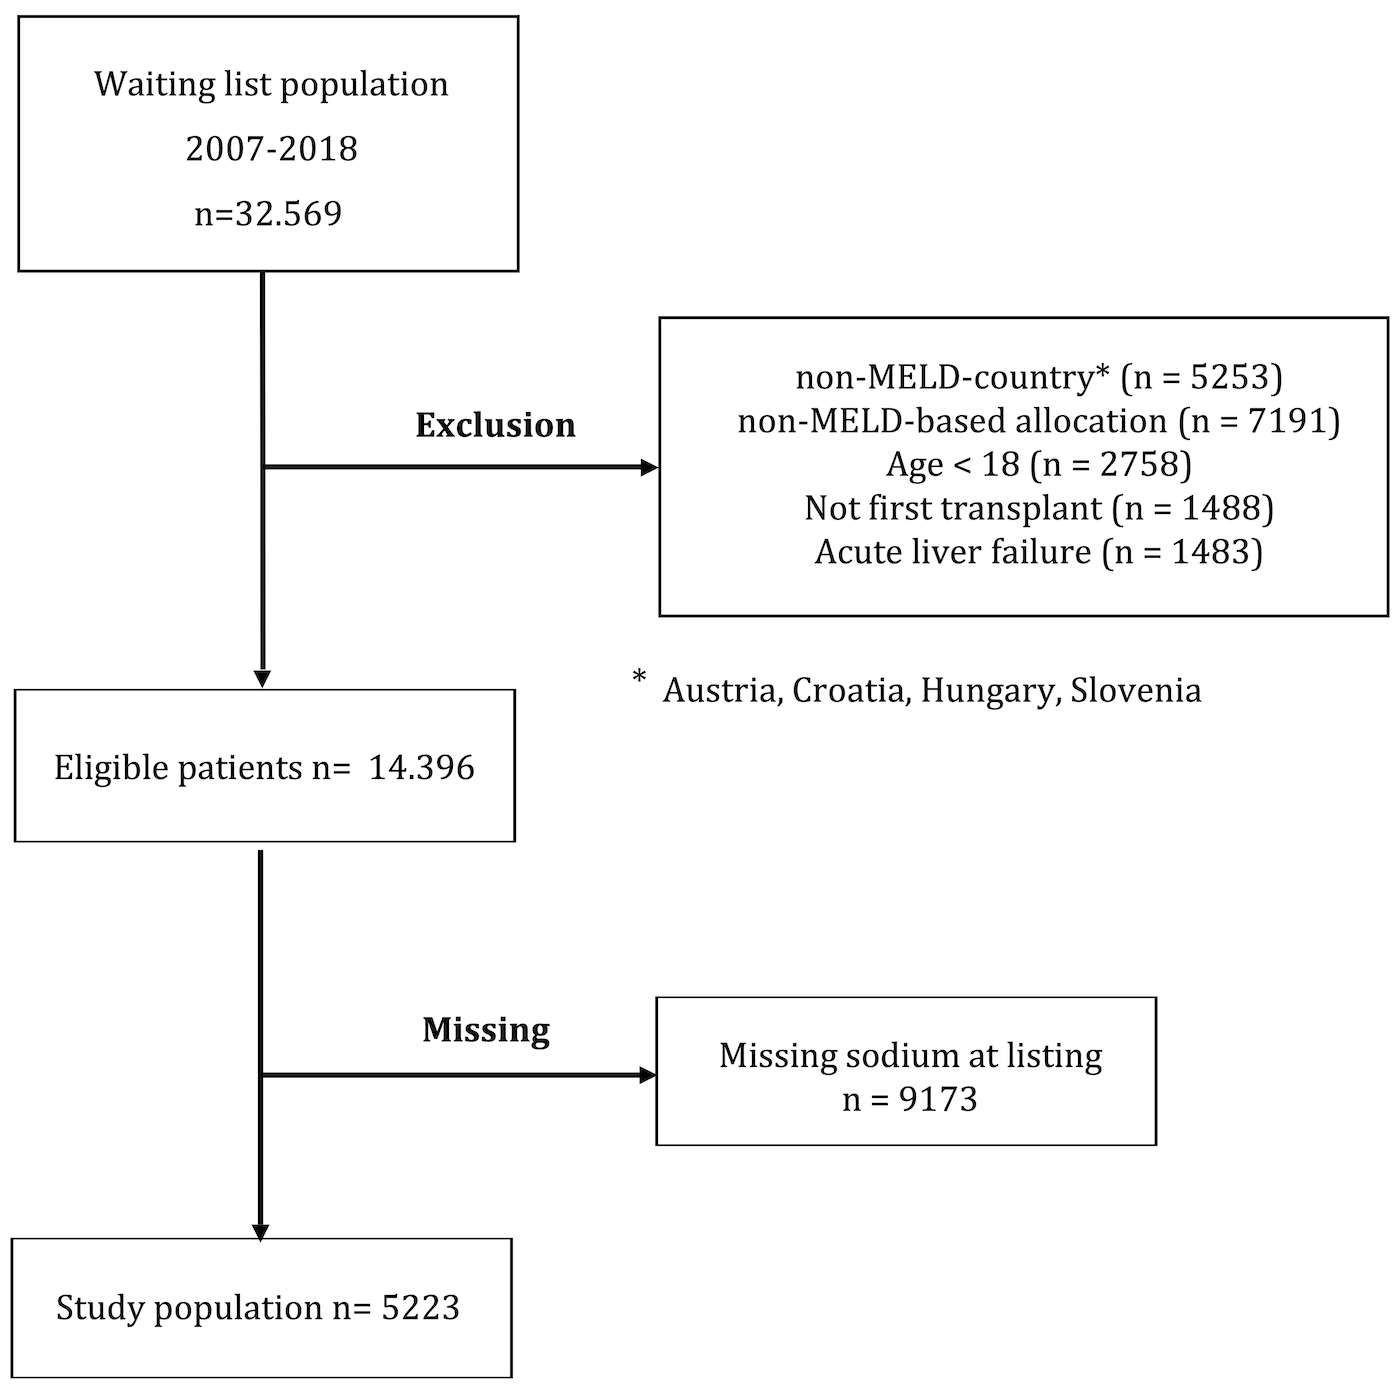
\includegraphics{figures/meldna/figure 1. in- exclusion.pdf}
\caption{\label{fig:meldna-fig1}The flowchart of in- and exclusion for this study}
\end{figure}

For this study, 14.396 patients were eligible. After excluding patients with missing serum Na at listing, 5223 patients were included. See Figure \ref{fig:meldna-fig1}. The baseline characteristics of included patients at first active listing are shown in Table \ref{tab:meldna-tab1}. The median lab MELD score was 16 (IQR 11-21) and the median sodium concentration was 137 (IQR 134-140) mmol/L. Hyponatremia of \textless135, \textless130, and \textless125 mmol/L was found in respectively 28.5\%, 8.8\%, and 2.6\% of the patients. Patients with alcohol-induced cirrhosis (ALD) had the lowest median Na levels, see Figure \ref{fig:meldna-fig2}.

\begin{figure}
\centering
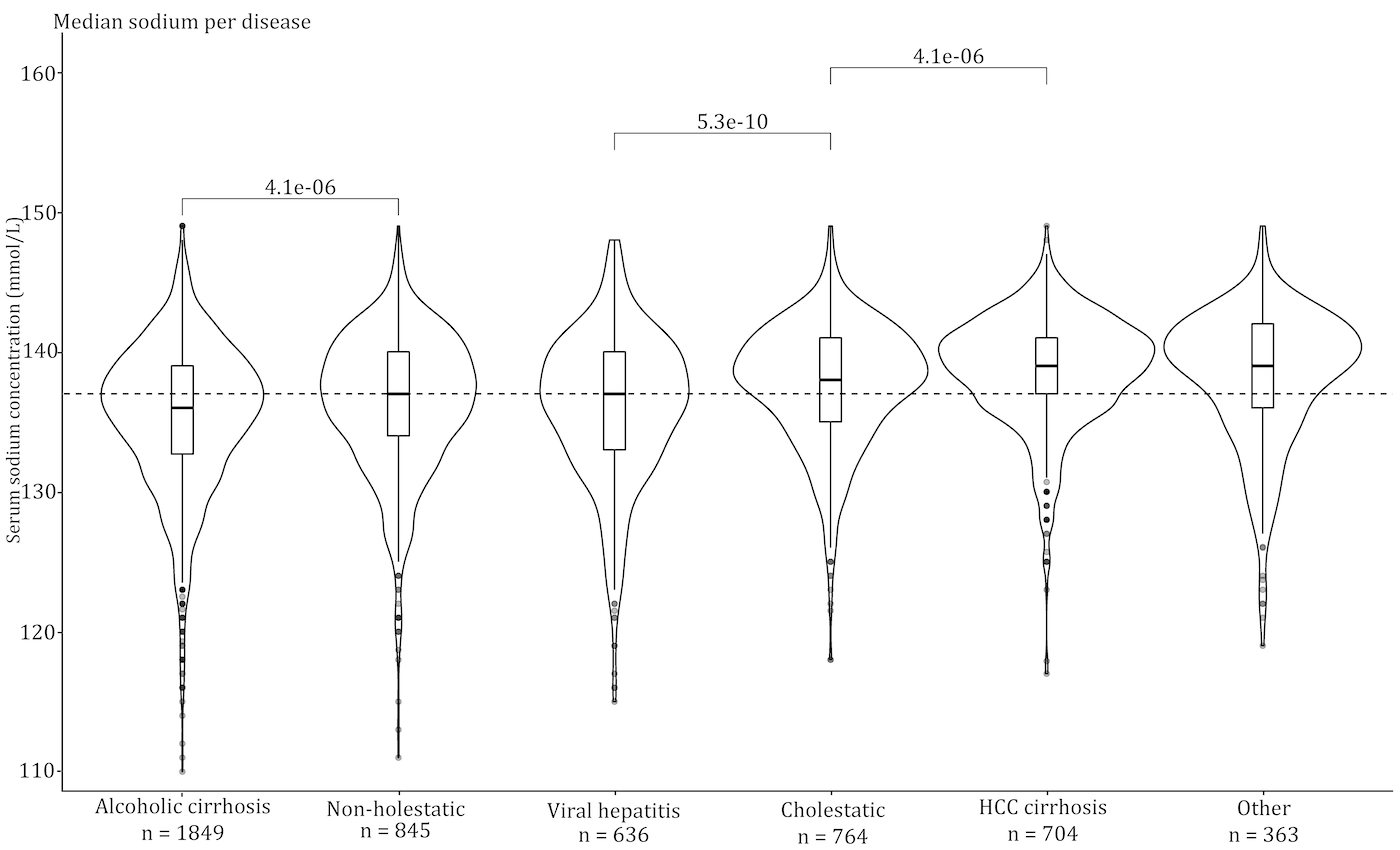
\includegraphics{figures/meldna/figure 2. median sodium per disease.pdf}
\caption{\label{fig:meldna-fig2}Violin plots with embedded box plots of the median serum sodium (Na) levels at listing, for the most frequent causes of liver disease. The dotted line represents the median Na of 137 mmol/L for the whole cohort. For the significant differences between Na levels, P values for pairwise comparisons are shown}
\end{figure}

For the assessment of selection bias, an analysis of all eligible patients (Na present versus absent) was added (supplement 1). Compared to the included patients, eligible patients with missing serum Na were more often female (31.9\% vs 35.5\%) and had higher rates of alcohol- or virus-induced liver cirrhosis (respectively 35.9\% vs 41.0\% and 12.4\% vs 15.3\%, p\textless0.001). MELD scores were comparable, but excluded patients had significantly higher creatinine levels at listing (1.36 vs 1.42 mg/dL p\textless0.001).

\begin{figure}
\centering
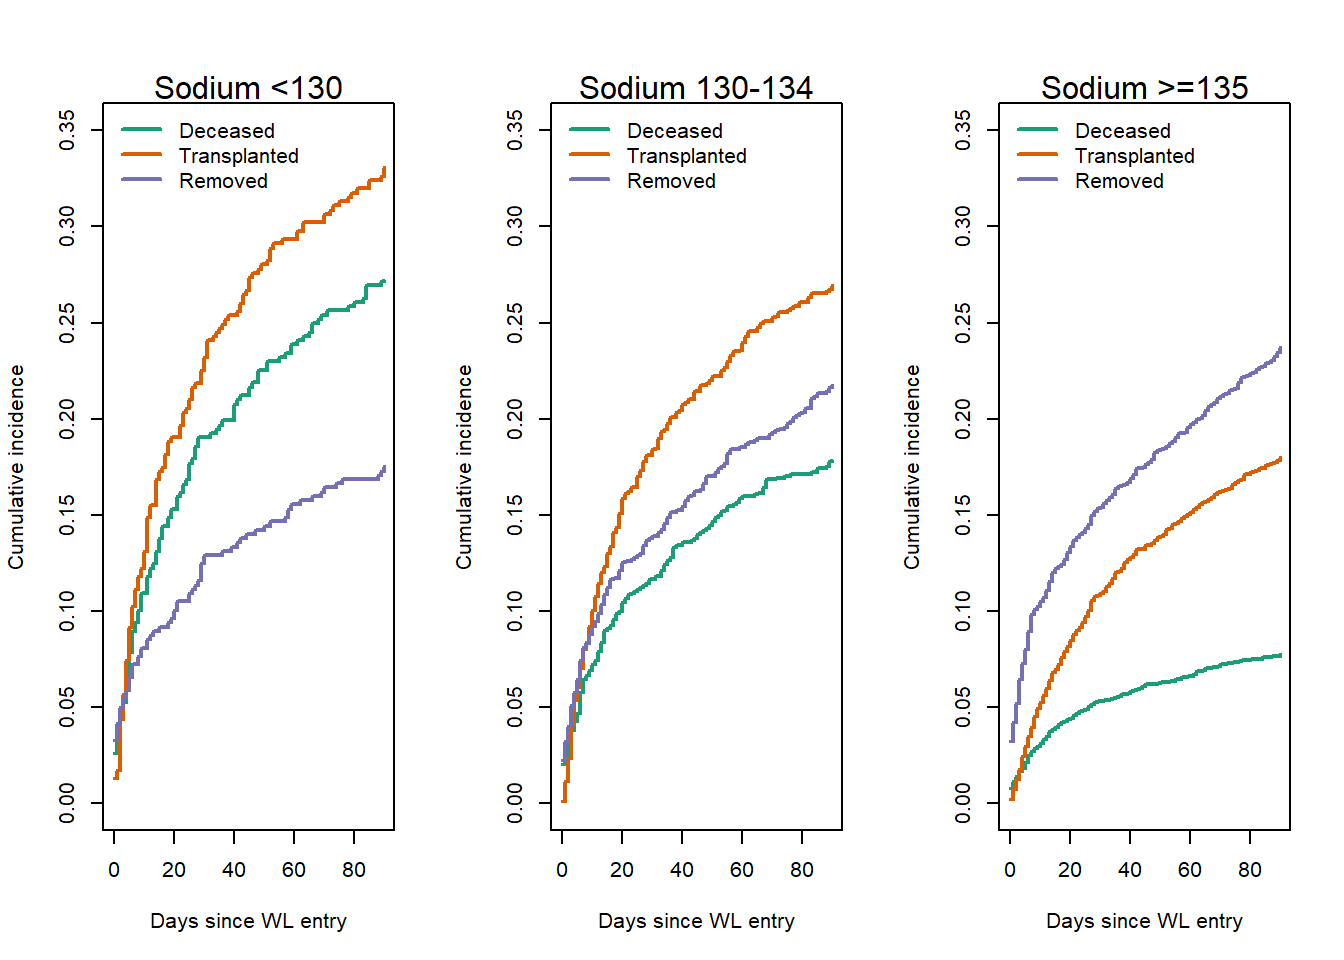
\includegraphics{thesis_files/figure-latex/meldna-fig3-1.pdf}
\caption{\label{fig:meldna-fig3}Cumulative incidence plots for 90-day WL outcomes, with competing risks of death, transplantation and removal due to clinical condition or censoring for NSE or HU status during waiting. Hyponatriemic patients show increased rates of mortality (27\%) and transplantation (33\%) compared to normonatriemic patients (respectively 8\% and 18\%).}
\end{figure}

Competing risk analysis showed that 90-day mortality and transplantation rates increased as sodium levels decreased, see Figure \ref{fig:meldna-fig3}. Na\textless130, 130-134 and \textgreater=135 patients had 90-day death risks of respectively 27\%, 18\% and 8\%. The 90-day transplant rates were respectively 33\%, 27\% and 18.0\%. The grouped Na levels showed diverging survival curves, i.e.~at lower Na levels the mortality risk increased at a higher rate (supplement 2). The 90-day death HRs for Na \textless130 and Na 130-134 compared to Na \textgreater=135 patients were 4.72 (95\%CI 3.81-5.83), and 2.72 (95\%CI 2.26-3.28), respectively.

\hypertarget{meld-na-performance}{%
\subsection*{MELD-Na performance}\label{meld-na-performance}}
\addcontentsline{toc}{subsection}{MELD-Na performance}

\begin{figure}
\centering
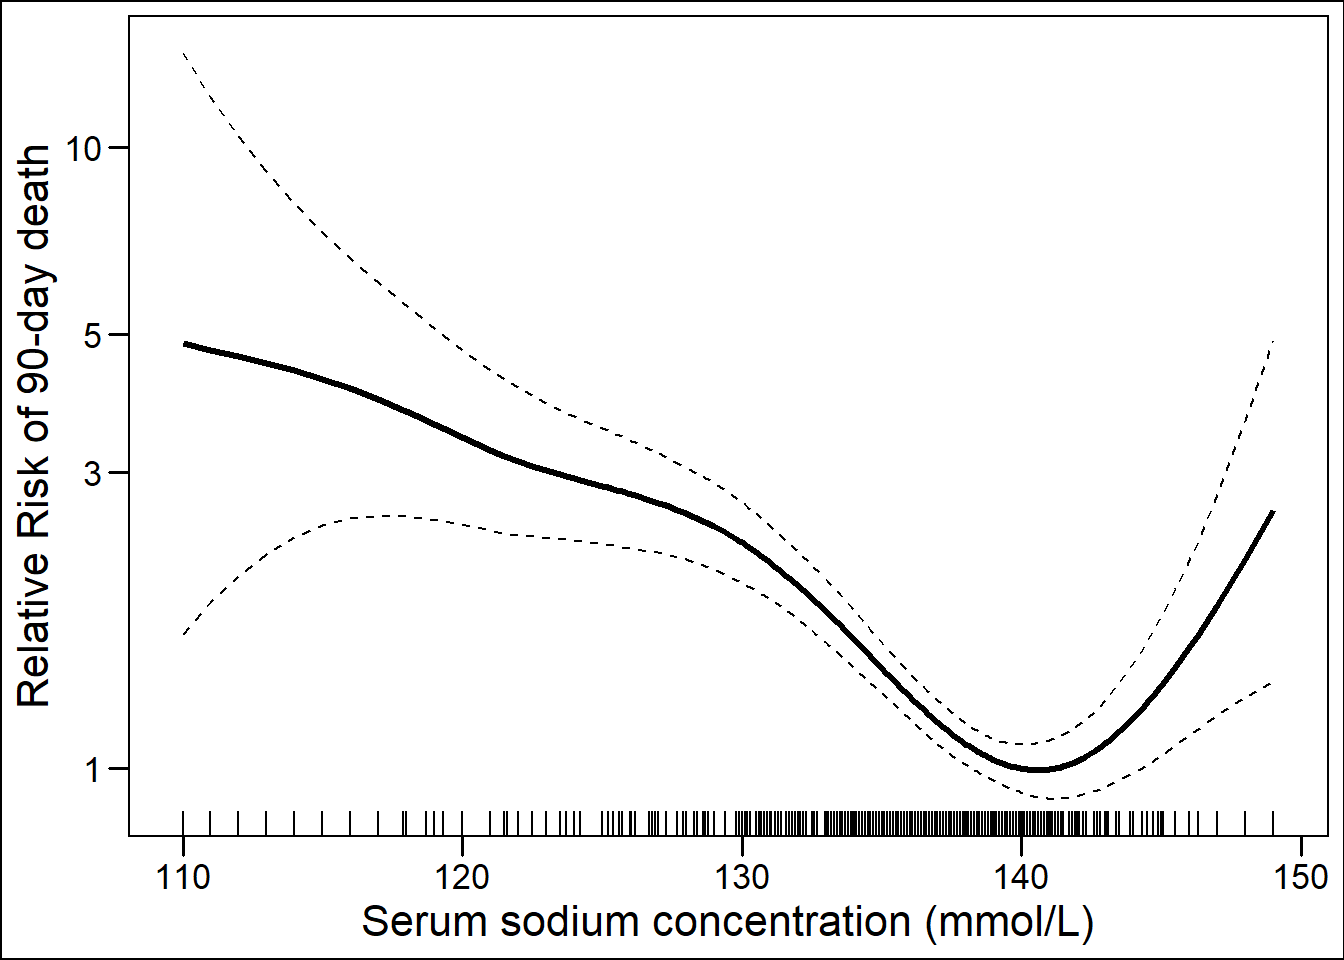
\includegraphics{thesis_files/figure-latex/meldna-fig4-1.pdf}
\caption{\label{fig:meldna-fig4}Generalized additive Cox model with spline showing the effect of serum sodium at listing on 90-day mortality, corrected for the MELD score.}
\end{figure}

Per MELD point increase, the 90-day mortality risk increased by 17\% (HR 1.17; 95\%CI 1.16 -- 1.18; p\textless0.001), c-index 0.832 (SE 0.008). The GAM with splines of the MELD-corrected effect of Na level on 90-day mortality showed approximate linearity in the 125-140 mmol/L range, see Figure \ref{fig:meldna-fig4}. Within this interval, the risk of 90-day death increased by threefold (HR 2.9; 95\%CI 2.30-3.53; p\textless0.001). In the MELD-Na model, each gained MELD and lowered Na point increased 90-day mortality risk by respectively 16\% (HR 1.16; 95\%CI 1.15 -- 1.17; p\textless0.001), and 8\% (HR 0.92; 95\%CI 0.90 -- 0.94; p\textless0.001), c-index 0.847 (SE 0.007).

\begin{figure}
\centering
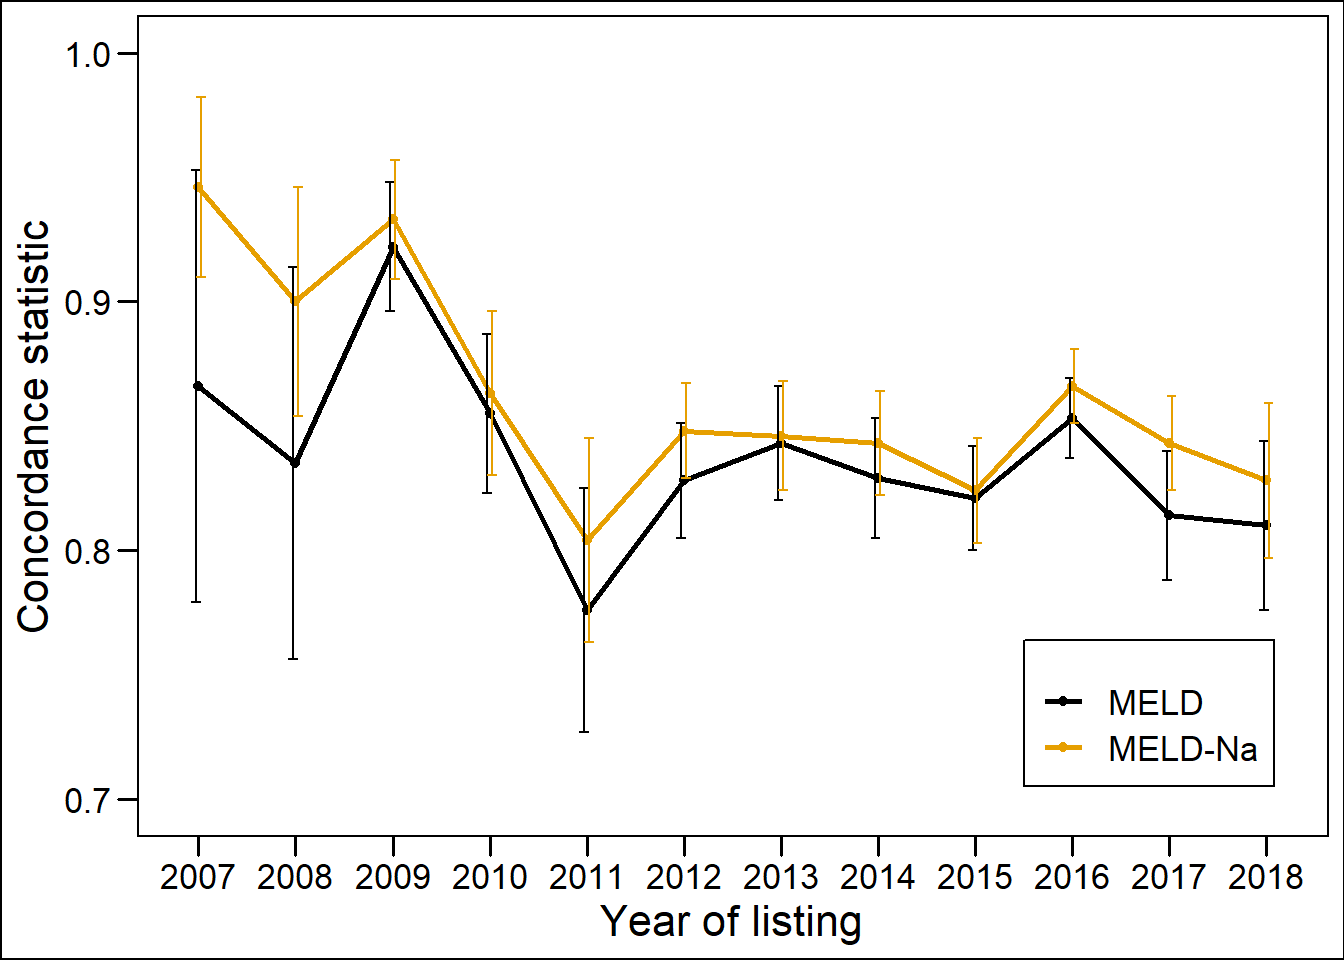
\includegraphics{thesis_files/figure-latex/meldna-fig5-1.pdf}
\caption{\label{fig:meldna-fig5}The concordance statistics (c-indices) for 90-day mortality of MELD and MELD-Na between 2007 and 2018.}
\end{figure}

For each year of the study period, the c-index of MELD and MELD-Na was plotted, see Figure \ref{fig:meldna-fig5}. Between 2007-2018, the c-index of MELD and MELD-Na decreased significantly, respectively from 0.866 to 0.810 and 0.946 to 0.828 (Table \ref{tab:meldna-tab2} ). In this period, the MELD, age and distribution of liver disease changed significantly (supplement 4). Alcohol-induced liver disease, HCC, primary biliary cirrhosis (PBC) and non-alcoholic steatohepatitis (NASH) cirrhosis increased and primary sclerosing cholangitis (PSC), hepatitis-C (HCV), hepatitis-B (HBV) and other causes decreased.

\linespread{1}

\begin{table}

\caption{\label{tab:meldna-tab2}The 90-day mortality concordance statistics of MELD and MELD-Na}
\centering
\begin{tabular}[t]{rrrrr}
\toprule
Year & MELD & SE & MELD-Na & SE\\
\midrule
\cellcolor{gray!6}{2007} & \cellcolor{gray!6}{0.866} & \cellcolor{gray!6}{0.087} & \cellcolor{gray!6}{0.946} & \cellcolor{gray!6}{0.036}\\
2008 & 0.835 & 0.079 & 0.900 & 0.046\\
\cellcolor{gray!6}{2009} & \cellcolor{gray!6}{0.922} & \cellcolor{gray!6}{0.026} & \cellcolor{gray!6}{0.933} & \cellcolor{gray!6}{0.024}\\
2010 & 0.855 & 0.032 & 0.863 & 0.033\\
\cellcolor{gray!6}{2011} & \cellcolor{gray!6}{0.776} & \cellcolor{gray!6}{0.049} & \cellcolor{gray!6}{0.804} & \cellcolor{gray!6}{0.041}\\
2012 & 0.828 & 0.023 & 0.848 & 0.019\\
\cellcolor{gray!6}{2013} & \cellcolor{gray!6}{0.843} & \cellcolor{gray!6}{0.023} & \cellcolor{gray!6}{0.846} & \cellcolor{gray!6}{0.022}\\
2014 & 0.829 & 0.024 & 0.843 & 0.021\\
\cellcolor{gray!6}{2015} & \cellcolor{gray!6}{0.821} & \cellcolor{gray!6}{0.021} & \cellcolor{gray!6}{0.824} & \cellcolor{gray!6}{0.021}\\
2016 & 0.853 & 0.016 & 0.866 & 0.015\\
\cellcolor{gray!6}{2017} & \cellcolor{gray!6}{0.814} & \cellcolor{gray!6}{0.026} & \cellcolor{gray!6}{0.843} & \cellcolor{gray!6}{0.019}\\
2018 & 0.810 & 0.034 & 0.828 & 0.031\\
\bottomrule
\end{tabular}
\end{table}

\linespread{1.213}

\begin{figure}
\centering
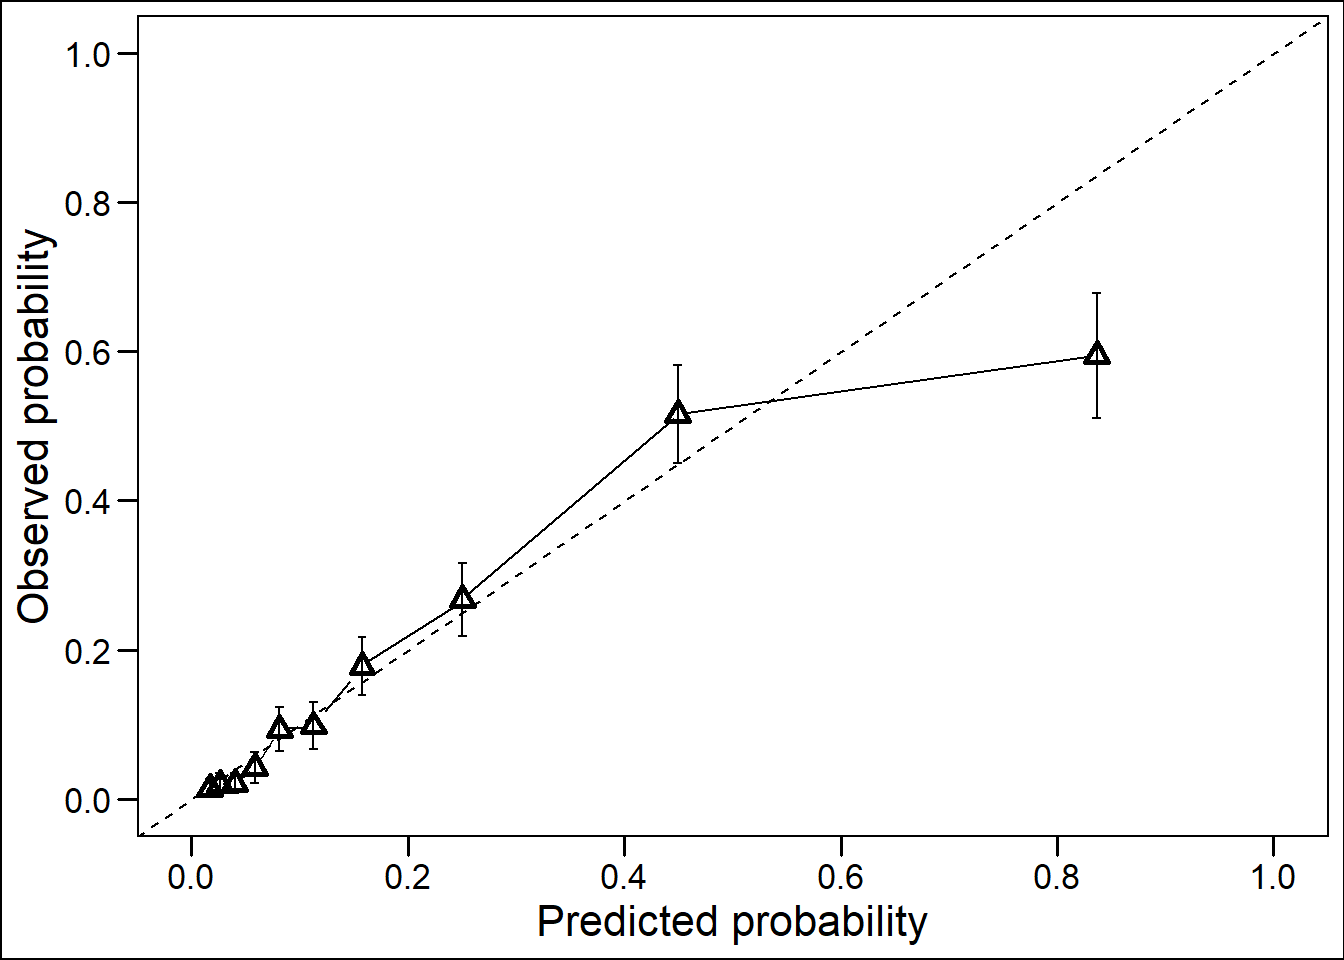
\includegraphics{thesis_files/figure-latex/meldna-fig6-1.pdf}
\caption{\label{fig:meldna-fig6}Calibration plot of the MELD-Na model showing the predicted and observed risks of death per decile (10\%) of the patient population. The diagonal line represents perfect calibration.}
\end{figure}

The MELD-Na calibration plot showed a well calibrated model for 90\% of the predicted risks in the population, with an overestimation for the highest 10\% (504 patients) predicted risks (Figure \ref{fig:meldna-fig6} and supplement 6). The prediction error of 90-day death was lower for MELD-Na than for MELD, with Brier scores of respectively 0.059 (34\% prediction error reduction), and 0.061 (32\% reduction).

\hypertarget{impact-on-the-waiting-list}{%
\subsection*{Impact on the waiting list}\label{impact-on-the-waiting-list}}
\addcontentsline{toc}{subsection}{Impact on the waiting list}

On the WL, implementation of the MELD-Na score would lead to competition for transplantation between hyponatremic and high-MELD patients. The constructed heatmap of risk differences showed that compared to MELD, approximately 20\% of the patients gained significant predicted 90-day mortality risks according to MELD-Na (red area). The largest increase (+22.5\%) was found for MELD 23 Na 125 patients. Approximately 19\% of the patients had significantly lower predicted risks with MELD-Na compared to MELD (blue area), of which the largest decrease (-8.72\%) was estimated for MELD 27 Na 140 patients, see Figure \ref{fig:meldna-fig7}.

\begin{figure}
\subfloat[Gained MELD-Na points for each combination of MELD and serum sodium level at listing\label{fig:meldna-fig7-1}]{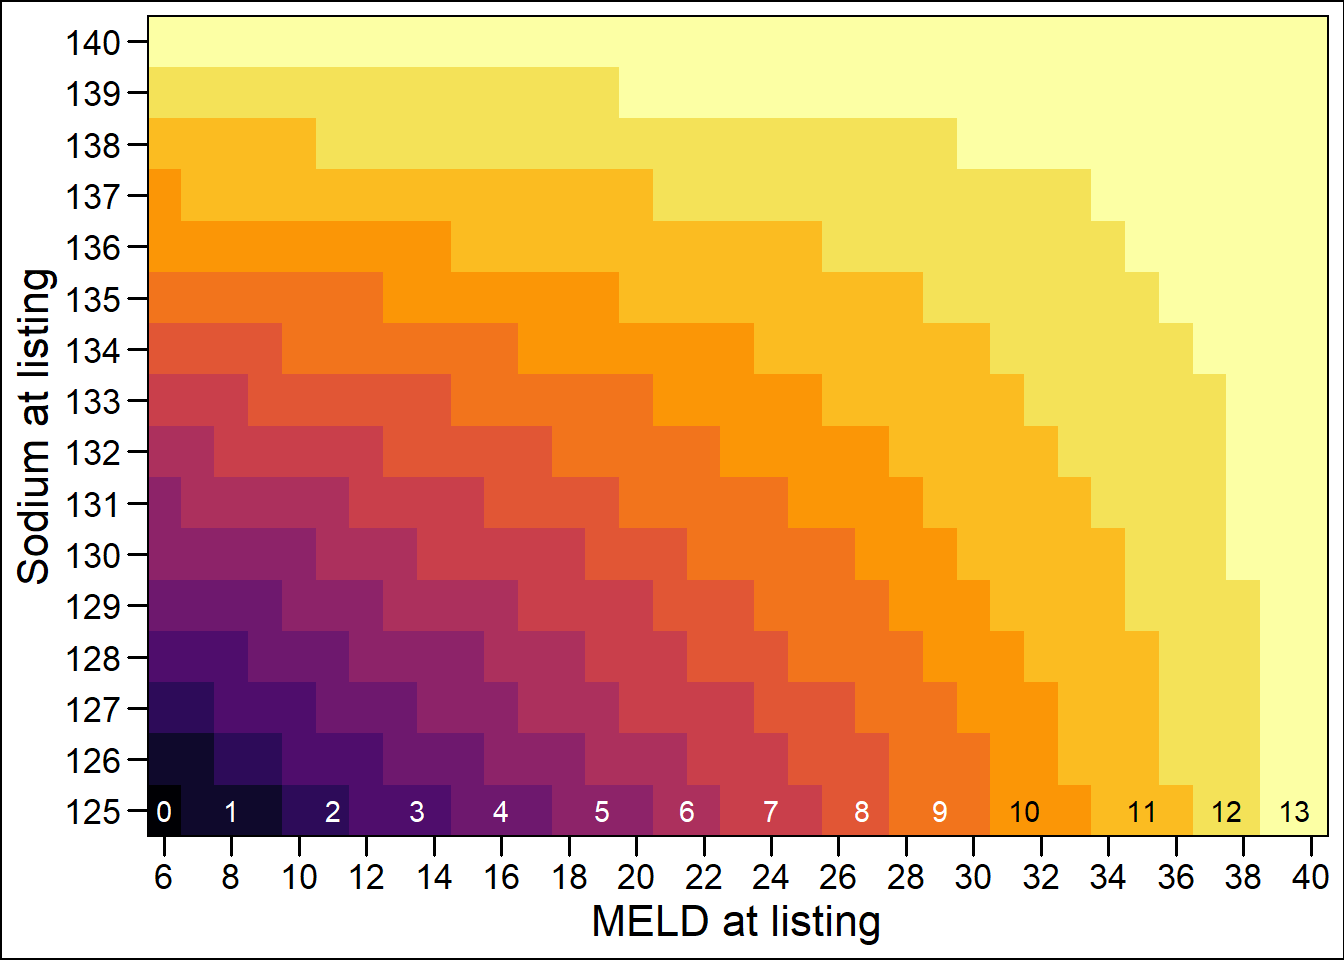
\includegraphics{thesis_files/figure-latex/meldna-fig7-1} }\newline\subfloat[Difference in predicted death probability between MELD and MELD-Na\label{fig:meldna-fig7-2}]{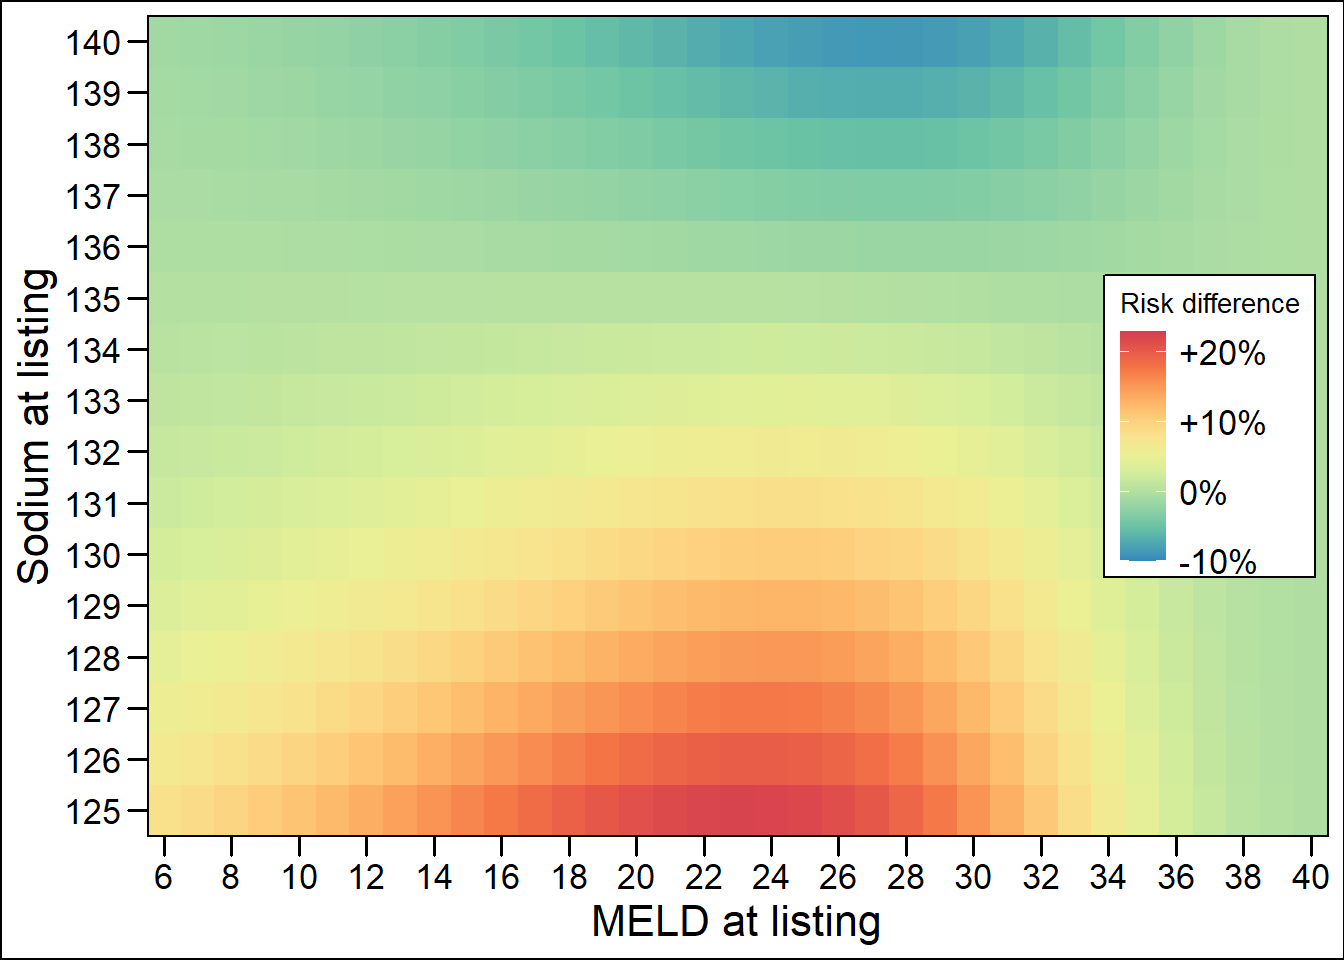
\includegraphics{thesis_files/figure-latex/meldna-fig7-2} }\caption{Point and risk differences between MELD and MELD-Na.}\label{fig:meldna-fig7}
\end{figure}

Thus, the patients in the red area (19\%) are prioritized most by MELD-Na. On the other hand, the lowest 20\% of predicted risks (blue area) would have a reduced chance of transplantation compared to MELD allocation. The interactive heatmaps allow specific assessment of the gained risks and MELD-Na points for individual patients (online supplement \url{https://plot.ly/~Liver_Research/3/} and \url{https://plot.ly/~Liver_Research/5/}). In total, 3384 (64.9\%) patients gained an average of 1.94 MELD-Na points at listing. The highest reclassification rates, i.e.~lowest percentage on the diagonal, were seen between MELD 12 to 30 (figure 8 and \url{https://plot.ly/~Liver_Research/7/} and \url{https://plot.ly/~Liver_Research/18/}). On average, MELD 23 patients gained the most, i.e.~an average of 2.73, MELD-Na points. From 19 points and above, the frequency of MELD-Na scores at listing was significantly higher than MELD scores, with the exception of MELD 40 (online supplement \url{https://plot.ly/~Liver_Research/11/}).

To make comparison to the UNOS data possible, we calculated the stratified MELD reclassification rates and estimated WL mortality reduction (supplement 3). Stratification of scores in accordance to Kim et al.\textsuperscript{9} showed a reclassification rate of 26.3\% (156 / 593) in the deceased patients. This led to an estimated 4.9\% reduction in 90-day waiting list mortality. The analysis of disease-specific prioritization in the deceased patients showed that patients with HCC and hepatitis B had the highest chance of reclassification to a higher MELD-Na stratum, 36\% and 30\% respectively (supplement 3). However, patients with (post)alcoholic cirrhosis had the highest increase in mean MELD-Na compared to MELD. This illustrated that the strata chosen by Kim et al.~could enable stage migration bias (supplement 3 and 5). Therefore, we believe that the total number of reclassified patients and the distribution of the gained MELD-Na points are more useful information when estimating the possible impact of MELD-Na-based allocation (Figure \ref{fig:meldna-fig8} and \url{https://plot.ly/~Liver_Research/7/} and \url{https://plot.ly/~Liver_Research/18/}).

\begin{figure}
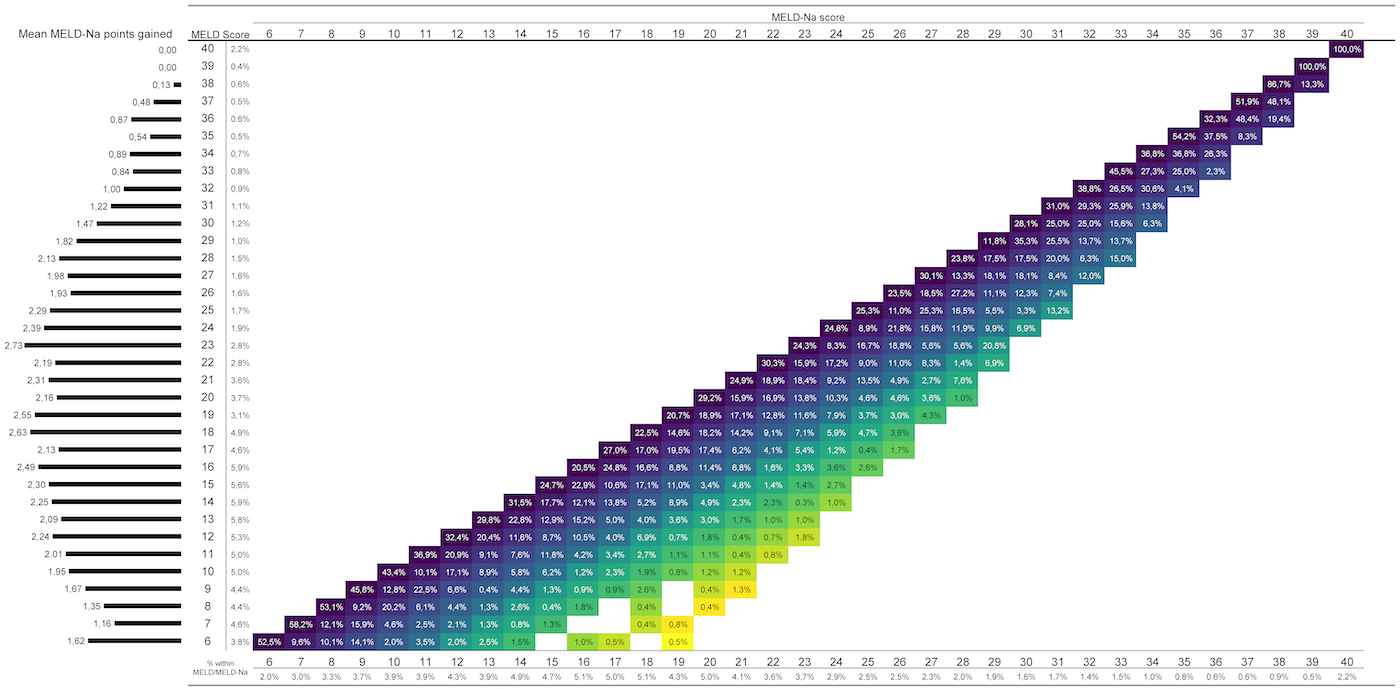
\includegraphics[angle=90]{figures/meldna/figure 8. Reclassification and gained points histogram 2} \caption{Reclassification from MELD (y-axis with percentage of patients with that score) to MELD-Na (x-axis with percentage of patients with that score). The diagonal shows which patients remain in the same stratum, that is, not reclassified, and which patients are reclassified to a higher MELD-Na score (percentages in the tiles). A lighter color indicates a higher difference between MELD and MELD-Na scores. The histogram on the left shows for each MELD score the average gain in MELD-Na points.}\label{fig:meldna-fig8}
\end{figure}

\hypertarget{discussion}{%
\section*{Discussion}\label{discussion}}
\addcontentsline{toc}{section}{Discussion}

This cohort analysis validated the UNOS MELD-Na score for the Eurotransplant region and provided the first examination of the extent of hyponatremia among LT candidates in this region. It was shown that the mortality hazards for mild and severely hyponatremic patients continued to increase during waiting for LT. The precise relation between the sodium concentration at listing and the 90-day WL mortality was calculated. Our analysis showed that MELD-Na had better prognostic abilities than MELD for the prediction of 90-day WL mortality, even though both MELD and MELD-Na declined the past years. Therefore, the use of the MELD-Na score could improve the allocation of donor livers in the Eurotransplant region.

\hypertarget{meld-na-prediction-performance}{%
\subsubsection*{MELD-Na prediction performance}\label{meld-na-prediction-performance}}
\addcontentsline{toc}{subsubsection}{MELD-Na prediction performance}

Accounting for serum sodium is relevant for the Eurotransplant population, as the prevalence of hyponatremia was similar,\textsuperscript{9,22} or even higher compared to another large study.\textsuperscript{28} The severity of hyponatremia was associated with a continuous increase in the risk of death on the WL, as shown by the cumulative incidence plots and diverging survival curves (Figure \ref{fig:meldna-fig3} and supplement 2). Compared to MELD, MELD-Na showed better discrimination between death and survival at 90-days, with a c-index of respectively 0.832 and 0.847. The c-index of MELD-Na was higher than found by some\textsuperscript{29} and comparable to that found by other investigators.\textsuperscript{9,30} Although the improvement in c-index by using MELD-Na was modest, it represented an important improvement in mortality prediction by considering hyponatremia as an independent risk factor of 90-day mortality. As the sickest candidates on the waiting list are prioritized, the increased discrimination would improve allocation.

Although MELD-Na performed better than MELD, both models showed significantly declining c-indices between 2007-2018 (Figure \ref{fig:meldna-fig5}, Table \ref{tab:meldna-tab2} ). It is possible that the exceptionally high MELD-Na c-indices in the years 2007-2009 were due to population sampling, which would also make the decrease in c-index over the years seem excessive. In this period, average age and MELD at listing increased significantly. Most importantly, the distribution of causes of liver disease significantly changed (supplement 4). Compared to the US, the Eurotransplant population comprised more patients with ALD and HCC and less with HCV and NASH.\textsuperscript{24} Godfrey et al.~first showed declining c-indices over the years for MELD and MELD-Na, which they attributed to the decrease in HCV and increase of NASH and ALD. Despite the different distribution of causes of liver disease compared to the US, a similar change over time was seen. This could explain the initially higher but similarly declining c-indices of MELD and MELD-Na. Policy makers should consider this decline when evaluating a possible shift from MELD to MELD-Na. Still, MELD-Na would be a significant improvement because of the increasing prevalence of hyponatremia, its effect on 90-day mortality and the significantly higher c-indices of MELD-Na.

The MELD-Na showed good calibration, with overestimation of risks only in the top 10\% of the patients. Both MELD and MELD-Na overestimated the highest predicted risks (supplement 6), as also shown by others.\textsuperscript{9} However, MELD-Na showed a higher reduction in the prediction error of 90-day death compared to MELD, as calculated with Brier scores. Thus, MELD-Na was a more accurate predictor of 90-day WL death than MELD alone.

\hypertarget{effect-of-meld-na}{%
\subsubsection*{Effect of MELD-Na}\label{effect-of-meld-na}}
\addcontentsline{toc}{subsubsection}{Effect of MELD-Na}

Since we validated the UNOS MELD-Na score, we used the Na 125-140 mmol/L interval to fit our model. In this interval we showed a 1.5 higher increase in 90-day mortality risk per Na unit as compared to the UNOS regions.\textsuperscript{9} Therefore, a greater reduction in WL mortality could be achieved through MELD-Na-based allocation. In the US, introduction of MELD-Na-based allocation reduced (HR 0.738) 90-day waiting list mortality for almost all MELD scores.\textsuperscript{22} However, the number of transplants was higher in the studied MELD-Na period, which also could have reduced WL mortality. Still, Nagai et al.~showed that the intended recognition of hyponatremia was achieved, as the WL mortality hazards of mild and severe hyponatremia decreased with respectively 27.9\% and 48.3\%.\textsuperscript{22} In the US, it was shown that in MELD\textless12 patients hyponatremia was not associated with LT survival benefit.\textsuperscript{20} Thus, UNOS MELD-Na is only used to allocate liver grafts in MELD\textgreater11 patients. In our population, very few (2.8\%) MELD\textless12 patients had severe hyponatremia. Although these patients would gain transplant chances through MELD-Na allocation, others would be prioritized more often. Our data also showed that the frequency of MELD-Na \textgreater18 scores increased significantly (\url{https://plot.ly/~Liver_Research/11/}). This would reduce transplant chances for patients listed with exception points, e.g.~HCC patients, as these patients initially receive 20 points at listing in Eurotransplant.\textsuperscript{6} Although the reduced advantage of (N)SE points is warranted according to some,\textsuperscript{31,32} (N)SE point policy did not change after MELD-Na implementation in the UNOS regions (personal SRTR communication). Still, many patients are listed with exception points, both in Eurotransplant and in the US. Therefore, the distribution of gained MELD-Na points, survival benefit and influence on exception points of Eurotransplant LT candidates should be considered before implementation of MELD-Na-based allocation. A simulation of MELD-Na-based allocation would give the most accurate estimates of the effect on WL mortality.

\hypertarget{limitations}{%
\subsubsection*{Limitations}\label{limitations}}
\addcontentsline{toc}{subsubsection}{Limitations}

This study has several limitations. First, only one measurement, i.e.~at first listing, of the MELD and sodium was used to study the effect on 90-day mortality. Since the disease state of the patient is a dynamic process, a time-dependent analysis with more datapoints might have been a better representation of the true risk posed by hyponatremia. Indeed, we showed that the effect of hyponatremia increased with time (Figure \ref{fig:meldna-fig3} and supplement 3). Also, serum sodium levels in the MELD-Na model were bound between 125-140 mmol/L. The fitted Cox model between these borders had a excellent c-index, but the relationship between serum sodium level and mortality was slightly different for the Eurotransplant region compared to the UNOS regions.\textsuperscript{9} However, the goal was to validate the MELD-Na as used in the UNOS regions for the Eurotransplant region, and this goal was achieved. Still, refitting of the MELD parameters for the Eurotransplant population could be valuable, especially regarding the decline in c-index between 2007-2018. Second, sodium data at first listing was missing for many eligible patients (supplement 1). This could have caused selection bias, possibly making the results less generalizable. However, analysis of the differences between the patients with and without registered sodium at listing showed that there was no reason to suspect selection bias. In the missing Na group, a significantly higher prevalence of alcoholic cirrhosis and virus-induced hepatitis was seen (supplement 4). Also, patients in the group with missing Na had a significantly higher serum creatinine. Thus, the prevalence of hyponatremia in those eligible patients could very well be even higher than found in the current cohort. Moreover, even though some data was missing, the number of patients included in this study sufficed to evaluate and estimate the improvements of MELD-Na with great statistical precision. Thus, the results of this study should be an incentive for the mandatory collection of sodium values across the Eurotransplant region.

\hypertarget{conclusion}{%
\section*{Conclusion}\label{conclusion}}
\addcontentsline{toc}{section}{Conclusion}

In conclusion, this study showed that the MELD-Na gave better 90-day mortality prediction than MELD for LT candidates on the Eurotransplant waiting list. As stated before, ``the MELD-based allocation system will and also must evolve.''\textsuperscript{26} The recognition of the independent prognostic impact of hyponatremia should lead to a more effective allocation. Thus, in the Eurotransplant region the MELD should be replaced by the MELD-Na as the basis allocation of donor livers.

\newpage
\linespread{1}
\small

\hypertarget{references-1}{%
\section*{References}\label{references-1}}
\addcontentsline{toc}{section}{References}

\begin{enumerate}
\def\labelenumi{\arabic{enumi}.}
\tightlist
\item
  Eurotransplant. Annual Report 2017.; 2018. www.eurotransplant.org.
\item
  Ng M, Fleming T, Robinson M, et al.~Global, regional, and national prevalence of overweight and obesity in children and adults during 1980-2013: A systematic analysis for the Global Burden of Disease Study 2013. Lancet. 2014;384(9945):766-781. \url{doi:10.1016/S0140-6736(14)60460-8}
\item
  Asrani SK, Devarbhavi H, Eaton J, Kamath PS. Burden of liver diseases in the world. J Hepatol. 2019;70(1):151-171. \url{doi:10.1016/j.jhep.2018.09.014}
\item
  Pimpin L, Cortez-Pinto H, Negro F, et al.~Burden of liver disease in Europe: Epidemiology and analysis of risk factors to identify prevention policies. J Hepatol. 2018;69(3):718-735.
\item
  Estes C, Razavi H, Loomba R, Younossi Z, Sanyal AJ. Modeling the epidemic of nonalcoholic fatty liver disease demonstrates an exponential increase in burden of disease. Hepatology. 2018;67(1):123-133. \url{doi:10.1002/hep.29466}
\item
  Jochmans I, Van Rosmalen M, Pirenne J, Samuel U. Adult Liver Allocation in Eurotransplant. Transplantation. 2017;101(7):1542-1550. \url{doi:10.1097/TP.0000000000001631}
\item
  Malinchoc M, Kamath PS, Gordon FD, Peine CJ, Rank J, Ter Borg PCJ. A model to predict poor survival in patients undergoing transjugular intrahepatic portosystemic shunts. Hepatology. 2000;31(4):864-871. \url{doi:10.1053/he.2000.5852}
\item
  Biggins SW, Rodriguez HJ, Bacchetti P, Bass NM, Roberts JP, Terrault NA. Serum sodium predicts mortality in patients listed for liver transplantation. Hepatology. 2005;41(1):32-39. \url{doi:10.1002/hep.20517}
\item
  Kim WR, Biggins SW, Kremers WK, et al.~Hyponatremia and Mortality among Patients on the Liver-Transplant Waiting List. N Engl J Med. 2008;359(10):1018-1026. \url{doi:10.1007/s11250-017-1262-3}
\item
  Ruf AE, Kremers WK, Chavez LL, Descalzi VI, Podesta LG, Villamil FG. Addition of serum sodium into the MELD score predicts waiting list mortality better than MELD alone. Liver Transplant. 2005;11(3):336-343. \url{doi:10.1002/lt.20329}
\item
  Heuman DM, Abou-Assi SG, Habib A, et al.~Persistent ascites and low serum sodium identify patients with cirrhosis and low MELD scores who are at high risk for early death. Hepatology. 2004;40(4):802-810. \url{doi:10.1002/hep.1840400409}
\item
  Biggins SW, Kim WR, Terrault NA, et al.~Evidence-Based Incorporation of Serum Sodium Concentration Into MELD. Gastroenterology. 2006;130(6):1652-1660. \url{doi:10.1053/j.gastro.2006.02.010}
\item
  Ginès P, Guevara M. Hyponatremia in cirrhosis: Pathogenesis, clinical significance, and management. Hepatology. 2008;48(3):1002-1010. \url{doi:10.1002/hep.22418}
\item
  John S, Thuluvath PJ. Hyponatremia in cirrhosis: Pathophysiology and management. World J Gastroenterol. 2015;21(11):3197-3205. \url{doi:10.3748/wjg.v21.i11.3197}
\item
  Wong F, Blei AT, Blendis LM, Thuluvath PJ. A vasopressin receptor antagonist (VPA-985) improves serum sodium concentration in patients with hyponatremia: A multicenter, randomized, placebo-controlled trial. Hepatology. 2003;37(1):182-191. \url{doi:10.1053/jhep.2003.50021}
\item
  Wong F, Sniderman K, Liu P, Allidina Y, Sherman M, Blendis L. Transjugular intrahepatic portosystemic stent shunt: Effects on hemodynamics and sodium homeostasis in cirrhosis and refractory ascites. Ann Intern Med. 1995;122(11):816-822. \url{doi:10.7326/0003-4819-122-11-199506010-00002}
\item
  Londoño MC, Guevara M, Rimola A, et al.~Hyponatremia Impairs Early Posttransplantation Outcome in Patients With Cirrhosis Undergoing Liver Transplantation. Gastroenterology. 2006;130(4):1135-1143. \url{doi:10.1053/j.gastro.2006.02.017}
\item
  Dawwas MF, Lewsey JD, Neuberger JM, Gimson AE. The Impact of Serum Sodium Concentration on Mortality After Liver Transplantation: A Cohort Multicenter Study. Liver Transplant. 2007;13(5):767-768. \url{doi:10.1002/lt}
\item
  Leise MD, Yun BC, Larson JJ, et al.~Effect of the Pretransplant Serum Sodium Concentration on Outcomes Following Liver Transplantation. Liver Transplant. 2014;14(20):687-697. \url{doi:10.1002/lt}
\item
  Sharma P, Schaubel DE, Goodrich NP, Merion RM. Serum Sodium and Survival Benefit of Liver Transplantation. Liver Transplant. 2015;21:308-313. \url{doi:10.1002/lt}.
\item
  Allocation of livers and liver- intestines. Organ Procurement and Transplantation Network Liver and Intestine Committee.
\item
  Nagai S, Chau LC, Schilke RE, et al.~Effects of Allocating Livers for Transplantation Based on Model for End-Stage Liver Disease-Sodium Scores on Patient Outcomes. Gastroenterology. 2018;155(October):1451-1482. \url{doi:10.1053/j.gastro.2018.07.025}
\item
  2017 Annual Data Report. Scientific Registry of Transplant Recipients. \url{http://srtr.transplant.hrsa.gov/annual_reports/Default.aspx}. Published 2017. Accessed September 5, 2019.
\item
  Godfrey EL, Malik TH, Lai JC, et al.~The decreasing predictive power of MELD in an era of changing etiology of liver disease. Am J Transplant. 2019;19(12):3299-3307. \url{doi:10.1111/ajt.15559}
\item
  Moons KGM, Altman DG, Reitsma JB, et al.~Transparent reporting of a multivariable prediction model for individual prognosis or diagnosis (TRIPOD): Explanation and elaboration. Ann Intern Med. 2015;162(1):W1-W73. \url{doi:10.7326/M14-0698}
\item
  Wiesner R, Edwards E, Freeman R, et al.~Model for end-stage liver disease (MELD) and allocation of donor livers. Gastroenterology. 2003;124(1):91-96. \url{doi:10.1053/gast.2003.50016}
\item
  Sievert C, Parmer C, Hocking T, et al.~Create Interactive Web Graphics via ``plotly.js.'' 2019. \url{https://plot.ly/r}.
\item
  Angeli P, Wong F, Watson H, et al.~Hyponatremia in cirrhosis: Results of a patient population survey. Hepatology. 2006;44(6):1535-1542. \url{doi:10.1002/hep.21412}
\item
  Biselli M, Gitto S, Gramenzi A, et al.~Six Score Systems to Evaluate Candidates with Advanced Cirrhosis for Orthotopic Liver Transplant: Which Is the Winner? Liver Transplant. 2010;16:964-973. \url{doi:10.1002/lt}.
\item
  Cejas N, Villamil F, Lendoire J, et al.~Improved Waiting-List Outcomes in Argentina After the Adoption of a Model for End-Stage Liver Disease--Based Liver Allocation Policy. Liver Transplant. 2013;13(19):711-720. \url{doi:10.1002/lt}
\item
  Northup PG, Intagliata NM, Shah NL, Pelletier SJ, Berg CL, Argo CK. Excess mortality on the liver transplant waiting list: Unintended policy consequences and model for End-Stage Liver Disease (MELD) inflation. Hepatology. 2015;61(1):285-291. \url{doi:10.1002/hep.27283}
\item
  Umgelter A, Hapfelmeier A, Kopp W, van Rosmalen M, Rogiers X, Guba M. Disparities in Eurotransplant liver transplantation wait-list outcome between patients with and without model for end-stage liver disease exceptions. Liver Transplant. 2017;23(10):1256-1265. \url{doi:10.1002/lt.24805}
\end{enumerate}

\newpage
\linespread{1.213}
\normalsize
\thispagestyle{plain}

\mbox{}

\pagecolor{black}
\color{white}

\hypertarget{chap-refit}{%
\chapter{Refitting the Model for End-stage Liver Disease for the Eurotransplant region}\label{chap-refit}}

\chaptermark{Refit MELD}

\vspace*{\fill}

\noindent Goudsmit BFJ, Putter H, Tushuizen ME, et al.~Refitting the Model for End-Stage Liver Disease for the Eurotransplant Region. \emph{Hepatology}. 2021;74(1):351-363. doi: 10.1002/hep.31677.

\begin{center}\rule{0.5\linewidth}{0.5pt}\end{center}

\newpage

\noindent
\nopagecolor
\color{black}
\small

\textbf{Abstract}

\textbf{Background \& Aims}: The United Network for Organ Sharing's Model for End- Stage Liver Disease (UNOS-MELD) score is the basis of liver allocation in the Eurotransplant region. It was constructed 20 years ago in a small US cohort and has remained unchanged ever since. The best boundaries and coefficients were never calculated for any region outside the United States. Therefore, this study refits the MELD (reMELD) for the Eurotransplant region.

\textbf{Methods}: All adult patients listed for a first LT between 01.01.2007-31.12.2018 were included. Data was randomly split in a training (70\%) and validation (30\%) set. In the training data, generalized additive models (GAMs) with splines were plotted for each MELD parameter. The lower and upper bound combinations with the maximum log-likelihood were chosen for the final models. The refit models were tested in the validation data with c-indices and Brier scores. Through likelihood ratio tests the refit models were compared to UNOS-MELD. The correlation between scores and survival of prioritized patients was calculated.

\textbf{Results}: A total of 6,684 patients were included. Based on training data, refit parameters were capped at creatinine 0.7-2.5 (mg/dL), bilirubin 0.3-27 (mg/dL), INR 0.1-2.6 and sodium 120-139 (mmol/L). ReMELD and reMELD-Na showed c-indices of 0.866 and 0.869 respectively. ReMELD-Na prioritized patients with 1.6 times higher 90-day mortality probabilities as compared to UNOS-MELD.

\textbf{Conclusion}: Refitting MELD resulted in new lower and upper bounds for each parameter. The predictive power of reMELD-Na was significantly higher than UNOS-MELD. Refit MELD prioritized patients with higher 90-day mortality rates. Thus, reMELD(-Na) should replace UNOS-MELD for liver graft allocation in the ET region.

\newpage
\normalsize

\hypertarget{introduction-1}{%
\section*{Introduction}\label{introduction-1}}
\addcontentsline{toc}{section}{Introduction}

The number of patients in need of a liver transplantation (LT) in the Eurotransplant region exceeds the available donor grafts.\textsuperscript{1} Therefore, patients with end-stage liver disease are placed on a waiting list (WL) which prioritizes the patients with the most severe liver disease, i.e.~most in need of transplantation. The Model of End-stage Liver Disease (MELD) estimates disease severity in LT candidates, based on three parameters: serum creatinine, bilirubin and the international normalized ratio (INR) for prothrombin time.\textsuperscript{2} Since 2016, the UNOS regions also added serum sodium through the MELD-Na score,\textsuperscript{3} but the Eurotransplant region remains MELD-based. The MELD was weighed, i.e.~the relative importance of each parameter, based on a cohort from 1991-1995.\textsuperscript{4} For clinical use, the lower boundaries for the parameters were set to one, to prevent negative MELD scores after natural logarithm (\(ln\)) transformation. Creatinine levels were capped at four mg/dL for patients not receiving dialysis. According to some of the proposers of MELD, these boundaries were ``based entirely on the clinical intuition of the policy-making body when the MELD score was implemented.''\textsuperscript{5} Others also noted that ``arbitrary changes not based on mortality risk evidence were incorporated into the form of MELD'' and that these lower and upper limits were ``set without any particular objective rationale.''\textsuperscript{6}

On another continent and almost 20 years later, the original UNOS-MELD equation is still being used for the allocation of liver grafts in the Eurotransplant region and elsewhere. Due to changing population characteristics, the predictive power of UNOS MELD has declined significantly in the last years.\textsuperscript{7} However, an update of the MELD coefficients in UNOS data showed that performance could still be further improved.\textsuperscript{5} As the Eurotransplant population differs from the original MELD cohort,\textsuperscript{4,8} improvement of the Eurotransplant liver allocation is very well possible by refitting MELD to the Eurotransplant population. Refitting is the reweighing of predictors and establishment of lower and upper bounds of each parameter, based on the best fit to the current data. It was hypothesized that the UNOS-MELD is not optimally fit for the Eurotransplant patients, as it was fit on the UNOS population. This could diminish MELDs predictive power and discrimination ability between survival and death. It is the optimization of this discrimination that gives the most effective sickest-first allocation.

Therefore, this study constructs a refit MELD score for the Eurotransplant region, by reweighing the MELD coefficients and re-evaluating the boundaries for the three parameters based on recent Eurotransplant data. The refitting methods presented here could be used to improve prediction models for any region. Also, the added value of the serum sodium (Na) levels at listing in an Eurotransplant refit MELD-Na score will be evaluated. The performance of the constructed refit Eurotransplant models will be compared to the UNOS-MELD.

\hypertarget{methods-1}{%
\section*{Methods}\label{methods-1}}
\addcontentsline{toc}{section}{Methods}

\hypertarget{patient-data}{%
\subsection*{Patient data}\label{patient-data}}
\addcontentsline{toc}{subsection}{Patient data}

The TRIPOD statement was used to report the development of the multivariate prediction models in this study.\textsuperscript{9} Data was requested from the Eurotransplant Database. All adult patients actively listed for a first liver transplantation between January 1\textsuperscript{st}, 2007 - December 31\textsuperscript{st}, 2018 were included. The starting point of inclusion was chosen after the start of MELD-based allocation in 2006. Patients were excluded if they received (non)standard exception points (NSE), a high urgency (HU) status (i.e.~UNOS status 1), living donor grafts or multi-organ transplantations (other than kidney).\textsuperscript{10} Patient data was collected from the date of active listing until delisting or the end of 90-day follow-up. Reasons for delisting were death, transplantation, removal because of clinical condition or other reasons. The primary outcome was death within 90 days of first active listing. The predictors used for the multivariate models were both the bound and continuous levels of serum creatinine, bilirubin, INR and sodium at first active listing. For the survival analysis, patients were censored at transplantation, removal from the list, end of follow-up at 31.12.2018 or after receiving NSE points or a HU status during active waiting. The sample size for this study was set by the retrospective design. Missing data (in \textless0.01\%) was not imputed.

\hypertarget{statistical-methods}{%
\subsection*{Statistical methods}\label{statistical-methods}}
\addcontentsline{toc}{subsection}{Statistical methods}

The data was randomly split into a training (70\%) and validation (30\%) set. For each recipient, the UNOS-MELD and MELD-Na score at first active listing were calculated.\textsuperscript{11,12} Then, the ET refit MELD (reMELD) score was constructed in the training data. For each MELD parameter, a multivariate generalized additive Cox model (GAM) with smoothing splines was plotted. The GAM showed the (non-)linear effect of the specific parameter on 90-day mortality, corrected for the other uncapped MELD parameters. By visual inspection it was assessed whether upper and lower boundaries for the parameter were necessary, i.e.~if there was any violation of the linearity relation between studied parameter and the 90-day mortality and at which point. Then, the best boundaries for the parameter were sought within the visually apparent range by calculating the maximum log-likelihood and the concordance statistic (c-index) for each possible combination of upper and lower bounds. The combination with the maximum log-likelihood was chosen as the lower and upper bound for that MELD parameter. The impact of deviations from the maximum log-likelihood and c-index were visualized through heatmaps to facilitate discussion of weighing the maximum calculated values against clinically relevant cut-offs. After establishing the best boundaries for the parameter, a multivariate Cox model with the capped parameter was compared to a Cox model with the unbounded values through likelihood ratio tests. To visualize the fit of the studied reMELD parameter, the obtained bounds and coefficient were plotted in the training data. The abovementioned steps were repeated for all three MELD parameters.

The three obtained capped parameters were then combined into a multivariate Cox model, thus forming the Eurotransplant refit MELD. To ensure equal distributions of the traditional UNOS-MELD and ET refit MELD scores in our data, the 25th and 75th quantiles were matched. Also, reMELD scores below 6 and above 40 were set to that value.
Then, the addition of serum sodium to the reMELD was investigated in the training set as described above for the MELD parameters. In short: based on the GAM inspection, the optimal Na bounds were sought, i.e.~calculating log-likelihood values and c-indices, and compared with likelihood ratio tests to uncapped Na levels. Interactions between Na and each refit MELD parameter were assessed and deemed relevant if p\textless0.01. Thus, the final reMELD-Na model comprised of reMELD parameters, newly bound sodium and relevant interactions between the terms. Again, the 25th and 75th quantiles were matched and the final scores of the refit MELD-Na were set between 6 to 40. Finally, the refit ET models were compared with likelihood ratio tests to UNOS-MELD. For each model, the c-index was calculated to calculate discriminative ability in the validation data. Brier scores were calculated as a measure of error reduction in prediction estimates.\textsuperscript{13} The fit of the models to the validation data was visualized by plotting the coefficients for each MELD parameter. The correlation between the currently used UNOS-MELD and constructed reMELD-Na was investigated by plotting both scores. To assess whether reMELD-Na would give more effective sickest-first allocation, survival estimates were calculated for patients prioritized by UNOS-MELD and reMELD-Na. All statistical analyses were performed using R v3.6.1(R Foundation for Statistical Computing, Vienna, Austria).

\hypertarget{results-1}{%
\section*{Results}\label{results-1}}
\addcontentsline{toc}{section}{Results}

\begin{table}

\caption{\label{tab:refit-tab1}Characteristics of training and validation data}
\centering
\resizebox{\linewidth}{!}{
\begin{threeparttable}
\begin{tabular}[t]{llll}
\toprule
characteristics & Training set & Validation set & p\\
\midrule
\cellcolor{gray!6}{n} & \cellcolor{gray!6}{4860} & \cellcolor{gray!6}{2084} & \cellcolor{gray!6}{}\\
Age (median (IQR)) & 56 (49-62) & 55 (49-62) & 0.022\\
\cellcolor{gray!6}{Gender female (\%)} & \cellcolor{gray!6}{1563 ( 32.2)} & \cellcolor{gray!6}{659 ( 31.6)} & \cellcolor{gray!6}{0.680}\\
\addlinespace[0.3em]
\multicolumn{4}{l}{\textbf{Disease (\%)}}\\
\hspace{1em}Cirrhosis, Alcoholic & 1361 ( 28.0) & 600 ( 28.8) & \\
\hspace{1em}\cellcolor{gray!6}{Cirrhosis, HCV} & \cellcolor{gray!6}{352 (  7.2)} & \cellcolor{gray!6}{123 (  5.9)} & \cellcolor{gray!6}{}\\
\hspace{1em}Cirrhosis, other causes & 825 (17.0) & 353 (16.9) & \\
\hspace{1em}\cellcolor{gray!6}{Cholestatic disease} & \cellcolor{gray!6}{652 (13.4)} & \cellcolor{gray!6}{295 (14.1)} & \cellcolor{gray!6}{}\\
\hspace{1em}HCC and cirrhosis & 953 ( 19.6) & 421 ( 20.2) & \\
\hspace{1em}\cellcolor{gray!6}{Other} & \cellcolor{gray!6}{717 (14.8)} & \cellcolor{gray!6}{292 (14.0)} & \cellcolor{gray!6}{}\\
\addlinespace[0.3em]
\multicolumn{4}{l}{\textbf{Status after 90 days}}\\
\hspace{1em}Censored because of HU or NSE & 1171 ( 24.2) & 476 ( 22.9) & \\
\hspace{1em}\cellcolor{gray!6}{Deceased} & \cellcolor{gray!6}{452 (9.30)} & \cellcolor{gray!6}{226 (  10.8)} & \cellcolor{gray!6}{}\\
\hspace{1em}Removed from the waiting list & 624 ( 12.8) & 257 ( 12.3) & \\
\hspace{1em}\cellcolor{gray!6}{Still waiting on waiting list} & \cellcolor{gray!6}{1734 ( 35.8)} & \cellcolor{gray!6}{739 ( 35.5)} & \cellcolor{gray!6}{}\\
\hspace{1em}Transplanted & 867 ( 17.9) & 381 ( 18.3) & \\
\cellcolor{gray!6}{Days follow-up (mean (SD))} & \cellcolor{gray!6}{44.22 (39.48)} & \cellcolor{gray!6}{44.06 (39.27)} & \cellcolor{gray!6}{0.875}\\
\addlinespace[0.3em]
\multicolumn{4}{l}{\textbf{Serum measurement at listing (mean (SD))}}\\
\hspace{1em}Creatinine in mg/dL & 1.40 (3.73) & 1.46 (4.16) & 0.563\\
\hspace{1em}\cellcolor{gray!6}{Bilirubin in mg/dL} & \cellcolor{gray!6}{5.74 (8.79)} & \cellcolor{gray!6}{5.84 (9.34)} & \cellcolor{gray!6}{0.669}\\
\hspace{1em}INR & 1.51 (0.72) & 1.52 (0.72) & 0.510\\
\hspace{1em}\cellcolor{gray!6}{Sodium in mmol/L} & \cellcolor{gray!6}{137.02 (4.99)} & \cellcolor{gray!6}{136.94 (4.88)} & \cellcolor{gray!6}{0.526}\\
UNOS MELD at listing (median (IQR)) & 14 (10-20) & 14 (10-20) & \\
\bottomrule
\end{tabular}
\begin{tablenotes}
\item \textit{Note: } 
\item IQR: inter quartile range, HCV: hepatitis C induced cirrhosis, HCC: hepatocellular carcinoma, HU: high urgency, NSE: (non)standard exception, SD: standard deviation, INR: international normalized ratio, UNOS: united network for organ sharing
\end{tablenotes}
\end{threeparttable}}
\end{table}

In this study, 6,944 patients were included, see Table \ref{tab:refit-tab1}. More male (68\%) than female patients were included, and alcohol induced cirrhosis was the most frequent cause of liver disease. The median UNOS-MELD and serum sodium at listing were 14 (IQR 10-20) and 138 (IQR 134-140) respectively. After 90 days of follow-up, 35.7\% of the patients were still waiting for LT, 23.8\% were censored due to HU status or (N)SE points, 18.0\% were transplanted, 12.6\% were removed from the WL and 9.8\% died on the WL. There were no relevant differences between the training and validation data.

\hypertarget{model-development}{%
\subsection*{Model development}\label{model-development}}
\addcontentsline{toc}{subsection}{Model development}

The GAM plots for each parameter are shown below. For creatinine, the S-shaped curve displayed clear lower and upper boundaries in Figure \ref{fig:refit-fig1}A, the maximum log-likelihood was calculated for the bounds of 0.7 and 2.5 mg/dL. Clinically, it seemed logical to include values of creatinine below 1.0 mg/dL, mainly because many patients (55\%) had creatinine levels \textless=1 mg/dL. Through refitting, the serum creatinine was decreased in weight and its upper bound was lowered. Therefore, the influence of renal failure on the chances for LT was reduced.

\begin{figure}

{\centering \subfloat[Creatinine\label{fig:refit-fig1-1}]{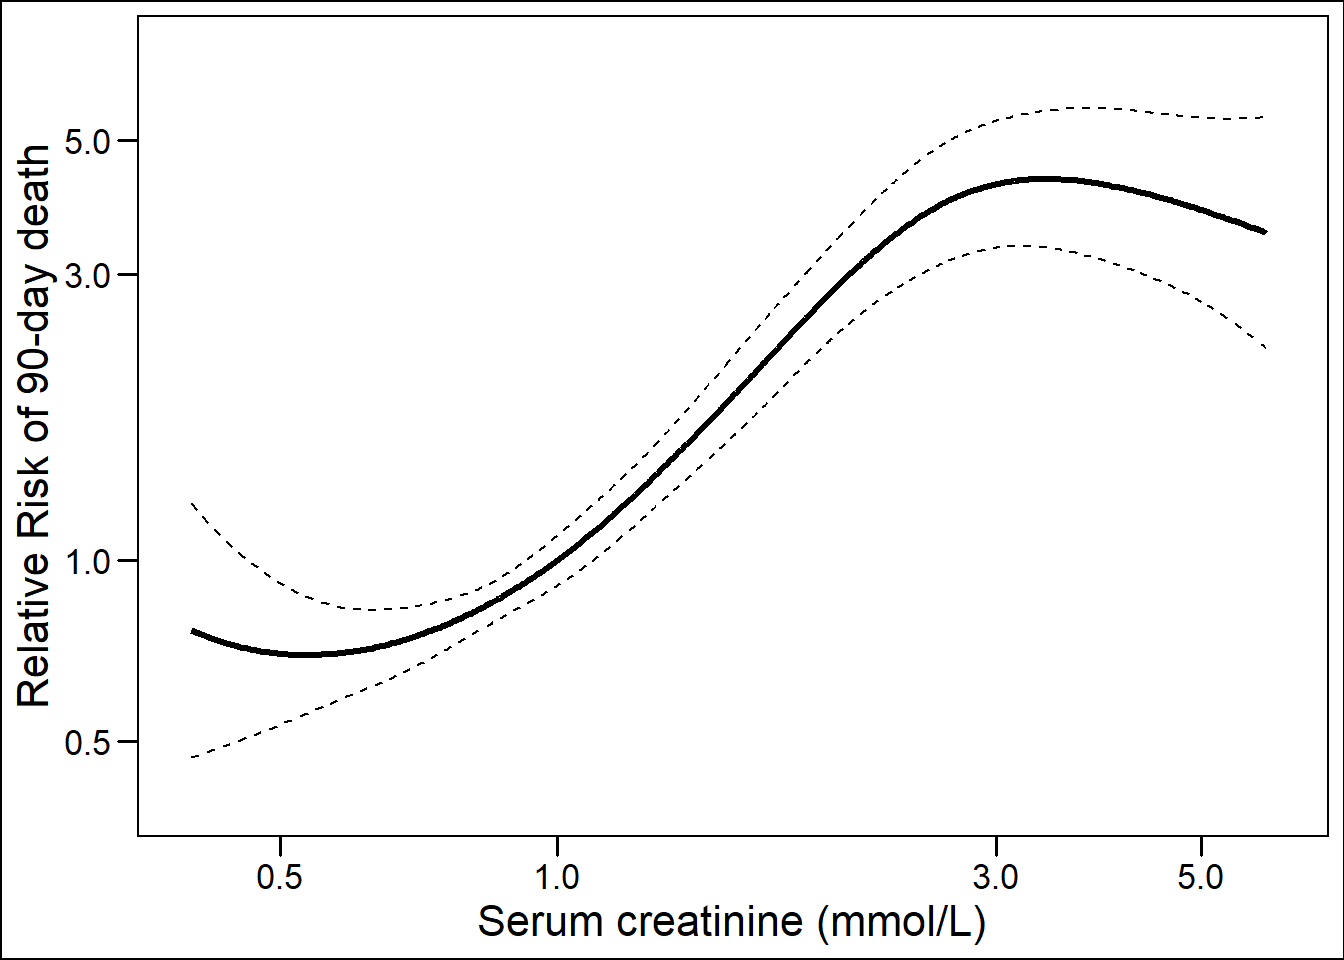
\includegraphics[height=0.27\textheight]{thesis_files/figure-latex/refit-fig1-1} }\newline\subfloat[Bilirubin\label{fig:refit-fig1-2}]{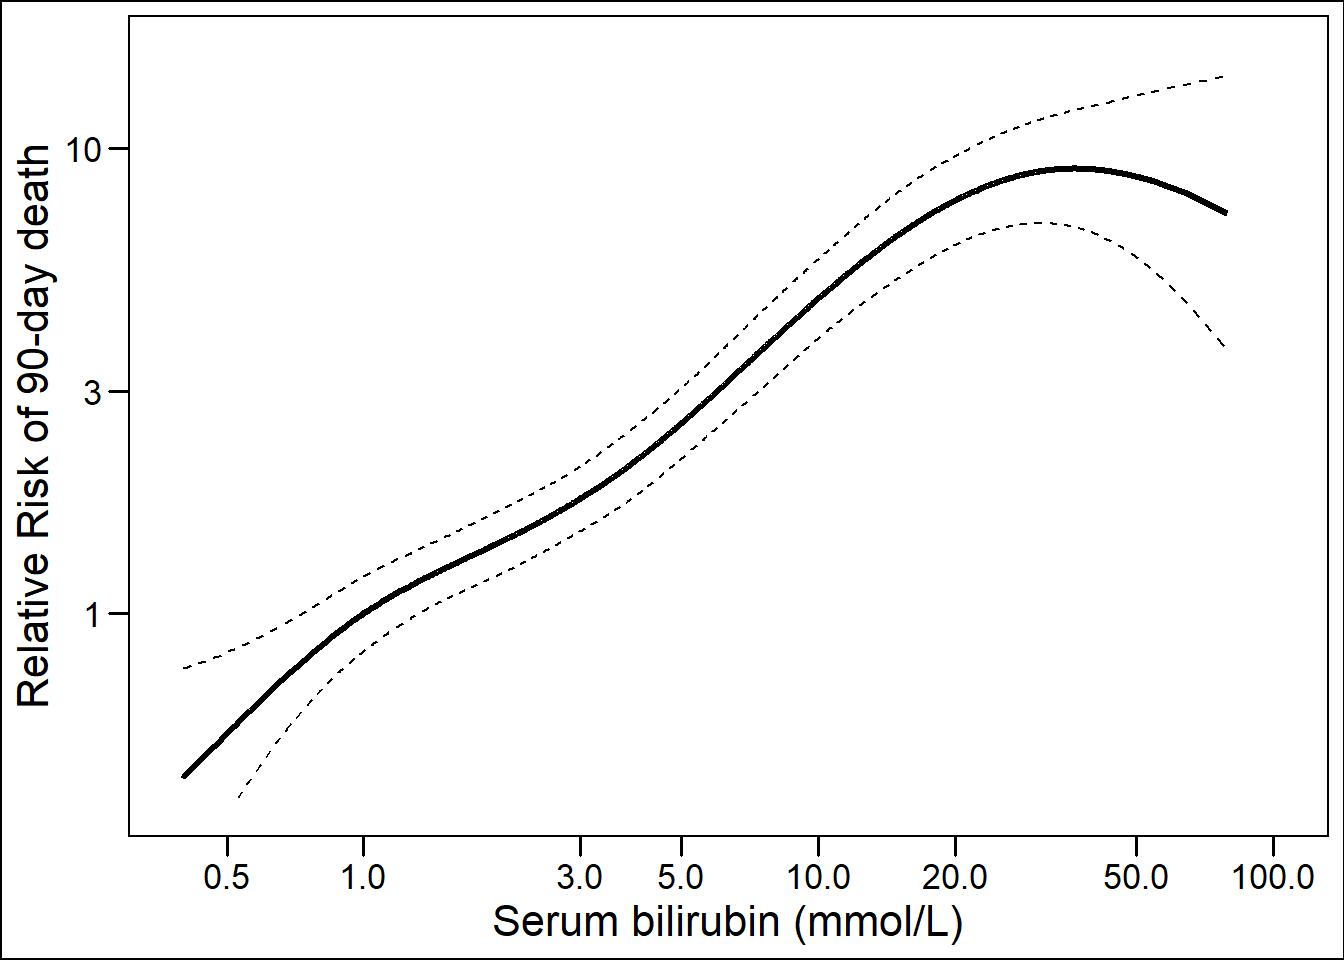
\includegraphics[height=0.27\textheight]{thesis_files/figure-latex/refit-fig1-2} }\newline\subfloat[INR\label{fig:refit-fig1-3}]{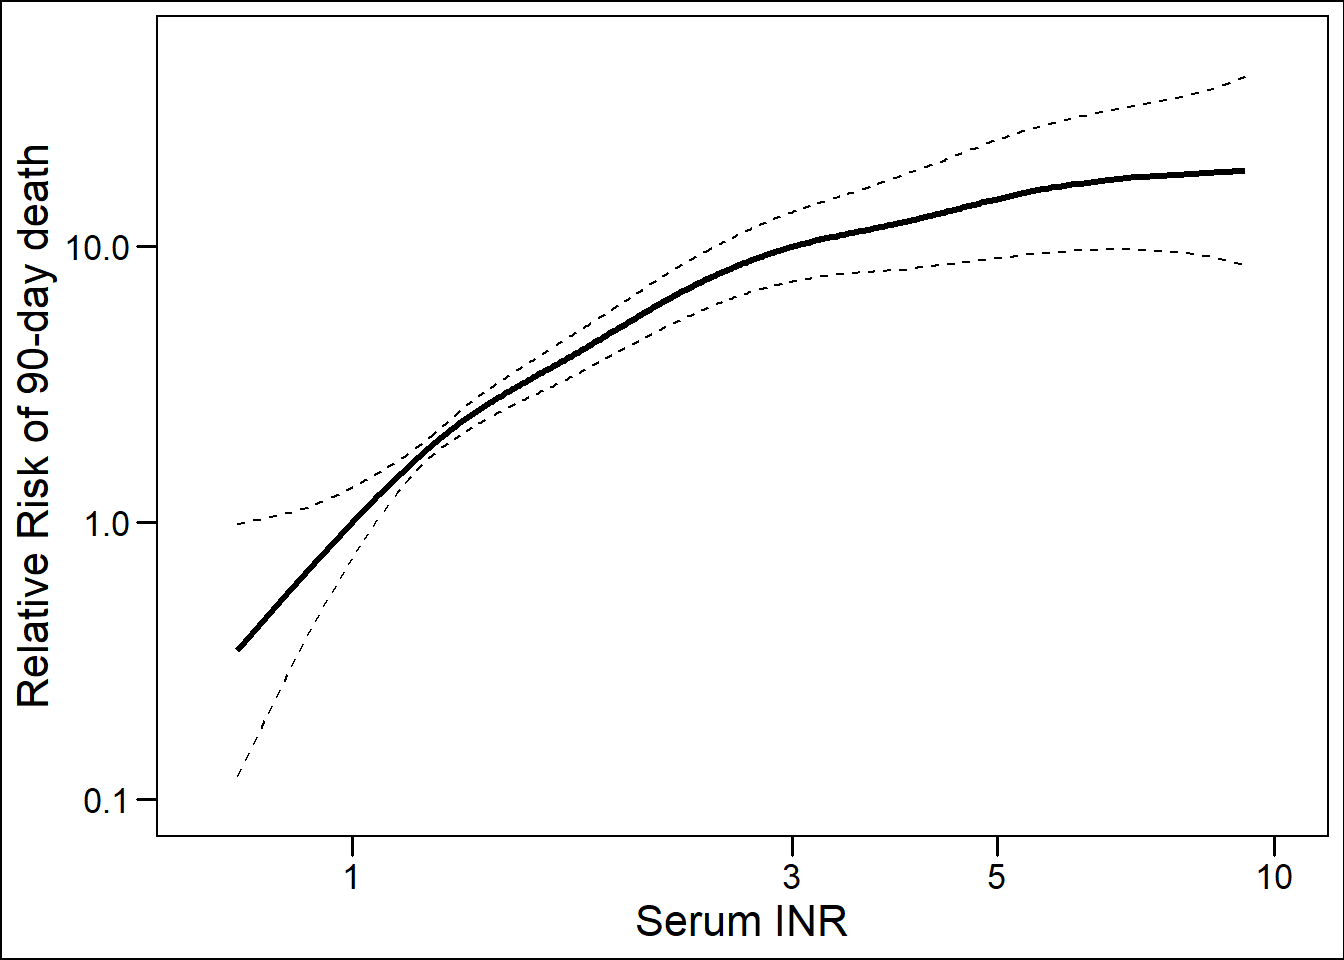
\includegraphics[height=0.27\textheight]{thesis_files/figure-latex/refit-fig1-3} }

}

\caption{For each parameter, the relation to 90-day mortality is shown based on the training data}\label{fig:refit-fig1}
\end{figure}

For bilirubin, in Figure \ref{fig:refit-fig1}B, the lower bound was found at 0.3 and the upper at 27 mg/dL. Varying of the lower bound between 0.1 and 0.5 did not alter the log-likelihood significantly, i.e.~would still be an acceptable fit to the data. Also, 23.7\% of our population would no longer be capped at listing. The upper bound of 27 mg/dL could be altered to a clinically more relevant value, roughly between 20 and 40, without affecting the optimal fit to the data too much (supplement heatmap bilirubin).

The INR had no lower bound and was capped at a maximum of 2.6, see Figure \ref{fig:refit-fig1}C. However, assessment of the log-likelihoods values showed that a range between 0.1 and 1.0 would be acceptable as lower bound (supplement heatmap INR) and would affect few patients (2.7\%). For the INR an upper bound of 2.6 was chosen, which still acknowledged, i.e.~did not cap, 93\% of the patients. Although it may seem controversial to cap the INR, this meant that if patients reached 2.6, they would receive the maximum refit points for INR, of which the weight was increased in the refit models.

Overall, the reMELD and reMELD-Na models capped less patients at assumed values than UNOS-MELD.
In Figure \ref{fig:refit-fig2}, lines were plotted for respectively creatinine, bilirubin, and the INR to represent the refit coefficient (slope of the diagonal) and the boundaries (horizontal lines).

\begin{figure}

{\centering \subfloat[Creatinine\label{fig:refit-fig2-1}]{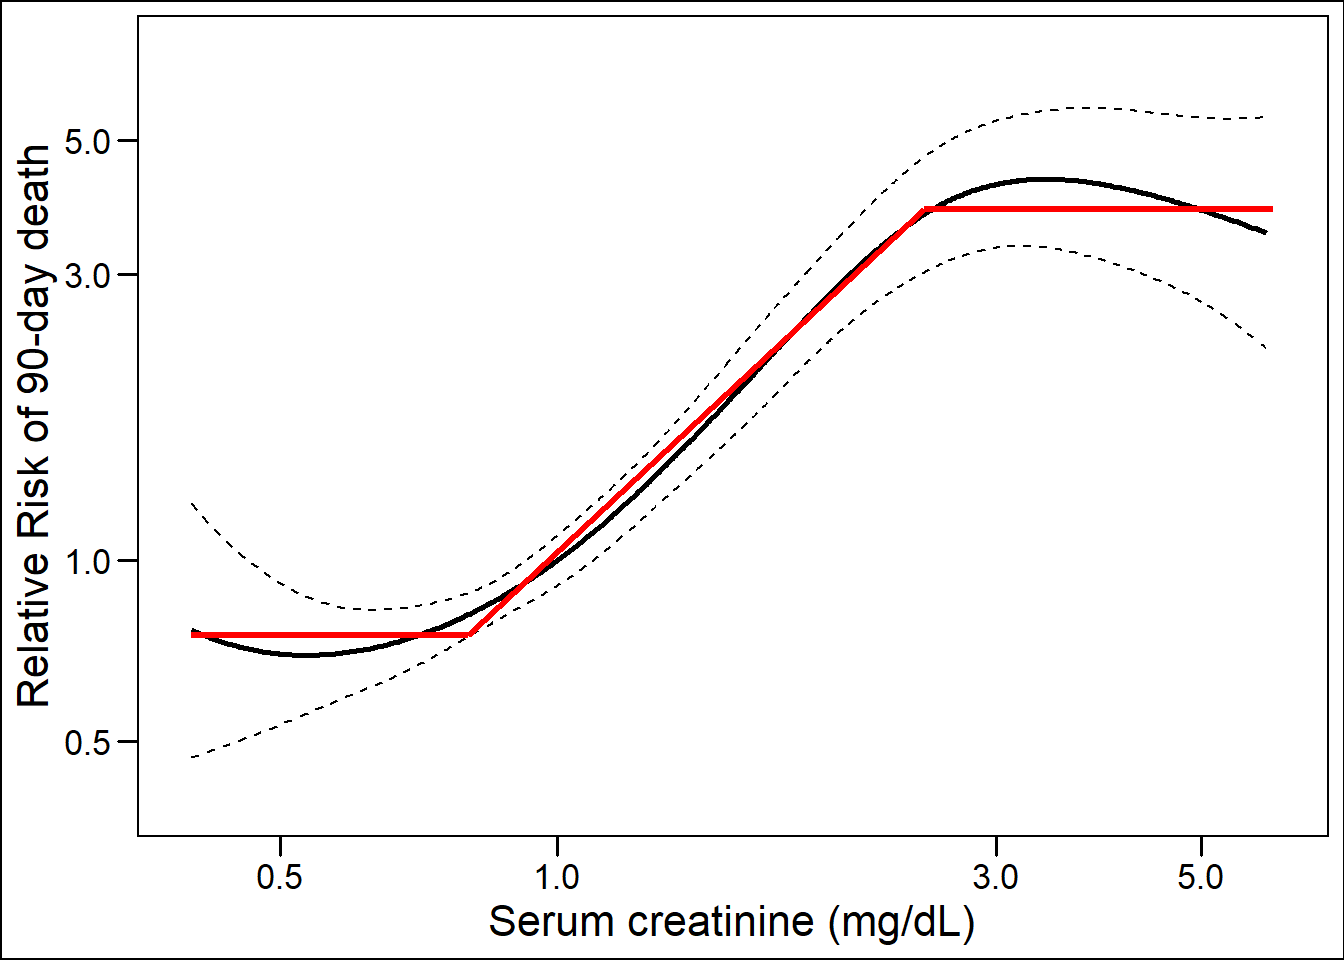
\includegraphics[height=0.27\textheight]{thesis_files/figure-latex/refit-fig2-1} }\newline\subfloat[Bilirubin\label{fig:refit-fig2-2}]{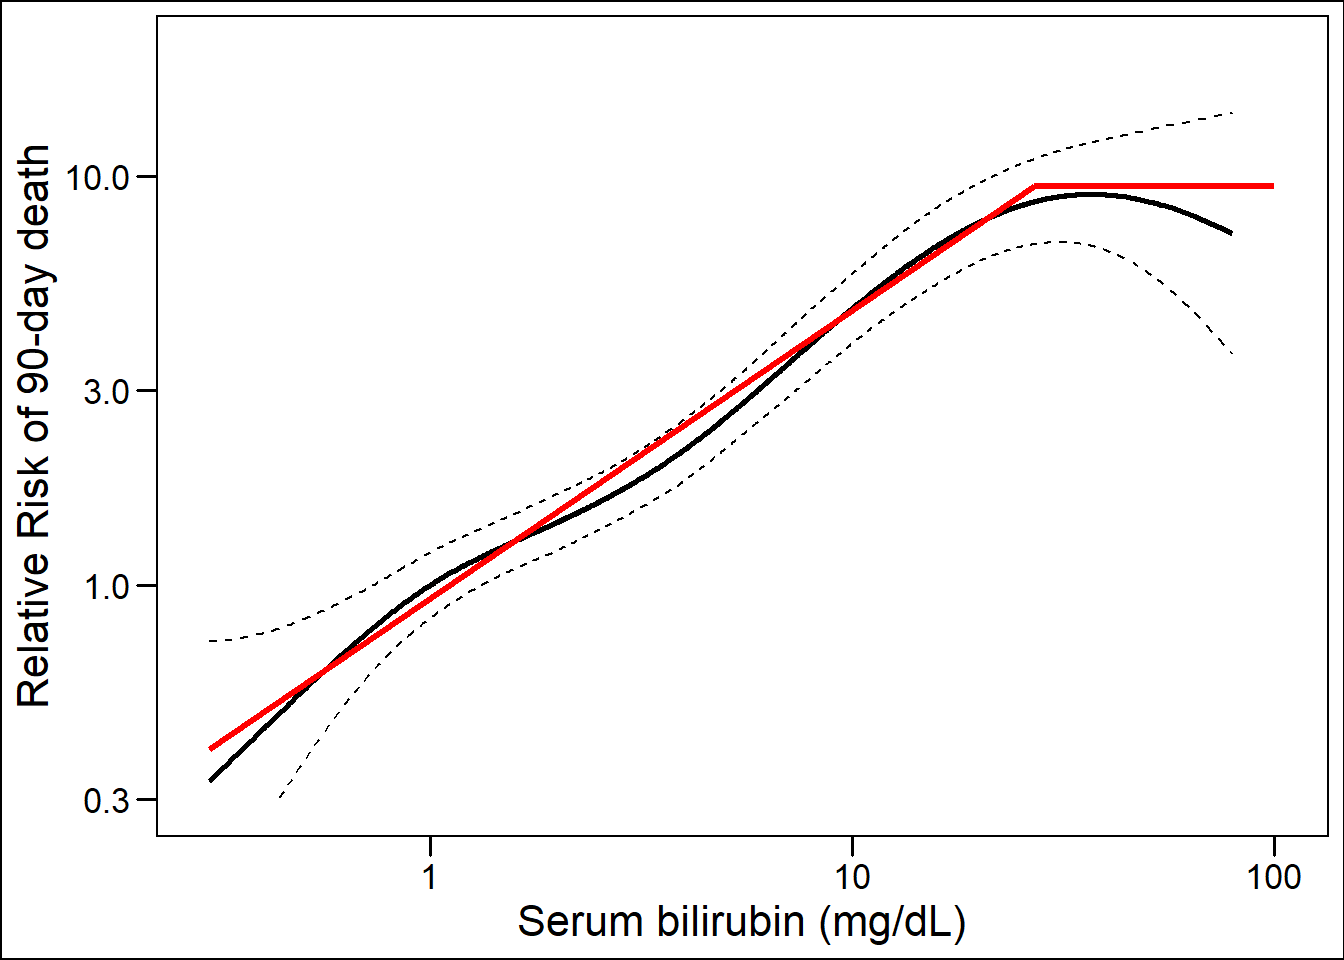
\includegraphics[height=0.27\textheight]{thesis_files/figure-latex/refit-fig2-2} }\newline\subfloat[INR\label{fig:refit-fig2-3}]{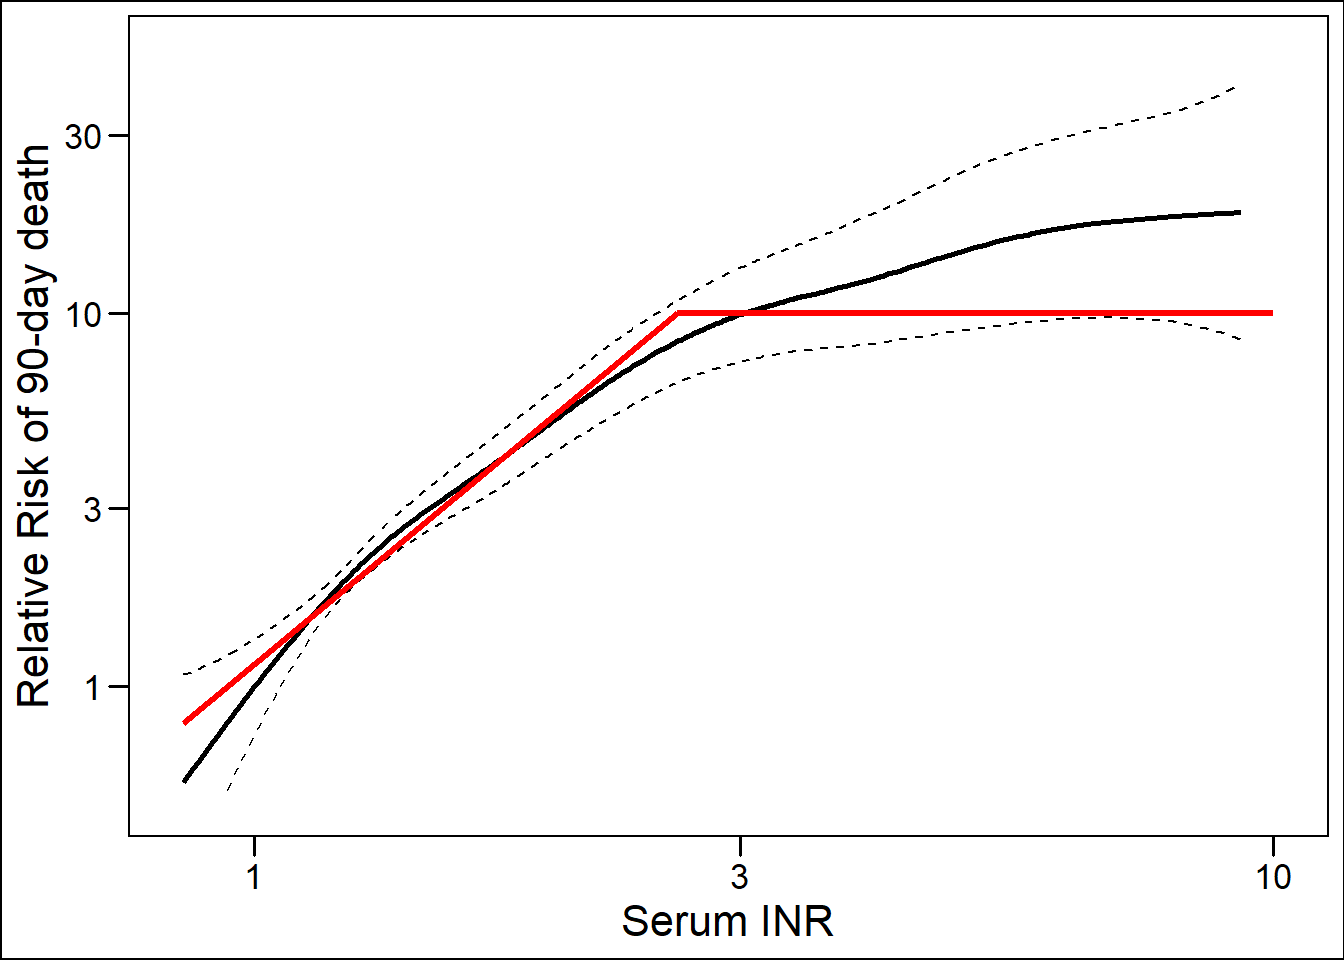
\includegraphics[height=0.27\textheight]{thesis_files/figure-latex/refit-fig2-3} }

}

\caption{For each parameter, the diagonal line represent the coefficient (slope of the diagonal) and lower and upper boundaries (horizontal segments) in refit MELD}\label{fig:refit-fig2}
\end{figure}

The heatmaps of the calculated log-likelihoods and c-indices per combination of boundaries are attached in the (online) supplement. After checking for interactions and matching the 25th and 75th quantiles of the reMELD to the UNOS-MELD in the training data, the reMELD equation was: \[7.728*ln(creatinine) + 3.446*ln(bilirubin) + 10.597*ln(INR) + 8.422\] In this equation the abovementioned boundaries were used for the parameters.
The maximum log-likelihood for Na levels was found between 120 and 139 mmol/L. Combining the reMELD and Na showed a significant interaction between Na and creatinine. Thus, after quantile matching in the training data, the reMELD-Na formula was:
\begin{align*} 
\ 9.025\times ln(creatinine) + 2.969\times ln(bilirubin) + 9.518\times ln(INR) -\\ 
\ 0.392\times (139-Na) - 0.351\times ln(139-Na)\times ln(creatinine)
\end{align*}

\begin{table}

\caption{\label{tab:refit-tab2}Parameter bounds and number of patient measurements included in UNOS and refit models}
\centering
\resizebox{\linewidth}{!}{
\begin{threeparttable}
\begin{tabular}[t]{llllllll}
\toprule
\multicolumn{2}{c}{ } & \multicolumn{3}{c}{UNOS MELD(-Na)} & \multicolumn{3}{c}{refit MELD(-Na)} \\
\cmidrule(l{3pt}r{3pt}){3-5} \cmidrule(l{3pt}r{3pt}){6-8}
 &  & bounds & capped (\%) & included (\%) & bounds & capped (\%) & included (\%)\\
\midrule
\cellcolor{gray!6}{Creatinine} & \cellcolor{gray!6}{lower} & \cellcolor{gray!6}{1} & \cellcolor{gray!6}{55.0} & \cellcolor{gray!6}{41.9} & \cellcolor{gray!6}{0.7} & \cellcolor{gray!6}{20.1} & \cellcolor{gray!6}{73}\\
 & upper & 4 & 3.1 &  & 2.5 & 6.9 & \\
\cellcolor{gray!6}{Bilirubin} & \cellcolor{gray!6}{lower} & \cellcolor{gray!6}{1} & \cellcolor{gray!6}{23.7} & \cellcolor{gray!6}{76.3} & \cellcolor{gray!6}{0.3} & \cellcolor{gray!6}{2.0} & \cellcolor{gray!6}{93.5}\\
 & upper & NA &  &  & 26.9 & 4.5 & \\
\cellcolor{gray!6}{INR} & \cellcolor{gray!6}{lower} & \cellcolor{gray!6}{1} & \cellcolor{gray!6}{9.8} & \cellcolor{gray!6}{91.2} & \cellcolor{gray!6}{0.1} & \cellcolor{gray!6}{NA} & \cellcolor{gray!6}{94.8}\\
 & upper & NA &  &  & 2.6 & 5.2 & \\
\cellcolor{gray!6}{Sodium} & \cellcolor{gray!6}{lower} & \cellcolor{gray!6}{125} & \cellcolor{gray!6}{2.7} & \cellcolor{gray!6}{72.9} & \cellcolor{gray!6}{120} & \cellcolor{gray!6}{0.7} & \cellcolor{gray!6}{56.3}\\
 & upper & 140 & 24.4 &  & 138.6 & 43 & \\
\bottomrule
\end{tabular}
\begin{tablenotes}
\item \textit{Note: } 
\item For each parameter the lower and upper bounds are shown. 'capped' shows the percentage of the cohort that either lies under or above the chosen bounds. 'included' shows the percentage of patients whose measurements are included in the model.
\end{tablenotes}
\end{threeparttable}}
\end{table}

For the parameters in the reMELD-Na score, the abovementioned boundaries were used. Compared to the UNOS-MELD, re-MELD and reMELD-Na used respectively 149\% (n=4815) and 42\% (n=2748) more patient measurements, i.e.~less true patient measurements were capped, at listing with the boundaries as shown in Table \ref{tab:refit-tab2}.

\begin{figure}

{\centering \subfloat[Creatinine\label{fig:refit-fig3-1}]{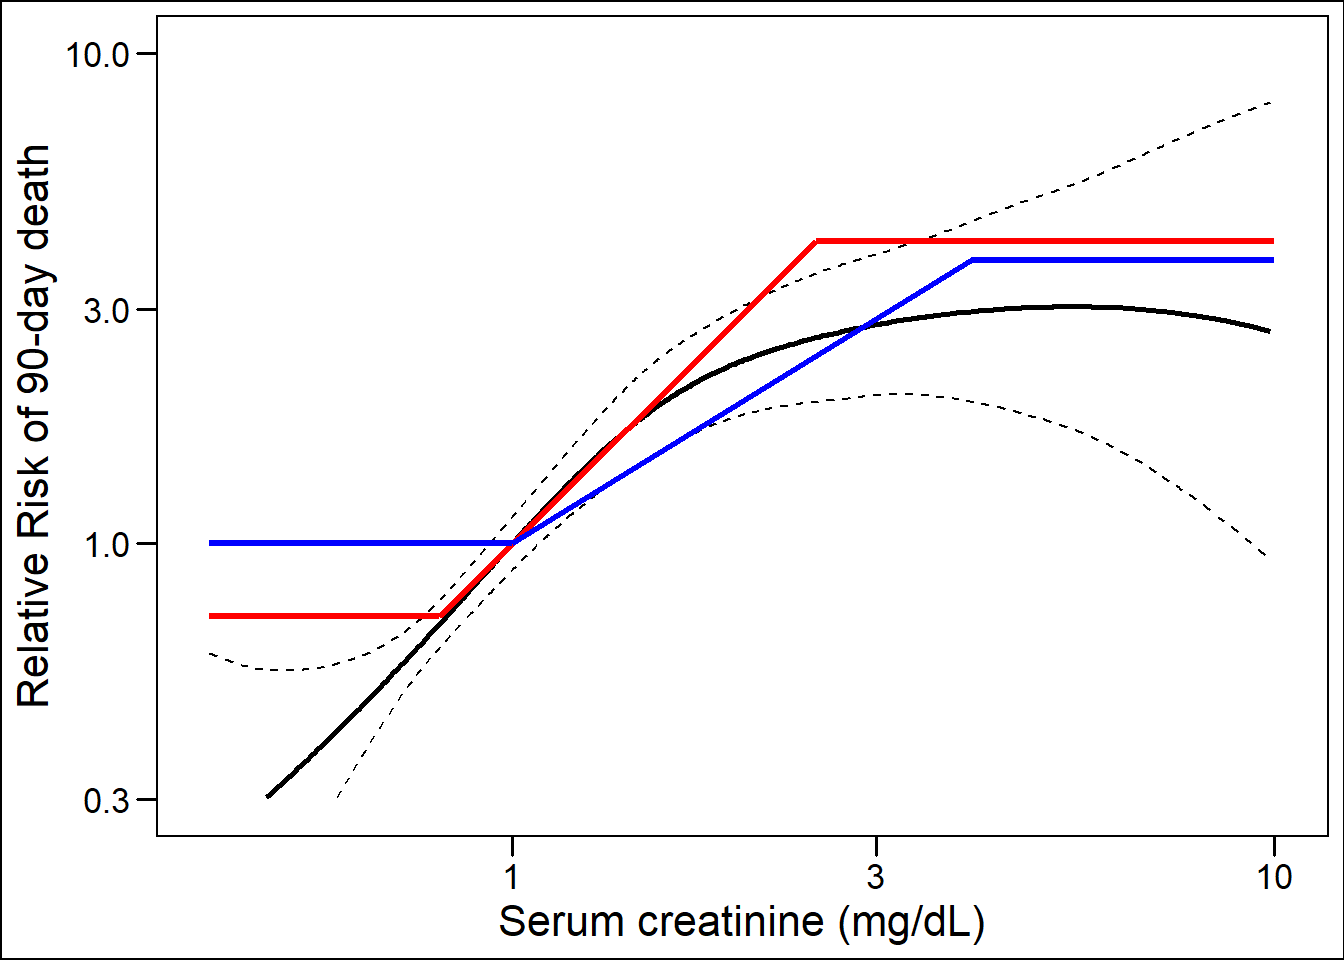
\includegraphics[height=0.27\textheight]{thesis_files/figure-latex/refit-fig3-1} }\newline\subfloat[Bilirubin\label{fig:refit-fig3-2}]{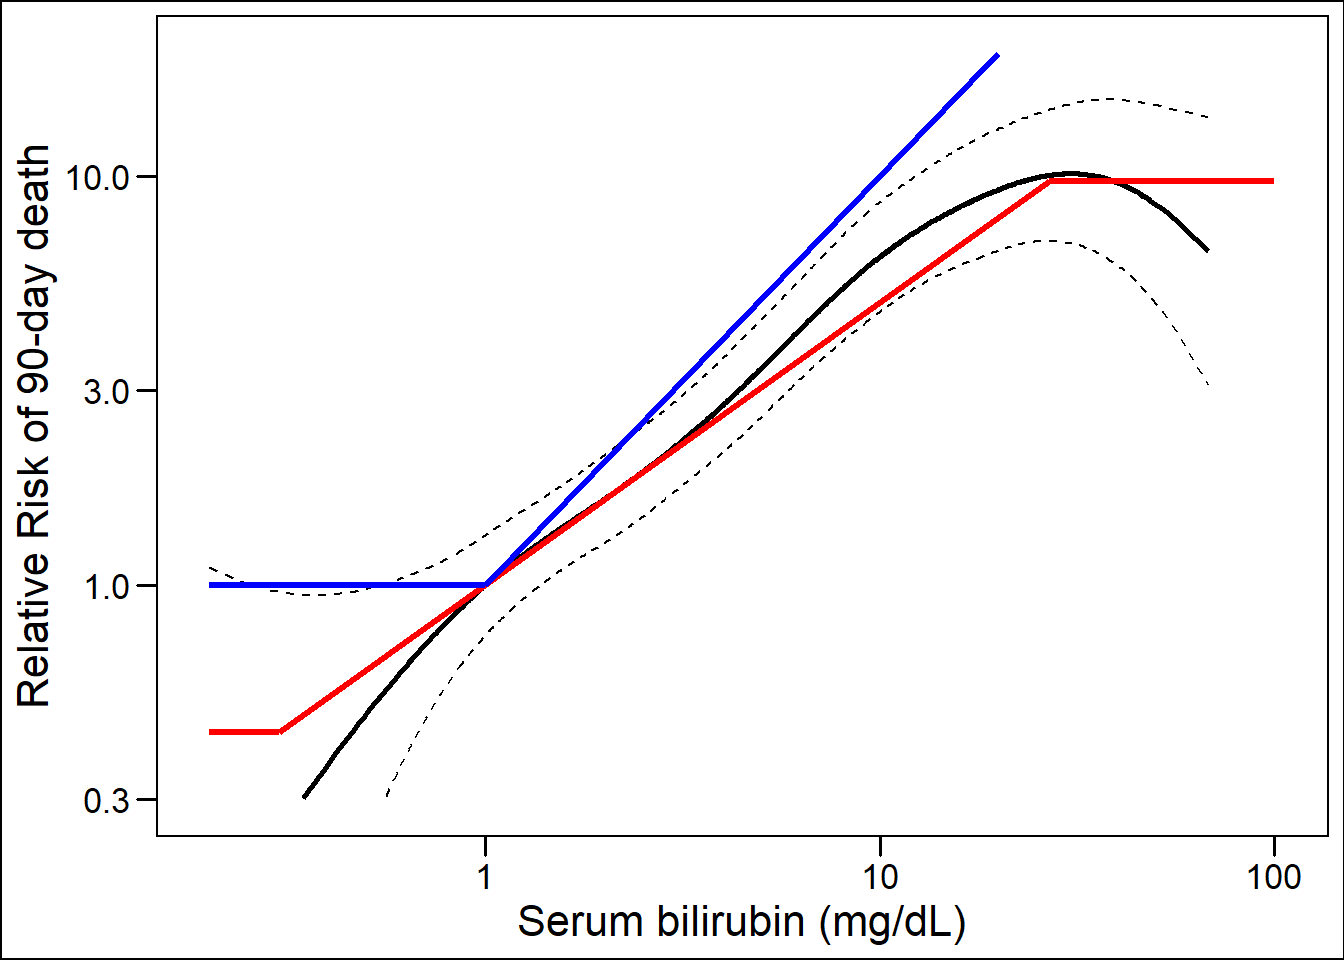
\includegraphics[height=0.27\textheight]{thesis_files/figure-latex/refit-fig3-2} }\newline\subfloat[INR\label{fig:refit-fig3-3}]{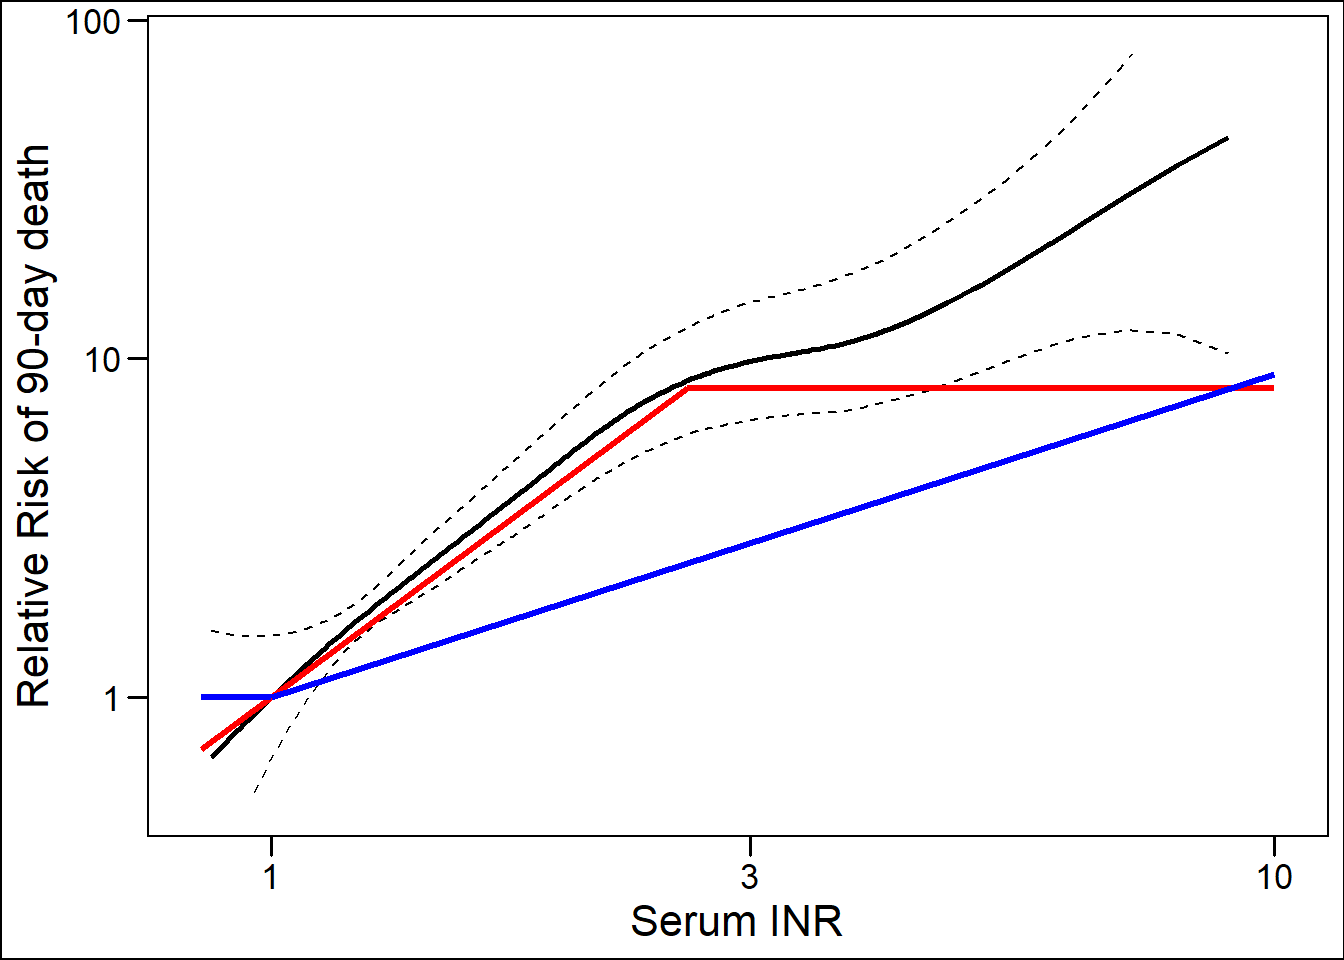
\includegraphics[height=0.27\textheight]{thesis_files/figure-latex/refit-fig3-3} }

}

\caption{In the validation data, the relation with 90-day mortality is shown. The coefficients and boundaries of creatinine in reMELD (red) and UNOS-MELD (blue) illustrate model fit.}\label{fig:refit-fig3}
\end{figure}

\hypertarget{model-performance}{%
\subsection*{Model performance}\label{model-performance}}
\addcontentsline{toc}{subsection}{Model performance}

Figure \ref{fig:refit-fig3} shows the effect of each MELD parameter, corrected for the others, on 90-day mortality in the validation data. The red and blue lines represent the coefficients of the reMELD and UNOS-MELD respectively. It was visually apparent that refit MELD showed a better fit to the data for all three parameters. The calculated chi-square values confirmed significant (p\textless0.001) improvements in the refit models compared to the UNOS-MELD, shown in Table \ref{tab:refit-tab3}. The reMELD and reMELD-Na models showed c-indices of 0.866 and 0.869 respectively, which were significantly (p\textless0.001) higher than 0.849 of the UNOS-MELD, see Table \ref{tab:refit-tab3}. Furthermore, the reMELD-Na showed a 8\% reduction in prediction error as compared to UNOS-MELD with Brier scores of 0.053 (reMELD-Na) and 0.057 (UNOS-MELD) respectively.

\begin{table}

\caption{\label{tab:refit-tab3}Comparison of models in validation data}
\centering
\resizebox{\linewidth}{!}{
\begin{threeparttable}
\begin{tabular}[t]{llrrl}
\toprule
Model & C-index & Max log-likelihood & Chisq & p\\
\midrule
\cellcolor{gray!6}{UNOS MELD} & \cellcolor{gray!6}{0.849  (se = 0.012 )} & \cellcolor{gray!6}{-1376.6} & \cellcolor{gray!6}{} & \cellcolor{gray!6}{}\\
UNOS MELD-Na & 0.860  (se = 0.010 ) & -1362.8 & 27.660 & < 2.2e-16\\
\cellcolor{gray!6}{reMELD} & \cellcolor{gray!6}{0.866  (se = 0.011 )} & \cellcolor{gray!6}{-1347.1} & \cellcolor{gray!6}{58.966} & \cellcolor{gray!6}{< 2.2e-16}\\
reMELD-Na & 0.869  (se = 0.010 ) & -1347.1 & 59.066 & < 2.2e-16\\
\bottomrule
\end{tabular}
\begin{tablenotes}
\item \textit{Note: } 
\item For each model the C- index and maximum log- likelihood are calculated in the validation data. The likelihood ratio comparisons of the models to UNOS- MELD are shown by chi- squared and P values.
\end{tablenotes}
\end{threeparttable}}
\end{table}

\hypertarget{impact-on-the-waiting-list-1}{%
\subsection*{Impact on the waiting list}\label{impact-on-the-waiting-list-1}}
\addcontentsline{toc}{subsection}{Impact on the waiting list}

After 90 days of follow-up, 1,248 patients of our cohort were transplanted. By using the reMELD-Na compared to the UNOS-MELD to allocate the 1,248 available liver grafts, 134/1,248 (11.5\%) of the transplanted patients would have been within the top 1,248 candidates under one of these models but not under the other; i.e., prioritization would differ. Table \ref{tab:refit-tab4} shows the characteristics of these differently prioritized patients. Most notably, reMELD-Na-prioritized patients were slightly older, were more often male, and had a higher prevalence of cirrhosis. Unsurprisingly, these patients had significantly lower serum sodium levels (138 vs.~127 mmol/L). As hyponatremia is most often seen in alcohol-associated cirrhosis,\textsuperscript{14} the sex and age differences are largely explained.
The correlation plot Figure \ref{fig:refit-fig4} shows which patients would be prioritized according to either UNOS-MELD or re-MELD-Na allocation.

\linespread{1}

\begin{landscape}\begin{table}

\caption{\label{tab:refit-tab4}Characteristics of Prioritized Patients}
\centering
\resizebox{\linewidth}{!}{
\begin{tabular}[t]{llllll}
\toprule
Characteristics & Transplanted both & UNOS MELD Transplanted & reMELD-Na Transplanted & Not transplanted & p\\
\midrule
\cellcolor{gray!6}{n} & \cellcolor{gray!6}{1105} & \cellcolor{gray!6}{143} & \cellcolor{gray!6}{143} & \cellcolor{gray!6}{5553} & \cellcolor{gray!6}{}\\
Age at listing (mean (SD)) & 53.42 (10.48) & 48.73 (13.62) & 55.29 (9.53) & 54.09 (10.77) & <0.001\\
\cellcolor{gray!6}{Gender female (\%)} & \cellcolor{gray!6}{362 ( 32.8)} & \cellcolor{gray!6}{66 ( 46.2)} & \cellcolor{gray!6}{44 ( 30.8)} & \cellcolor{gray!6}{1750 ( 31.5)} & \cellcolor{gray!6}{0.003}\\
Length (mean (SD)) & 172.87 (10.88) & 171.73 (8.85) & 173.59 (10.16) & 173.03 (9.56) & 0.368\\
\cellcolor{gray!6}{Weight (mean (SD))} & \cellcolor{gray!6}{81.42 (18.43)} & \cellcolor{gray!6}{77.33 (18.19)} & \cellcolor{gray!6}{79.30 (18.30)} & \cellcolor{gray!6}{79.03 (17.41)} & \cellcolor{gray!6}{<0.001}\\
\addlinespace[0.3em]
\multicolumn{6}{l}{\textbf{Disease (\%)}}\\
\hspace{1em}Cirrhosis, Alcoholic & 390 ( 35.3) & 48 ( 33.6) & 65 ( 45.5) & 1458 ( 26.3) & \\
\hspace{1em}\cellcolor{gray!6}{Cirrhosis, HCV} & \cellcolor{gray!6}{74 (  6.7)} & \cellcolor{gray!6}{6 (  4.2)} & \cellcolor{gray!6}{10 (  7.0)} & \cellcolor{gray!6}{385 (  6.9)} & \cellcolor{gray!6}{}\\
\hspace{1em}Cirrhosis, other causes & 285 (25.8) & 27 (18.9) & 33 (23.1) & 833 (15.0) & \\
\hspace{1em}\cellcolor{gray!6}{Cholestatic disease} & \cellcolor{gray!6}{113 (10.2)} & \cellcolor{gray!6}{15 (10.5)} & \cellcolor{gray!6}{7 (4.90)} & \cellcolor{gray!6}{811 (14.6)} & \cellcolor{gray!6}{}\\
\hspace{1em}HCC and cirrhosis & 37 (  3.3) & 3 (  2.1) & 9 (  6.3) & 1325 ( 23.9) & \\
\hspace{1em}\cellcolor{gray!6}{Other} & \cellcolor{gray!6}{207 (18.7)} & \cellcolor{gray!6}{44 (30.7)} & \cellcolor{gray!6}{19 (13.2)} & \cellcolor{gray!6}{739 (13.3)} & \cellcolor{gray!6}{}\\
\addlinespace[0.3em]
\multicolumn{6}{l}{\textbf{Status after 90 days}}\\
\hspace{1em}Censored due to HU or NSE & 52 (  4.7) & 9 (  6.3) & 8 (  5.6) & 1578 ( 28.5) & \\
\hspace{1em}\cellcolor{gray!6}{Deceased} & \cellcolor{gray!6}{338 (  30.7)} & \cellcolor{gray!6}{28 (  19.6)} & \cellcolor{gray!6}{36 ( 25.2)} & \cellcolor{gray!6}{276 (  5.0)} & \cellcolor{gray!6}{}\\
\hspace{1em}Removed from the list & 121 ( 11.0) & 30 ( 21.0) & 27 ( 18.9) & 703 ( 12.7) & \\
\hspace{1em}\cellcolor{gray!6}{Still waiting on waiting list} & \cellcolor{gray!6}{56 (  5.1)} & \cellcolor{gray!6}{19 ( 13.3)} & \cellcolor{gray!6}{28 ( 19.6)} & \cellcolor{gray!6}{2370 ( 42.8)} & \cellcolor{gray!6}{}\\
\hspace{1em}Transplanted & 536 ( 48.6) & 57 ( 39.9) & 44 ( 30.8) & 611 ( 11.0) & \\
\cellcolor{gray!6}{Days listed (mean (SD))} & \cellcolor{gray!6}{24.94 (78.46)} & \cellcolor{gray!6}{51.32 (114.64)} & \cellcolor{gray!6}{72.64 (132.97)} & \cellcolor{gray!6}{175.21 (304.96)} & \cellcolor{gray!6}{<0.001}\\
\addlinespace[0.3em]
\multicolumn{6}{l}{\textbf{Measurement at listing (mean (SD))}}\\
\hspace{1em}Creatinine in mg/dL & 2.95 (8.51) & 2.67 (9.43) & 1.26 (0.48) & 1.09 (1.18) & <0.001\\
\hspace{1em}\cellcolor{gray!6}{Bilirubin in mg/dL} & \cellcolor{gray!6}{19.29 (14.10)} & \cellcolor{gray!6}{10.69 (9.08)} & \cellcolor{gray!6}{8.01 (5.96)} & \cellcolor{gray!6}{2.89 (3.51)} & \cellcolor{gray!6}{<0.001}\\
\hspace{1em}INR & 2.43 (1.20) & 2.37 (1.40) & 1.74 (0.32) & 1.30 (0.28) & <0.001\\
\hspace{1em}\cellcolor{gray!6}{Sodium in mmol/L} & \cellcolor{gray!6}{134.26 (6.08)} & \cellcolor{gray!6}{138.21 (4.67)} & \cellcolor{gray!6}{127.34 (5.34)} & \cellcolor{gray!6}{137.76 (4.20)} & \cellcolor{gray!6}{<0.001}\\
(refit)MELD score & 30.95 (5.48) & 25.57 (2.95) & 21.10 (2.26) & 12.91 (4.60) & <0.001\\
\cellcolor{gray!6}{Dialysis dependent (\%)} & \cellcolor{gray!6}{165 ( 15.3)} & \cellcolor{gray!6}{21 ( 15.1)} & \cellcolor{gray!6}{0 (  0.0)} & \cellcolor{gray!6}{87 (  1.6)} & \cellcolor{gray!6}{<0.001}\\
\bottomrule
\end{tabular}}
\end{table}
\end{landscape}

\linespread{1.213}

\begin{figure}[!h]

{\centering 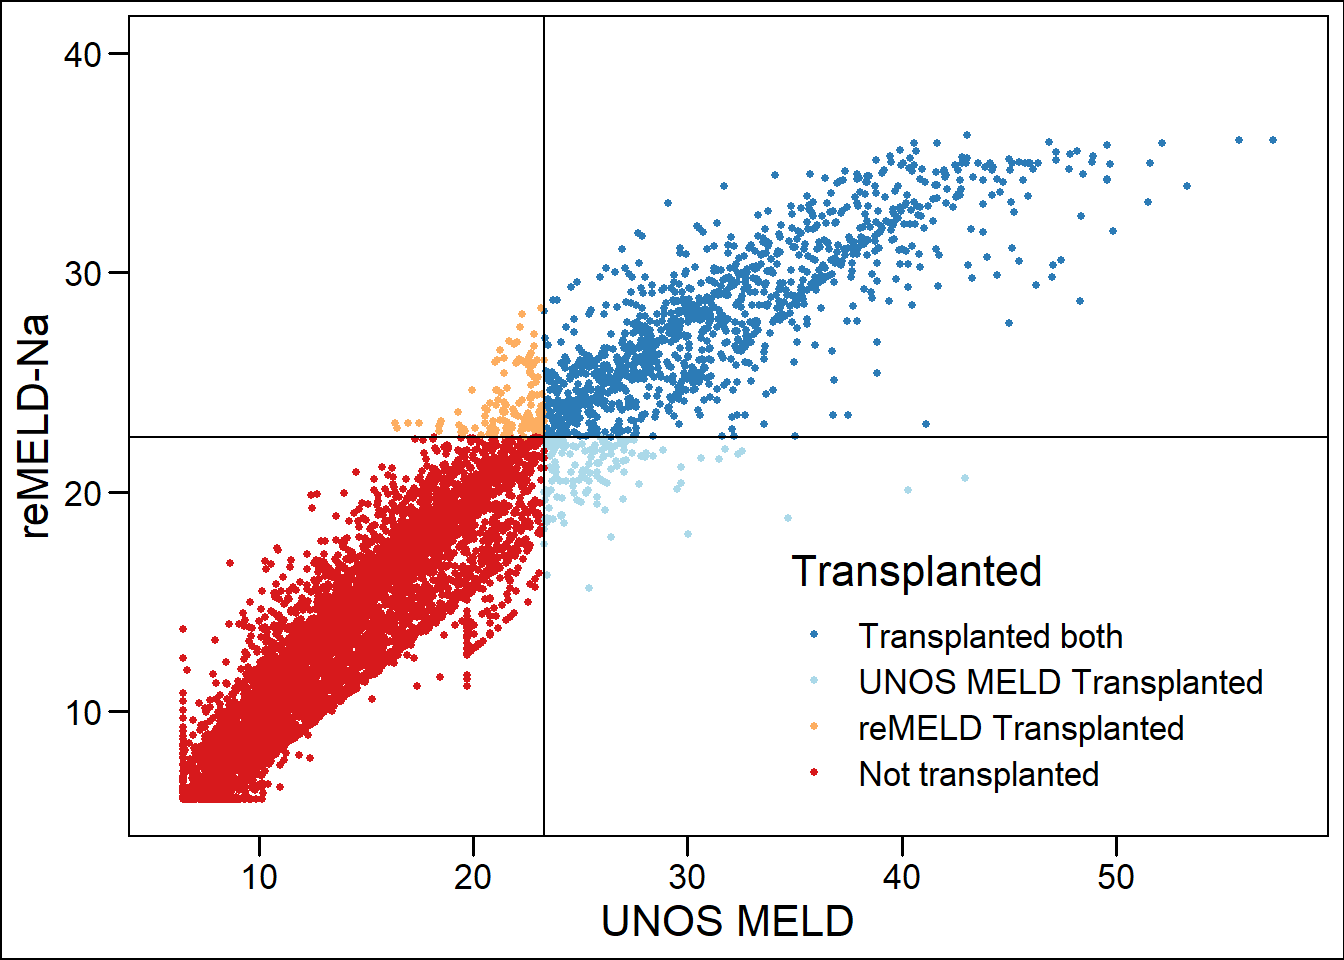
\includegraphics{thesis_files/figure-latex/refit-fig4-1} 

}

\caption{Correlation plot of UNOS- MELD and reMELD- Na. Based on the number of transplanted patients after the first 90 days (n = 1,248), the highest- ranked patients according to both scores separately were assigned a liver graft, as represented by the horizontal (graft granted by reMELD- Na) and vertical (by UNOS- MELD) lines. Patients in the top left quadrant (reMELD- Na- prioritized) had a 1.58 times higher risk of 90- day death compared to patients in the lower right quadrant (UNOS- MELD- prioritized).}\label{fig:refit-fig4}
\end{figure}

The patients in the top left quadrant would have been prioritized by reMELD-Na allocation but not by UNOS-MELD. They had estimated 90-day survival probabilities of 52.4\% (95CI 41.3 -- 66.5), as compared to 70.0\% (95CI 58.9 -- 83.1) for patients prioritized by UNOS-MELD, but not by reMELD-Na (bottom right quadrant), Thus, re-MELD-Na would have prioritized patients with a 90-day WL mortality HR of 1.6 as compared to currently prioritized patients. Figure \ref{fig:refit-fig4} also illustrated that after refitting, no scores above 40 were calculated and thus that all high MELD scores were acknowledged correctly. By using more recent data and the true 90-day mortality rates of our population, reMELD-Na showed that very few patients actually approached 100\% 90-day WL mortality, i.e.~MELD 40. Thus, the refit models restored the clinical meaning of the 6-40-point range.

\hypertarget{discussion-1}{%
\section*{Discussion}\label{discussion-1}}
\addcontentsline{toc}{section}{Discussion}

In this study, for the first time the MELD score was refitted to the Eurotransplant data. By establishing new and evidence-based lower and upper bounds for each MELD parameter, the role of each MELD component was reweighed. The reweighed coefficients performed significantly better than the currently used UNOS-MELD in the independent validation dataset. The reMELD and reMELD-Na gave convincingly higher c-indices than UNOS-MELD and were based on the best fit to the current Eurotransplant data. The reMELD-Na prioritized patients with 1.6 times higher 90-day mortality rates than the currently prioritized patients. Thus, refitting MELD results in more accurate, effective and just mortality prediction and subsequent sickest-first allocation.

The UNOS-MELD has remained unchanged ever since it was constructed 20 years ago in a cohort of 231 patients.\textsuperscript{4} Its parameter bounds were chosen arbitrarily.\textsuperscript{5,6,11} Thus, UNOS-MELD is not fit for the changing LT candidate population, which showed through a decline in predictive power.\textsuperscript{7} Refitting, i.e.~re-establishing parameter bounds and weights, enables prediction models to change along with the population they serve. Indeed, the principle of refitting could be applied to any model used for survival prediction.

\hypertarget{lower-bounds}{%
\subsection*{Lower bounds}\label{lower-bounds}}
\addcontentsline{toc}{subsection}{Lower bounds}

By refitting, the lower border of creatinine was set to 0.7. A creatinine of 1.0 mg/dL might already indicate disease in LT candidates, as measured creatinine overestimates kidney function in e.g.~sarcopenia, females and patients with high bilirubin.\textsuperscript{15} Evaluation of the lower bounds of bilirubin and the INR showed that multiple combinations of bounds provided a good fit to the data, while preserving the predictive power of the model. Thus, the exact lower bounds should be determined through expert-based discussion. By acknowledging more low values (which most patients had at listing), the higher values were placed in a more appropriate context than with the UNOS lower bounds of 1.0.

\hypertarget{upper-bounds}{%
\subsection*{Upper bounds}\label{upper-bounds}}
\addcontentsline{toc}{subsection}{Upper bounds}

The upper bounds found in this study were perhaps more controversial, as UNOS-MELD uses none for bilirubin and INR. However, the new bounds resulted in better-performing models. Through refitting, serum creatinine became less important. Under UNOS-MELD, the number of transplanted patients with renal failure increased significantly, possibly due to overweighed creatinine in UNOS-MELD.\textsuperscript{6,16} As these patients have increased morbidity and mortality both before and after LT, the principle of the sickest-first system was to prioritize them. However, one could question the prioritization of renal failure above liver failure, through the high weight of creatinine in UNOS-MELD, when allocating scarce liver grafts.
High bilirubin levels led to unreliable measurements of UNOS-MELD due to interaction with creatinine, which influenced scores because of the weight of creatinine in UNOS-MELD.\textsuperscript{17} Therefore, decreasing the weight of creatinine and establishing an upper bound for bilirubin should give more reliable reMELD scores. Of the three MELD parameters, INR is the most unreliable. This is in part because the INR varies significantly depending on the method of laboratory measurement.\textsuperscript{18} Also, medical treatment (or non-treatment) can decrease or increase the INR. Therefore, an upper bound for the INR would also be an improvement, as it would reduce the influence of outliers in INR measurements.\textsuperscript{5}

\hypertarget{sodium-addition}{%
\subsection*{Sodium addition}\label{sodium-addition}}
\addcontentsline{toc}{subsection}{Sodium addition}

The UNOS regions have used MELD-Na for liver allocation since 2016.\textsuperscript{3} Despite the proven impact of serum sodium levels on LT candidate survival,\textsuperscript{12,14} Na is not used (yet) for the Eurotransplant liver allocation. The addition of Na to the reMELD gave a small but significant improvement in discriminative ability (c-index 0.866 to 0.869). Although the largest improvement in c-index was achieved by reMELD alone (0.849 to 0.866), the additional smaller gain still represented important changes for hyponatremic patients. The c-index measures the proportion of patient pairs whose ranking is correctly ordered. Hence, a difference in c-index can be thought of as the proportion of patients whose ranking change. It however does not measure the degree of change within ranks, i.e.~for each patient. Thus, a small difference for many patients will give a high c-index increase, whereas a large change for a smaller number of (hyponatremic) patients gives little improvement.\textsuperscript{12,14} Based on the current findings, reMELD-Na performed slightly but significantly better than reMELD. Also, it seems just to consider the proven effect of Na levels on mortality. Therefore, use of reMELD-Na is preferred.

\hypertarget{impact-on-the-wl}{%
\subsection*{Impact on the WL}\label{impact-on-the-wl}}
\addcontentsline{toc}{subsection}{Impact on the WL}

Despite the seemingly small performance differences between UNOS and refit models, the refit models were very different at their bases, which was the goal of this study. Refitting established new parameter bounds, notably different coefficients and a superior fit to the data, see Figure \ref{fig:refit-fig3} and Table \ref{tab:refit-tab3}. This improved both model discrimination (c-index) and calibration (prediction errors). The increase in c-index from 0.849 to 0.869 may seem small, but is both statistically and clinically very significant. Recent study showed that switching from UNOS MELD to MELD-Na would significantly reduce waiting list mortality in the Eurotransplant region, although the difference in c-index was 0.015 (0.832 vs 0.847).\textsuperscript{14} The study that formed the basis of the US switch from MELD to MELD-Na, showed a similar increase in c-index (i.e.~0.868 to 0.883),\textsuperscript{12} which was considered an important increase and convincing evidence for possible MELD-Na implementation. Another large UNOS cohort study on improving MELD showed a c-index increase from 0.75 to 0.77.\textsuperscript{16} This illustrates that improving an already-high c-index is very difficult, as it increases in an asymptotic fashion when approaching its maximum. The highest obtainable baseline c-index is probably around 0.9 or lower because of possible imperfections and biological variation in the data.\textsuperscript{5,12,14} Moreover, compared to respectively UNOS MELD and MELD-Na, refitting reduced prediction errors by 8\% and 5\%, which is a major improvement considering the already-high accuracy of the scores.

To estimate the possible clinical impact of refitting, differences in prioritization were assessed, see Table \ref{tab:refit-tab4}. As the 90-day mortality of the reMELD-Na-prioritized patients (Figure \ref{fig:refit-fig4} ) was 1.6 times higher than the currently prioritized patients, reMELD-Na could possibly better effectuate the sickest-first principle. Figure \ref{fig:refit-fig4} also shows patients with MELD\textgreater=40, which were rescaled below 40 after refitting. An UNOS-MELD score of 40 originally corresponded to a 100\% 90-day WL mortality.\textsuperscript{11} However, over the past decades, the waitlist population and the risks of death per MELD score have changed,\textsuperscript{7} which also shows through the increasing number and survival of MELD\textgreater=40 patients.\textsuperscript{19} This has important implications for the Eurotransplant exception point system, which is based on MELD mortality rates dating from 2006 (supplement 3) and allocates 25-30\% of the LT candidates.\textsuperscript{10,20} Regardless of possible refit score implementation, the Eurotransplant exception point system would benefit from an accurate rescaling. Still, by quantile matching and refitting specifically in the 6 to 40 range, the refit scores restored their old mortality equivalents, i.e.~MELD 40 represented a 100\% 90-day mortality risk.

\hypertarget{limitations-1}{%
\subsection*{Limitations}\label{limitations-1}}
\addcontentsline{toc}{subsection}{Limitations}

Estimating the impact of a new allocation system based on another system's data inadequately reflects the possible effects of new allocation. Before implementation, one aims to answer important questions concerning counterfactual outcomes in causal inference, e.g.~what would have happened to patients had they not been transplanted. The best way to evaluate a new allocation system is to bring it in practice and measure the difference. Evaluating a new system through simulation is probably the next best option. One should be aware, however, that assessment through simulation is based on intrinsically unverifiable assumptions, namely that with changing the allocation priorities nothing else in the system will change. The Eurotransplant region does not yet have a simulation model of its liver allocation, like the Liver Simulation Allocation Model (LSAM) in the UNOS. Therefore, new allocation systems, e.g.~refit models, cannot be formally evaluated before possible implementation. Instead, only a rough estimate of possible impact could be given by assessing differences in prioritized patients. Still, this was likely a less-biased method compared to proposed UNOS MELD-Na estimations of impact.\textsuperscript{12}

Finally, the role of clinical intuition and logic of reasoning should not be underestimated. Optimizing MELD for our region makes clinical sense and the log-likelihood-based approach is statistically solid and logical. Regions without simulation programs cannot know for certain what the effect of new allocation systems will be. Still, evidence can form a strong suggestion of improvement, which can be confirmed after possible implementation.

\hypertarget{conclusion-1}{%
\section*{Conclusion}\label{conclusion-1}}
\addcontentsline{toc}{section}{Conclusion}

This study showed that updating the boundaries and coefficients on more recent region-specific data increased the predictive power of MELD again. The discussion on the establishment of refit models should consider at least three aspects: the parameter boundaries, fit of the model to the data and the prediction performance of the model. With the increasing interest in more advanced computational possibilities, the transplant community should investigate alternative models to the current allocation system.\textsuperscript{21} However, as the MELD still is the basis of liver allocation in many regions, efforts should be made to keep the model as relevant as possible, and we believe the current study serves this purpose. In conclusion, refitting MELD acknowledged more patient measurements at listing and prioritized patients with higher 90-day mortality. The discriminative ability and accuracy of refit models was a significant and relevant improvement compared to the currently used UNOS-MELD.

\newpage
\linespread{1}
\small

\hypertarget{references-2}{%
\section*{References}\label{references-2}}
\addcontentsline{toc}{section}{References}

\begin{enumerate}
\def\labelenumi{\arabic{enumi}.}
\tightlist
\item
  Eurotransplant International Foundation. Statistics Library.
\item
  Kamath PS, Wiesner RH, Malinchoc M, et al.~A model to predict survival in patients with end-stage liver disease. Hepatology. 2001;33(2):464-470. \url{doi:10.1053/jhep.2001.22172}
\item
  OPTN. Organ procurement and transplantation network policies.
\item
  Malinchoc M, Kamath PS, Gordon FD, Peine CJ, Rank J, Ter Borg PCJ. A model to predict poor survival in patients undergoing transjugular intrahepatic portosystemic shunts. Hepatology. 2000;31(4):864-871. \url{doi:10.1053/he.2000.5852}
\item
  Leise MD, Kim WR, Kremers WK, Larson JJ, Benson JT, Therneau TM. A revised model for end-stage liver disease optimizes prediction of mortality among patients awaiting liver transplantation. Gastroenterology. 2011;140(7):1952-1960. \url{doi:10.1053/j.gastro.2011.02.017}
\item
  Merion RM, Sharma P, Mathur AK, Schaubel DE. Evidence-based development of liver allocation: A review. Transpl Int. 2011;24(10):965-972. \url{doi:10.1111/j.1432-2277.2011.01274.x}
\item
  Godfrey EL, Malik TH, Lai JC, et al.~The decreasing predictive power of MELD in an era of changing etiology of liver disease. Am J Transplant. 2019;19(12):3299-3307. \url{doi:10.1111/ajt.15559}
\item
  Nagai S, Chau LC, Schilke RE, et al.~Effects of Allocating Livers for Transplantation Based on Model for End-Stage Liver Disease-Sodium Scores on Patient Outcomes. Gastroenterology. 2018;155(October):1451-1482. \url{doi:10.1053/j.gastro.2018.07.025}
\item
  Moons KGM, Altman DG, Reitsma JB, et al.~Transparent reporting of a multivariable prediction model for individual prognosis or diagnosis (TRIPOD): Explanation and elaboration. Ann Intern Med. 2015;162(1):W1-W73. \url{doi:10.7326/M14-0698}
\item
  Jochmans I, Van Rosmalen M, Pirenne J, Samuel U. Adult Liver Allocation in Eurotransplant. Transplantation. 2017;101(7):1542-1550. \url{doi:10.1097/TP.0000000000001631}
\item
  Wiesner R, Edwards E, Freeman R, et al.~Model for end-stage liver disease (MELD) and allocation of donor livers. Gastroenterology. 2003;124(1):91-96. \url{doi:10.1053/gast.2003.50016}
\item
  Kim WR, Biggins SW, Kremers WK, et al.~Hyponatremia and Mortality among Patients on the Liver-Transplant Waiting List. N Engl J Med. 2008;359(10):1018-1026. \url{doi:10.1007/s11250-017-1262-3}
\item
  van Houwelingen HC, Putter H. Dynamic Prediction in Clinical Survival Analysis. 1st ed.~CRC Press; 2011.
\item
  Goudsmit BFJ, Putter H, Tushuizen ME, et al.~Validation of the Model for End‐stage Liver Disease sodium (MELD‐Na) score in the Eurotransplant region. Am J Transplant. 2020. \url{doi:10.1111/ajt.16142}
\item
  Saxena V, Lai JC. Kidney Failure and Liver Allocation: Current Practices and Potential Improvements. Adv Chronic Kidney Dis. 2015;22(5):391-398. \url{doi:10.1053/j.ackd.2015.05.002}
\item
  Sharma P, Schaubel DE, Sima CS, Merion RM, Lok ASF. Re-weighting the Model for End-Stage Liver Disease Score Components. Gastroenterology. 2008;135(5):1575-1581. \url{doi:10.1053/j.gastro.2008.08.004}
\item
  Verna EC, Connelly C, Dove LM, et al.~Center-Related Bias in MELD Scores Within a Liver Transplant UNOS Region. Transplantation. 2019;Published. \url{doi:10.1097/tp.0000000000003031}
\item
  Porte RJ, Lisman T, Tripodi A, Caldwell SH, Trotter JF. The international normalized ratio (INR) in the MELD score: Problems and solutions. Am J Transplant. 2010;10(6):1349-1353. \url{doi:10.1111/j.1600-6143.2010.03064.x}
\item
  Nadim MK, DiNorcia J, Ji L, et al.~Inequity in organ allocation for patients awaiting liver transplantation: Rationale for uncapping the model for end-stage liver disease. J Hepatol. 2017;67(3):517-525. \url{doi:10.1016/j.jhep.2017.04.022}
\item
  Eurotransplant. Chapter 5 - ET Liver Allocation System (ELAS).; 2019. \url{https://www.eurotransplant.org/cms/index.php?page=et_manual}.
\item
  Spann A, Yasodhara A, Kang J, et al.~Applying Machine Learning in Liver Disease \& Transplantation: A Comprehensive Review. Hepatology. 2020:0-3. \url{doi:10.1002/hep.31103}
\end{enumerate}

\newpage
\linespread{1.213}
\normalsize
\thispagestyle{plain}

\mbox{}

\pagecolor{black}
\color{white}

\hypertarget{part-ii-disease-over-time}{%
\chapter*{Part II: Disease over time}\label{part-ii-disease-over-time}}
\addcontentsline{toc}{chapter}{Part II: Disease over time}

\chaptermark{Disease over time}

\begin{quote}
\emph{It is tempting, if the only tool you have is a hammer, to treat everything as if it were a nail.}
\end{quote}

\begin{quote}
--- Abraham Maslow
\end{quote}

\begin{center}\rule{0.5\linewidth}{0.5pt}\end{center}

\newpage
\linespread{1}

\hypertarget{chap-jm}{%
\chapter{Joint modelling of liver transplant candidates outperforms the model for end-stage liver disease: the effect of disease development over time on patient outcome}\label{chap-jm}}

\chaptermark{Joint Models}

\vspace*{\fill}

\noindent  Goudsmit BFJ, Braat AE, Tushuizen ME, et al.~Joint modeling of liver transplant candidates outperforms the model for end-stage liver disease: The effect of disease development over time on patient outcome. \emph{American Journal of Transplantation}. 2021; \url{doi:10.1111/ajt.16730}

\begin{center}\rule{0.5\linewidth}{0.5pt}\end{center}

\noindent
\newpage
\nopagecolor
\color{black}
\small
\linespread{1.213}

\textbf{Abstract}

\textbf{Background \& Aims}: Liver function is measured regularly in liver transplantation (LT) candidates. Currently, these previous disease development data are not used for survival prediction. By constructing and validating joint models (JMs), we aimed to predict outcome based on all available data, using both disease severity and its rate of change over time.

\textbf{Methods}: Adult LT candidates listed in Eurotransplant between 2007-2018 (n=16,283) and UNOS between 2016-2019 (n=30,533) were included. Patients with acute liver failure, exception points or priority status were excluded. Longitudinal MELD(-Na) data was modeled using spline-based mixed effects. Waiting list survival was modeled with Cox proportional hazards models. The JMs combined the longitudinal and survival analysis. JM 90-day mortality prediction performance was compared to MELD(-Na) in the validation cohorts.

\textbf{Results}: MELD(-Na) score and its rate of change over time significantly influenced patient survival. The JMs significantly outperformed the MELD(-Na) score at baseline and during follow-up. Baseline MELD-JM AUC was 0.94 (0.92-0.95) versus MELD AUC 0.87 (0.85-0.89). MELDNa-JM AUC was 0.91 (0.89-0.93) and MELD-Na AUC was 0.84 (0.81-0.87). The JMs were significantly (p\textless0.001) more accurate than MELD(-Na). After 90 days, we ranked patients for LT based on their MELD-Na and MELDNa-JM survival rates, showing that MELDNa-JM-prioritized patients had 3x higher waiting list mortality.

\textbf{Conclusion}: The MELD(Na)-JM significantly outperformed current models that drive liver allocation. Thus, patient survival can be dynamically predicted based on past and current disease. These predictions could more accurately direct treatment to those most in need.

\newpage
\normalsize
\linespread{1.213}

\hypertarget{introduction-2}{%
\section*{Introduction}\label{introduction-2}}
\addcontentsline{toc}{section}{Introduction}

The shortage of available donor livers creates waiting lists of liver transplant (LT) candidates with end-stage liver disease.\textsuperscript{1} In many countries, candidates with the lowest expected survival are ranked highest and thus usually treated first.\textsuperscript{2} In the Eurotransplant and United Network for Organ Sharing (UNOS) regions, the survival prediction and subsequent ranking of LT candidates is based on the Model for End-stage Liver Disease (MELD) or MELD sodium (MELD-Na) score.\textsuperscript{2} The MELD(-Na) score estimates 90-day mortality based on the last known measurement of serum creatinine, bilirubin and the INR (and sodium).\textsuperscript{3--5} For patients awaiting LT, MELD(-Na) scores are repeatedly and regularly measured. These data are valuable for outcome prediction as they show the patient-specific disease development over time.\textsuperscript{6,7} Clinically, it also makes sense to account for past disease and its severity when estimating prognosis. However, currently only the last available MELD(-Na) measurement is used for survival prediction and subsequent LT allocation. Previous data is ignored.

Joint models (JMs) are a recent statistical development that join longitudinal and survival analysis.\textsuperscript{8} JMs can handle complex follow-up data, i.e.~irregularity in number, interval and missing of measurements.\textsuperscript{9} Also, JMs can use both the disease severity and its rate of change for survival prediction. This approximates disease as a dynamic process, whereas MELD(-Na) is static and underestimates fast-changing disease severity.\textsuperscript{10,11} Previous work has shown that JMs can outperform Cox models.\textsuperscript{12--14} JMs have however never been used to model patients with end-stage liver disease or any other large cohort data. The LT setting is interesting for evaluating JMs because statistical models, i.e.~currently the MELD(-Na) score, determine who is offered transplantation first.

The goal of this study is to use joint models to improve prediction of waiting list mortality, by considering disease severity and its rate of change over time. Therefore, this study develops and validates JMs for LT waiting list survival prediction based on repeated MELD(-Na) measurements. We constructed and validated JMs both in the Eurotransplant and the United Network for Organ Sharing (UNOS) regions. Online survival prediction tools of the resulting MELD-JM and MELDNa-JM were created to allow predictions based on single-patient data.

\hypertarget{methods-2}{%
\section*{Methods}\label{methods-2}}
\addcontentsline{toc}{section}{Methods}

The analyses were done separately for the Eurotransplant and UNOS regions, MELD- and MELD-Na based JMs were constructed and validated respectively.

\hypertarget{study-population-1}{%
\subsection*{Study population}\label{study-population-1}}
\addcontentsline{toc}{subsection}{Study population}

For this study, waiting list data was used from Eurotransplant and the UNOS regions. For the Eurotransplant region, patients were followed between January 1\textsuperscript{st}, 2007 until December 31\textsuperscript{st}, 2018. For the UNOS, the study interval was from January 16\textsuperscript{th} 2016 (MELD-Na implementation) to December 31\textsuperscript{st}, 2019. Patients with acute liver failure, exception points or priority status at registration and listing for multiple organs were excluded. All other adult patients listed for a first LT were included. Longitudinal exception points were not modeled, as they do not reflect disease severity within the patient. Separate training (67\% of the patients) and testing (33\%) sets were constructed through random sampling. The longitudinal data of the waiting list contained repeated measurements of the MELD(-Na) score.\textsuperscript{4} Data from first active listing until delisting were used. Reasons for delisting were death, transplantation, removal or the end of study. Patients who were removed due to deteriorating clinical condition or who died within 30 days of removal were also counted as deceased. ``Removal'' comprised of removal from the waiting list due to improved clinical condition and censoring for exception points or priority status acquired during follow-up. The primary outcome of survival analysis was the overall waiting list mortality. Predictors were (repeated) MELD(-Na) scores. In table S7, results are shown of an additional model that also considers e.g.~age, region and sex. For the longitudinal analysis, patients were censored at the end of the study follow-up. Also, patients receiving priority status or exception points during waiting were censored from that date, as transplant and thus death chances would change from that time point on. The sample size was set by the retrospective study design. Complete-case analysis was done.

\hypertarget{statistical-analysis-1}{%
\subsection*{Statistical analysis}\label{statistical-analysis-1}}
\addcontentsline{toc}{subsection}{Statistical analysis}

Study variables following normal distributions are presented as mean±SD (standard deviation) and non-normal variables as median±IQR (interquartile range). Categorical variables are reported as counts and percentages.

\hypertarget{longitudinal-analysis}{%
\subsection*{Longitudinal analysis}\label{longitudinal-analysis}}
\addcontentsline{toc}{subsection}{Longitudinal analysis}

The longitudinal MELD(-Na) data were modeled with mixed effect models. These calculate both the average (population) and individual (deviation of each patient from the average) MELD(-Na) development over time. Importantly, they model developments as continuous trajectories, which can also be non-linear, e.g.~hyperbolical. This gives a natural approximation of disease over time, which contrasts the last measurement carried-on-forward approach of Cox models (figure S4). The fixed effects included: intercept (representation of disease severity at baseline) and time on the waiting list which were modeled with natural cubic splines (3 degrees of freedom). The random effect components, which varied to randomly deviate from the average for each individual, were intercept (baseline disease severity) and follow-up time on the waiting list.

\hypertarget{combining-longitudinal-and-survival-analysis}{%
\subsection*{Combining longitudinal and survival analysis}\label{combining-longitudinal-and-survival-analysis}}
\addcontentsline{toc}{subsection}{Combining longitudinal and survival analysis}

Next, the abovementioned mixed effects model was combined with a Cox model. The latter was fit to the outcome of waiting list mortality, censoring for all other outcomes, with MELD(-Na) as predictor. Thus, the MELD(-Na) joint models (MELD-JM and MELDNa-JM) were constructed using the R package ``JMbayes.''\textsuperscript{15} The JMs predicted survival using both the value of the MELD(-Na) score and its rate of change at each moment in time (i.e.~time-dependent slope). By considering time-dependent slopes, a more nuanced definition of disease severity is used for survival prediction, see Figure \ref{fig:jm-fig1}. Also, predictions are updated for each newly-available measurement, i.e.~the model is dynamic.

\begin{figure}
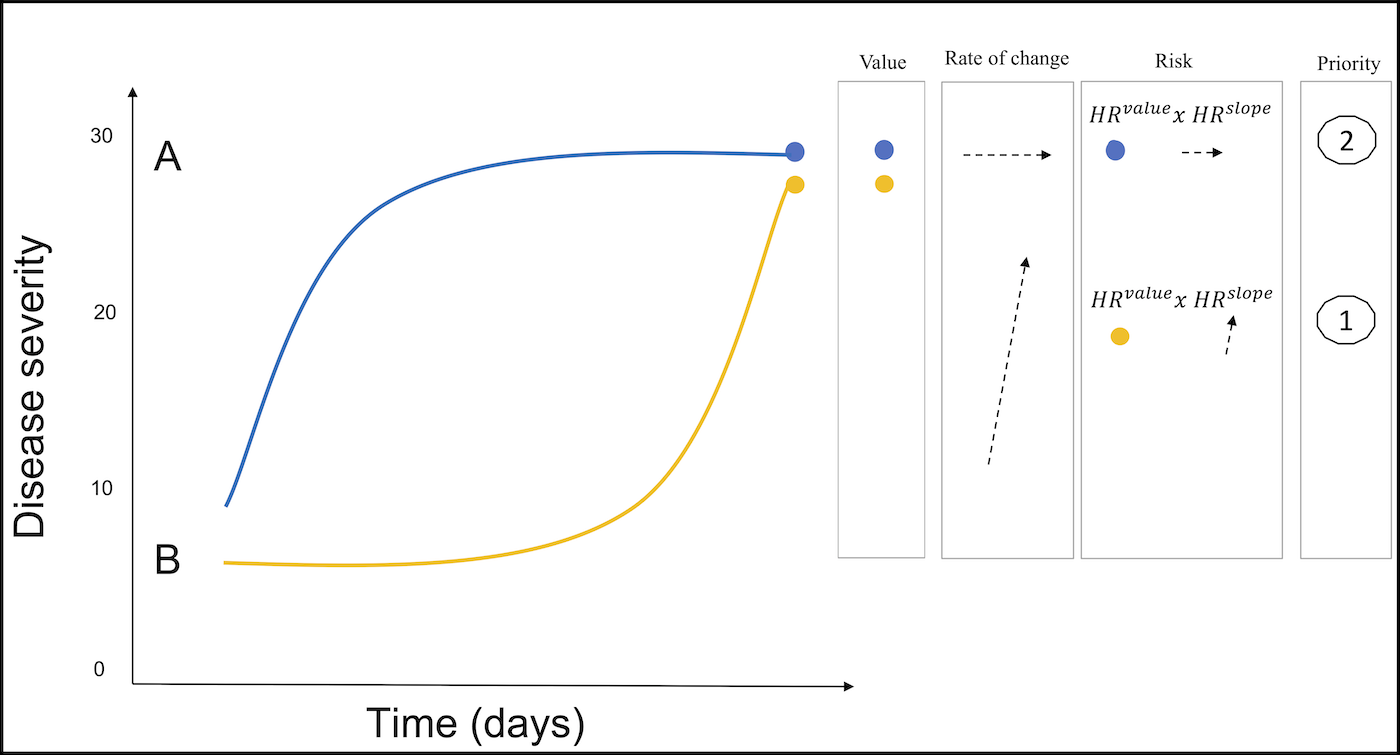
\includegraphics[width=1\linewidth]{figures/jm/figure 1} \caption{Two hypothetical patient trajectories on the LT waiting list are shown. Patient A initially increases and then stabilizes in disease severity. B is initially stable and later deteriorates. Under the current MELD(-Na) allocation, patient A would be prioritized over patient B in liver allocation, because the most recent MELD(-Na) is used. However, the JM uses both the past and current disease severity (value) and the rate of change at each moment in time (slope). At any given time, the JM combines the hazard ratio’s for value and slope to calculate the risk of death. Thus, the JM would calculate a higher mortality risk and thus LT priority for patient B, because the disease is increasing fast.}\label{fig:jm-fig1}
\end{figure}

\hypertarget{prediction-performance}{%
\subsection*{Prediction performance}\label{prediction-performance}}
\addcontentsline{toc}{subsection}{Prediction performance}

The JMs ability to predict 90-day mortality was assessed by calculating the area under the receiver operator curve (AUC) and prediction errors (Brier scores). Model performance was assessed at baseline (start of waiting list follow-up) and 3-monthly during follow-up of two years through bootstrap cross validation with 100 repetitions. To clarify, patients were censored if they did not die, but their data up until censoring would still be used when calculating performance. For comparison to currently-used models, MELD(-Na) prediction performance was also calculated at these time points.

\hypertarget{impact-on-the-waiting-list-2}{%
\subsection*{Impact on the waiting list}\label{impact-on-the-waiting-list-2}}
\addcontentsline{toc}{subsection}{Impact on the waiting list}

Next, we estimated the possible impact of using the JMs instead of MELD(-Na) for waiting list prioritization. To do this, data from baseline to 90 days was used. At day 90, patients still on the waiting list were ranked highest-to-lowest based on their predicted 90-day mortality probability. This created a different ranking for the MELD(Na)-JM and MELD(-Na) models. The number of available donor livers in the first 90 days was then assigned to the highest ranking patients. This created a rough estimate who would have been offered LT first.\textsuperscript{16,17} To further explain the possible differences in prioritization, baseline characteristics and the MELD(-Na) developments over time were compared between patients prioritized either by the MELD(Na)-JM or MELD(-Na).

\hypertarget{online-lt-jm-prediction-tool}{%
\subsection*{Online LT-JM prediction tool}\label{online-lt-jm-prediction-tool}}
\addcontentsline{toc}{subsection}{Online LT-JM prediction tool}

Lastly, online prediction tools of the MELD-JM (\url{https://predictionmodels.shinyapps.io/meld-jm/}) and MELDNa-JM (\url{https://predictionmodels.shinyapps.io/MELDNa-JM/}) were created. This allows interested readers to predict survival probabilities based on individual patient data. For the instruction manual, see supplement page 3. All the analyses were done with R v4.0.0 (R Foundation for Statistical Computing, Vienna, Austria).

\hypertarget{results-2}{%
\section*{Results}\label{results-2}}
\addcontentsline{toc}{section}{Results}

\hypertarget{population-characteristics}{%
\subsection*{Population characteristics}\label{population-characteristics}}
\addcontentsline{toc}{subsection}{Population characteristics}

Table \ref{tab:jm-tab1} shows the baseline characteristics for the Eurotransplant and UNOS populations. The 16,283 Eurotransplant LT candidates had a median age of 55 (48-61) at listing. Most (66.3\%) patients were male and the most common liver diseases were (post)alcoholic (39.5\%), cholestatic (11.7\%) and hepatitis-C (10.7\%) induced cirrhosis. At the end of follow-up, 50.2\% were transplanted, 20.9\% deceased, 20.2\% were removed either due to improved clinical condition, priority status or exception points and 8.7\% were censored at the end of study. The 30,533 UNOS patients had a median age of 58 (50-64) years and were mostly (63.3\%) male. Alcohol- (30.5\%) and NASH (20.7\%) related liver cirrhosis were most common. The median MELD at listing was 18 (13-26), which was higher than the MELD 15 (11-21) for the Eurotransplant region. Median MELD-Na at listing was 19 (12-27) points in the UNOS cohort. At the end of follow-up, 52.2\% was transplanted, 13\% had died while waiting or was removed because of worsening clinical condition 31\% was removed due to improved condition, exception point or status 1 approval during follow-up and 3.8\% was censored at the end of study.

\linespread{1}

\begin{table}

\caption{\label{tab:jm-tab1}Baseline characteristics for the Eurotransplant and UNOS regions}
\centering
\resizebox{\linewidth}{!}{
\begin{threeparttable}
\begin{tabular}[t]{lll}
\toprule
Region & Eurotransplant & UNOS\\
\midrule
\cellcolor{gray!6}{study interval} & \cellcolor{gray!6}{2007-2018} & \cellcolor{gray!6}{2016-2019}\\
n & 16283 & 30533\\
\cellcolor{gray!6}{Age (median (IQR))} & \cellcolor{gray!6}{55.0 [48.0, 61.0]} & \cellcolor{gray!6}{58.0 [50.0, 64.0]}\\
Gender male (\%) & 10796 (66.3) & 19334 (63.3)\\
\cellcolor{gray!6}{BMI (median (IQR))} & \cellcolor{gray!6}{25.6 [22.9, 29.2]} & \cellcolor{gray!6}{29.0 [25.0, 33.0]}\\
\addlinespace[0.3em]
\multicolumn{3}{l}{\textbf{Disease (\%)}}\\
\hspace{1em}Cirrhosis, Alcoholic & 6432 (39.5) & 9309 (30.5)\\
\hspace{1em}\cellcolor{gray!6}{Cirrhosis, HCV} & \cellcolor{gray!6}{1742 (10.7)} & \cellcolor{gray!6}{4001 (13.1)}\\
\hspace{1em}Cirrhosis, NASH & NA & 6328 (20.7)\\
\hspace{1em}\cellcolor{gray!6}{Cirrhosis, other causes} & \cellcolor{gray!6}{3794 (23.3)} & \cellcolor{gray!6}{4754 (15.6)}\\
\hspace{1em}Cholestatic disease & 1905 (11.7) & 2422 (7.9)\\
\hspace{1em}\cellcolor{gray!6}{Other} & \cellcolor{gray!6}{2410 (14.8)} & \cellcolor{gray!6}{3725 (12.2)}\\
\addlinespace[0.3em]
\multicolumn{3}{l}{\textbf{Serum measurement at listing (mean (SD))}}\\
\hspace{1em}Creatinine in mg/dL & 1.3 (3.0) & 1.5 (1.4)\\
\hspace{1em}\cellcolor{gray!6}{Bilirubin in mg/dL} & \cellcolor{gray!6}{6.0 (10.6)} & \cellcolor{gray!6}{7.0 (9.4)}\\
\hspace{1em}INR & 1.5 (0.6) & 1.8 (0.9)\\
\hspace{1em}\cellcolor{gray!6}{Sodium in mmol/L} & \cellcolor{gray!6}{NA} & \cellcolor{gray!6}{136 (5.0)}\\
Dialysis dependency (\%) & 937 (5.8) & 3223 (10.6)\\
\cellcolor{gray!6}{MELD at listing (median(IQR))} & \cellcolor{gray!6}{15.0 [11.0, 21.0]} & \cellcolor{gray!6}{18.0 [13.0, 26.0]}\\
MELD-Na at listing (median(IQR)) & NA & 19.0 [12.0, 27.0]\\
\addlinespace[0.3em]
\multicolumn{3}{l}{\textbf{Status at delisting (\%)}}\\
\hspace{1em}\cellcolor{gray!6}{Transplanted} & \cellcolor{gray!6}{8174 (50.2)} & \cellcolor{gray!6}{15928 (52.2)}\\
\hspace{1em}Deceased & 3404 (20.9) & 3974 (13.0)\\
\hspace{1em}\cellcolor{gray!6}{Removed from the waiting list} & \cellcolor{gray!6}{3289 (20.2)} & \cellcolor{gray!6}{9460 (31.0)}\\
\hspace{1em}Censored at study end & 1417 (8.7) & 1171 (3.8)\\
\bottomrule
\end{tabular}
\begin{tablenotes}
\item \textit{Note: } 
\item NA: Eurotransplant has no complete data regarding this item, HCV: hepatitis-C induced, HCC: hepatocellular carcinoma,HU: high urgent status, NSE: (non)standard exception points, MELD: Model of End-stage Liver Disease
\end{tablenotes}
\end{threeparttable}}
\end{table}

\linespread{1.213}

\hypertarget{jm-properties}{%
\subsection*{JM properties}\label{jm-properties}}
\addcontentsline{toc}{subsection}{JM properties}

The JMs calculates hazard ratios at a specific time (\(HR_{t}\)) through the following equations, for MELD-JM: \[{HR}_t=\left({1.29}^{{MELD}_{value}}\right)\ast\left({8.12}^{{MELD}_{slope}}\right)\] and MELDNa-JM: \[{HR}_t=\left({1.24}^{{MELDNa}_{value}}\right)\ast\left({8.02}^{{MELDNa}_{slope}}\right)\] The MELD-JM coefficient for MELD values is 1.29, with 95\% CI (1.28-1.31). The MELD-JM slope coefficient is 8.12 (95\% CI 1.27-50.38). For the MELDNa-JM these are 1.23 (95\% CI 1.24-1.26) and 8.02 (95\% CI 3.65-17.1) respectively. This means that at a given moment in time, a 1-point increase in MELD value will increase mortality risk by a factor 1.29, and a 1-point faster or slower change gives a factor 8.12 difference. These equations, combined with the baseline risks, can be used to calculate specific risks. However, the JM is needed to calculate the MELD(-Na) value and slope at a given time point. To enable easy access to JM predictions, we developed online applications of the MELD-JM (\url{https://predictionmodels.shinyapps.io/meld-jm/}) and MELDNa-JM (\url{https://predictionmodels.shinyapps.io/MELDNa-JM/}). Interested readers can upload repeated MELD(-Na) measurements of individual patients into these applications, to generate personalized predictions. See supplement page 3 for an instruction manual. The performance of these JMs is tested below.

\hypertarget{jm-performance}{%
\subsection*{JM performance}\label{jm-performance}}
\addcontentsline{toc}{subsection}{JM performance}

The JM performance was assessed in the independent validation data at baseline (Figure \ref{fig:jm-fig2} and figure S1) and during follow-up (Table \ref{tab:jm-tab2}: UNOS, table S1: Eurotransplant).

\begin{figure}
\subfloat[90-day mortality ROC plot of the MELDNa-JM and MELD-Na.\label{fig:jm-fig2-1}]{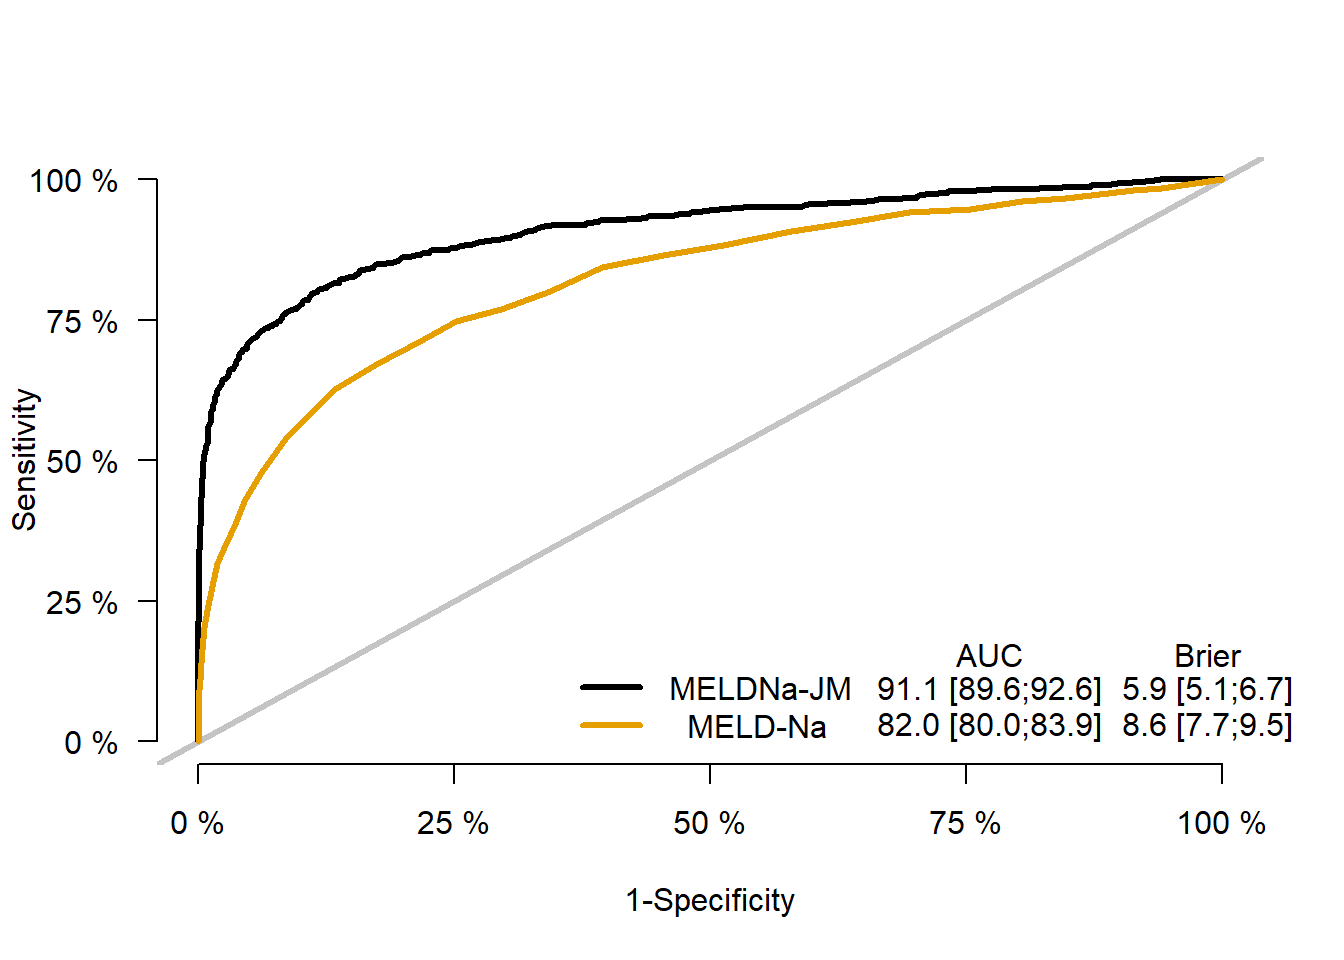
\includegraphics{thesis_files/figure-latex/jm-fig2-1} }\newline\subfloat[Calibration plot of the MELDNa-JM and MELD-Na score. Each dot represents 10 percent of the population. The lines show how well the predicted risks match the observed risks\label{fig:jm-fig2-2}]{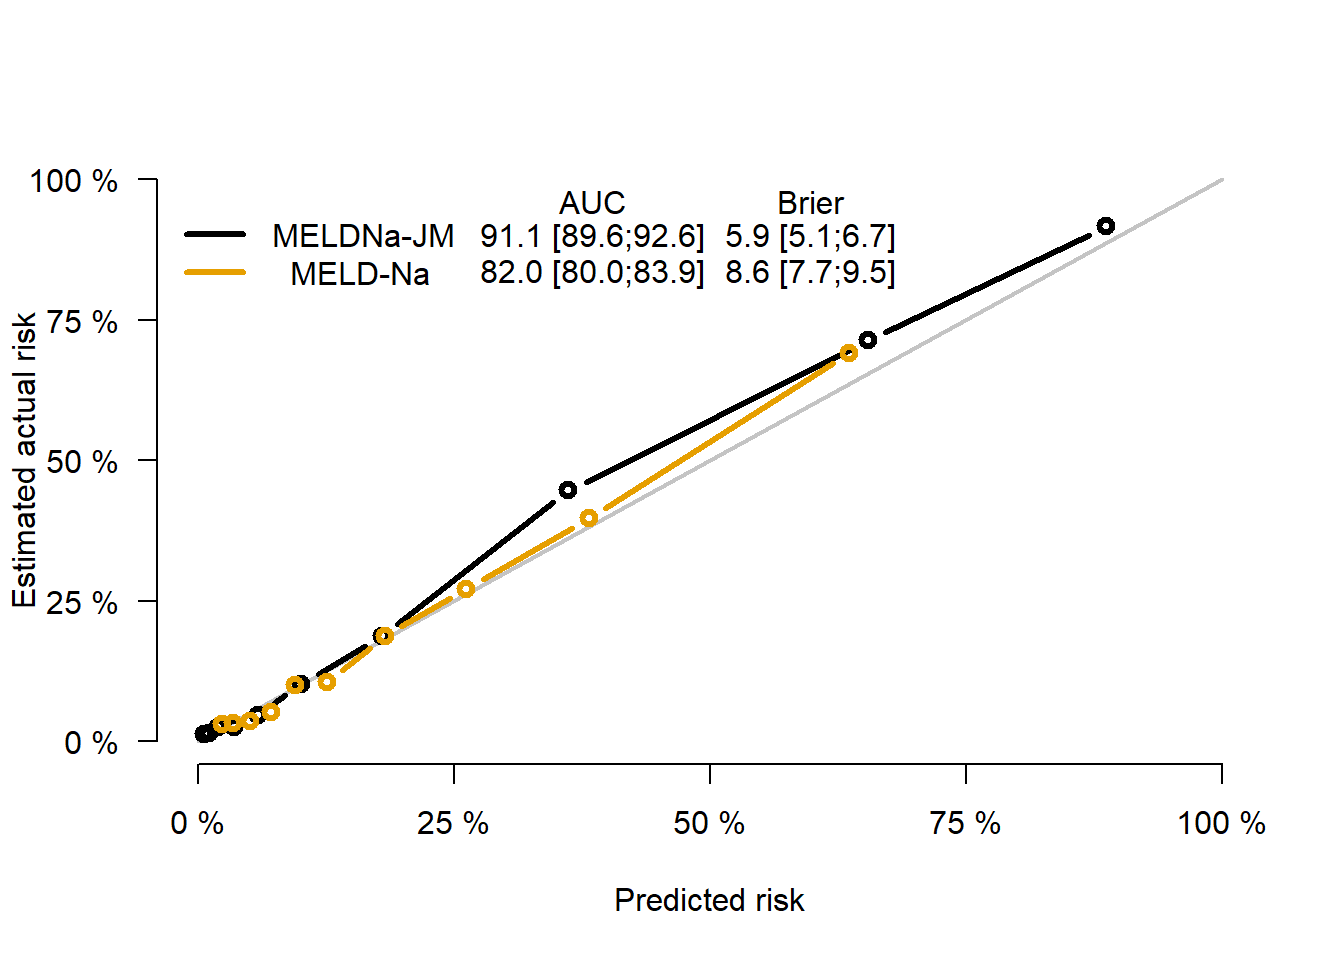
\includegraphics{thesis_files/figure-latex/jm-fig2-2} }\caption{Performance measures for the MELDNa-JM and MELD-Na.}\label{fig:jm-fig2}
\end{figure}

\begin{table}

\caption{\label{tab:jm-tab2}90-day mortality AUCs of the MELDNa-JM versus the MELD-Na, at baseline and during waiting list follow-up in the validation cohort.}
\centering
\resizebox{\linewidth}{!}{
\begin{threeparttable}
\begin{tabular}[t]{rrrrrrrl}
\toprule
\multicolumn{1}{c}{ } & \multicolumn{3}{c}{MELDNa-JM} & \multicolumn{3}{c}{MELD-Na} & \multicolumn{1}{c}{ } \\
\cmidrule(l{3pt}r{3pt}){2-4} \cmidrule(l{3pt}r{3pt}){5-7}
Time (months) & AUC & low95 & upp95 & AUC & low95 & upp95 & p\\
\midrule
\cellcolor{gray!6}{0} & \cellcolor{gray!6}{0.91} & \cellcolor{gray!6}{0.89} & \cellcolor{gray!6}{0.93} & \cellcolor{gray!6}{0.84} & \cellcolor{gray!6}{0.81} & \cellcolor{gray!6}{0.87} & \cellcolor{gray!6}{<0.001}\\
3 & 0.79 & 0.75 & 0.82 & 0.67 & 0.62 & 0.73 & <0.001\\
\cellcolor{gray!6}{6} & \cellcolor{gray!6}{0.80} & \cellcolor{gray!6}{0.76} & \cellcolor{gray!6}{0.84} & \cellcolor{gray!6}{0.69} & \cellcolor{gray!6}{0.61} & \cellcolor{gray!6}{0.75} & \cellcolor{gray!6}{<0.001}\\
9 & 0.81 & 0.75 & 0.86 & 0.75 & 0.69 & 0.81 & <0.001\\
\cellcolor{gray!6}{12} & \cellcolor{gray!6}{0.74} & \cellcolor{gray!6}{0.66} & \cellcolor{gray!6}{0.81} & \cellcolor{gray!6}{0.69} & \cellcolor{gray!6}{0.58} & \cellcolor{gray!6}{0.79} & \cellcolor{gray!6}{NS}\\
15 & 0.76 & 0.67 & 0.84 & 0.70 & 0.54 & 0.83 & <0.001\\
\cellcolor{gray!6}{18} & \cellcolor{gray!6}{0.78} & \cellcolor{gray!6}{0.69} & \cellcolor{gray!6}{0.86} & \cellcolor{gray!6}{0.76} & \cellcolor{gray!6}{0.62} & \cellcolor{gray!6}{0.87} & \cellcolor{gray!6}{NS}\\
21 & 0.88 & 0.78 & 0.97 & 0.83 & 0.62 & 0.96 & NS\\
\cellcolor{gray!6}{24} & \cellcolor{gray!6}{0.72} & \cellcolor{gray!6}{0.60} & \cellcolor{gray!6}{0.85} & \cellcolor{gray!6}{0.68} & \cellcolor{gray!6}{0.42} & \cellcolor{gray!6}{0.86} & \cellcolor{gray!6}{NS}\\
\bottomrule
\end{tabular}
\begin{tablenotes}
\item \textit{Note: } 
\item AUC: area under receiver operator curve, JM: joint model, MELD-Na: model for end-stage liver disease sodium score
\end{tablenotes}
\end{threeparttable}}
\end{table}

At baseline, MELDNa-JM AUC was 0.91 (0.89-0.93) and MELD-Na AUC was 0.84 (0.81-0.87). In Eurotransplant, MELD-JM AUC was 0.94 (95\% CI 0.92-0.95) compared to 0.87 (0.85-0.89) for MELD (figures S1 and S2). For both the MELD(Na)-JM and MELD(-Na), prediction performance was best in the first months of follow-up. The MELD(Na)-JMs AUCs were significantly (p\textless0.001) better than the MELD(-Na) for the first 12 months of follow-up. During this period, the majority of transplantations was done, i.e.~94\% (UNOS) and 84\% (Eurotransplant). After 12 months, JMs AUCs were still notably but not significantly better than MELD(-Na). Over time, MELD(-Na) might be less representative of disease severity in LT candidates, which could explain the decrease in AUC over time for both models. MELD(Na)-JM prediction errors were always significantly lower than the MELD(-Na) (figure 2B, figure S2, tables S1 and S2). In other words, the JMs predictions were more accurate and thus better resembled the observed risks in the population. Subset analysis of prior (2007-2012) versus recent (2013-2018) years showed slightly better performance in the 2007-2012 cohort (table S4). Excluding HCV patients as sensitivity analysis increased AUCs (table S5). MELDNa-JM performed better in males (Figure S5), possibly because MELD-Na tends to underestimate female disease severity through lower creatinine levels.\textsuperscript{18} Performance was comparable for most diseases and worst in HCV disease (Figure S6). The implications for LT candidates might be limited, as the number of listed HCV patients is decreasing.\textsuperscript{19} Performance for non-black candidates was slightly better than for black candidates (Figure S7).

\hypertarget{jm-impact-on-the-waiting-list}{%
\subsection*{JM impact on the waiting list}\label{jm-impact-on-the-waiting-list}}
\addcontentsline{toc}{subsection}{JM impact on the waiting list}

The possible differences in MELDNa-JM and MELD-Na prioritization were assessed. Table \ref{tab:jm-tab3} shows the baseline characteristics of patients that would have been prioritized both by MELDNa-JM and MELD-Na, by one of the models or by neither (table S6: MELD and MELD-JM comparison).

\begin{landscape}\begin{table}

\caption{\label{tab:jm-tab3}Characteristics of prioritized recipients.}
\centering
\resizebox{\linewidth}{!}{
\begin{tabular}[t]{llllll}
\toprule
Characteristics & Both & MELDNa-JM 
prioritized & MELD-Na 
prioritized & Not prioritized & p\\
\midrule
\cellcolor{gray!6}{n} & \cellcolor{gray!6}{3196} & \cellcolor{gray!6}{611} & \cellcolor{gray!6}{611} & \cellcolor{gray!6}{5658} & \cellcolor{gray!6}{}\\
Age (median [IQR]) & 55.0 [47.0, 62.0] & 56.0 [48.0, 63.0] & 58.0 [51.0, 63.0] & 59.0 [53.0, 64.0] & <0.001\\
\cellcolor{gray!6}{Female sex (\%)} & \cellcolor{gray!6}{1209 (37.8)} & \cellcolor{gray!6}{284 (46.5)} & \cellcolor{gray!6}{216 (35.4)} & \cellcolor{gray!6}{1978 (35.0)} & \cellcolor{gray!6}{<0.001}\\
BMI (mean (SD)) & 29.9 (6.6) & 28.5 (6.6) & 28.6 (5.8) & 29.1 (5.9) & <0.001\\
\cellcolor{gray!6}{Death within 90 days (\%)} & \cellcolor{gray!6}{498 (15.6)} & \cellcolor{gray!6}{94 (15.4)} & \cellcolor{gray!6}{26 (4.3)} & \cellcolor{gray!6}{135 (2.4)} & \cellcolor{gray!6}{<0.001}\\
\addlinespace[0.3em]
\multicolumn{6}{l}{\textbf{Disease (\%)}}\\
\hspace{1em}Cirrhosis HCV & 235 (7.4) & 39 (6.4) & 87 (14.2) & 973 (17.2) & \\
\hspace{1em}\cellcolor{gray!6}{NASH} & \cellcolor{gray!6}{597 (18.7)} & \cellcolor{gray!6}{140 (22.9)} & \cellcolor{gray!6}{138 (22.6)} & \cellcolor{gray!6}{1204 (21.3)} & \cellcolor{gray!6}{}\\
\hspace{1em}Cirrhosis Alcoholic & 1413 (44.2) & 209 (34.2) & 230 (37.6) & 1245 (22.0) & \\
\hspace{1em}\cellcolor{gray!6}{Cirrhosis Other} & \cellcolor{gray!6}{575 (18.0)} & \cellcolor{gray!6}{108 (17.7)} & \cellcolor{gray!6}{83 (13.6)} & \cellcolor{gray!6}{761 (13.4)} & \cellcolor{gray!6}{}\\
\hspace{1em}Cholestatic disease & 185 (5.8) & 68 (11.1) & 33 (5.4) & 533 (9.4) & \\
\hspace{1em}\cellcolor{gray!6}{Metabolic disease} & \cellcolor{gray!6}{73 (2.3)} & \cellcolor{gray!6}{16 (2.6)} & \cellcolor{gray!6}{13 (2.1)} & \cellcolor{gray!6}{107 (1.9)} & \cellcolor{gray!6}{}\\
\hspace{1em}Malignant/benign tumor & 52 (1.6) & 12 (2.0) & 22 (3.6) & 705 (12.5) & \\
\hspace{1em}\cellcolor{gray!6}{Other} & \cellcolor{gray!6}{66 (2.1)} & \cellcolor{gray!6}{19 (3.1)} & \cellcolor{gray!6}{5 (0.8)} & \cellcolor{gray!6}{130 (2.3)} & \cellcolor{gray!6}{}\\
MELD (median [IQR]) & 30.0 [26.0, 37.0] & 21.0 [18.0, 24.0] & 22.0 [19.0, 24.0] & 14.0 [10.0, 17.0] & <0.001\\
\cellcolor{gray!6}{MELD-Na (median [IQR])} & \cellcolor{gray!6}{31.0 [27.0, 35.0]} & \cellcolor{gray!6}{21.0 [19.0, 22.0]} & \cellcolor{gray!6}{25.0 [24.0, 27.0]} & \cellcolor{gray!6}{13.0 [9.0, 17.0]} & \cellcolor{gray!6}{<0.001}\\
\bottomrule
\end{tabular}}
\end{table}
\end{landscape}

Compared to MELD-Na, the MELDNa-JM prioritized slightly younger (56 vs 58 years) and female (46.5\% vs 35.4\%) patients, who less often had hepatitis-C-induced liver cirrhosis. Most importantly, MELDNa-JM-prioritized patients had a 3.6 times higher 90-day mortality rate, i.e.~15.4\% versus 4.3\%. For the Eurotransplant region, MELD-JM prioritized patients with 5.0 times higher 90-day mortality compared to MELD, i.e.~23.2\% versus 4.6\% (table S6). A possible cause of this difference in mortality is illustrated in Figure \ref{fig:jm-fig3}.

\begin{figure}
\centering
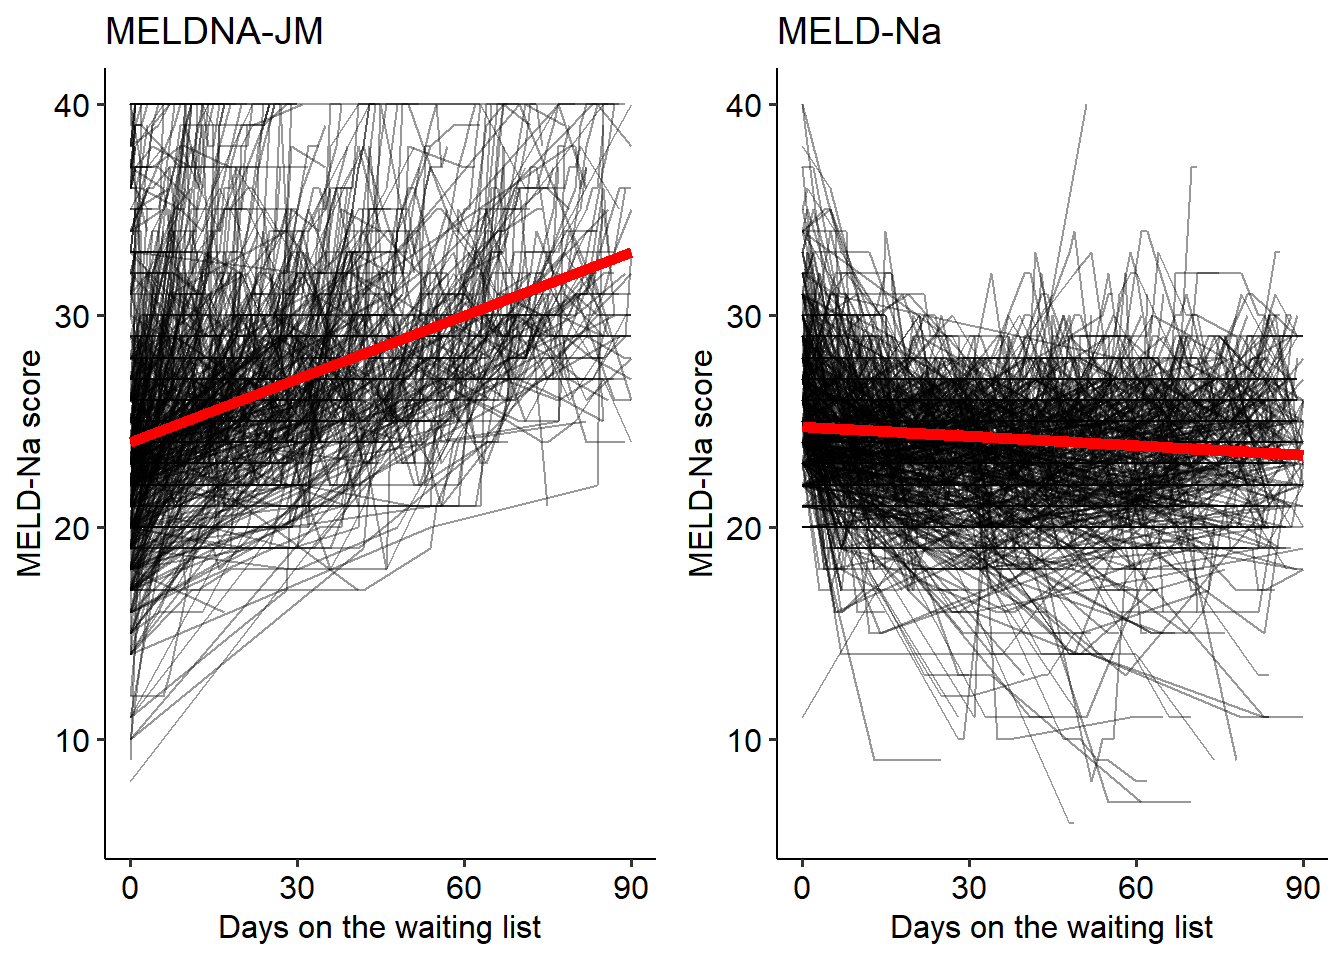
\includegraphics{thesis_files/figure-latex/jm-fig3-1.pdf}
\caption{\label{fig:jm-fig3}The MELDNa- JM and MELD- Na would prioritize different patients for liver transplantation. For these patients, we plotted the individual (black lines) and average (red line) MELD-Na score development during 90 days. Although the MELD-Na-prioritized patients had a higher initial MELD-Na score (value), their average scores remained stable (slope). In contrast, the JM-prioritized patients had lower MELD-Na (value) scores but with faster increasing disease severity (slope). Interestingly, the JM- prioritized patients had a five times higher 90- day mortality rate. Indicating that JM prioritization could possibly be more just.}
\end{figure}

The JM prioritized patients with lower median MELD-Na scores, see Table \ref{tab:jm-tab3}, but these patients had increasing disease severity at the time of liver graft allocation. This illustrates how not only the MELD-Na value, but also the rate of change is considered when estimating survival (figure S3 for Eurotransplant plots). The MELDNa-JM could therefore have prioritized patients with a higher waiting list mortality, possibly not captured by MELD-Na.

\hypertarget{online-prediction-tools}{%
\subsection*{Online prediction tools}\label{online-prediction-tools}}
\addcontentsline{toc}{subsection}{Online prediction tools}

To access MELD-JM or MELDNa-JM predictions for the individual patient, please visit respectively \url{https://predictionmodels.shinyapps.io/meld-jm/} or \url{https://predictionmodels.shinyapps.io/MELDNa-JM/}. See page 3 of the supplement for instructions. For clinical JM implementation in individual patients, repeated measurements of MELD(-Na) can be loaded into the online app. This essentially is the same data as uploaded to organ procurement organizations. The JM app then calculates prognosis based on these measurements and lets the user choose the moment in time and prediction horizon, e.g.~assess 90-day survival probabilities after five months of waiting. These individual predictions can improve clinical decision making.

\hypertarget{discussion-2}{%
\section*{Discussion}\label{discussion-2}}
\addcontentsline{toc}{section}{Discussion}

This retrospective cohort analysis aimed to improve LT candidate survival prediction by using longitudinal data. Therefore, we developed and validated the MELD-JM and MELDNa-JM for waiting list mortality prediction in the Eurotransplant and UNOS regions. We report several important findings. First, the JM-calculated MELD(-Na) values and their time-dependent rate of change are significantly associated with LT candidate waiting list mortality. Second, using time-dependent value and slope, the JMs significantly outperformed both MELD and MELD-Na when predicting mortality. Third, the JMs would have prioritized patients with three to five times higher mortality on the waiting list, who would not have been prioritized under MELD(-Na).

\hypertarget{longitudinal-analysis-1}{%
\subsection*{Longitudinal analysis}\label{longitudinal-analysis-1}}
\addcontentsline{toc}{subsection}{Longitudinal analysis}

The progression of liver disease changes within and between patients over time. The current models that determine transplantation priority for patients with end-stage liver disease, i.e.~the MELD(-Na), ignore previous disease development. However, for the clinician it is evident that the history of disease is important when estimating prognosis. Therefore, JMs were used to combine longitudinal and survival analysis.\textsuperscript{8} The resulting MELD(Na)-JM estimate both the value and slope - i.e.~current disease severity and the current rate of change- at each new measurement in time to predict survival, while also considering all previous measurements, see Figure \ref{fig:jm-fig1}. The resulting disease developments are a continuous and flexible trajectory over time, whereas e.g.~time-dependent Cox (TDC) models carry the last measured value on forward.\textsuperscript{20} This can fail to adequately model changing disease severity (figure S4) and can lead to underestimation of mortality in severely-ill LT candidates.\textsuperscript{11} The idea of using MELD(-Na) rate of change for survival prediction is not new. Previously, the MELD spike and delta-MELD have been proposed.\textsuperscript{6,21} The MELD spike indicates a 30\% or higher difference between current MELD and the MELD score measured 7 days ago. It is a binary parameter based on cut-offs (30\% and 7 days). However, through joint-modelling, we achieved a continuous representation of disease based on all data (not only assessing 30\% differences or the past 7 days). MELD spike was intended as tiebreaker between patients with the same MELD scores. The JMs could however prioritize patients even if their MELD-Na values are lower, as long as the product of the value and slope is higher, see Figure \ref{fig:jm-fig1} and \ref{fig:jm-fig3}. The delta-MELD is the difference between lowest MELD in previous 30 days and current MELD. It averages the slope over a varying number of previous days or measurements (depending on the date of lowest MELD). In our view, this makes it an imprecise approximation of current rate of change. Still, it is often considered as predictor in LT analysis.\textsuperscript{22--26} However, Bambha et al.~already showed that the effect of delta-MELD depends on the frequency of measurements.\textsuperscript{27} In contrast, the estimated slope of the MELD(Na)-JM is updated with each new measurement and is not altered by the frequency of measurements.

\hypertarget{prediction-performance-1}{%
\subsection*{Prediction performance}\label{prediction-performance-1}}
\addcontentsline{toc}{subsection}{Prediction performance}

The MELD(Na)-JM prediction performance was significantly better than MELD(-Na). The predictions also more accurately resembled the actual survival rates on the waiting list. Models on which treatment decisions are based should ascertain excellent accuracy.\textsuperscript{28} Using additional predictors in JMs, such as age and sex, slightly improved AUCs after 12 months (table S7). However, this was a small improvement, while using these predictors adds to complexity and might be considered unethical. Therefore, MELD(-Na)-only JMs were primarily constructed. Others have also studied possible improvements to MELD(-Na). Recently, a machine-learning MELD-Na alternative was constructed by Bertsimas et al., i.e.~the optimized prediction of mortality (OPOM) model.\textsuperscript{29} Although OPOM outperformed MELD-Na, it also considered more (n=25 or 28) variables. Moreover, OPOM is based on classification analysis, i.e.~is the patient alive after 90 days yes/no, instead of survival analysis, i.e.~how much time passed until death or censoring. Other machine-learning techniques, like random survival forests and neural networks, do not seem to outperform Cox models, even in high-dimensional data.\textsuperscript{30} Previous work did show that JMs outperform time-dependent Cox (TDC) models,\textsuperscript{12--14} which is interesting considering the frequent use of TDC analysis for LT candidates.\textsuperscript{6,7,24,27,31--33} We believe that the TDC last measurement carried-on-forward can give a suboptimal representation of disease (supplement figure 4). With changing disease severity, the TDC model either underestimates or overestimates disease severity. This is especially the case if few measurements are available or data is missing, which often occurs in LT candidate data.

\hypertarget{impact-on-the-waiting-list-3}{%
\subsection*{Impact on the waiting list}\label{impact-on-the-waiting-list-3}}
\addcontentsline{toc}{subsection}{Impact on the waiting list}

We investigated the prioritization differences between the MELDNa-JM and MELD-Na, to give clinical meaning to the found statistical improvements. Considering the rate of change in disease severity helped to identify patients with worse prognosis, which illustrates the concepts shown in Figure \ref{fig:jm-fig1}. To optimize the sickest-first allocation and transplantation benefit, it could therefore be interesting to use the JM-approximated course of disease for LT evaluation. Physicians can use the MELD(Na)-JM as online tool (see above) to predict outcome based on individual patient data. Also, on a center or waiting list population level, JMs can be applied to predict survival of each eligible patient every time a donor liver graft is offered. These predictions can be used alongside or eventually perhaps instead of MELD(-Na), because JM performance is good compared to MELD-Na and the same data is used. This is practical, because no changes would have to be made in the centers' routine of collecting and uploading data.

\hypertarget{limitations-2}{%
\subsection*{Limitations}\label{limitations-2}}
\addcontentsline{toc}{subsection}{Limitations}

A limitation is that data could be missing dependent on unobserved values. Statistical methods, like the JM and Cox model, assume missing at random (MAR) data. For the waiting list, this means that MELD(-Na) missingness should not depend on unobserved values, but it may depend on observed values. Because unobserved values cannot be observed, MAR cannot be proven in this study or any other Eurotransplant/UNOS registry analysis. We did however assess the relation between MELD(-Na) value and reporting frequency (supplement ``missingness analysis''). Involuntary updates of low MELD(-Na) scores were done in only a small part of the data. Also, despite the fact that the most recent score was lower than the previous one, centers still reported these values and often well in time. The average time between measurements that were previously higher or lower did not differ substantially. Dependent missingness in low MELD(-Na) scores could lead to overestimation of waiting list mortality. A solution to alleviate possible bias could be to increase the mandatory update frequency of MELD(-Na) scores. Another limitation is that patients with exception points were excluded, because longitudinal modelling of arbitrarily assigned MELD points does not reflect disease severity. However, JMs could be used to model repeated AFP measurements, tumor characteristics and response to therapy. Also, the difference in waiting list prioritization between the MELD(-Na) and MELD(Na)-JM is a rough estimate, which depends on the chosen interval, i.e.~for a shorter follow-up, presumably prioritization of the two indices would be more similar and vice versa. Furthermore, we did not study postoperative survival if the MELD(Na)-JM would have been used for allocation. This is because the JMs were not used to drive allocation. We therefore only could have assessed postoperative survival after MELD(-Na) allocation and would not know how the JMs would have changed that. These questions concern counterfactual outcomes in causal inference, e.g.~what would have happened to patients had they not been transplanted.\textsuperscript{34} The best way to evaluate a new allocation system is to bring it in practice and measure the difference. Evaluating a new allocation system through simulation is probably the next best option. These extensive simulations were beyond the scope of this study. One should be aware, however, that assessment through simulation is based on intrinsically unverifiable assumptions, namely that with changing the allocation priorities nothing else in the system will change. Lastly, JMs are statistically complex and can give biased results if mis-specified. Therefore, construction should be done with care. To aid clinicians, we made online versions of our models freely available.

\hypertarget{conclusion-2}{%
\section*{Conclusion}\label{conclusion-2}}
\addcontentsline{toc}{section}{Conclusion}

This study developed and validated the MELD-JM and MELDNa-JM prediction models for respectively the Eurotransplant and UNOS regions. The MELD(Na)-JM significantly outperformed current models that drive liver allocation. Thus, patient survival can be dynamically predicted based on past and current disease. These predictions could more accurately direct treatment to those most in need.

\newpage
\linespread{1}
\small

\hypertarget{references-3}{%
\section*{References}\label{references-3}}
\addcontentsline{toc}{section}{References}

\begin{enumerate}
\def\labelenumi{\arabic{enumi}.}
\tightlist
\item
  Eurotransplant. Annual Report 2017.; 2018. www.eurotransplant.org.
\item
  Tschuor C, Ferrarese A, Kuemmerli C, et al.~Allocation of liver grafts worldwide -- Is there a best system? J Hepatol. 2019;71(4):707-718. \url{doi:10.1016/j.jhep.2019.05.025}
\item
  Malinchoc M, Kamath PS, Gordon FD, Peine CJ, Rank J, Ter Borg PCJ. A model to predict poor survival in patients undergoing transjugular intrahepatic portosystemic shunts. Hepatology. 2000;31(4):864-871. \url{doi:10.1053/he.2000.5852}
\item
  Wiesner R, Edwards E, Freeman R, et al.~Model for end-stage liver disease (MELD) and allocation of donor livers. Gastroenterology. 2003;124(1):91-96. \url{doi:10.1053/gast.2003.50016}
\item
  Kim WR, Biggins SW, Kremers WK, et al.~Hyponatremia and Mortality among Patients on the Liver-Transplant Waiting List. N Engl J Med. 2008;359(10):1018-1026. \url{doi:10.1007/s11250-017-1262-3}
\item
  Merion RM, Wolfe RA, Dykstra DM, Leichtman AB, Gillespie B, Held PJ. Longitudinal assessment of mortality risk among candidates for liver transplantation. Liver Transplant. 2003;9(1):12-18. \url{doi:10.1053/jlts.2003.50009}
\item
  Sharma P, Schaubel DE, Sima CS, Merion RM, Lok ASF. Re-weighting the Model for End-Stage Liver Disease Score Components. Gastroenterology. 2008;135(5):1575-1581. \url{doi:10.1053/j.gastro.2008.08.004}
\item
  Rizopoulos R. Joint Models for Longitudinal and Time-to-Event Data: With Applications in R. 1st ed.~Chapman and Hall/CRC; 2012.
\item
  Papageorgiou G, Mauff K, Tomer A, Rizopoulos D. An Overview of Joint Modeling of Time-to-Event and Longitudinal Outcomes. Annu Rev Stat Its Appl. 2019;6(1):223-240. \url{doi:10.1146/annurev-statistics-030718-105048}
\item
  Goudsmit BFJ, Tushuizen ME, Putter H, Braat AE, van Hoek B. The role of the model for end-stage liver disease-sodium score and joint models for 90-day mortality prediction in patients with acute-on-chronic liver failure. J Hepatol. 2021;74(2):475-476. \url{doi:10.1016/j.jhep.2020.08.032}
\item
  Hernaez R, Liu Y, Kramer JR, Rana A, El-serag HB, Kanwal F. Model for end-stage liver disease-sodium underestimates 90-day mortality risk in patients with acute-on-chronic liver failuare. J Hepatol. 2020. \url{doi:10.1016/j.jhep.2020.06.005}
\item
  Arisido MW, Antolini L, Bernasconi DP, Valsecchi MG, Rebora P. Joint model robustness compared with the time-varying covariate Cox model to evaluate the association between a longitudinal marker and a time-to-event endpoint. BMC Med Res Methodol. 2019;19(1):1-13. \url{doi:10.1186/s12874-019-0873-y}
\item
  Rizopoulos D, Takkenberg JJM. Tools \& techniques - Statistics: Dealing with time-varying covariates in survival analysis - joint models versus Cox models. EuroIntervention. 2014;10(2):285-288. \url{doi:10.4244/EIJV10I2A47}
\item
  Campbell KR, Juarez-Colunga E, Grunwald GK, Cooper J, Davis S, Gralla J. Comparison of a time-varying covariate model and a joint model of time-to-event outcomes in the presence of measurement error and interval censoring: Application to kidney transplantation. BMC Med Res Methodol. 2019;19(1):1-12. \url{doi:10.1186/s12874-019-0773-1}
\item
  Rizopoulos D. The R package jmbayes for fitting joint models for longitudinal and time-to-event data using MCMC. J Stat Softw. 2016;72(7). \url{doi:10.18637/jss.v072.i07}
\item
  Goudsmit BFJ, Putter H, Tushuizen ME, et al.~Refitting the model for end-stage liver disease for the Eurotransplant region. Hepatology. 2020;in press.
\item
  Leise MD, Kim WR, Kremers WK, Larson JJ, Benson JT, Therneau TM. A revised model for end-stage liver disease optimizes prediction of mortality among patients awaiting liver transplantation. Gastroenterology. 2011;140(7):1952-1960. \url{doi:10.1053/j.gastro.2011.02.017}
\item
  Myers RP, Shaheen AAM, Aspinall AI, Quinn RR, Burak KW. Gender, renal function, and outcomes on the liver transplant waiting list: Assessment of revised MELD including estimated glomerular filtration rate. J Hepatol. 2011;54(3):462-470. \url{doi:10.1016/j.jhep.2010.07.015}
\item
  Kwong AJ, Kim WR, Lake JR, et al.~OPTN/SRTR 2019 Annual Data Report: Liver. Am J Transplant. 2021;21(S2):208-315. \url{doi:10.1111/ajt.16494}
\item
  Dekker FW, De Mutsert R, Van Dijk PC, Zoccali C, Jager KJ. Survival analysis: Time-dependent effects and time-varying risk factors. Kidney Int. 2008;74(8):994-997. \url{doi:10.1038/ki.2008.328}
\item
  Massie AB, Luo X, Alejo JL, Poon AK, Cameron AM, Segev DL. Higher Mortality in Registrants With Sudden Model for End-Stage Liver Disease Increase: Disadvantaged by the Current Allocation Policy. Liver Transplant. 2015;21(5):683-689. \url{doi:10.1002/lt}
\item
  Belli LS, Berenguer M, Cortesi PA, et al.~Delisting of liver transplant candidates with chronic hepatitis C after viral eradication: A European study. J Hepatol. 2016;65(3):524-531. \url{doi:10.1016/j.jhep.2016.05.010}
\item
  Cholankeril G, Li AA, Dennis BB, et al.~Pre-Operative Delta-MELD is an Independent Predictor of Higher Mortality following Liver Transplantation. Sci Rep.~2019;9(1):8312. \url{doi:10.1038/s41598-019-44814-y}
\item
  Györi GP, Silberhumer GR, Rahmel A, et al.~Impact of dynamic changes in MELD score on survival after liver transplantation -- a Eurotransplant registry analysis. Liver Int. 2016;36(7):1011-1017. \url{doi:10.1111/liv.13075}
\item
  Schlegel A, Linecker M, Kron P, et al.~Risk Assessment in High- and Low-MELD Liver Transplantation. Am J Transplant. 2017;17(4):1050-1063. \url{doi:10.1111/ajt.14065}
\item
  Northup PG, Berg CL. Preoperative delta-MELD score does not independently predict mortality after liver transplantation. Am J Transplant. 2004;4(10):1643-1649. \url{doi:10.1111/j.1600-6143.2004.00593.x}
\item
  Bambha K, Kim WR, Kremers WK, et al.~Predicting survival among patients listed for liver transplantation: An assessment of serial MELD measurements. Am J Transplant. 2004;4(11):1798-1804. \url{doi:10.1111/j.1600-6143.2004.00550.x}
\item
  Van Calster B, McLernon DJ, Van Smeden M, et al.~Calibration: The Achilles heel of predictive analytics. BMC Med. 2019;17(1):1-7. \url{doi:10.1186/s12916-019-1466-7}
\item
  Bertsimas D, Kung J, Trichakis N, Wang Y, Hirose R, Vagefi PA. Development and validation of an optimized prediction of mortality for candidates awaiting liver transplantation. Am J Transplant. 2019;19(4):1109-1118. \url{doi:10.1111/ajt.15172}
\item
  Kantidakis G, Putter H, Lancia C, Boer JD, Braat A, Fiocco M. Survival prediction models since liver transplantation - comparisons between Cox models and machine learning techniques. BMC Med Res Methodol. 2020;20(277):1-14. \url{doi:10.21203/rs.3.rs-22670/v1}.
\item
  Luo X, Leanza J, Massie AB, et al.~MELD as a metric for survival benefit of liver transplantation. Am J Transplant. 2018;18(5):1231-1237. \url{doi:10.1111/ajt.14660}
\item
  Schaubel DE, Guidinger MK, Biggins SW, et al.~Survival benefit-based deceased-donor liver allocation. Am J Transplant. 2009;9(4 PART 2):970-981. \url{doi:10.1111/j.1600-6143.2009.02571.x}
\item
  Sharma P, Schaubel DE, Gong Q, Guidinger M, Merion RM. End-stage liver disease candidates at the highest model for end-stage liver disease scores have higher wait-list mortality than status-1A candidates. Hepatology. 2012;55(1):192-198. \url{doi:10.1002/hep.24632}
\item
  van Geloven N, Swanson SA, Ramspek CL, et al.~Prediction meets causal inference: the role of treatment in clinical prediction models. Eur J Epidemiol. 2020;35(7):619-630. \url{doi:10.1007/s10654-020-00636-1}
\end{enumerate}

\newpage
\linespread{1.213}
\normalsize
\thispagestyle{plain}

\mbox{}

\pagecolor{black}
\color{white}

\hypertarget{chap-aclfjm}{%
\chapter{Development and validation of a dynamic survival prediction model for patients with acute-on-chronic liver failure}\label{chap-aclfjm}}

\chaptermark{Joint Models for ACLF}

\vspace*{\fill}

\noindent Goudsmit BFJ, Braat AE, Tushuizen ME, et al.~Development and validation of a dynamic survival prediction model for patients with acute-on-chronic liver failure. \emph{JHEP Reports}. 2021; doi: 10.1016/j.jhepr.2021.100369.

\begin{center}\rule{0.5\linewidth}{0.5pt}\end{center}

\newpage

\noindent
\nopagecolor
\color{black}
\small

\textbf{Abstract}

\textbf{Background \& Aims}: Acute-on-Chronic-Liver Failure (ACLF) involves an acute deterioration of liver function in patients with chronic liver disease. ACLF is usually associated with a precipitating event and results in the failure of other organ systems and high short-term mortality. Currently-used prediction models fail to adequately estimate prognosis and need for liver transplantation (LT) in ACLF. This study develops and validates a dynamic prediction model for ACLF patients, that uses both longitudinal and survival data.

\textbf{Methods}: Adult patients on the UNOS waitlist for LT between 11.01.2016-31.12.2019 were included. Repeated model for end-stage liver disease sodium (MELD-Na) measurements were jointly-modeled with Cox survival analysis to develop the ACLF joint model (ACLF-JM). Model validation was done in separate testing data with area under curve (AUC) and prediction errors. An online ACLF-JM tool was created for clinical application.

\textbf{Results}: In total, 30,533 patients were included. ACLF grade 1 to 3 was present in respectively 16.4, 10.4 and 6.2\% of the patients. The ACLF-JM predicted survival significantly (p\textless0.001) better than the MELD-Na, both at baseline and during follow-up. For 28- and 90-day predictions, ACLF-JM AUCs ranged between 0.840-0.871 and 0.833-875, respectively. Compared to MELD-Na, AUCs and prediction errors were improved by 23.1\%-62.0\% and 5\%-37.6\% respectively. Also, the ACLF-JM could have prioritized patients who had four times higher waiting list mortality, possibly not identified by MELD-Na.

\textbf{Conclusion}: The ACLF-JM dynamically predicts outcome based on current and past disease severity. Prediction performance is excellent over time, even in ACLF-3 patients. Therefore, the ACLF-JM could be used as clinical tool in the evaluation of prognosis and treatment in patients with ACLF.

\newpage
\normalsize

\hypertarget{introduction-3}{%
\section*{Introduction}\label{introduction-3}}
\addcontentsline{toc}{section}{Introduction}

Liver transplantation (LT) is a lifesaving treatment for patients with acute-on-chronic-liver failure (ACLF). ACLF is characterized by an acute deterioration of liver function in patients with chronic liver disease, often started by a precipitating event. ACLF results in the failure of one or more organs and is associated with high short-term mortality.\textsuperscript{1--3} The current model that prioritizes patients for LT, the Model for End-stage Liver Disease sodium (MELD-Na) score,\textsuperscript{4,5} underestimates disease severity in ACLF.\textsuperscript{6,7} This is because MELD-Na does not consider temporal development of single or multiorgan failure (involving the 6 major organs/systems---i.e.~liver, kidney, brain, coagulation, circulation, and respiration). This underestimation of predicted waitlist mortality results in lower access to transplantation for ACLF patients.\textsuperscript{7} Sundaram et al.~showed that ACLF death and waiting list removal rate were highest in ACLF-3 patients with MELD-Na \textless25.\textsuperscript{8} Given that 20.9\% of UNOS LT candidates between 2005-2016 had a form of ACLF,\textsuperscript{8} the inequal transplantation access might be substantial.

The MELD-Na uses one moment in time, i.e.~the most recent measurement, to predict outcome.\textsuperscript{4,5} It therefore ignores previous data valuable for survival estimation. However, ACLF is a dynamic disease with a clinical course that can change within days, resulting in very different outcomes.\textsuperscript{9,10} Thus, there is a need for prediction models that estimate ACLF survival based on disease development over time.\textsuperscript{7} The Chronic Liver Failure Consortium Organ Failure score (CLIF-C OFs) and CLIF-C ACLF score were developed for this purpose and showed better performance than the MELD-Na.\textsuperscript{3,6} However, they also assessed only one moment in time. A joint model (JM) is a novel prediction model that simultaneously uses longitudinal and survival data.\textsuperscript{11} It approximates changing disease severity over time and uses this for survival prediction.\textsuperscript{12} JMs have shown superior predictive performance over Cox models.\textsuperscript{12--14} However, they have not been applied to ACLF.

We hypothesized that using disease development over time to dynamically predict prognosis could improve survival prediction in ACLF patients. Much like a clinician, we aimed to use disease severity and its rate of change to predict outcome. We believe this is warranted in ACLF, because of the dynamic nature of ACLF disease and the current underestimation of mortality by MELD-Na.\textsuperscript{9,10,15} Therefore, we constructed and validated a multivariate prediction model for survival prediction in ACLF patients: the ACLF Joint Model (ACLF-JM). We investigated the ACLF-JM 28- and 90-day survival prediction performance in the United Network for Organ Sharing (UNOS) registry and compared its performance to the MELD-Na score. We also investigated whether the ACLF-JM would identify patients in whom MELD-Na underestimates mortality. For easy clinical application, an online ACLF-JM tool was developed for dynamic survival prediction in ACLF patients.

\hypertarget{methods-3}{%
\section*{Methods}\label{methods-3}}
\addcontentsline{toc}{section}{Methods}

The TRIPOD statement was used for the development and validation of this multivariate prediction model.\textsuperscript{16}

\hypertarget{study-population-2}{%
\subsection*{Study population}\label{study-population-2}}
\addcontentsline{toc}{subsection}{Study population}

Data of LT candidates was requested from the UNOS. We included adult (\textgreater=18 years) patients listed for a first LT between January 11\textsuperscript{th}, 2016 (after MELD-Na implementation) and December 31\textsuperscript{st}, 2019. We excluded candidates with acute liver failure (ALF) and hepatocellular carcinoma (HCC) at baseline. Data were used from first active listing until the earliest of patient death, transplantation, removal or censor at December 31\textsuperscript{st}, 2019. Death was defined both as death while listed and removal for being too sick to transplant.\textsuperscript{8} If patients received exception points or a status 1 (i.e.~high urgency status) after first listing, they were censored from that date. MELD-Na data was missing in 0.05\%, therefore complete-case analysis was done. Missing values for the predictors life support dependency (variable CAN\_LIFE\_SUPPORT, 0.00009\% missing) and spontaneous bacterial peritonitis (CAN\_BACTERIA\_PERIT, 0.005\% missing) were set to `no.'

\hypertarget{identification-of-aclf}{%
\subsection*{Identification of ACLF}\label{identification-of-aclf}}
\addcontentsline{toc}{subsection}{Identification of ACLF}

Baseline ACLF was defined according to the to the European Foundation for the Study of Chronic Liver Failure (EF Clif) criteria.\textsuperscript{3} Specifically, liver failure was defined as serum bilirubin \textgreater=12 mg/dL, kidney failure as serum creatinine \textgreater=2.0 mg/dL or renal replacement therapy, cerebral failure as presence of hepatic encephalopathy grade 3-4, coagulation failure as INR \textgreater=2.5. Like other authors that used United Network for Organ Sharing (UNOS) data, we used mechanical ventilation as replacement for respiratory failure, since data on PaO2/FiO2 were not available. Also, life-support dependency was used to designate circulatory failure.\textsuperscript{6,8,10,17}

\hypertarget{development-of-the-aclf-jm}{%
\subsection*{Development of the ACLF-JM}\label{development-of-the-aclf-jm}}
\addcontentsline{toc}{subsection}{Development of the ACLF-JM}

Data were randomly split in a training (67\% of the patients) and a testing (33\%) set, for model development and validation respectively. The ACLF-JM consists of two parts: a longitudinal (mixed-effect) and survival (Cox proportional hazards) model. Mixed-effect models were used because they estimate disease development over time as a continuous trajectory and can model both linear (chronic, stable disease) and non-linear (fast deterioration in ACLF) developments. See figure S4 for an illustration. Thus, repeated measurements of MELD-Na scores were modeled with mixed-effects. Additional predictors were used to correct the longitudinal data. To start, 50 candidate variables were assessed (table S2). We excluded some variables a priori, because they referred to pediatric recipients, exclusion criteria, or donor characteristics. Variable relation to mortality was studied in univariate analysis and then variables were backwards selected for multivariate Cox analysis. The final variables included in the model contributed most significantly besides those used for ACLF scoring through EF CliF criteria (serum bilirubin, creatinine, renal replacement therapy, encephalopathy grade, INR, mechanical ventilation, and life-support dependency). Thus, we additionally corrected for candidate age (years), sex (male/female), life support dependency (yes/no), presence of bacterial peritonitis (yes/no), presence of cirrhosis (alcohol-induced, hepatitis-C virus, non-alcoholic steatohepatitis (NASH) or other cirrhosis) (yes/no) and CLIF-C OF score (No ACLF or ACLF grade 1 to 3) (table S1). Next, a Cox proportional hazards model was constructed for waiting list mortality, using the same predictors as the mixed-effect model. Then, the ACLF-JM was constructed by joint-modelling the longitudinal (mixed-effect) and survival (Cox) model.\textsuperscript{18} A key feature is that the ACLF-JM uses both the estimated MELD-Na value and the rate of change in MELD-Na (the slope of the decrease/increase) over time for survival prediction.

\begin{figure}
\centering
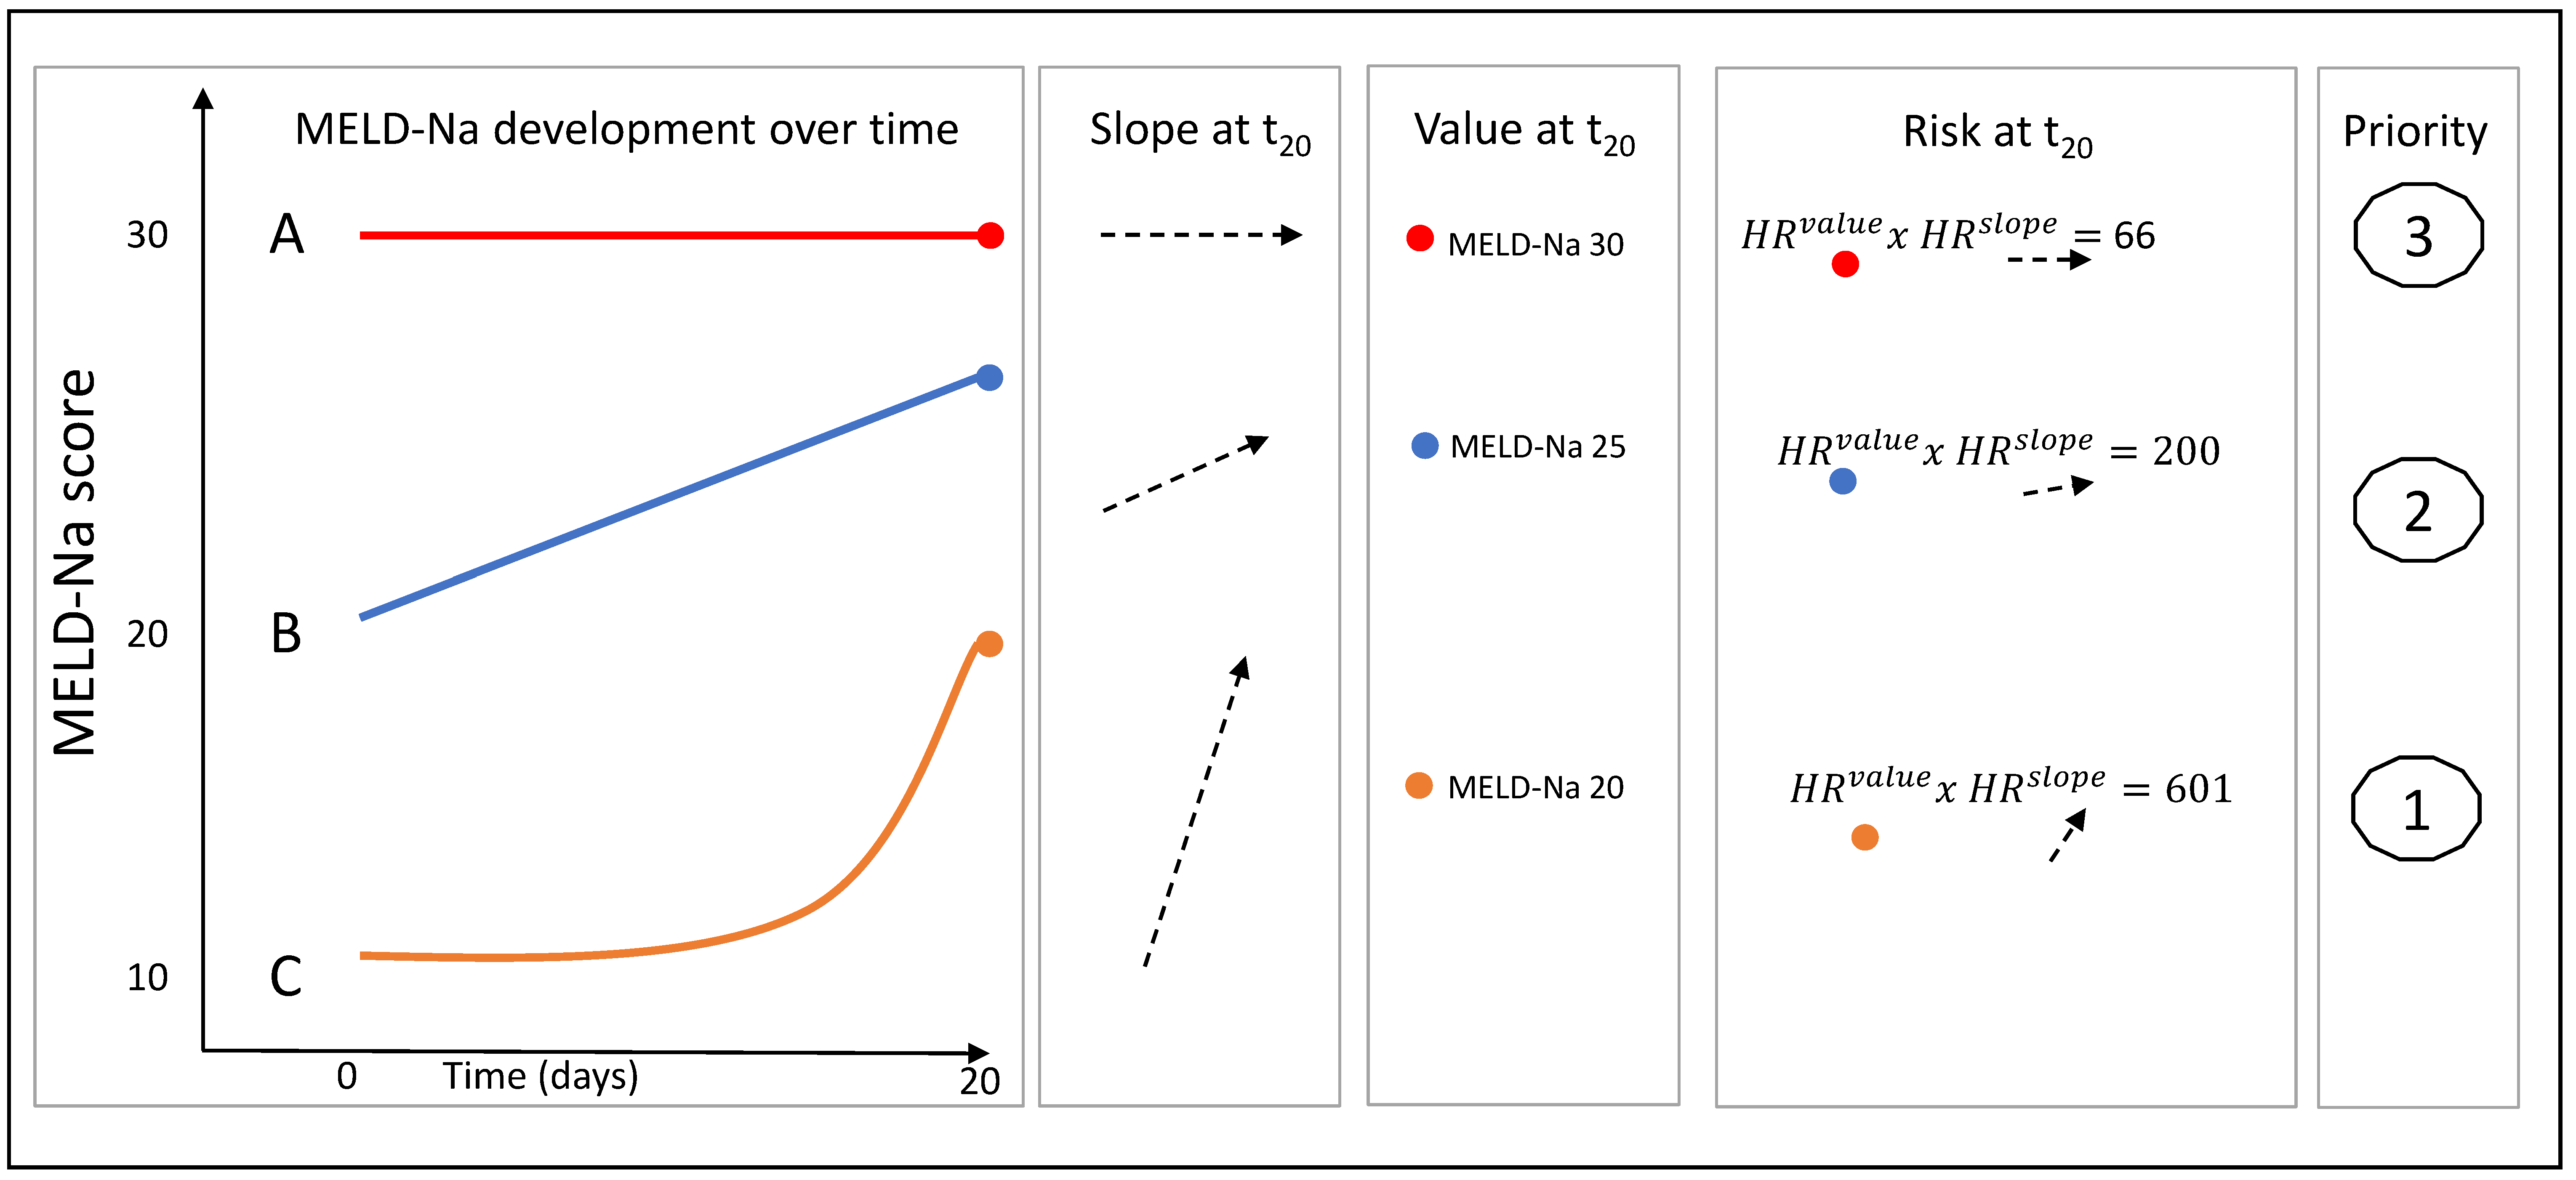
\includegraphics{figures/aclfjm/figure 1.pdf}
\caption{\label{fig:aclf-fig1}Three hypothetical patient MELD-Na trajectories over time, each illustrates differences in value, slope and risk.}
\end{figure}

For clarity, these concepts of value and slope were illustrated in Figure \ref{fig:aclf-fig1}. For three hypothetical patients A, B and C, the 20-day MELD-Na development is shown. After 20 days, patient A has a MELD-Na score of 30 and is thus prioritized by the current allocation system. However, the ACLF-JM uses both the estimated value (measured MELD-Na score) and slope (rate of change) at time=20 for survival prediction. Calculation of the HRs shows that the ACLF-JM gives patient C the greatest risk of death, because of the fast increase in MELD-Na scores (positive slope). See supplement 4 for the precise explanation and calculation.

\hypertarget{validation-of-the-aclf-jm}{%
\subsection*{Validation of the ACLF-JM}\label{validation-of-the-aclf-jm}}
\addcontentsline{toc}{subsection}{Validation of the ACLF-JM}

Next, the prediction performance of the ACLF-JM was compared to the MELD-Na at various points in time in the separate testing data. Specifically, predictions were assessed at baseline and after a follow-up of 48 hours, 7 days and 14 days (similar to the validation study of the CLIF-C OF).\textsuperscript{6} Outcomes were 28-day and 90-day survival. For both the ACLF-JM and MELD-Na Cox model, the area under the receiver-operator-characteristic curve (AUC) and prediction errors were calculated and compared (see supplement 3 for detailed information). These measures and their 95\% confidence intervals (95\%CI) and p-values were calculated using the R package JM and bootstrapping.\textsuperscript{18}

\hypertarget{aclf-jm-impact-on-the-transplantation-waiting-list}{%
\subsection*{ACLF-JM impact on the transplantation waiting list}\label{aclf-jm-impact-on-the-transplantation-waiting-list}}
\addcontentsline{toc}{subsection}{ACLF-JM impact on the transplantation waiting list}

Next, we assessed the possible effect of using the ACLF-JM instead of MELD-Na to estimate mortality and subsequently prioritize patients for LT. This was of interest, because ACLF patients are likely underserved in the current LT allocation.\textsuperscript{15} To assess possible differences in MELD-Na and ACLF-JM waitlist prioritization of patients, we followed patients from baseline until day 28.\textsuperscript{6} Within this period, each time a liver graft was offered, patients were ranked two times from most to least ill based on their estimated survival without transplant. One ranking was made with the ACLF-JM predictions and one based on MELD-Na. Thus, for each model, patients were ranked 2636 times, i.e., the total number of available liver grafts within the first 28 days. After a liver graft offer, the transplanted patient was removed from the waiting list. We assumed that the highest ranked patients were transplanted, which is not necessarily true, and thus that the number of available transplants in the first 28 days represented the threshold of receiving transplantation. We then assessed which patients were prioritized according to what model. After 28 days and 2636 rankings, patients were stratified in four groups: those who are prioritized and possibly transplanted within 28 days according to both scores, those who are prioritized by either the ACLF-JM or MELD-Na score (but not by both) and those who are not prioritized by both. We also assessed the characteristics of the differently-prioritized patients, to see why patients were prioritized differently.

\hypertarget{clinical-application-of-the-aclf-jm}{%
\subsection*{Clinical application of the ACLF-JM}\label{clinical-application-of-the-aclf-jm}}
\addcontentsline{toc}{subsection}{Clinical application of the ACLF-JM}

Lastly, an online version of the ACLF-JM was created (\url{https://predictionmodels.shinyapps.io/aclf-jm/}), which allows clinicians to assess ACLF-JM survival predictions for their individual patient(s). Plots can be created of these dynamic predictions, to show the updating survival estimate for every new available measurement during follow-up. For a instruction manual, see supplement 1 and 2. All statistical analyses were performed using R v4.0.0 (R Foundation for Statistical Computing, Vienna, Austria).

\hypertarget{results-3}{%
\section*{Results}\label{results-3}}
\addcontentsline{toc}{section}{Results}

\hypertarget{study-population-3}{%
\subsection*{Study population}\label{study-population-3}}
\addcontentsline{toc}{subsection}{Study population}

In total, we included 30,533 patients with 249,030 measurements. Table \ref{tab:aclf-tab1} shows the baseline characteristics of the study population. ACLF at baseline was seen in 33.3\% of the patients; 15.9\% had ACLF grade 1, 10.3\% had grade 2 and 7.1\% had grade 3. In these patients, liver (47.2\%) and kidney (63.6\%) failure were the most common. With increasing ACLF grade, median {[}IQR{]} age decreased, ranging from 59 {[}52-64{]} (no ACLF) to 53 {[}43-60{]} years (ACLF-3). Most patients were male (no ACLF: 65.0\%, ACLF: 60\%) and had alcoholic liver disease (no ACLF 25.8\%, ACLF 40\%). For ACLF grades 0 to 3, median {[}IQR{]} MELD-Na scores at listing were 15 {[}10-22{]}, 27 {[}23-31{]}, 33 {[}29-37{]} and 37 {[}31-42{]}. Average time on the waiting list was 150 days for patients without ACLF, 89 for ACLF grade 1, 24 for grade 2 and 10 days for grade 3. Cumulative incidence plots showed significantly higher death and transplantation rates in ACLF patients (figure S1). At the end of follow-up, 10.9\% of the patients without ACLF died. For patients with ACLF grade 1 to 3, death rates were 16.7\%, 14.3\% and 22.4\%, respectively.

\linespread{1}

\begin{landscape}\begin{table}

\caption{\label{tab:aclf-tab1}Baseline characteristics of UNOS liver transplantation candidates between 2016 to 2019 (n=30,533)}
\centering
\resizebox{\linewidth}{!}{
\begin{tabular}[t]{llllllll}
\toprule
Characteristics & No ACLF & ACLF (any grade) & p & ACLF-1 & ACLF-2 & ACLF-3 & p\\
\midrule
\cellcolor{gray!6}{Number of patients (\%)} & \cellcolor{gray!6}{20,384 (66.7)} & \cellcolor{gray!6}{10,149 (33.3)} & \cellcolor{gray!6}{} & \cellcolor{gray!6}{4,843 (15.9)} & \cellcolor{gray!6}{3,147 (10.3)} & \cellcolor{gray!6}{2,159 (7.1)} & \cellcolor{gray!6}{}\\
Age (median [IQR]) & 59 [52, 64] & 55 [47, 62] & <0.001 & 58 [50, 64] & 53 [44, 60] & 53 [43, 60] & <0.001\\
\cellcolor{gray!6}{Male gender} & \cellcolor{gray!6}{13240 (65)} & \cellcolor{gray!6}{6094 (60)} & \cellcolor{gray!6}{<0.001} & \cellcolor{gray!6}{2905 (60.0)} & \cellcolor{gray!6}{1919 (61.0)} & \cellcolor{gray!6}{1270 (58.8)} & \cellcolor{gray!6}{<0.001}\\
BMI (median [IQR]) & 28 [25, 33] & 29 [25, 33] & <0.001 & 28 [24, 33] & 29 [25, 34] & 30 [26, 35] & <0.001\\
\cellcolor{gray!6}{Days waiting (median [IQR])} & \cellcolor{gray!6}{58 [14, 193]} & \cellcolor{gray!6}{12 [4, 40]} & \cellcolor{gray!6}{<0.001} & \cellcolor{gray!6}{27 [9, 93]} & \cellcolor{gray!6}{8 [4, 20]} & \cellcolor{gray!6}{5 [3, 10]} & \cellcolor{gray!6}{<0.001}\\
\addlinespace[0.3em]
\multicolumn{8}{l}{\textbf{Status after waiting}}\\
\hspace{1em}Censored (December 31, 2019) & 986 (4.8) & 185 (1.8) &  & 129 (2.7) & 43 (1.4) & 13 (0.6) & \\
\hspace{1em}\cellcolor{gray!6}{Deceased} & \cellcolor{gray!6}{2229 (10.9)} & \cellcolor{gray!6}{1745 (17.2)} & \cellcolor{gray!6}{} & \cellcolor{gray!6}{810 (16.7)} & \cellcolor{gray!6}{451 (14.3)} & \cellcolor{gray!6}{484 (22.4)} & \cellcolor{gray!6}{}\\
\hspace{1em}Transplanted & 8681 (42.6) & 7247 (71.4) &  & 3187 (65.8) & 2472 (78.6) & 1588 (73.6) & \\
\hspace{1em}\cellcolor{gray!6}{Removed} & \cellcolor{gray!6}{8488 (41.6)} & \cellcolor{gray!6}{972 (9.6)} & \cellcolor{gray!6}{} & \cellcolor{gray!6}{717 (14.8)} & \cellcolor{gray!6}{181 (5.8)} & \cellcolor{gray!6}{74 (3.4)} & \cellcolor{gray!6}{}\\
\addlinespace[0.3em]
\multicolumn{8}{l}{\textbf{Grouped cause of disease (\%)}}\\
\hspace{1em}Cirrhosis HCV & 3084 (15.1) & 917 (9.0) &  & 556 (11.5) & 205 (6.5) & 156 (7.2) & \\
\hspace{1em}\cellcolor{gray!6}{NASH} & \cellcolor{gray!6}{4359 (21.4)} & \cellcolor{gray!6}{1969 (19.4)} & \cellcolor{gray!6}{} & \cellcolor{gray!6}{1184 (24.4)} & \cellcolor{gray!6}{500 (15.9)} & \cellcolor{gray!6}{285 (13.2)} & \cellcolor{gray!6}{}\\
\hspace{1em}Cirrhosis Alcoholic & 5252 (25.8) & 4057 (40.0) &  & 1680 (34.7) & 1431 (45.5) & 946 (43.8) & \\
\hspace{1em}\cellcolor{gray!6}{Cirrhosis Other} & \cellcolor{gray!6}{2976 (14.6)} & \cellcolor{gray!6}{1778 (17.5)} & \cellcolor{gray!6}{} & \cellcolor{gray!6}{682 (14.1)} & \cellcolor{gray!6}{616 (19.6)} & \cellcolor{gray!6}{480 (22.2)} & \cellcolor{gray!6}{}\\
\hspace{1em}Cholestatic disease & 1810 (8.9) & 612 (6.0) &  & 343 (7.1) & 182 (5.8) & 87 (4.0) & \\
\hspace{1em}\cellcolor{gray!6}{Metabolic disease} & \cellcolor{gray!6}{408 (2.0)} & \cellcolor{gray!6}{245 (2.4)} & \cellcolor{gray!6}{} & \cellcolor{gray!6}{112 (2.3)} & \cellcolor{gray!6}{81 (2.6)} & \cellcolor{gray!6}{52 (2.4)} & \cellcolor{gray!6}{}\\
\hspace{1em}Malignant/benign tumor & 2119 (10.4) & 266 (2.6) &  & 194 (4.0) & 42 (1.3) & 30 (1.4) & \\
\hspace{1em}\cellcolor{gray!6}{Other} & \cellcolor{gray!6}{376 (1.8)} & \cellcolor{gray!6}{305 (3.0)} & \cellcolor{gray!6}{} & \cellcolor{gray!6}{92 (1.9)} & \cellcolor{gray!6}{90 (2.9)} & \cellcolor{gray!6}{123 (5.7)} & \cellcolor{gray!6}{}\\
MELD-Na score (median [IQR]) & 15 [10, 20] & 30 [25, 35] & <0.001 & 27 [22, 31] & 33 [29, 37] & 37 [31, 42] & <0.001\\
\cellcolor{gray!6}{Bacterial peritonitis (\%)} & \cellcolor{gray!6}{1560 (7.7)} & \cellcolor{gray!6}{1533 (15.1)} & \cellcolor{gray!6}{<0.001} & \cellcolor{gray!6}{643 (13.3)} & \cellcolor{gray!6}{508 (16.1)} & \cellcolor{gray!6}{329 (17.4)} & \cellcolor{gray!6}{<0.001}\\
\addlinespace[0.3em]
\multicolumn{8}{l}{\textbf{Failure organ/system (\%)}}\\
\hspace{1em}Liver & 540 (2.6) & 4789 (47.2) & <0.001 & 1018 (21.0) & 2007 (63.8) & 1764 (81.7) & <0.001\\
\hspace{1em}\cellcolor{gray!6}{Kidney} & \cellcolor{gray!6}{0 (0.0)} & \cellcolor{gray!6}{6457 (63.6)} & \cellcolor{gray!6}{<0.001} & \cellcolor{gray!6}{2958 (61.1)} & \cellcolor{gray!6}{1717 (54.6)} & \cellcolor{gray!6}{1782 (82.5)} & \cellcolor{gray!6}{<0.001}\\
\hspace{1em}Coagulation & 254 (1.2) & 3699 (36.4) & <0.001 & 667 (13.8) & 1613 (51.3) & 1419 (65.7) & <0.001\\
\hspace{1em}\cellcolor{gray!6}{Cerebral} & \cellcolor{gray!6}{806 (4.0)} & \cellcolor{gray!6}{2095 (20.6)} & \cellcolor{gray!6}{<0.001} & \cellcolor{gray!6}{164 (3.4)} & \cellcolor{gray!6}{697 (22.1)} & \cellcolor{gray!6}{1234 (57.2)} & \cellcolor{gray!6}{<0.001}\\
\hspace{1em}Circulatory & 22 (0.1) & 1193 (11.8) & <0.001 & 36 (0.7) & 221 (7.0) & 936 (43.4) & <0.001\\
\hspace{1em}\cellcolor{gray!6}{Respiratory} & \cellcolor{gray!6}{0 (0.0)} & \cellcolor{gray!6}{662 (6.5)} & \cellcolor{gray!6}{<0.001} & \cellcolor{gray!6}{0 (0.0)} & \cellcolor{gray!6}{39 (1.2)} & \cellcolor{gray!6}{623 (28.9)} & \cellcolor{gray!6}{<0.001}\\
\bottomrule
\end{tabular}}
\end{table}
\end{landscape}

\linespread{1.213}

\hypertarget{model-properties}{%
\subsection*{Model properties}\label{model-properties}}
\addcontentsline{toc}{subsection}{Model properties}

The ACLF-JM is summarized by the equation:
\begin{align*} 
{Hazard\ Ratio\ death}_t={1.15}^{{MELDNa}_{value\ t}}\ast{1.02}^{{MELDNa}_{slope\ t}}\ast{1.38}^{age}\\
\ast{0.75}^{female\ gender}\ast{0.95}^{cirrhosis}\ast\left(if:{1.06}^{ACLF1}\right)\ast\left(if:{1.98}^{ACLF2}\right)\\
\ast\left(if:{5.90}^{ACLF3}\right)\ast{1.18}^{SBP}\ast{1.35}^{life support}
\end{align*}
The ACLF-JM estimates the MELD-Na value and slope at a given timepoint and calculates the HR of death. For each MELD-Na point increase, the risk of 1-year death increases with 15\% (95\% CI 14-16). For every 1-point increase in slope, i.e.~acceleration of disease increase, the mortality risk increases with 2\% (95\% CI 1-2). Of course, in clinical practice, disease severity often changes more rapidly, especially for ACLF patients. A more intuitive illustration of the effect of MELD-Na value and slope is provided in Figure \ref{fig:aclf-fig1}, where three hypothetical patients awaiting LT are shown. The example calculation (details in supplement 4) shows that considering the rate of change (slope) in disease severity adds important information. Considering both MELD-Na value and slope would give priority to patient C (MELD-Na score 20, accelerating disease severity), whereas using the current MELD-Na-based allocation would prioritize patient A (MELD-Na 30, stable disease).

\begin{landscape}\begin{table}

\caption{\label{tab:aclf-tab2}Mortality prediction AUC of the ACLF-JM versus the MELD-Na in patients with and without ACLF, at baseline and during follow-up}
\centering
\resizebox{\linewidth}{!}{
\begin{threeparttable}
\begin{tabular}[t]{lrlrlrlrl}
\toprule
\multicolumn{1}{c}{ } & \multicolumn{4}{c}{ACLF} & \multicolumn{4}{c}{No ACLF} \\
\cmidrule(l{3pt}r{3pt}){2-5} \cmidrule(l{3pt}r{3pt}){6-9}
Time & ACLF-JM & 95\% CI & MELD-Na & 95\% CI & ACLF-JM & 95\% CI & MELD-Na & 95\% CI\\
\midrule
\addlinespace[0.3em]
\multicolumn{9}{l}{\textbf{28-day mortality}}\\
\hspace{1em}\cellcolor{gray!6}{Baseline} & \cellcolor{gray!6}{0.871} & \cellcolor{gray!6}{0.844-0.898} & \cellcolor{gray!6}{0.788} & \cellcolor{gray!6}{0.754-0.822} & \cellcolor{gray!6}{0.774} & \cellcolor{gray!6}{0.717-0.831} & \cellcolor{gray!6}{0.706} & \cellcolor{gray!6}{0.643-0.769}\\
\hspace{1em}48 hours & 0.871 & 0.844-0.898 & 0.786 & 0.752-0.820 & 0.794 & 0.741-0.847 & 0.728 & 0.668-0.788\\
\hspace{1em}\cellcolor{gray!6}{7 days} & \cellcolor{gray!6}{0.862} & \cellcolor{gray!6}{0.833-0.890} & \cellcolor{gray!6}{0.753} & \cellcolor{gray!6}{0.716-0.789} & \cellcolor{gray!6}{0.810} & \cellcolor{gray!6}{0.761-0.859} & \cellcolor{gray!6}{0.740} & \cellcolor{gray!6}{0.684-0.796}\\
\hspace{1em}14 days & 0.840 & 0.803-0.878 & 0.731 & 0.685-0.777 & 0.833 & 0.788-0.879 & 0.748 & 0.694-0.802\\
\addlinespace[0.3em]
\multicolumn{9}{l}{\textbf{90-day mortality}}\\
\hspace{1em}\cellcolor{gray!6}{Baseline} & \cellcolor{gray!6}{0.875} & \cellcolor{gray!6}{0.840-0.909} & \cellcolor{gray!6}{0.780} & \cellcolor{gray!6}{0.737-0.823} & \cellcolor{gray!6}{0.836} & \cellcolor{gray!6}{0.807-0.865} & \cellcolor{gray!6}{0.734} & \cellcolor{gray!6}{0.700-0.768}\\
\hspace{1em}48 hours & 0.870 & 0.837-0.903 & 0.777 & 0.735-0.818 & 0.838 & 0.810-0.867 & 0.736 & 0.703-0.770\\
\hspace{1em}\cellcolor{gray!6}{7 days} & \cellcolor{gray!6}{0.861} & \cellcolor{gray!6}{0.832-0.891} & \cellcolor{gray!6}{0.755} & \cellcolor{gray!6}{0.717-0.792} & \cellcolor{gray!6}{0.835} & \cellcolor{gray!6}{0.806-0.864} & \cellcolor{gray!6}{0.722} & \cellcolor{gray!6}{0.687-0.757}\\
\hspace{1em}14 days & 0.833 & 0.799-0.868 & 0.719 & 0.677-0.761 & 0.837 & 0.809-0.865 & 0.717 & 0.682-0.752\\
\bottomrule
\end{tabular}
\begin{tablenotes}
\item \textit{Note: } 
\item ACLF: acute-on-chronic liver failure, AUC: area under receiver operator curve, JM: joint model, MELD-Na: model for end-stage liver disease sodium score
\item[*] All AUCs differed significantly (p<0.001)
\end{tablenotes}
\end{threeparttable}}
\end{table}
\end{landscape}

\hypertarget{model-validation}{%
\subsection*{Model validation}\label{model-validation}}
\addcontentsline{toc}{subsection}{Model validation}

The ACLF-JM prediction performance was validated in separate testing data. Table \ref{tab:aclf-tab2} shows the 28- and 90-day prediction performance of the ACLF-JM and MELD-Na, stratified for patients with and without ACLF, at baseline and during follow-up. For all time points and studied outcomes, the JM performance was significantly better than MELD-Na. At baseline in ACLF patients, the ACLF-JM AUC was 0.875 (95\% CI 0.840-0.909) and MELD-Na AUC was 0.780 (95\% CI 0.737-0.823). During follow-up, AUCs of both models declined to 0.833 (0.799-0.868) and 0.719 (0.677-0.761) respectively, which is still excellent for the ACLF-JM and respectable for the MELD-Na (also see figure S2A and S3).

\begin{figure}
\centering
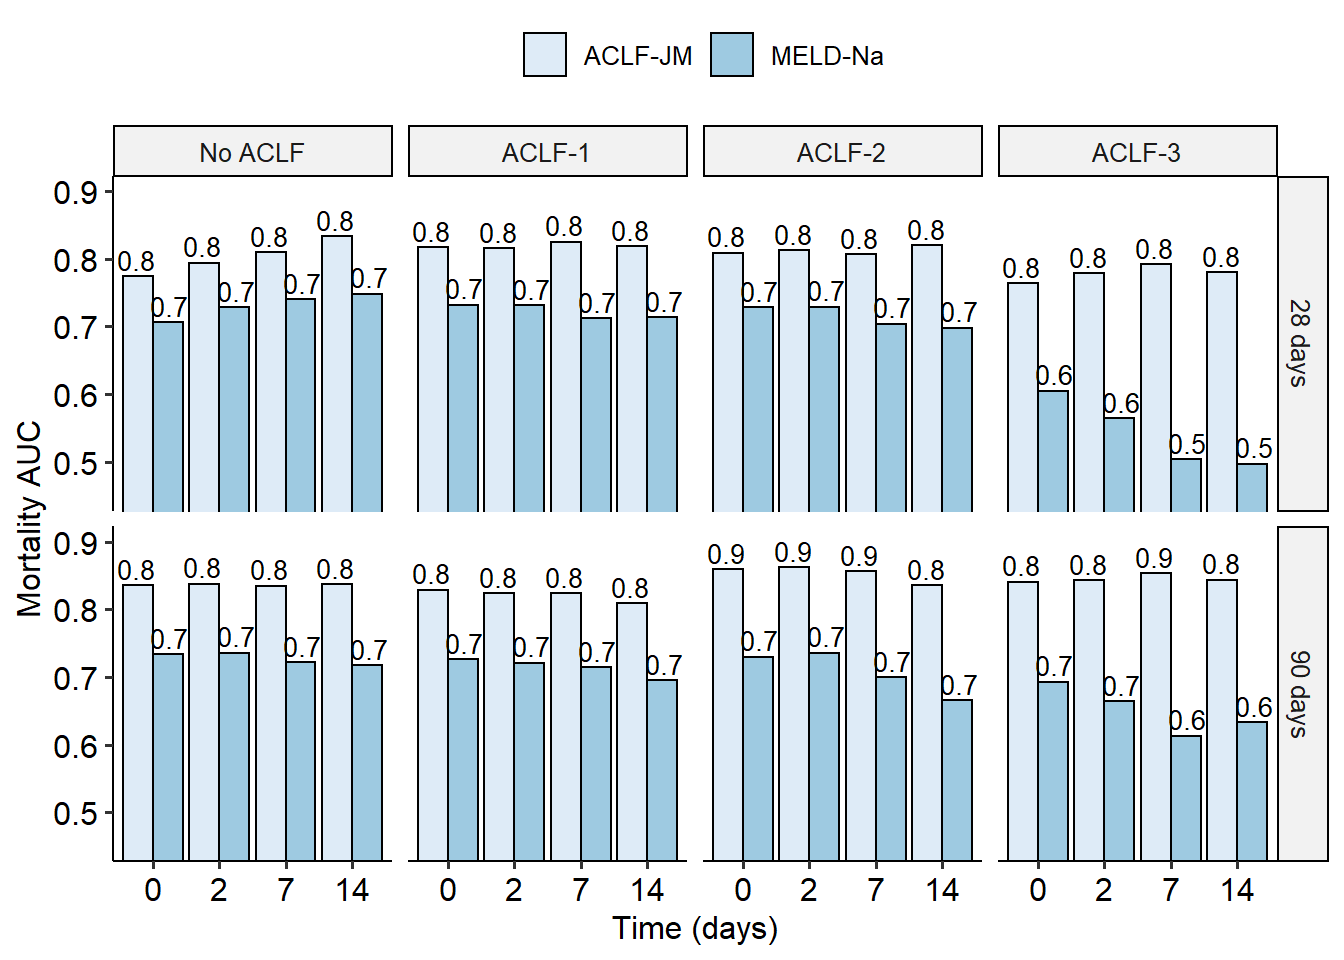
\includegraphics{thesis_files/figure-latex/aclf-fig2-1.pdf}
\caption{\label{fig:aclf-fig2}The AUCs for 28- and 90-day mortality prediction of the ACLF-JM and the MELD-Na, stratified for ACLF severity.}
\end{figure}

Figure \ref{fig:aclf-fig2} show that with increasing ACLF grade, JM performance remains significantly better than the declining MELD-Na (also see table S3 and figure S3). Especially for 90-day prediction in ACLF grade 3 patients, JM performance is excellent with AUCs ranging from 0.841 to 0.853, contrasting the MELD-Na AUCs between 0.613 and 0.693. MELD-Na AUCs (almost) equal chance when predicting 28-day mortality in ACLF-3 patients, ranging from 0.497 to 0.605. Importantly, the ACLF-JM also better estimated risks, i.e.~is better calibrated, than the MELD-Na (figure S2B). With increasing ACLF grade, prediction errors were improved up to 37.6\% (figure S3B). An accurate model is important for clinical decision-making, because decisions are often based on risks.\textsuperscript{19}

\hypertarget{aclf-jm-impact-on-the-transplantation-waiting-list-1}{%
\subsection*{ACLF-JM impact on the transplantation waiting list}\label{aclf-jm-impact-on-the-transplantation-waiting-list-1}}
\addcontentsline{toc}{subsection}{ACLF-JM impact on the transplantation waiting list}

To study the difference in survival prediction and subsequent allocation priority between the ACLF-JM and the MELD-Na, patients were followed the first 28 days. In total, 2636 transplants were done within this period. Figure \ref{fig:aclf-fig3} shows the correlation plot between MELD-Na scores and ACLF-JM mortality estimates after 28 days of waiting list follow-up. For 2186 patients (in green), transplantation priority was given according to both the ACLF-JM and MELD-Na, as estimated mortality without LT was highest. More interestingly, 450 patients (in blue) could possibly have been prioritized by the ACLF-JM, but not by MELD-Na.

\begin{figure}
\centering
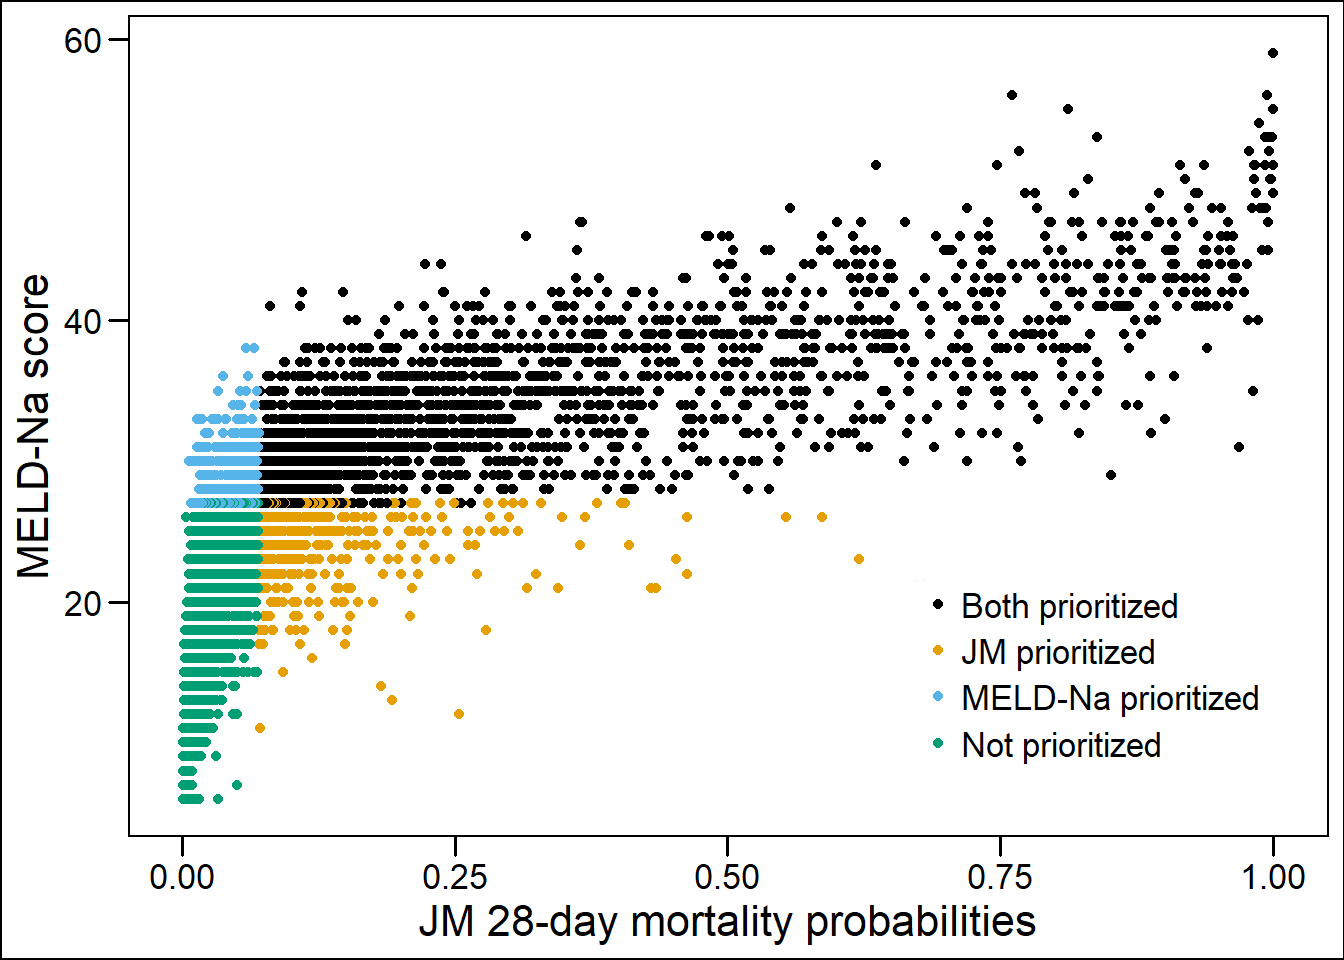
\includegraphics{thesis_files/figure-latex/aclf-fig3-1.pdf}
\caption{\label{fig:aclf-fig3}The correlation plot of MELD-Na score and ACLF-JM 28 days survival predictions. Patients are stratified in 4 groups: orange and blue patients would have been prioritized differently under either the ACLF-JM or MELD-Na. Blue patients had a 4x higher 28-day waiting list mortality than orange patients.}
\end{figure}

Importantly, although these patients had lower median MELD-Na scores, they also had four times higher 28-day mortality rates, i.e., 13.1\% versus 3.1\%, see Table \ref{tab:aclf-tab3}. Compared to the 450 MELD-Na-prioritized patients (orange), ACLF-JM-prioritized patients were older, more often female, had lower ACLF-1 rates, more NASH, less alcohol-induced liver disease and were more often dependent on life-support. After 28 days, 190 patients were delisted due to increased disease severity. In these patients, survival prediction AUC (95\%CI) of the ACLF-JM and MELD-Na was 88.0 (85.1-90.9) and 82.5 (79.0-85.9), respectively (figure S6).

\hypertarget{clinical-application-of-the-aclf-jm-1}{%
\subsection*{Clinical application of the ACLF-JM}\label{clinical-application-of-the-aclf-jm-1}}
\addcontentsline{toc}{subsection}{Clinical application of the ACLF-JM}

After constructing and validating the ACLF-JM in this large cohort, an online application was developed, which allows clinicians to easily calculate individual patient survival probabilities based on the ACLF-JM. Available at: \url{https://predictionmodels.shinyapps.io/aclf-jm/}. Excel files with repeated MELD-Na measurements can be uploaded into this tool, to generate dynamic survival predictions during follow-up. The ACLF-JM simulates individual patient data to calculate personalized predictions. See supplement 1 for precise instructions for the data upload and supplement 2 for a step-by-step manual.

\linespread{1}

\begin{landscape}\begin{table}

\caption{\label{tab:aclf-tab3}Characteristics of patients prioritized differently for liver transplantation within 28 days}
\centering
\resizebox{\linewidth}{!}{
\begin{threeparttable}
\begin{tabular}[t]{llllll}
\toprule
Characteristics & Both prioritized & ACLF-JM prioritized & MELD-Na prioritized & Not prioritized & p*\\
\midrule
\cellcolor{gray!6}{n} & \cellcolor{gray!6}{2186} & \cellcolor{gray!6}{450} & \cellcolor{gray!6}{450} & \cellcolor{gray!6}{6990} & \cellcolor{gray!6}{}\\
Age (median [IQR]) & 56.0 [47.0, 62.0] & 62.0 [55.0, 67.0] & 50.0 [42.0, 56.8] & 59.0 [52.0, 64.0] & <0.001\\
\cellcolor{gray!6}{Male sex (\%)} & \cellcolor{gray!6}{1336 (61.1)} & \cellcolor{gray!6}{175 (38.9)} & \cellcolor{gray!6}{326 (72.4)} & \cellcolor{gray!6}{4552 (65.1)} & \cellcolor{gray!6}{<0.001}\\
Death within 28 days (\%) & 289 (13.2) & 59 (13.1) & 14 (3.1) & 90 (1.3) & <0.001\\
\addlinespace[0.3em]
\multicolumn{6}{l}{\textbf{ACLF (\%)}}\\
\hspace{1em}\cellcolor{gray!6}{No ACLF} & \cellcolor{gray!6}{172 (7.9)} & \cellcolor{gray!6}{191 (42.4)} & \cellcolor{gray!6}{162 (36.0)} & \cellcolor{gray!6}{6155 (88.1)} & \cellcolor{gray!6}{}\\
\hspace{1em}ACLF-1 & 585 (26.8) & 95 (21.1) & 248 (55.1) & 720 (10.3) & \\
\hspace{1em}\cellcolor{gray!6}{ACLF-2} & \cellcolor{gray!6}{792 (36.2)} & \cellcolor{gray!6}{91 (20.2)} & \cellcolor{gray!6}{39 (8.7)} & \cellcolor{gray!6}{105 (1.5)} & \cellcolor{gray!6}{}\\
\hspace{1em}ACLF-3 & 637 (29.1) & 73 (16.2) & 1 (0.2) & 10 (0.1) & \\
\addlinespace[0.3em]
\multicolumn{6}{l}{\textbf{Disease (\%)}}\\
\hspace{1em}\cellcolor{gray!6}{Cirrhosis HCV} & \cellcolor{gray!6}{165 (7.5)} & \cellcolor{gray!6}{31 (6.9)} & \cellcolor{gray!6}{39 (8.7)} & \cellcolor{gray!6}{1099 (15.7)} & \cellcolor{gray!6}{}\\
\hspace{1em}NASH & 392 (17.9) & 147 (32.7) & 61 (13.6) & 1479 (21.2) & \\
\hspace{1em}\cellcolor{gray!6}{Cirrhosis Alcoholic} & \cellcolor{gray!6}{964 (44.1)} & \cellcolor{gray!6}{130 (28.9)} & \cellcolor{gray!6}{235 (52.2)} & \cellcolor{gray!6}{1768 (25.3)} & \cellcolor{gray!6}{}\\
\hspace{1em}Cirrhosis Other & 416 (19.0) & 68 (15.1) & 55 (12.2) & 988 (14.1) & \\
\hspace{1em}\cellcolor{gray!6}{Cholestatic disease} & \cellcolor{gray!6}{104 (4.8)} & \cellcolor{gray!6}{41 (9.1)} & \cellcolor{gray!6}{36 (8.0)} & \cellcolor{gray!6}{638 (9.1)} & \cellcolor{gray!6}{}\\
\hspace{1em}Metabolic disease & 56 (2.6) & 5 (1.1) & 13 (2.9) & 135 (1.9) & \\
\hspace{1em}\cellcolor{gray!6}{Malignant/benign tumor} & \cellcolor{gray!6}{39 (1.8)} & \cellcolor{gray!6}{11 (2.4)} & \cellcolor{gray!6}{7 (1.6)} & \cellcolor{gray!6}{734 (10.5)} & \cellcolor{gray!6}{}\\
\hspace{1em}Other & 50 (2.3) & 17 (3.8) & 4 (0.9) & 149 (2.1) & \\
\cellcolor{gray!6}{MELD (median [IQR])} & \cellcolor{gray!6}{34.0 [29.0, 39.0]} & \cellcolor{gray!6}{24.0 [21.0, 28.0]} & \cellcolor{gray!6}{26.0 [23.0, 29.0]} & \cellcolor{gray!6}{15.0 [11.0, 19.0]} & \cellcolor{gray!6}{<0.001}\\
MELD-Na (median [IQR]) & 33.0 [30.0, 38.0] & 25.0 [23.0, 26.0] & 28.0 [27.0, 30.0] & 15.0 [10.0, 20.0] & <0.001\\
\cellcolor{gray!6}{Life support dependent} & \cellcolor{gray!6}{291 (13.3)} & \cellcolor{gray!6}{84 (18.7)} & \cellcolor{gray!6}{3 (0.7)} & \cellcolor{gray!6}{50 (0.7)} & \cellcolor{gray!6}{<0.001}\\
\bottomrule
\end{tabular}
\begin{tablenotes}
\item \textit{Note: } 
\item Clarification: JM-prioritized patients are not prioritized by MELD-Na, and vice versa.
\item[*] Difference tested between ACLF-JM-prioritized and MELD-Na-prioritized patients
\end{tablenotes}
\end{threeparttable}}
\end{table}
\end{landscape}

\linespread{1.213}

\hypertarget{discussion-3}{%
\section*{Discussion}\label{discussion-3}}
\addcontentsline{toc}{section}{Discussion}

In this study, we developed and validated the ACLF-JM prediction model, to estimate survival of ACLF patients. We report several important findings. First, both current and past disease severity and its rate of change are strongly associated with survival in ACLF. Second, by using these data, the ACLF-JM gives excellent prediction performance, even in ACLF-3, and significantly outperforms MELD-Na. Third, the ACLF-JM could have prioritized patients with low median MELD-Na scores, i.e.~not identified by MELD-Na, but four times higher mortality rates than MELD-Na prioritized patients. Fourth, the ACLF-JM can be clinically applied online to estimate and visualize patient-specific survival, which can be updated with every new measurement.

\hypertarget{disease-development-over-time}{%
\subsection*{Disease development over time}\label{disease-development-over-time}}
\addcontentsline{toc}{subsection}{Disease development over time}

ACLF disease severity is dynamic and can change rapidly. During the first week, disease severity changes for most patients, resulting in different survival outcomes.\textsuperscript{9,10} The current liver allocation system does not consider change, as it uses only the most recent measurement for survival prediction and ignores previous data. Moreover, survival is estimated based on the MELD-Na score, which ignores relevant factors for ACLF and therefore underestimates mortality.\textsuperscript{7,8} Hernaez et al.~showed that mortality was higher than expected in low MELD-Na score patients. They also showed that, despite their high(er) ACLF grade, these low MELD-Na patients were often not considered for LT.\textsuperscript{7} Interestingly, Hernaez et al.~mentioned that ``Future research should also focus on developing and validating prognostic scores that incorporate dynamic changes in patients clinical course,'' i.e.~the goal of this study. Sundaram et al.~showed that ACLF death and removal rate did not correlate well with the MELD-Na score, as mortality rates were highest in ACLF-3 patients with MELD-Na \textless25.\textsuperscript{8} In this study, ACLF was present in 33.3\% of the patients. Therefore, the MELD-Na underestimation of ACLF disease severity could be substantial, which possibly leads to unequal treatment access and surplus mortality.\textsuperscript{7}

Therefore, the ACLF-JM was developed to predict ACLF patient survival based on disease development over time. The model provides several important improvements over the MELD-Na (table S4).\textsuperscript{21} Most importantly, predictions are based on all available previous data and update for every new measurement.\textsuperscript{22} Predictions should be updated based on accumulating evidence, because ACLF is a dynamic disease. Also, the ACLF-JM considers both the value of disease severity and the rate at which disease severity is changing, see Figure \ref{fig:aclf-fig1}. It uses more nuanced aspects of ACLF disease development to predict survival. Thus, like a clinician, past and current disease developments are used to estimate patient prognosis. Updating prognosis is important in ACLF, as disease can increase fast and non-linearly (e.g.~exponential).\textsuperscript{1,3} ACLF-JM survival predictions could therefore be used to aid clinical decision making for ACLF patients on the waiting list for LT, as current models result in unequal transplantation access and post-LT survival rates.\textsuperscript{8,10,17} Furthermore, In this cohort, we showed that ACLF-JM prioritization identified patients with low MELD-Na scores, but high mortality, see Table \ref{tab:aclf-tab3}. Mortality is underestimated in these patients and subsequently they receive a lower priority for LT. Since ACLF patients benefit from fast LT,\textsuperscript{17} use of the ACLF-JM for the evaluation of prognosis could perhaps help to resolve the underestimation of waiting list mortality for ACLF patients.\textsuperscript{7}

\hypertarget{aclf-jm-validation}{%
\subsection*{ACLF-JM validation}\label{aclf-jm-validation}}
\addcontentsline{toc}{subsection}{ACLF-JM validation}

The ACLF-JM showed excellent short-term survival prediction performance at baseline and with increasing follow-up. Increasing ACLF grade did not lead to a decrease in predictive accuracy. This is important, because risk of death and need for LT should be reliably estimated in the sickest patients. Our data showed that both the ACLF-JM and MELD-Na AUCs declined with increasing follow-up. This is likely due to population changes, i.e.~the sickest patients die or are transplanted first and less patients remain with increasing follow-up.\textsuperscript{23} Also, with increasing disease severity, generally a shorter follow-up period is available. The ACLF-JM approximation of disease does not depend on the number of measurements per patient, because it estimates disease over time as a continuous trajectory (figure S4). This is important, because frequency of measurement confounded previous (Cox-based) survival predictions for patients in need of LT.\textsuperscript{24} The ACLF-JM performed comparable and sometimes even better compared to the reported performance of the CLIF-C OF score.\textsuperscript{6} This could possibly indicate that ACLF-JM performance was adequate enough for clinical application. Because the UNOS registry does not contain data on white blood cell counts, CLIF-C ACLF scoring was not possible in this study. ACLF-JM performance could however be externally validated in the cohorts used to construct the CLIF-C scores.\textsuperscript{6}

\hypertarget{clinical-application-of-the-aclf-jm-2}{%
\subsection*{Clinical application of the ACLF-JM}\label{clinical-application-of-the-aclf-jm-2}}
\addcontentsline{toc}{subsection}{Clinical application of the ACLF-JM}

After training and ascertaining excellent performance, an online tool of the ACLF-JM was created for clinical use. Especially in ACLF, both the patient and treating clinician benefit from patient-specific modelling, which shifts the focus of prediction from the population to the individual patient level. Jalan et al.~already stated that there is a need for models that ``update on a daily basis providing additional prognostic information,'' and that ``currently, no validated evidence-based tools guide the decision-making.''\textsuperscript{6} The ACLF-JM meets these demands and more, with excellent performance leading to personalized prediction, readily available online for any clinician.

\hypertarget{limitations-3}{%
\subsection*{Limitations}\label{limitations-3}}
\addcontentsline{toc}{subsection}{Limitations}

A limitation is that longitudinal MELD-Na measurements are not best to model ACLF disease development, as they can underestimate ACLF disease severity.\textsuperscript{7} Ideally, longitudinal CLIF-C ACLFs data would be available in the UNOS data. However, MELD-Na was one of the few consistently available longitudinal measurements, which allowed analysis on a large scale and comparison to previous studies. The retrospective analysis of large databases also has several disadvantages. Misclassification of disease severity could give bias, e.g.~subjective scoring of ascites and encephalopathy. Also, surrogate markers, suggested by authors of other large UNOS ACLF analyses, were used for ventilatory and circulatory failure.\textsuperscript{6,8,10,17} For example, mechanical ventilation was used as replacement for respiratory failure, it is however very well possible that a patient with respiratory failure did not receive mechanical ventilation, or vice versa. Despite these shortcomings, the ACLF-JM showed excellent performance with increasing disease severity (ACLF grade).

\hypertarget{conclusion-3}{%
\section*{Conclusion}\label{conclusion-3}}
\addcontentsline{toc}{section}{Conclusion}

ACLF survival is dynamically predicted by the ACLF-JM prediction model, using both longitudinal and survival data. Updating prognosis on new measurements is important, as ACLF is a dynamic disease. The ACLF-JM prediction performance was excellent in this cohort, even in ACLF-3 patients. The ACLF-JM could therefore be used as a tool for the personalized evaluation of prognosis and clinical decision making in patients with ACLF.

\newpage
\linespread{1}
\small

\hypertarget{references-4}{%
\section*{References}\label{references-4}}
\addcontentsline{toc}{section}{References}

\begin{enumerate}
\def\labelenumi{\arabic{enumi}.}
\tightlist
\item
  Jalan R, Gines P, Olson JC, et al.~Acute-on chronic liver failure. J Hepatol. 2012;57(6):1336-1348. \url{doi:10.1016/j.jhep.2012.06.026}
\item
  Hernaez R, Kramer JR, Liu Y, et al.~Prevalence and short-term mortality of acute-on-chronic liver failure: A national cohort study from the USA. J Hepatol. 2019;70(4):639-647. \url{doi:10.1016/j.jhep.2018.12.018}
\item
  Moreau R, Jalan R, Gines P, et al.~Acute-on-chronic liver failure is a distinct syndrome that develops in patients with acute decompensation of cirrhosis. Gastroenterology. 2013;144(7):1426-1437.e9. \url{doi:10.1053/j.gastro.2013.02.042}
\item
  Kim WR, Biggins SW, Kremers WK, et al.~Hyponatremia and Mortality among Patients on the Liver-Transplant Waiting List. N Engl J Med. 2008;359(10):1018-1026. \url{doi:10.1007/s11250-017-1262-3}
\item
  Goudsmit BFJ, Putter H, Tushuizen ME, et al.~Validation of the Model for End‐stage Liver Disease sodium (MELD‐Na) score in the Eurotransplant region. Am J Transplant. 2020. \url{doi:10.1111/ajt.16142}
\item
  Jalan R, Saliba F, Pavesi M, et al.~Development and validation of a prognostic score to predict mortality in patients with acute-on-chronic liver failure. J Hepatol. 2014;61(5):1038-1047. \url{doi:10.1016/j.jhep.2014.06.012}
\item
  Hernaez R, Liu Y, Kramer JR, Rana A, El-Serag HB, Kanwal F. Model for end-stage liver disease-sodium underestimates 90-day mortality risk in patients with acute-on-chronic liver failure. J Hepatol. 2020:1-9. \url{doi:10.1016/j.jhep.2020.06.005}
\item
  Sundaram V, Jalan R, Wu T, et al.~Factors Associated with Survival of Patients With Severe Acute-On-Chronic Liver Failure Before and After Liver Transplantation. Gastroenterology. 2019;156(5):1381-1391.e3. \url{doi:10.1053/j.gastro.2018.12.007}
\item
  Gustot T, Fernandez J, Garcia E, et al.~Clinical Course of acute-on-chronic liver failure syndrome and effects on prognosis. Hepatology. 2015;62(1):243-252. \url{doi:10.1002/hep.27849}
\item
  Sundaram V, Kogachi S, Wong RJ, et al.~Effect of the clinical course of acute-on-chronic liver failure prior to liver transplantation on post-transplant survival. J Hepatol. 2020;72(3):481-488. \url{doi:10.1016/j.jhep.2019.10.013}
\item
  Rizopoulos R. Joint Models for Longitudinal and Time-to-Event Data: With Applications in R. 1st ed.~Chapman and Hall/CRC; 2012.
\item
  Papageorgiou G, Mokhles MM, Takkenberg JJM, Rizopoulos D. Individualized dynamic prediction of survival with the presence of intermediate events. Stat Med. 2019;38(30):5623-5640. \url{doi:10.1002/sim.8387}
\item
  Arisido MW, Antolini L, Bernasconi DP, Valsecchi MG, Rebora P. Joint model robustness compared with the time-varying covariate Cox model to evaluate the association between a longitudinal marker and a time-to-event endpoint. BMC Med Res Methodol. 2019;19(1):1-13. \url{doi:10.1186/s12874-019-0873-y}
\item
  Campbell KR, Juarez-Colunga E, Grunwald GK, Cooper J, Davis S, Gralla J. Comparison of a time-varying covariate model and a joint model of time-to-event outcomes in the presence of measurement error and interval censoring: Application to kidney transplantation. BMC Med Res Methodol. 2019;19(1):1-12. \url{doi:10.1186/s12874-019-0773-1}
\item
  Hernaez R, Liu Y, Kramer JR, Rana A, El-serag HB, Kanwal F. Model for end-stage liver disease-sodium underestimates 90-day mortality risk in patients with acute-on-chronic liver failuare. J Hepatol. 2020. \url{doi:10.1016/j.jhep.2020.06.005}
\item
  Moons KGM, Altman DG, Reitsma JB, et al.~Transparent reporting of a multivariable prediction model for individual prognosis or diagnosis (TRIPOD): Explanation and elaboration. Ann Intern Med. 2015;162(1):W1-W73. \url{doi:10.7326/M14-0698}
\item
  Thuluvath PJ, Thuluvath AJ, Hanish S, Savva Y. Liver transplantation in patients with multiple organ failures: Feasibility and outcomes. J Hepatol. 2018;69(5):1047-1056. \url{doi:10.1016/j.jhep.2018.07.007}
\item
  Rizopoulos D. The R package jmbayes for fitting joint models for longitudinal and time-to-event data using MCMC. J Stat Softw. 2016;72(7). \url{doi:10.18637/jss.v072.i07}
\item
  Gerds TA, Blanche P, Mortensen R, Tollenaar N, Brasch Mogensen U, Ozenne B. riskRegression: Risk Regression Models and Prediction Scores for Survival Analysis with Competing Risks. 2020. \url{https://cran.r-project.org/web/packages/riskRegression/index.html}.
\item
  Van Calster B, McLernon DJ, Van Smeden M, et al.~Calibration: The Achilles heel of predictive analytics. BMC Med. 2019;17(1):1-7. \url{doi:10.1186/s12916-019-1466-7}
\item
  Goudsmit BFJ, Tushuizen ME, Putter H, Braat AE, van Hoek B. The role of the model for end-stage liver disease-sodium score and joint models for 90-day mortality prediction in patients with acute-on-chronic liver failure. J Hepatol. 2021;74(2):475-476. \url{doi:10.1016/j.jhep.2020.08.032}
\item
  Papageorgiou G, Mauff K, Tomer A, Rizopoulos D. An Overview of Joint Modeling of Time-to-Event and Longitudinal Outcomes. Annu Rev Stat Its Appl. 2019;6(1):223-240. \url{doi:10.1146/annurev-statistics-030718-105048}
\item
  Goudsmit BFJ, Putter H, Tushuizen ME, et al.~Refitting the model for end-stage liver disease for the Eurotransplant region. Hepatology. 2020;in press.
\end{enumerate}

\newpage
\linespread{1.213}
\normalsize
\thispagestyle{plain}

\mbox{}

\pagecolor{black}
\color{white}

\hypertarget{part-iii-survival-with-and-without-transplantation}{%
\chapter*{Part III: Survival with and without transplantation}\label{part-iii-survival-with-and-without-transplantation}}
\addcontentsline{toc}{chapter}{Part III: Survival with and without transplantation}

\begin{quote}
``\emph{What can be controlled is never completely real;}
\end{quote}

\begin{quote}
\emph{what is real can never be completely controlled.''}
\end{quote}

\begin{quote}
--- Vladimir Nabokov
\end{quote}

\begin{center}\rule{0.5\linewidth}{0.5pt}\end{center}

\newpage

\hypertarget{chap-benefit}{%
\chapter{Survival benefit from liver transplantation for patients with and without hepatocellular carcinoma}\label{chap-benefit}}

\chaptermark{Benefit from LT}

\vspace*{\fill}

\noindent 
Goudsmit BFJ, Prosepe I, Tushuizen ME, et al.~Survival benefit from liver transplantation for patients with and without hepatocellular carcinoma. \emph{Under review.}

\begin{center}\rule{0.5\linewidth}{0.5pt}\end{center}

\newpage
\nopagecolor
\color{black}

\noindent 
\small

\textbf{Abstract}

\textbf{Background \& Aims}: In the US, inequal liver transplantation (LT) access exists between patients with and without hepatocellular carcinoma (HCC). Survival benefit considers survival without and with LT and could equalize LT access. We calculated and compared LT survival benefit scores for patients with(out) HCC, based on longitudinal data in a recent US cohort.

\textbf{Methods}: Adult LT candidates with(out) HCC between 2010-2019 were included. Waitlist survival over time was contrasted to posttransplant survival, to estimate 5-year survival benefit from the moment of LT. Waitlist survival was modeled with bias-corrected time-dependent Cox regression and posttransplant survival was estimated through Cox proportional hazards regression.

\textbf{Results}: Mean HCC survival without LT was always lower than non-HCC waitlist survival. Below MELD(-Na) 30, HCC patients gained more life-years from LT than non-HCC patients at the same MELD(-Na) score. Only non-HCC patients below MELD(-Na) 9 had negative benefit. Most HCC patients were transplanted below MELD(-Na) 14 and most non-HCC patients above MELD(-Na) 26. Liver function (MELD(-Na), albumin) was the main predictor of 5-year benefit. Therefore, during five years, most HCC patients gained 0.12 to 1.96 years from LT, whereas most non-HCC patients gained 2.48 to 3.45 years.

\textbf{Conclusion}: On an individual level, transplanting patients with HCC resulted in survival benefit. However, on a population level, benefit was indirectly wasted, as non-HCC patients were likely to gain more survival due to decreased liver function. Based on these data, we now provide an online calculator to estimate 5-year survival benefit given specific patient characteristics. Survival benefit scores could serve to equalize LT access.

\linespread{1.213}
\normalsize
\newpage

\hypertarget{introduction-4}{%
\section*{Introduction}\label{introduction-4}}
\addcontentsline{toc}{section}{Introduction}

Adult liver transplantation (LT) relies on scarce donor grafts. Therefore, allocation prioritizes patients that likely will die soon without transplantation.\textsuperscript{1} For most patients on the LT waiting list in the United States (US), the Model for End-stage Liver Disease sodium (MELD-Na) score adequately predicts expected survival without transplantation.\textsuperscript{2,3}

However, MELD-Na is less predictive of survival for transplant candidates with hepatocellular carcinoma (HCC). This is because HCC mortality is typically caused by tumor progression and not by liver failure.\textsuperscript{4} The number of HCC patients listed for transplantation has tripled the past 10 years.\textsuperscript{5} HCC is the single most important cause of death in cirrhotic patients, and treatment through LT still has the best long-term results.\textsuperscript{6--8} The exception point system was developed to compensate liver graft allocation based on inadequate MELD(-Na) survival prediction for most notably HCC patients. In this system, HCC patients receive artificial MELD points that increase automatically every 90 days, to mimic HCC progression.\textsuperscript{9--11} Unintendedly, the exception points created inequity between non-HCC and HCC patients, because HCC LT access increased too much,\textsuperscript{12--14} and inequity among HCC patients, because all patients within one region receive the same priority with only waiting time as tiebreaker.\textsuperscript{15}

Instead of arbitrary points, patient characteristics should be used to model the risk of waiting list dropout.\textsuperscript{10,14,16--18} Moreover, to balance the principles urgency and utility,\textsuperscript{19} the risk of waiting list dropout should be compared to expected post-transplant survival. The difference is survival benefit, or the life-years gained from transplantation.\textsuperscript{20} Considering LT survival benefit is valuable because donor grafts are scarce and some patients gain more life-years than others.\textsuperscript{20--23}

Benefit of non-HCC and HCC patients has been previously evaluated,\textsuperscript{13,14,16,17} but re-evaluation is warranted. Firstly, because contradicting findings have been reported. Most notably, Vitale et al.~showed that HCC patients in Italy benefited twice as much from LT compared to non-HCC patients,\textsuperscript{17} whereas Berry et al.~stated that US HCC patients derived negative or little benefit.\textsuperscript{13} Secondly, previous work defined survival benefit as the difference between post-transplant survival and waiting list survival counted from first registration. We hypothesized that counting waiting list survival from first registration is suboptimal, as LT candidates on average have to wait six to eight months for transplantation.\textsuperscript{5} During this time, liver disease will typically progress,\textsuperscript{24,25} patients can drop out,\textsuperscript{5} or HCC could be downstaged.\textsuperscript{6} This changes survival rates as compared to baseline.\textsuperscript{20,21,23,26} Because survival is gained from the moment of possible transplantation, benefit should be counted from that moment on, see Figure \ref{fig:benefit-fig1a}. Lastly, benefit evaluation reflective of the current US population and allocation is missing.

\begin{figure}
\centering
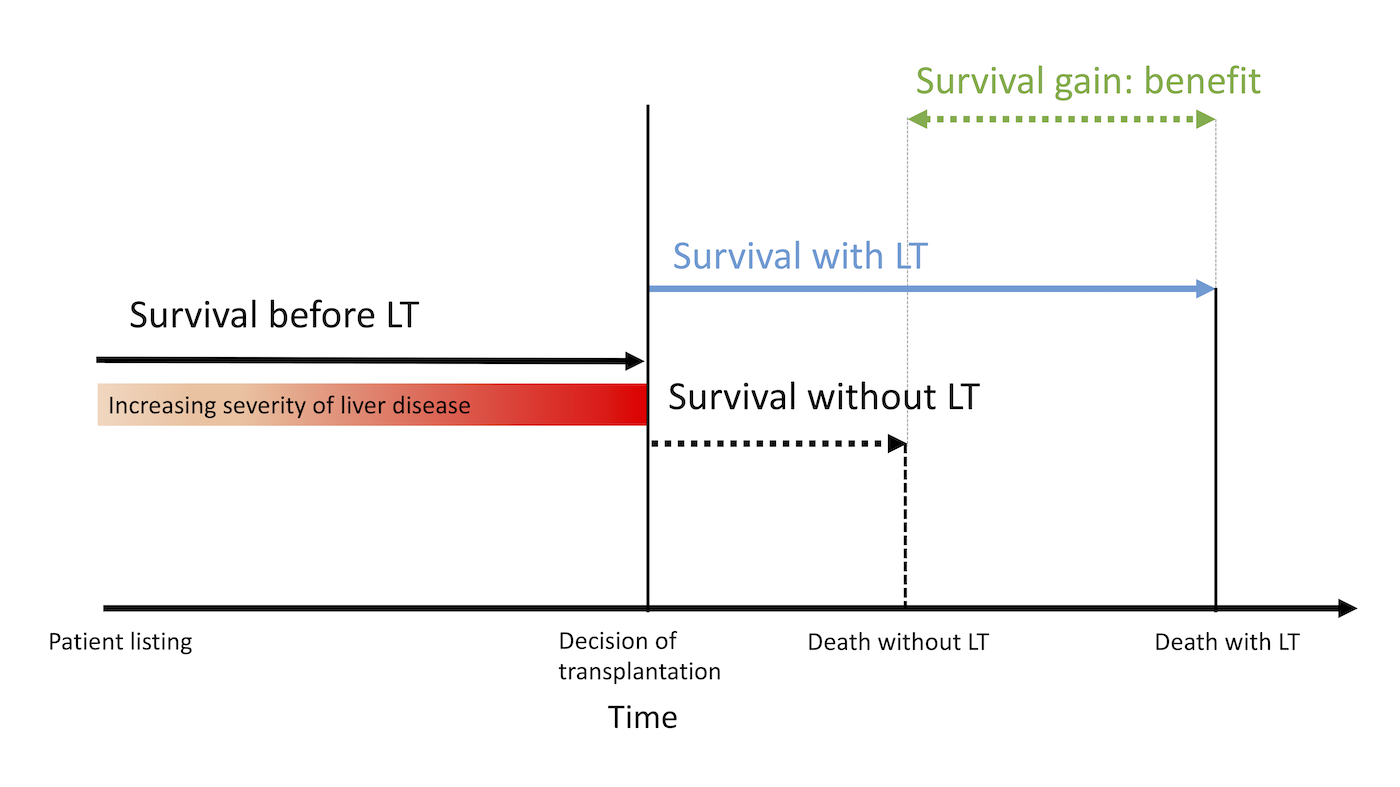
\includegraphics{figures/benefit/figure 1a.pdf}
\caption{\label{fig:benefit-fig1a}Survival benefit is defined as the difference in 5-year life-expectancy with and without transplantation. While patients are waiting for LT, time passes and disease severity typically changes. At the moment of transplantation, benefit is estimated. The survival up until transplantation (`survival before LT') is used to predict waiting list survival in absence of transplantation (`survival without LT'). Without LT survival is then contrasted to posttransplant survival (`with LT') to calculate benefit.}
\end{figure}

Therefore, the goal of this study was to estimate survival gain from transplantation in a large and recent US cohort. We compared LT survival benefit between non-HCC and HCC patients. Life expectancy with transplantation was contrasted to life expectancy without transplantation. We constructed an online benefit application that calculates life expectancy gained from transplantation based on specified patient characteristics.

\hypertarget{methods-4}{%
\section*{Methods}\label{methods-4}}
\addcontentsline{toc}{section}{Methods}

\hypertarget{patient-population}{%
\subsection*{Patient population}\label{patient-population}}
\addcontentsline{toc}{subsection}{Patient population}

This retrospective cohort analysis included adult (\textgreater=18 years) patients listed for a first LT between January 1\textsuperscript{st}, 2010 and April 30\textsuperscript{th}, 2019 on the UNOS waiting list (Figure S1). This interval ended before the May 14\textsuperscript{th}, 2019 implementation of median MELD at transplant.\textsuperscript{15} It also compromised the most recent data with adequate 5-year follow-up completeness. We aimed to calculate benefit for two patient groups: patients without HCC and without exception points (non-HCC group), and patients with HCC and with exception points (HCC group). Although other diseases also qualify for exception points, like primary sclerosing cholangitis and biliary cirrhosis, we only assessed HCC patients, as this is by far the largest group and incidence is increasing.\textsuperscript{5} Current OPTN policy allows standard exception points for 1) HCC patients within Milan criteria (henceforth T2 HCC),\textsuperscript{27} and 2) HCC patients initially outside Milan criteria but successfully downstaged within criteria through loco-regional treatment before LT (henceforth HCC outside criteria). Although previous study found that outcomes of these groups were similar,\textsuperscript{28} we separately analyzed these groups, as the initial HCC disease severity and non-LT treatment are different. We excluded patients with previous LT, acute liver failure, listing for living donation, listing for multiple organs, and non-HCC malignancy (Figure S1). We randomly split our population in training data (67\% of patients) and validation data (the remaining 33\% of patients).

\begin{figure}
\centering
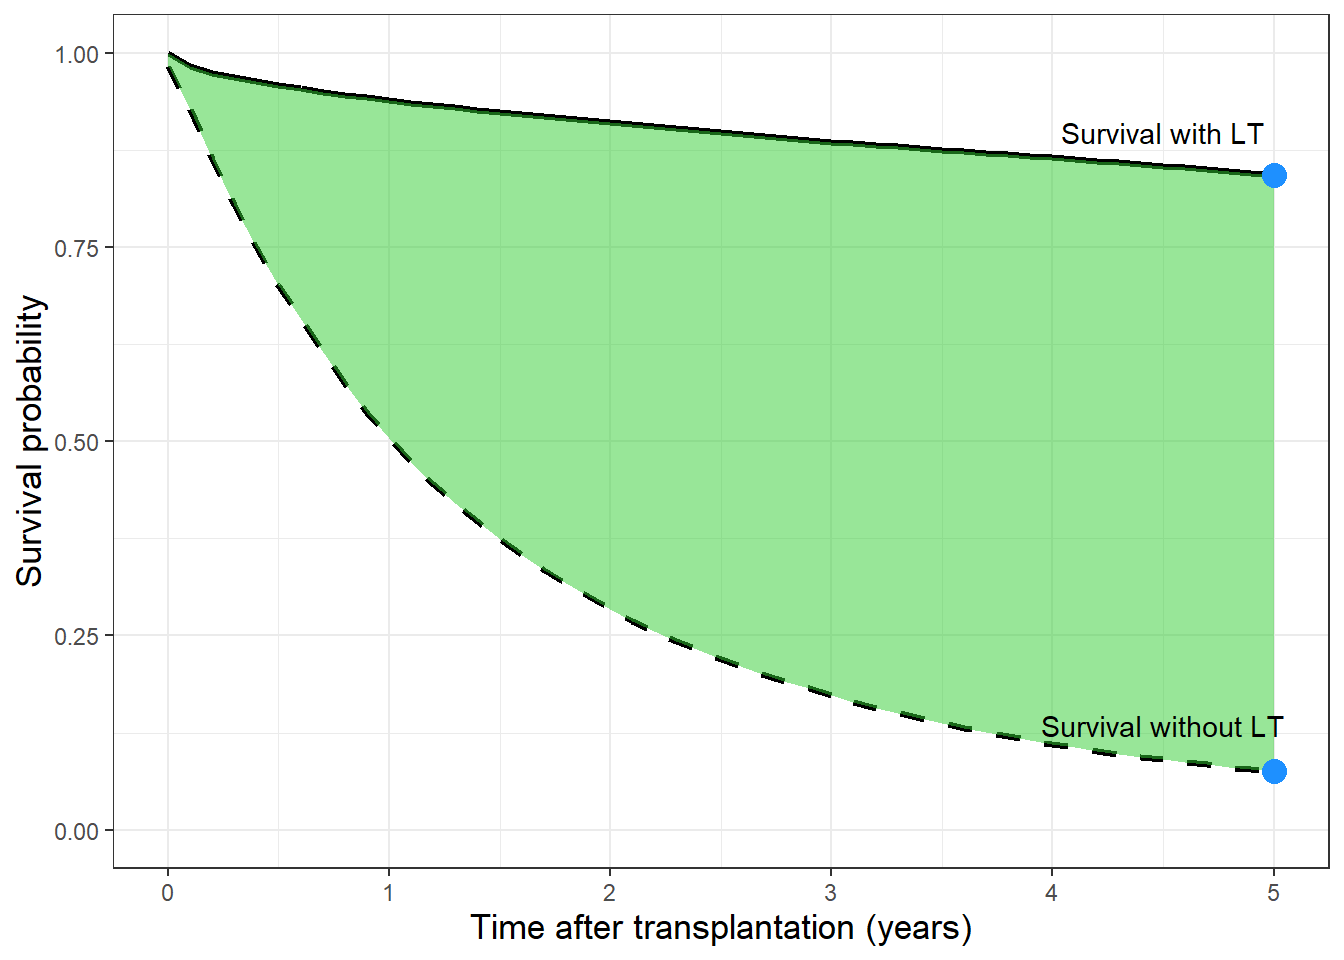
\includegraphics{thesis_files/figure-latex/benefit-fig1b-1.pdf}
\caption{\label{fig:benefit-fig1b}The survival with (solid line), without (dashed line) and benefit from transplantation (green area) are shown. In this example, survival is averaged for non-HCC patients with MELD-Na 25. Please note the difference in survival during five years (lines) and at five years (dots).}
\end{figure}

\hypertarget{benefit-definition}{%
\subsection*{Benefit definition}\label{benefit-definition}}
\addcontentsline{toc}{subsection}{Benefit definition}

Survival benefit was defined as the life-years gained from transplantation during the next five years, see Figure \ref{fig:benefit-fig1b}.\textsuperscript{21,29} To estimate benefit for a given transplanted patient, post-transplantation survival (henceforth `with LT') was contrasted to the hypothetical waiting list survival if LT would not have happened (henceforth `without LT'), again see Figure \ref{fig:benefit-fig1a}.\textsuperscript{21}

Crucially, we estimated future waiting list survival from the moment of LT and not from baseline, as patients are not transplanted at baseline. To model without LT survival, we chose time-dependent Cox regression corrected with inverse probability censoring weighting (IPCW), in accordance to previous studies.\textsuperscript{21--23,26} IPCW is used when treatment is initiated after baseline and the chance of treatment depends on patient characteristics, that is changing MELD-Na scores over time.\textsuperscript{21,26,30} This dependence confounds analysis of waiting list survival upon which allocation is based. These risks therefore must be corrected with statistical methods, preferably IPCW.\textsuperscript{21,26,30} Unlike previous work,\textsuperscript{13,16,17,28,31,32} we specifically did not use intention-to-treat (ITT) or competing risk analysis, please see supplement 1 for a detailed explanation. In short, because 1) they predict a different risk than without LT survival, 2) could result in undertreatment of patients,\textsuperscript{30} and 3) we wanted to model changes in waiting list disease over time beyond baseline. The IPCW analyses are more complex and therefore less often applied, but this does not mean we should not use them.\textsuperscript{33}

\hypertarget{statistical-analysis-2}{%
\subsection*{Statistical analysis}\label{statistical-analysis-2}}
\addcontentsline{toc}{subsection}{Statistical analysis}

\hypertarget{waiting-list-survival}{%
\subsubsection*{Waiting list survival}\label{waiting-list-survival}}
\addcontentsline{toc}{subsubsection}{Waiting list survival}

The waiting list population was divided in biweekly cross-sections, because in allocation liver grafts are offered to active patients on the waiting list at a certain date, not whole study cohorts of patients.\textsuperscript{21} In time-dependent Cox analysis, repeated MELD-Na scores were modeled over time. Date and type of pre-LT HCC treatments were specifically included to account for their effects on waiting list survival. Additional predictors were used to correct the longitudinal data (Table S1), which we selected from available UNOS candidate variables deemed clinically relevant in published studies.\textsuperscript{10,16--18,21} We excluded some variables a priori, because they referred to pediatric recipients, exclusion criteria, or donor characteristics. The outcome of analysis was waiting list mortality, which comprised death while awaiting LT and removal because of worsened condition. We censored for all other outcomes (e.g., transplantation, removal due to recovery, end of study) and corrected for dependent censoring with IPCW. Through IPCW we also estimated without LT survival of transplanted patients based on logic continuation of disease trajectories of similar patients at the same moment in time that were not transplanted (yet), please see supplement 1 for further explanation.

\hypertarget{post-transplantation-survival}{%
\subsubsection*{Post-transplantation survival}\label{post-transplantation-survival}}
\addcontentsline{toc}{subsubsection}{Post-transplantation survival}

We then used Cox proportional hazards regression to model post-transplant survival. Predictors were selected by assessing relations of available UNOS recipient and donor variables to 5-year survival in univariate models, with backwards selection of significant variables in multivariate analysis. The outcome was 5-year post-transplant survival, defined as the difference between the date of transplantation and the earliest date of death, loss to follow-up or end of study on April 30\textsuperscript{th}, 2019.

\hypertarget{calculating-benefit-scores}{%
\subsubsection*{Calculating benefit scores}\label{calculating-benefit-scores}}
\addcontentsline{toc}{subsubsection}{Calculating benefit scores}

After establishing the Cox models in the training data, 5-year survival benefit from LT was calculated for each transplanted patient in the independent validation data. Benefit scores were averaged per biochemical MELD or MELD-Na {[}MELD(-Na){]} score at transplantation, respectively for transplantations before or after January 11\textsuperscript{th}, 2016, and stratified for non-HCC and HCC patients. We visualized benefit with smoothed general additive model plots per MELD(-Na) score and (non-)HCC disease. We assessed model discrimination for 5-year survival by calculating the area under the receiver-operating-curve (AUC). Cox proportional hazards model calibration (i.e., model accuracy) at five years was assessed based on bootstrapping with 200 repetitions, to obtain overfitting-corrected estimates of predicted survival, which were compared to observed survival probabilities.\textsuperscript{34}

\hypertarget{online-benefit-score-calculator}{%
\subsection*{Online benefit score calculator}\label{online-benefit-score-calculator}}
\addcontentsline{toc}{subsection}{Online benefit score calculator}

It was of interest to calculate LT benefit scores based on individual patient and donor characteristics. These benefit predictions had to be readily available online for the clinician and patient, in an intuitive calculator. Therefore, we fit a regression model to the previously calculated 5-year survival benefit scores. To compromise clinical ease of use and predictive power, only the most predictive variables were used in the benefit regression model. Variable importance for benefit prediction was assessed based on ANOVA tests. We used the overfitting-corrected R\textsuperscript{2} to assess how much variation in benefit was explained by the predictors.\textsuperscript{34} A R\textsuperscript{2} value of 1 indicates that all variability in predictions is accounted for and a value above 0.9 therefore indicates excellent model predictions. The online calculator also gives graphical summaries of benefit, averaged per MELD-Na score and (non-)HCC disease, to illustrate the gain of life years during the next five years.

\hypertarget{results-4}{%
\section*{Results}\label{results-4}}
\addcontentsline{toc}{section}{Results}

\hypertarget{patient-characteristics-at-transplantation}{%
\subsection*{Patient characteristics at transplantation}\label{patient-characteristics-at-transplantation}}
\addcontentsline{toc}{subsection}{Patient characteristics at transplantation}

Characteristics for non-HCC and HCC patients at transplantation between 2010-2019 are shown in Table \ref{tab:benefit-tab1} . Compared to non-HCC patients, HCC patients were slightly older, more often male, and less often of white race/ethnicity. HCC patients also more frequently had diabetes mellitus, were less dependent on renal replacement therapy, and had lower median MELD(-Na) scores. HCC patients were mostly transplanted in medium (2, 4, 6, 7, and 8) and long (1, 5, and 9) UNOS waiting time regions, whereas non-HCC patients were mostly transplanted in short (3, 10, and 11) waiting time regions. Until the moment of transplantation, the vast majority (93\%) of HCC patients were at home and therefore significantly less often in hospital or ICU than non-HCC patients. Accordingly, non-HCC patients were more often dependent on life-support. Median MELD-Na scores in non-HCC, T2 HCC, and HCC beyond criteria patients were 25, 12, and 11, respectively.
The AFP at transplantation for within Milan/T2 criteria and initially outside Milan/T2 criteria HCC patients was on average (SD) 67 (294) and 61 (262) ng/mL, respectively. The average AFP levels were higher in T2 HCC patients than HCC patients beyond criteria, which was likely due to the higher frequency of downstaging non-LT treatment. At time of transplantation, HCC outside criteria patients more frequently had two or three tumors. Average total tumor diameter for T2 and non-T2 HCC was 2.79 (1.11) cm and 3.17 (1.89) cm, respectively.
Donor risk index scores were comparable for (non-)HCC patients, therefore HCC patients on average received the same donor quality organs as non-HCC patients.

\linespread{1}
\small

\begin{landscape}
\begin{ThreePartTable}
\begin{TableNotes}
\item \textit{Note: } 
\item HCC: hepatocellular carcinoma, AFP: alpha-fetoprotein, TTD: total tumor diameter, DRI: donor risk index
\item[*] Long wait time is UNOS regions 1, 5, and 9; mid wait time is regions 2, 4, 6, 7, and 8; and short-wait time is regions 3, 10, and 11.
\end{TableNotes}
\begin{longtable}[t]{lllll}
\caption{\label{tab:benefit-tab1}Recipient and donor characteristics at transplantation between 2010-2019}\\
\toprule
Characteristics & No HCC & T2 HCC & HCC outside criteria & p\\
\midrule
\endfirsthead
\caption[]{\label{tab:benefit-tab1}Recipient and donor characteristics at transplantation between 2010-2019 \textit{(continued)}}\\
\toprule
Characteristics & No HCC & T2 HCC & HCC outside criteria & p\\
\midrule
\endhead

\endfoot
\bottomrule
\insertTableNotes
\endlastfoot
\cellcolor{gray!6}{n} & \cellcolor{gray!6}{24503} & \cellcolor{gray!6}{6922} & \cellcolor{gray!6}{5448} & \cellcolor{gray!6}{}\\
Age (median [IQR]) & 56.0 [48.0, 62.0] & 60.0 [56.0, 65.0] & 62.0 [58.0, 65.0] & <0.001\\
\cellcolor{gray!6}{Female sex (\%)} & \cellcolor{gray!6}{8926 (36.4)} & \cellcolor{gray!6}{1614 (23.3)} & \cellcolor{gray!6}{1133 (20.8)} & \cellcolor{gray!6}{<0.001}\\
\addlinespace[0.3em]
\multicolumn{5}{l}{\textbf{Race/ethnicity (\%)}}\\
\hspace{1em}White & 18897 (77.1) & 4907 (70.9) & 3705 (68.0) & \\
\hspace{1em}\cellcolor{gray!6}{Black} & \cellcolor{gray!6}{1956 (8.0)} & \cellcolor{gray!6}{683 (9.9)} & \cellcolor{gray!6}{542 (9.9)} & \cellcolor{gray!6}{}\\
\hspace{1em}Hispanic & 2790 (11.4) & 873 (12.6) & 782 (14.4) & \\
\hspace{1em}\cellcolor{gray!6}{Other} & \cellcolor{gray!6}{860 (3.5)} & \cellcolor{gray!6}{459 (6.6)} & \cellcolor{gray!6}{419 (7.7)} & \cellcolor{gray!6}{}\\
BMI (median [IQR]) & 28.0 [25.0, 33.0] & 28.0 [25.0, 32.0] & 28.0 [25.0, 32.0] & NS\\
\addlinespace[0.3em]
\multicolumn{5}{l}{\textbf{Indication for transplantation (\%)}}\\
\hspace{1em}\cellcolor{gray!6}{Alcoholic} & \cellcolor{gray!6}{6938 (28.3)} & \cellcolor{gray!6}{-} & \cellcolor{gray!6}{-} & \cellcolor{gray!6}{}\\
\hspace{1em}Cholestatic & 2805 (11.4) & - & - & \\
\hspace{1em}\cellcolor{gray!6}{Hepatitis C virus} & \cellcolor{gray!6}{4666 (19.0)} & \cellcolor{gray!6}{-} & \cellcolor{gray!6}{-} & \cellcolor{gray!6}{}\\
\hspace{1em}NASH & 4688 (19.1) & - & - & \\
\hspace{1em}\cellcolor{gray!6}{Other} & \cellcolor{gray!6}{5406 (22.1)} & \cellcolor{gray!6}{-} & \cellcolor{gray!6}{-} & \cellcolor{gray!6}{}\\
\hspace{1em}T2 HCC & - & 6922 (100) & - & \\
\hspace{1em}\cellcolor{gray!6}{HCC outside criteria} & \cellcolor{gray!6}{-} & \cellcolor{gray!6}{-} & \cellcolor{gray!6}{5448 (100)} & \cellcolor{gray!6}{}\\
Diabetes (\%) & 6113 (24.9) & 2237 (32.3) & 1863 (34.2) & <0.001\\
\cellcolor{gray!6}{Dialysis  (\%)} & \cellcolor{gray!6}{3505 (14.3)} & \cellcolor{gray!6}{119 (1.7)} & \cellcolor{gray!6}{59 (1.1)} & \cellcolor{gray!6}{<0.001}\\
MELD score (median [IQR]) & 25.0 [18.0, 33.0] & 12.0 [9.0, 16.0] & 11.0 [8.0, 14.0] & <0.001\\
\cellcolor{gray!6}{MELD-Na score (median [IQR])} & \cellcolor{gray!6}{27.0 [20.0, 34.0]} & \cellcolor{gray!6}{13.0 [9.0, 17.0]} & \cellcolor{gray!6}{11.0 [8.0, 16.0]} & \cellcolor{gray!6}{<0.001}\\
\addlinespace[0.3em]
\multicolumn{5}{l}{\textbf{Region waiting time* (\%)}}\\
\hspace{1em}long & 4614 (18.8) & 1643 (23.7) & 1401 (25.7) & \\
\hspace{1em}\cellcolor{gray!6}{medium} & \cellcolor{gray!6}{9135 (37.3)} & \cellcolor{gray!6}{3093 (44.7)} & \cellcolor{gray!6}{2255 (41.4)} & \cellcolor{gray!6}{}\\
\hspace{1em}short & 10754 (43.9) & 2186 (31.6) & 1792 (32.9) & \\
\addlinespace[0.3em]
\multicolumn{5}{l}{\textbf{Location (\%)}}\\
\hspace{1em}\cellcolor{gray!6}{home} & \cellcolor{gray!6}{14142 (57.7)} & \cellcolor{gray!6}{6385 (92.2)} & \cellcolor{gray!6}{5124 (94.1)} & \cellcolor{gray!6}{}\\
\hspace{1em}hospital & 6423 (26.2) & 392 (5.7) & 251 (4.6) & \\
\hspace{1em}\cellcolor{gray!6}{ICU} & \cellcolor{gray!6}{3938 (16.1)} & \cellcolor{gray!6}{145 (2.1)} & \cellcolor{gray!6}{73 (1.3)} & \cellcolor{gray!6}{}\\
Life-support (\%) & 2251 (9.2) & 79 (1.1) & 39 (0.7) & <0.001\\
\cellcolor{gray!6}{AFP in ng/mL (mean (SD))} & \cellcolor{gray!6}{-} & \cellcolor{gray!6}{67 (294)} & \cellcolor{gray!6}{61 (262)} & \cellcolor{gray!6}{<0.001}\\
\addlinespace[0.3em]
\multicolumn{5}{l}{\textbf{Number of HCC lesions (\%)}}\\
\hspace{1em}1 & - & 74.2 & 65.5 & \\
\hspace{1em}\cellcolor{gray!6}{2} & \cellcolor{gray!6}{-} & \cellcolor{gray!6}{19.3} & \cellcolor{gray!6}{24.6} & \cellcolor{gray!6}{}\\
\hspace{1em}3 & - & 6.5 & 9.9 & \\
\cellcolor{gray!6}{TTD (mean (SD))} & \cellcolor{gray!6}{-} & \cellcolor{gray!6}{2.79 (1.11)} & \cellcolor{gray!6}{3.17 (1.89)} & \cellcolor{gray!6}{<0.001}\\
DRI (median [IQR]) & 1.35 [1.11, 1.64] & 1.36 [1.11, 1.65] & 1.37 [1.11, 1.65] & NS\\*
\end{longtable}
\end{ThreePartTable}
\end{landscape}

\linespread{1.213}
\normalsize

\hypertarget{waiting-list-survival-model}{%
\subsection*{Waiting list survival model}\label{waiting-list-survival-model}}
\addcontentsline{toc}{subsection}{Waiting list survival model}

The significant predictors of the waiting list Cox model are shown in Table S1. In summary, the most important predictors of survival without LT were age, MELD(-Na) score, serum sodium, serum AFP, serum albumin, presence of diabetes mellitus, presence of ascites, and liver disease etiology. By correcting coefficients through IPCW, the importance of MELD(-Na) increased (data not shown), which was expected as we aimed to correct for dependent censoring bias.

\hypertarget{post-transplantation-survival-model}{%
\subsection*{Post-transplantation survival model}\label{post-transplantation-survival-model}}
\addcontentsline{toc}{subsection}{Post-transplantation survival model}

The significant predictors for the post-transplantation survival model are shown in Table S2. Most important were age, liver disease etiology, being of black race/ethnicity, presence of diabetes mellitus, mechanical ventilation, total tumor diameter, serum AFP, and DRI score. HCC patients with MELD(-Na)\textgreater19, AFP\textgreater24 ng/mL, and total tumor diameter\textgreater3.2 cm had the worst posttransplant 5-year survival rates (58.1\%; 95\% CI 50.2-67.2). For all other HCC patients, 5-year survival was above 60\% (Figure S2).\textsuperscript{29} Post-transplant model AUC of 5-year survival was 61.9 (61.2-62.6), indicating respectable discrimination. More importantly,\textsuperscript{35} model calibration was excellent (Figure S3), which meant that our predicted risks closely resembled observed risks. After establishing model accuracy, survival estimates and benefit were calculated in the validation data.

\hypertarget{survival-without-and-with-lt}{%
\subsection*{Survival without and with LT}\label{survival-without-and-with-lt}}
\addcontentsline{toc}{subsection}{Survival without and with LT}

The distribution of MELD(-Na) scores at transplantation is shown in Figure \ref{fig:benefit-fig2}. Non-HCC patients were mostly transplanted at MELD(-Na) scores above 14 and HCC patients mostly below MELD(-Na) 14. This distribution is important for the interpretation of the survival and benefit estimates presented below.

\begin{figure}
\centering
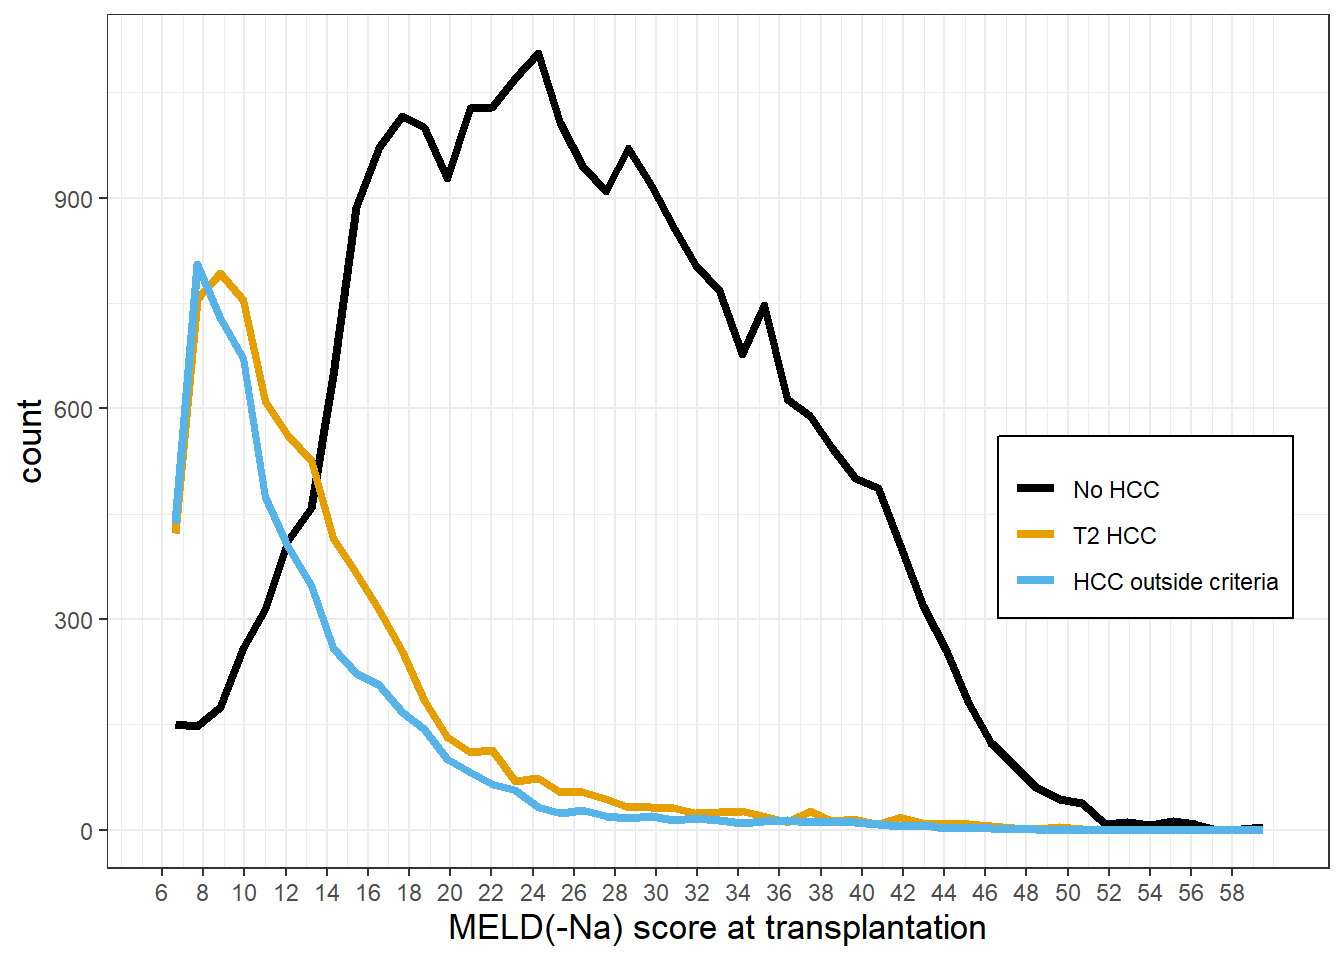
\includegraphics{thesis_files/figure-latex/benefit-fig2-1.pdf}
\caption{\label{fig:benefit-fig2}Distribution of MELD(-Na) scores at transplantation, per (non-)HCC disease. Non-HCC patients are mostly transplanted at MELD(-Na) scores \textgreater14. On the other hand, HCC patients are mostly transplanted below MELD(-Na) 14. Also, a significant part of non-HCC patients is transplanted above MELD(-Na) 30, whereas only 3\% of HCC patients is transplanted at MELD(-Na) above 30.}
\end{figure}

Figure \ref{fig:benefit-fig3a}A shows the smoothed average survival probabilities during the next five years, both for post-transplantation (with LT: solid lines) and for remaining on the waiting list (without LT: dashed lines). Because life years are gained over time, Figure \ref{fig:benefit-fig3a}A shows the mean survival during five years, i.e., the mean of the lines shown in Figure \ref{fig:benefit-fig1b}. The survival probabilities at five years without and with LT are presented in Table S3, which are perhaps more intuitive survival measures for the clinician and patient. However, these hold no information regarding the survival trajectory during five years, which is what the average survival and benefit do encompass.
For non-HCC patients below MELD(-Na) 10, i.e., a small number of patients, see Figure \ref{fig:benefit-fig2}, mean survival probability without LT was better than with LT survival. In other words, on average these patients should not be transplanted. At equal MELD(-Na) scores, waiting list survival without LT for HCC patients was notably lower than for non-HCC patients. Survival without LT probabilities converged at the lowest levels, i.e., mortality could not increase much more at high MELD(-Na) scores. The average survival with LT in both groups declined above approximately MELD(-Na) 24. However, HCC survival decreased more at higher MELD(-Na) scores, most for HCC outside criteria. This decrease in posttransplant survival was possibly due to disease recurrence.

\begin{figure}
\subfloat[The mean survival during the next five years per MELD(-Na) score, for the waiting list (dashed lines) and after transplantation (solid lines).\label{fig:benefit-fig3a-1}]{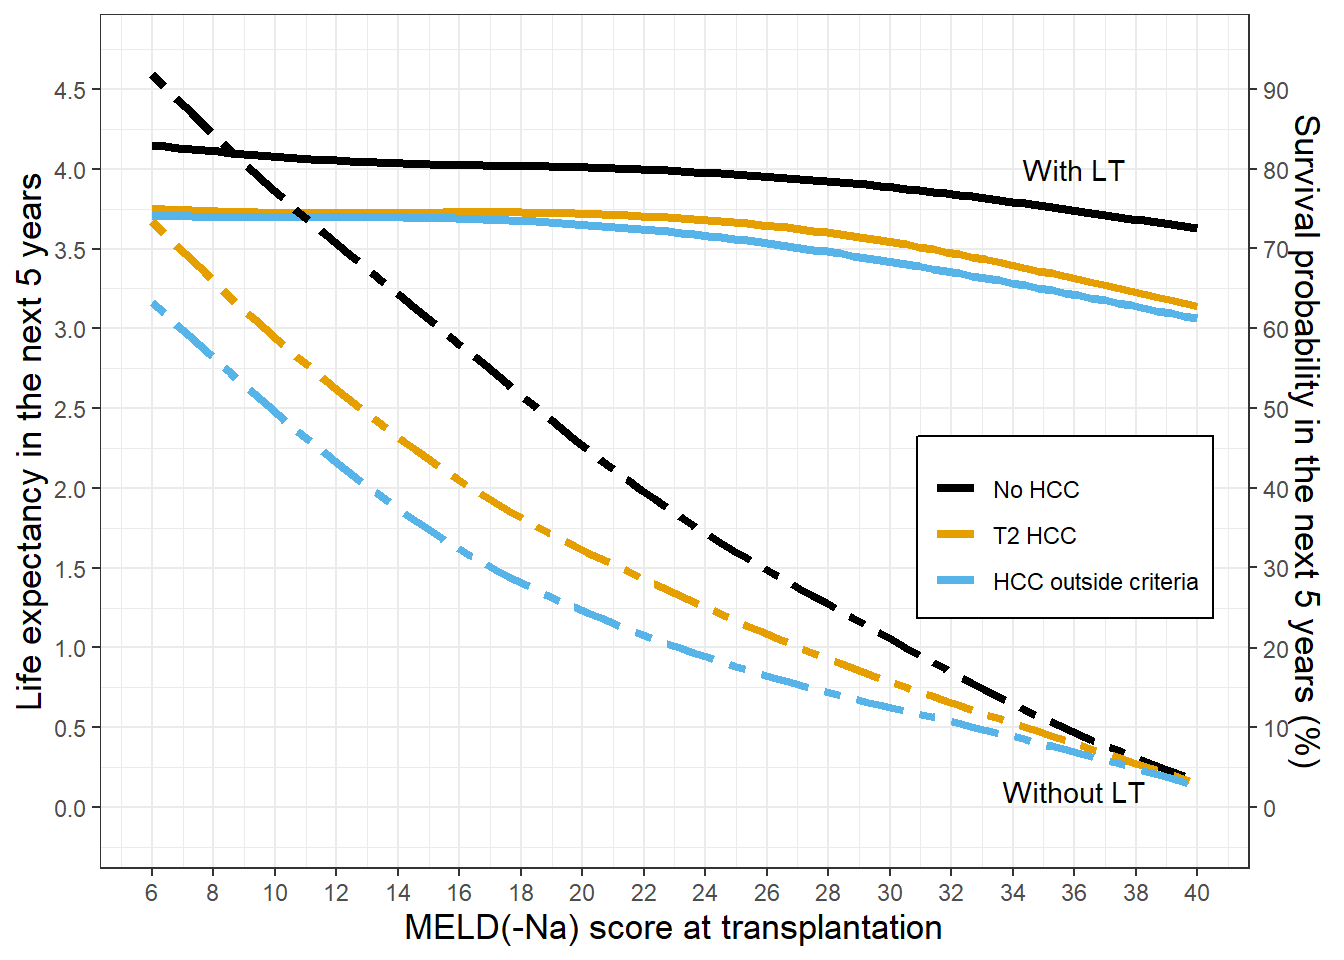
\includegraphics{thesis_files/figure-latex/benefit-fig3a-1} }\newline\subfloat[The survival benefit of liver transplantation per MELD(-Na) score, which is the difference between the dashed and solid lines in A.\label{fig:benefit-fig3a-2}]{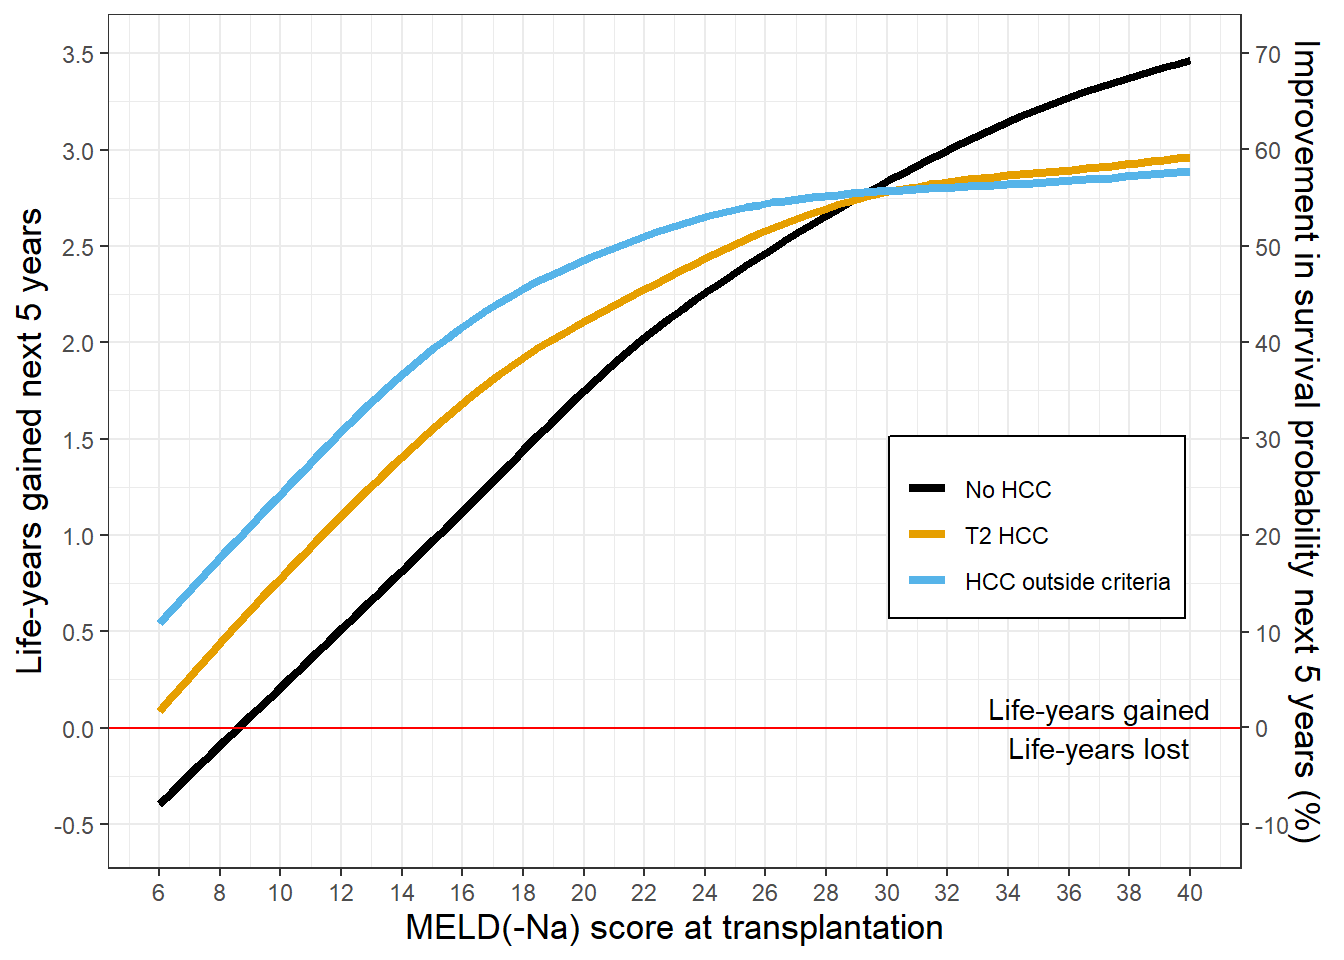
\includegraphics{thesis_files/figure-latex/benefit-fig3a-2} }\caption{The mean survival and benefit for the next five years per MELD(-Na) score. Note the changing y-axes.}\label{fig:benefit-fig3a}
\end{figure}

\hypertarget{survival-benefit-life-years-gained-per-5-years}{%
\subsection*{Survival benefit: life-years gained per 5 years}\label{survival-benefit-life-years-gained-per-5-years}}
\addcontentsline{toc}{subsection}{Survival benefit: life-years gained per 5 years}

The 5-year transplantation survival benefit per MELD(-Na) score and per (non-)HCC disease is shown in Figure \ref{fig:benefit-fig3a}B and Table \ref{tab:benefit-tab2} (see Table S4 for the averages per MELD(-Na) score). Please note that the y-values correspond to the surface area shown in Figure \ref{fig:benefit-fig1b}, e.g., for a non-HCC MELD(-Na) 25 patient, LT would give 2.35 years survival benefit during the next five years.

For the 2.2\% of non-HCC patients transplanted at MELD(-Na) below 9, benefit was negative, because mean postoperative life-expectancy was lower than survival without LT. With increasing MELD(-Na) scores, non-HCC benefit increased approximately linearly, up to 70\% mean 5-year survival improvement for MELD(-Na) 40. The HCC benefit curves flattened with increasing MELD(-Na), whereas non-HCC benefit continued to increase. HCC MELD(-Na) \textgreater=30 benefit estimates should be interpreted carefully as they represent a small number of patients, i.e., 4.5\% of the T2 HCC and 2.8\% of the outside criteria HCC patients. The HCC benefit flattened at higher MELD(-Na) scores because of decreasing post-transplant survival, see Figure \ref{fig:benefit-fig3a}A.
Below MELD(-Na) 30, HCC patients would gain more benefit than non-HCC patients at the same MELD(-Na) score, which was mainly due to the lower expected HCC waiting list survival in absence of LT. However, the likelihood of transplantation at lower MELD(-Na) was much lower for non-HCC patients. Figure \ref{fig:benefit-fig2} and Table \ref{tab:benefit-tab2} show that most non-HCC patients were transplanted at higher benefit scores than most HCC patients. Indeed, over 50\% of HCC patients were transplanted below MELD(-Na) 14, whereas over 50\% of non-HCC patients were transplanted above MELD(-Na) 26. In terms of benefit, most HCC patients gained 0.10 to 1.96 years from LT, whereas most non-HCC patients gained 2.48 to 3.46 years (Table S4). For all patients across all MELD(-Na) scores, non-HCC patients gained 3.2 years in the next 5 years through transplantation, T2 HCC gained 1.19 and HCC outside criteria gained 1.45 life-years, see Table \ref{tab:benefit-tab2}.

\linespread{1}

\begin{table}

\caption{\label{tab:benefit-tab2}Liver transplantation 5-year survival benefit per MELD(-Na) score and etiology of disease}
\centering
\resizebox{\linewidth}{!}{
\begin{threeparttable}
\begin{tabular}[t]{lrllrllrll}
\toprule
\multicolumn{1}{c}{ } & \multicolumn{3}{c}{No HCC} & \multicolumn{3}{c}{T2 HCC} & \multicolumn{3}{c}{HCC outside criteria} \\
\cmidrule(l{3pt}r{3pt}){2-4} \cmidrule(l{3pt}r{3pt}){5-7} \cmidrule(l{3pt}r{3pt}){8-10}
MELD(-Na) & n & \% & benefit & n & \% & benefit & n & \% & benefit\\
\midrule
\cellcolor{gray!6}{6-9} & \cellcolor{gray!6}{175} & \cellcolor{gray!6}{2.2} & \cellcolor{gray!6}{-0.14} & \cellcolor{gray!6}{729} & \cellcolor{gray!6}{32.0} & \cellcolor{gray!6}{0.39} & \cellcolor{gray!6}{717} & \cellcolor{gray!6}{39.2} & \cellcolor{gray!6}{0.82}\\
10-13 & 425 & 5.3 & 0.46 & 675 & 29.6 & 0.98 & 525 & 28.7 & 1.40\\
\cellcolor{gray!6}{14-17} & \cellcolor{gray!6}{943} & \cellcolor{gray!6}{11.7} & \cellcolor{gray!6}{1.08} & \cellcolor{gray!6}{416} & \cellcolor{gray!6}{18.2} & \cellcolor{gray!6}{1.61} & \cellcolor{gray!6}{304} & \cellcolor{gray!6}{16.6} & \cellcolor{gray!6}{2.03}\\
18-21 & 1134 & 14.1 & 1.67 & 197 & 8.6 & 2.02 & 153 & 8.4 & 2.37\\
\cellcolor{gray!6}{22-25} & \cellcolor{gray!6}{1260} & \cellcolor{gray!6}{15.6} & \cellcolor{gray!6}{2.20} & \cellcolor{gray!6}{106} & \cellcolor{gray!6}{4.6} & \cellcolor{gray!6}{2.37} & \cellcolor{gray!6}{59} & \cellcolor{gray!6}{3.2} & \cellcolor{gray!6}{2.65}\\
26-29 & 1064 & 13.2 & 2.60 & 56 & 2.5 & 2.69 & 17 & 0.9 & 2.72\\
\cellcolor{gray!6}{30-34} & \cellcolor{gray!6}{1159} & \cellcolor{gray!6}{14.4} & \cellcolor{gray!6}{2.99} & \cellcolor{gray!6}{41} & \cellcolor{gray!6}{1.8} & \cellcolor{gray!6}{2.78} & \cellcolor{gray!6}{21} & \cellcolor{gray!6}{1.1} & \cellcolor{gray!6}{2.72}\\
35-40 & 1900 & 23.6 & 3.38 & 61 & 2.7 & 2.92 & 31 & 1.7 & 2.85\\
\textcolor{black}{\textbf{\cellcolor{gray!6}{All patients}}} & \textcolor{black}{\textbf{\cellcolor{gray!6}{8060}}} & \textcolor{black}{\textbf{\cellcolor{gray!6}{100}}} & \textcolor{black}{\textbf{\cellcolor{gray!6}{2.30}}} & \textcolor{black}{\textbf{\cellcolor{gray!6}{2281}}} & \textcolor{black}{\textbf{\cellcolor{gray!6}{100}}} & \textcolor{black}{\textbf{\cellcolor{gray!6}{1.19}}} & \textcolor{black}{\textbf{\cellcolor{gray!6}{1827}}} & \textcolor{black}{\textbf{\cellcolor{gray!6}{100}}} & \textcolor{black}{\textbf{\cellcolor{gray!6}{1.45}}}\\
\bottomrule
\end{tabular}
\begin{tablenotes}
\item \textit{Note: } 
\item n: number of patients per MELD(-Na) group, \% : percentage of patients per MELD(-Na) group
\end{tablenotes}
\end{threeparttable}}
\end{table}

\linespread{1.213}

\hypertarget{liver-transplant-benefit-scores}{%
\subsection*{Liver transplant benefit scores}\label{liver-transplant-benefit-scores}}
\addcontentsline{toc}{subsection}{Liver transplant benefit scores}

Liver transplant benefit scores could be used as a continuous, equalizing metric for (non-)HCC LT access. There might be a need to calculate benefit given specific patient characteristics. This is now possible in the online benefit calculator: \url{https://predictionmodels.shinyapps.io/benefit_calculator/}. The calculator was based on a secondary regression analysis with only the most important benefit predictors, which showed an optimism corrected R\textsuperscript{2} of 0.93. We therefore assumed that the calculator adequately predicted benefit and could serve as translation from our complex analyses to clinical practice. Variable importance in regression was summarized in Figure S4. When predicting benefit, the MELD(-Na) score was by far most important. Next were serum albumin, (non-)HCC disease, serum sodium levels, and recipient age. In line with Schaubel et al.,\textsuperscript{21} liver function therefore remained the strongest predictor of survival benefit.
Lastly, the online app also allows users to plot mean benefit per MELD-Na and (non-)HCC disease, like Figure \ref{fig:benefit-fig1a}. This can be used to inform clinicians and patients on the expected survival gain from transplantation. It also shows for selected HCC patients which non-HCC patients have equal benefit, i.e., which patients would compete for transplant based on benefit scores.

\hypertarget{discussion-4}{%
\section*{Discussion}\label{discussion-4}}
\addcontentsline{toc}{section}{Discussion}

Organ allocation aims to equally distribute donor organs to all patients in need. However, inequities on the LT waiting list exist. As a result, liver allocation has become increasingly relevant and complex. Survival benefit has gained increased attention,\textsuperscript{13,14,16,17,29} as its optimization could improve life-years gained from transplantation for all listed patients.\textsuperscript{21} Also, considering survival with and without LT based on patient characteristics closer resembles clinical reasoning.
The objective of this study was to estimate and compare LT survival benefit for patients with and without HCC in a recent US waiting list cohort. The novelty was estimating benefit from the moment of transplantation based on longitudinal disease development up until that moment. Our results showed that mean LT survival benefit was positive across all MELD(-Na) scores, except for non-HCC patients with MELD(-Na) scores below 9. Non-HCC patients gained most life years from transplantation, as these patients were mostly transplanted above MELD(-Na) 26, where benefit was highest. HCC patients were mostly transplanted below MELD(-Na) 14, which yielded lower survival benefit. Liver function was the most important predictor of benefit. It is now possible online to calculate 5-year survival benefit based on specific patient characteristics through \url{https://predictionmodels.shinyapps.io/benefit_calculator/}.

\hypertarget{benefit-definition-1}{%
\subsection*{Benefit definition}\label{benefit-definition-1}}
\addcontentsline{toc}{subsection}{Benefit definition}

Benefit was defined as the difference in survival with and without LT during the next five years. The endpoint of survival analysis was five years, because using 10-year or overall survival as outcome would give too much importance to variables that predict post-transplant survival.\textsuperscript{4,29} Also, further increasing the prediction horizon made estimates less certain. At five years, the waiting list model showed an excellent AUC, also when compared to other similar analyses.\textsuperscript{21,23} Compared to recently reported and tested post-transplant survival models, our 5-year post-transplant survival model performed similar (LiTES) or better (HALT-HCC, Metroticket).\textsuperscript{10}

\hypertarget{estimation-of-benefit}{%
\subsection*{Estimation of benefit}\label{estimation-of-benefit}}
\addcontentsline{toc}{subsection}{Estimation of benefit}

We choose our methods to estimate benefit from the moment of possible LT. These methods differed from previous clinical studies that modeled waiting list survival counted from first registration.\textsuperscript{13,16,17,32,36} Our goal was to model future survival without LT, whereas counting from baseline gives survival before LT, see Figure \ref{fig:benefit-fig1a}. Also, patient states at first listing and transplantation should not be compared, as survival changes within each patient over waiting list time due to e.g., disease progression and possible non-LT treatments.\textsuperscript{6,21,22,24--26} We therefore calculated counterfactual waiting list survival (without LT) through time-dependent analysis with additional correction for bias.\textsuperscript{21,26} Others performed similar analyses over time, but averaged calculated benefit over waiting list follow-up,\textsuperscript{21,23} which for us seemed suboptimal as possible transplantation and its benefit occurred at one moment in time per patient. Lastly, some previous studies calculated benefit using characteristics of a `median donor' assigned to all patients.\textsuperscript{13,37} Instead, we choose to use the actual transplantations between 2010-2019, with the aim to best evaluate reality, as the observed transplants indicate inequity between (non-)HCC patients.\textsuperscript{5}

\hypertarget{non-hcc-and-hcc-benefit}{%
\subsection*{Non-HCC and HCC benefit}\label{non-hcc-and-hcc-benefit}}
\addcontentsline{toc}{subsection}{Non-HCC and HCC benefit}

A competing risks study by Berry et al.~showed that HCC patients in the US overall gained negative or little benefit from transplantation, i.e., that HCC patients wasted benefit.\textsuperscript{13} This contrasts with our findings that mean HCC benefit was positive across all MELD(-Na) scores, mainly because HCC survival without LT was low. Clinically, it makes sense that out of two otherwise identical patients, the patient with HCC will live shorter without LT because of the malignancy in situ.\textsuperscript{38} It was suggested that Berry et al.~overestimated HCC waiting list survival,\textsuperscript{39} and that having HCC increased risk of waiting list mortality by factor 1.5.\textsuperscript{21}

Therefore, on the individual patient level, transplantation for HCC will add life years. However, on a population level, (over)prioritizing HCC patients can indirectly waste benefit, as non-HCC patients often will gain more survival from LT due to worse liver function. Interestingly, many HCC patients were transplanted at MELD(-Na) \textless10, which was considered harmful in previous study.\textsuperscript{36} Moreover, resectable HCC may be regarded a contra-indication for LT,\textsuperscript{4} especially when considering the limited number of available liver donors. Therefore, the selection of HCC patients for transplantation remains one of the most important parts of liver graft allocation.\textsuperscript{29}

\hypertarget{using-benefit-scores}{%
\subsection*{Using benefit scores}\label{using-benefit-scores}}
\addcontentsline{toc}{subsection}{Using benefit scores}

The LT benefit scores offer a continuous metric to stratify survival equally for non-HCC and HCC patients, as one single model is used for both groups. This abandons the use of waiting time, which is inherently flawed,\textsuperscript{19} and binary criteria, which allow underreporting of HCC severity.\textsuperscript{40,41} Current HCC criteria lack granularity, as patients that have the same waiting list priority can have very different survival with(out) LT.\textsuperscript{10,13,17,21} Changing LT priority based on benefit scores could therefore prevent loss of life-years, as also shown in simulations.\textsuperscript{21} Allocation policies like the HCC cap, HCC delay, and Median MELD at Transplant helped to reduce HCC LT access, but HCC patients are currently still better of regarding waiting time, transplantation rates, and death rates.\textsuperscript{5,42} Clearly, there is a need for an equalizing principle for all eligible LT candidates.

Still, consensus must be reached whether to consider benefit in allocation at all. Understandably, some feel uncomfortable to base treatment decisions on future posttransplant outcomes, which is in part why US policy first focused on improving regional disparities.\textsuperscript{15,43,44} On the other hand, there is consensus on acceptable posttransplant outcomes,\textsuperscript{45} and posttransplant survival can be accurately predicted. Interestingly, in the UK, a benefit-based allocation system was implemented in 2018.\textsuperscript{46} The evaluation of this system will be valuable for the debate on benefit and its role in liver allocation. However, it is most important that, regardless of the driving allocation principle, scarce liver grafts should be fairly distributed based on patient characteristics and disease severity, not arbitrary exception points.

\hypertarget{limitations-4}{%
\subsection*{Limitations}\label{limitations-4}}
\addcontentsline{toc}{subsection}{Limitations}

Our study has limitations. We excluded a minority of patients with exception points that did not have HCC, our findings might therefore not apply to the whole waiting list population. However, our goal was to compare non-HCC and HCC patients. Also, five-year post-transplant follow-up was not complete for all patients, as we compromised completeness and study period. Furthermore, we could only draw conclusions based on patients that were listed for transplantation. Therefore, selection bias exists, which is inherent to the analysis of registries. The UNOS also does not register HCC recurrence, which would be valuable as HCC recurrence rates can be up to 20\%, after which median survival is less than a year.\textsuperscript{41} Studying these data in HCC MELD\textgreater30 patients would be especially interesting. Still, overall mortality is considered free from bias, whereas disease-specific survival is not.\textsuperscript{47} Also, due to the small number of transplantations in HCC patients with MELD(-Na)\textgreater30, estimates were less reliable for that group. Lastly, the presented time-dependent IPC-weighted analyses are complex and not intuitively interpreted. However, this complexity was needed to calculate future survival without LT and to best answer the clinical question of survival benefit. We attempted to translate complexity into an easy-accessible online benefit calculator.

\hypertarget{conclusion-4}{%
\section*{Conclusion}\label{conclusion-4}}
\addcontentsline{toc}{section}{Conclusion}

In conclusion, on an individual level, transplanting patients with HCC resulted in survival benefit. However, on a population level, benefit was indirectly wasted, as non-HCC patients were likely to gain more survival due to decreased liver function. Liver transplant benefit scores offer equal survival stratification for (non-)HCC patients. It is now possible online to calculate these scores based on individual patient characteristics. Considering benefit better resembles clinical reasoning and can optimize life years gained for the whole waiting list population. Survival benefit scores could therefore serve to more equally allocate scarce liver grafts amongst patients eligible for transplantation.

\newpage
\linespread{1}
\small

\hypertarget{references-5}{%
\section*{References}\label{references-5}}
\addcontentsline{toc}{section}{References}

\begin{enumerate}
\def\labelenumi{\arabic{enumi}.}
\tightlist
\item
  Tschuor C, Ferrarese A, Kuemmerli C, et al.~Allocation of liver grafts worldwide -- Is there a best system? J Hepatol. 2019;71(4):707-718. \url{doi:10.1016/j.jhep.2019.05.025}
\item
  Kim WR, Biggins SW, Kremers WK, et al.~Hyponatremia and Mortality among Patients on the Liver-Transplant Waiting List. N Engl J Med. 2008;359(10):1018-1026. \url{doi:10.1007/s11250-017-1262-3}
\item
  Goudsmit BFJ, Putter H, Tushuizen ME, et al.~Validation of the Model for End‐stage Liver Disease sodium (MELD‐Na) score in the Eurotransplant region. Am J Transplant. Published online 2020. \url{doi:10.1111/ajt.16142}
\item
  Vitale A, Cucchetti A, Qiao GL, et al.~Is resectable hepatocellular carcinoma a contraindication to liver transplantation? A novel decision model based on ``number of patients needed to transplant'' as measure of transplant benefit. J Hepatol. 2014;60(6):1165-1171. \url{doi:10.1016/j.jhep.2014.01.022}
\item
  Kwong AJ, Kim WR, Lake JR, et al.~OPTN/SRTR 2019 Annual Data Report: Liver. Am J Transplant. 2021;21(S2):208-315. \url{doi:10.1111/ajt.16494}
\item
  Mazzaferro V, Citterio D, Bhoori S, et al.~Liver transplantation in hepatocellular carcinoma after tumour downstaging ( XXL ): a randomised , controlled ,. Lancet Oncol. 2020;21(7):947-956. \url{doi:10.1016/S1470-2045(20)30224-2}
\item
  Global Burden of Disease Cancer Collaboration, Fitzmaurice C, Allen C, et al.~Global, Regional, and National Cancer Incidence, Mortality, Years of Life Lost, Years Lived With Disability, and Disability-Adjusted Life-years for 32 Cancer Groups, 1990 to 2015: A Systematic Analysis for the Global Burden of Disease Study. JAMA Oncol. 2016;388(10053):1459-1544. \url{doi:10.1001/jamaoncol.2016.5688}
\item
  Galle PR, Forner A, Llovet JM, et al.~Clinical Practice Guidelines OF HEPATOLOGY EASL Clinical Practice Guidelines: Management of hepatocellular carcinoma q. J Hepatol. 2018;69(1):182-236. \url{doi:10.1016/j.jhep.2018.03.019}
\item
  Alver SK, Lorenz DJ, Marvin MR, Brock GN. Projected outcomes of 6-month delay in exception points versus an equivalent Model for End-Stage Liver Disease score for hepatocellular carcinoma liver transplant candidates. Liver Transplant. 2016;22(10):1343-1355. \url{doi:10.1002/lt.24503}
\item
  Goldberg D, Mantero A, Newcomb C, et al.~Predicting survival after liver transplantation in patients with hepatocellular carcinoma using the LiTES-HCC score. J Hepatol. Published online 2021:1-9. \url{doi:10.1016/j.jhep.2020.12.021}
\item
  Freeman RB, Gish RG, Harper A, et al.~Model for End-Stage Liver Disease (MELD) Exception Guidelines: Results and Recommendations From the MELD Exception Study Group and Conference (MESSAGE) for the Approval of Patients Who Need Liver Transplantation With Diseases Not Considered by the Standar. Liver Transplant. 2007;13(5):767-768. \url{doi:10.1002/lt}
\item
  Northup PG, Intagliata NM, Shah NL, Pelletier SJ, Berg CL, Argo CK. Excess mortality on the liver transplant waiting list: Unintended policy consequences and model for End-Stage Liver Disease (MELD) inflation. Hepatology. 2015;61(1):285-291. \url{doi:10.1002/hep.27283}
\item
  Berry K, Ioannou GN. Comparison of Liver Transplant-Related Survival Benefit in Patients with Versus Without Hepatocellular Carcinoma in the United States. Gastroenterology. 2015;149(3):669-680. \url{doi:10.1053/j.gastro.2015.05.025}
\item
  Washburn K, Edwards E, Harper A, Freeman RB. Hepatocellular Carcinoma Patients Are Advantaged in the Current Liver Transplant Allocation System. Am J Transplant. 2010;10(7):1652-1657. \url{doi:10.1111/j.1600-6143.2010.03127.x}
\item
  OPTN/UNOS Liver and Intestinal Transplantation Committee. OPTN / UNOS Policy Notice Revisions to National Liver Review Board Policies. Published 2019. Accessed April 21, 2021. \url{https://optn.transplant.hrsa.gov/media/2816/liver_nlrb-revised-policynotice-dsa_01252019.pdf}
\item
  Toso C, Dupuis-Lozeron E, Majno P, et al.~A model for dropout assessment of candidates with or without hepatocellular carcinoma on a common liver transplant waiting list. Hepatology. 2012;56(1):149-156. \url{doi:10.1002/hep.25603}
\item
  Vitale A, Volk ML, De Feo TM, et al.~A method for establishing allocation equity among patients with and without hepatocellular carcinoma on a common liver transplant waiting list. J Hepatol. 2014;60(2):290-297. \url{doi:10.1016/j.jhep.2013.10.010}
\item
  Mehta N, Dodge JL, Roberts JP, Yao FY. A novel waitlist dropout score for hepatocellular carcinoma - identifying a threshold that predicts worse post-transplant survival. J Hepatol. Published online 2020:1-9. \url{doi:10.1016/j.jhep.2020.10.033}
\item
  Persad G, Wertheimer A, Emanuel EJ. Principles for allocation of scarce medical interventions. Lancet. 2009;373(9661):423-431. \url{doi:10.1016/S0140-6736(09)60137-9}
\item
  Merion RM, Schaubel DE, Dykstra DM, Freeman RB, Port FK, Wolfe RA. The survival benefit of liver transplantation. Am J Transplant. 2005;5(2):307-313. \url{doi:10.1111/j.1600-6143.2004.00703.x}
\item
  Schaubel DE, Guidinger MK, Biggins SW, et al.~Survival benefit-based deceased-donor liver allocation. Am J Transplant. 2009;9(4 PART 2):970-981. \url{doi:10.1111/j.1600-6143.2009.02571.x}
\item
  Schaubel DE, Sima CS, Goodrich NP, Feng S, Merion RM. The survival benefit of deceased donor liver transplantation as a function of candidate disease severity and donor quality. Am J Transplant. 2008;8(2):419-425. \url{doi:10.1111/j.1600-6143.2007.02086.x}
\item
  Sharma P, Schaubel DE, Goodrich NP, Merion RM. Serum Sodium and Survival Benefit of Liver Transplantation. Liver Transplant. 2015;21:308-313. \url{doi:10.1002/lt}.
\item
  Merion RM, Wolfe RA, Dykstra DM, Leichtman AB, Gillespie B, Held PJ. Longitudinal assessment of mortality risk among candidates for liver transplantation. Liver Transplant. 2003;9(1):12-18. \url{doi:10.1053/jlts.2003.50009}
\item
  Goudsmit BFJ, Braat AE, Tushuizen ME, et al.~Joint modeling of liver transplant candidates outperforms the model for end-stage liver disease: The effect of disease development over time on patient outcome. Am J Transplant. 2021;(June):ajt.16730. \url{doi:10.1111/ajt.16730}
\item
  Gong Q, Schaubel DE. Estimating the average treatment effect on survival based on observational data and using partly conditional modeling. Biometrics. 2017;73(1):134-144. \url{doi:10.1111/biom.12542}
\item
  Mazzaferro V, REGALIA E, DOCI R, et al.~Liver transplantation for the treatment of small hepatocellular carcinomas in patients with cirrhosis. N Engl J Med. 1996;334(11):693-699.
\item
  Yao FY, Kerlan RK, Hirose R, et al.~Excellent outcome following down-staging of hepatocellular carcinoma prior to liver transplantation: An intention-to-treat analysis. Hepatology. 2008;48(3):819-827. \url{doi:10.1002/hep.22412}
\item
  Cillo U, Vitale A, Polacco M, Fasolo E. Liver transplantation for hepatocellular carcinoma through the lens of transplant benefit. Hepatology. 2017;65(5):1741-1748. \url{doi:10.1002/hep.28998}
\item
  van Geloven N, Swanson SA, Ramspek CL, et al.~Prediction meets causal inference: the role of treatment in clinical prediction models. Eur J Epidemiol. 2020;35(7):619-630. \url{doi:10.1007/s10654-020-00636-1}
\item
  Llovet JM, Fuster J, Bruix J. Intention-to-treat analysis of surgical treatment for early hepatocellular carcinoma: Resection versus transplantation. Hepatology. 1999;30(6):1434-1440. \url{doi:10.1002/hep.510300629}
\item
  Lai Q, Vitale A, Iesari S, et al.~Intention-to-treat survival benefit of liver transplantation in patients with hepatocellular cancer. Hepatology. 2017;66(6):1910-1919. \url{doi:10.1002/hep.29342}
\item
  Kaplan A. The Conduct of Inquiry: Methodology for Behavioral Science. Chandler; Chandler; 1964.
\item
  Harrell FE. Regression Modeling Strategies. Vol 45.; 2003. \url{doi:10.1198/tech.2003.s158}
\item
  Van Calster B, McLernon DJ, Van Smeden M, et al.~Calibration: The Achilles heel of predictive analytics. BMC Med. 2019;17(1):1-7. \url{doi:10.1186/s12916-019-1466-7}
\item
  Vitale A, Huo T La, Cucchetti A, et al.~Survival Benefit of Liver Transplantation Versus Resection for Hepatocellular Carcinoma: Impact of MELD Score. Ann Surg Oncol. 2015;22(6):1901-1907. \url{doi:10.1245/s10434-014-4099-2}
\item
  Luo X, Leanza J, Massie AB, et al.~MELD as a metric for survival benefit of liver transplantation. Am J Transplant. 2018;18(5):1231-1237. \url{doi:10.1111/ajt.14660}
\item
  Vitale A, Volk ML, Senzolo M, Frigo AC, Cillo U. Estimation of Liver Transplant Related Survival Benefit: The Devil Is in the Details. Gastroenterology. 2016;150(2):534-535. \url{doi:10.1053/j.gastro.2015.12.002}
\item
  Mehta N, Heimbach J, Hirose R, Roberts JP, Yao FY. Minimal Transplant Survival Benefit for Hepatocellular Carcinoma: Is it Real or an Overestimation of Waitlist Life Expectancy? Gastroenterology. 2016;150(2):533-534. \url{doi:10.1053/j.gastro.2015.08.059}
\item
  Aufhauser DD, Sadot E, Murken DR, et al.~Incidence of Occult Intrahepatic Metastasis in Hepatocellular Carcinoma Treated with Transplantation Corresponds to Early Recurrence Rates after Partial Hepatectomy. Ann Surg. 2018;267(5):922-928. \url{doi:10.1097/SLA.0000000000002135}
\item
  Mahmud N, Hoteit MA, Goldberg DS. Risk Factors and Center-Level Variation in Hepatocellular Carcinoma Under-Staging for Liver Transplantation. Liver Transplant. 2020;26(8):977-988. \url{doi:10.1002/lt.25787}
\item
  Northup PG, Intagliata NM, Shah NL, Pelletier SJ, Berg CL, Argo CK. Excess mortality on the liver transplant waiting list: Unintended policy consequences and model for End-Stage Liver Disease (MELD) inflation. Hepatology. 2015;61(1):285-291. \url{doi:10.1002/hep.27283}
\item
  Kadry Z, Schaefer EW, Uemura T, Shah AR, Schreibman I, Riley TR. Impact of geographic disparity on liver allocation for hepatocellular cancer in the United States. J Hepatol. 2012;56(3):618-625. \url{doi:10.1016/j.jhep.2011.08.019}
\item
  Neuberger J, Heimbach JK. Allocation of deceased-donor livers -- Is there a most appropriate method? J Hepatol. 2019;71(4):654-656. \url{doi:10.1016/j.jhep.2019.07.013}
\item
  Mehta N, Bhangui P, Yao FY, et al.~Liver Transplantation for Hepatocellular Carcinoma. Working Group Report from the ILTS Transplant Oncology Consensus Conference. Transplantation. 2020;104(6):1136-1142. \url{doi:10.1097/TP.0000000000003174}
\item
  National Health Service Blood and Transplantat. Policy for Deceased Donor Liver Distribution and Allocation. Published online 2018:1-18. \url{http://www.odt.nhs.uk/transplantation/tools-policies-and-guidance/policies-and-guidance/}
\end{enumerate}

\newpage
\linespread{1.213}
\normalsize
\thispagestyle{plain}

\mbox{}

\addtocontents{toc}{\setcounter{tocdepth}{0}}
\pagecolor{black}
\color{white}

\hypertarget{part-iv-summary-general-discussion-and-future-perspectives}{%
\chapter*{Part IV: Summary, general discussion, and future perspectives}\label{part-iv-summary-general-discussion-and-future-perspectives}}
\addcontentsline{toc}{chapter}{Part IV: Summary, general discussion, and future perspectives}

\chaptermark{Forms of MELD}

\chaptermark{summary, discussion, perspectives}

\begin{quote}
\emph{``Zodat het dan net lijkt alsof u vanaf het begin al de meest verantwoorde gedachten had over uw variabelen (u weet wel, die dingen waar u achteraf altijd zo'n spijt van had), en over uw hypothesen (u weet wel, die dingen die u dan achteraf verzon om het nog ergens op te laten lijken).''}
\end{quote}

\begin{quote}
--- Arno Goudsmit
\end{quote}

\begin{center}\rule{0.5\linewidth}{0.5pt}\end{center}

\newpage

\hypertarget{summ}{%
\chapter{Summary}\label{summ}}

\newpage
\nopagecolor
\color{black}

The persistent scarcity of donor liver grafts necessitates prioritization of patients based on expected future survival without transplantation. The goal of this thesis was to improve survival prediction models for patients on the LT waiting list. Through advancements in prediction models, liver grafts can be allocated in the best way possible.

In \textbf{Chapter \ref{chap-meldna}}, the MELD-Na score (devised in the UNOS region) was validated for the Eurotransplant region. We investigated the relationship between serum sodium levels, MELD scores, and 90-day mortality. Hyponatremia of \textless135, \textless130, and \textless125 mmol/L was found in respectively 28.5\%, 8.8\%, and 2.6\% of the patients. We found that between 140 and 125 mmol/L, the risk of 90-day death increased threefold (HR 2.9; 95\% CI 2.30-3.53; p\textless0.001). Every point decrease in serum sodium levels increased 90-day mortality by 8\% (HR 0.92; 95\% CI 0.90-0.94; p\textless0.001). Concordance statistics of MELD and MELD-Na were 0.832 and 0.847, respectively. Predictions based on MELD-Na were also more accurate than MELD. Comparing the possible impact of using MELD-Na instead of MELD for allocation on the waiting list, we found that approximately 20\% of patients would receive a significantly higher predicted risk of death with MELD-Na and therefore a better chance for timely LT.

In \textbf{Chapter \ref{chap-refit}}, the 20-year-old UNOS MELD score was refitted to the Eurotransplant population. We assessed the relation of each MELD(-Na) parameter to 90-day mortality. Based on the data, the lower and upper parameter bounds and coefficients with the best fit were established. Specifically: creatinine 0.7- 2.5 mg/dL, bilirubin 0.3- 27 mg/dL, INR 0.1- 2.6, and sodium 120- 139 mmol/L. The resulting reMELD(-Na) significantly improved fit, discrimination, and calibration compared to MELD(-Na). Compared to MELD, reMELD-Na could have prioritized patients with on average 1.6 times higher 90-day mortality, thus better effectuating the sickest-first principle.

In \textbf{Chapter \ref{chap-jm}}, we developed and validated joint models for the Eurotransplant (MELD-JM) and UNOS (MELDNa-JM) regions. Repeated MELD(-Na) measurements were modeled flexibly over time and joined with Cox proportional hazards models. It was found that both MELD(-Na) value and its rate of change were strongly associated with waiting list mortality. The JMs significantly improved AUCs and Brier scores for waiting list survival prediction in both regions. MELD(Na)-JM possibly could have prioritized patients with three to five times higher 90-day waiting list mortality than MELD(-Na).

In \textbf{Chapter \ref{chap-aclfjm}}, we constructed and validated the ACLF-JM for patients with ACLF on the waiting list. For the ACLF-JM, repeated MELD-Na scores were corrected for CLIF-C OF scores at baseline, age, sex, life-support dependency, presence of bacterial peritonitis, and presence of cirrhosis. ACLF-JM performance was compared to a landmark MELD-Na Cox model. ACLF grade 1 to 3 was present in respectively 16.4\%, 10.4\%, and 6.2\% of the patients. ACLF-JM performance, measured through AUCs and prediction errors, was significantly better than landmark MELD-Na. The ACLF-JM identified patients with lower MELD-Na scores but four times higher 90-day mortality.

In \textbf{Chapter \ref{chap-benefit}}, we studied the survival benefit that LT caused, by comparing 5-year survival with and without LT between patients with and without HCC in the US. HCC patients had lower waiting list survival than non-HCC patients. Most HCC patients were transplanted below MELD(-Na) 14 and most non-HCC patients above MELD(-Na) 26. Liver function (MELD(-Na), albumin) was the main predictor of 5-year benefit. Therefore, during five years, most HCC patients gained 0.12 to 1.96 years from LT, whereas most non-HCC patients gained 2.48 to 3.45 years. Thus, on an individual level, transplanting patients with HCC resulted in survival benefit. However, on a population level, benefit was indirectly wasted, as non-HCC patients were likely to gain more survival due to decreased liver function.

\newpage
\pagecolor{black}
\color{white}
\thispagestyle{plain}

\mbox{}

\hypertarget{gendisc}{%
\chapter{General discussion}\label{gendisc}}

\newpage
\nopagecolor
\color{black}

\hypertarget{part-i-forms-of-meld-1}{%
\subsection*{Part I: Forms of MELD}\label{part-i-forms-of-meld-1}}
\addcontentsline{toc}{subsection}{Part I: Forms of MELD}

In \textbf{Chapter \ref{chap-meldna}}, we showed that hyponatremia increased 90-day waiting list mortality. We also found that MELD-Na was a significantly better predictor of waiting list survival than MELD. Prioritization based on MELD-Na survival predictions could therefore reduce waiting list mortality. However, in the Eurotransplant region, MELD-Na is still not used for liver allocation.

\hypertarget{sodium-levels-and-post-transplant-survival}{%
\subsubsection*{Sodium levels and post-transplant survival}\label{sodium-levels-and-post-transplant-survival}}
\addcontentsline{toc}{subsubsection}{Sodium levels and post-transplant survival}

One of the concerns in the Eurotransplant community was that prioritizing hyponatremic patients for LT could decrease post-transplant survival. This concern arose in part because pre-transplant sodium levels are associated with increased morbidity, complications, and hospital admission.\textsuperscript{1} Some older European studies indeed showed decreased short-term post-transplant survival in hyponatremic LT recipients.\textsuperscript{2,3} Still, in recent Eurotransplant data, we found no significant post-transplant survival differences between normo- and hyponatremic LT recipients (data not published). This is in agreement with the largest study on post-transplant sodium effects in the US.\textsuperscript{4} MELD-Na evaluation also showed that after implementing the score for allocation, the negative effect of hyponatremia on waiting list mortality was greatly reduced.\textsuperscript{5}

In the US, MELD-Na was implemented for MELD\textgreater11 patients after studying the effect of serum sodium levels on both survival with and without LT.\textsuperscript{6} Ideally, such analyses would also have been done in Eurotransplant. However, the required longitudinal sodium data is not available, as sodium is not adequately registered. In our validation study, we had to exclude two-thirds of eligible patients at baseline due to missing sodium. This missingness forms the most important limitation and rationale of our MELD-Na validation study. MELD-Na implementation could further improve waiting list ranking than found in this study because missing data analysis suggested that hyponatremia likely was more prevalent in patients with missing sodium data, as these patients significantly more often had alcohol-induced cirrhosis and higher creatinine levels. The seminal validation study of MELD by Wiesner et al.~also excluded 48\% (n=3,214) of patients due to missing data.\textsuperscript{7} This illustrates that sometimes evidence of improvement is provided despite missing data.

\hypertarget{sodium-levels-and-renal-function}{%
\subsubsection*{Sodium levels and renal function}\label{sodium-levels-and-renal-function}}
\addcontentsline{toc}{subsubsection}{Sodium levels and renal function}

Another concern was that increasing priority based on serum sodium levels would increase LT access for patients with renal dysfunction. Liver cirrhosis leads to portal hypertension and pooling of blood in the splanchnic bed. This lowers effective circulating blood volume, which increases the risk of renal dysfunction and renal failure.\textsuperscript{8} Hyponatremia in cirrhosis results from the renal compensation of the lowered effective circulating blood volume due to vasodilatation.\textsuperscript{1} Considering lowered serum sodium levels could therefore increase waiting list priority and transplantation rates for patients with renal dysfunction over patients with liver failure alone.

However, (over)prioritization of patients with renal dysfunction is more likely caused by the high relative weight of creatinine in MELD than by the incorporation of serum sodium. MELD was developed in a cohort wherein patients with renal failure were excluded.\textsuperscript{9} In these patients, high creatinine levels likely indicated hepatorenal syndrome (HRS). Treating HRS with LT can reverse renal dysfunction postoperatively. Therefore, creatinine received a high weight in MELD, i.e., an increase in creatinine levels greatly increases MELD scores and transplant access. After construction, subsequent MELD validations were done in LT waiting list populations where patients with renal dysfunction were included.\textsuperscript{7,10} This resulted in increased prioritization and transplantation for all patients with renal dysfunction,\textsuperscript{11,12} whereas the aim of creatinine's weight in MELD was to increase transplant rates for patients with HRS.

Interestingly, after MELD's implementation, the number of liver-kidney transplant candidates tripled.\textsuperscript{12} Therefore, the concern of (over)prioritizing patients with renal dysfunction for LT is relevant, but argues mostly against the current form of MELD. For the Eurotransplant region, a possible clinical solution could be to optimize patient's renal function before transplantation. This would however also lower a patient's ranking on the waiting list. Perhaps a better statistical solution could be to reweigh MELD's parameters to decrease the importance of creatinine in LT allocation priority. It must be kept in mind that measuring creatinine and estimating GFR tends to overestimate renal function in cirrhotic patients,\textsuperscript{13,14} creatinine is however widely available.

The Eurotransplant region uses a form of MELD that was constructed 20 years ago in 231 US patients. In its current form, MELD therefore does not represent the Eurotransplant population. Moreover, the predictive power of MELD is decreasing, as shown in \textbf{Chapter \ref{chap-meldna}} and in literature.\textsuperscript{15} In \textbf{Chapter \ref{chap-refit}}, we aimed to investigate whether updating MELD's coefficients and bounds for the current Eurotransplant population would improve survival prediction for patients on the waiting list. We found that the refit models indeed significantly outperformed older non-Eurotransplant forms of MELD.

\hypertarget{beyond-linearity}{%
\subsubsection*{Beyond linearity}\label{beyond-linearity}}
\addcontentsline{toc}{subsubsection}{Beyond linearity}

Refitted MELD and MELD-Na were based on the best fit in recent data to establish new parameter coefficients between new bounds. Refit MELD(-Na) is a linear model and splits continuous data into evidence-based categories, e.g., the proposed creatinine bounds of 0.7 and 2.5 mg/dL. The advantage of linear parameter relations to mortality is easy interpretation and computation. Some disadvantages are discussed below.

First, information was lost, as we forced linearity where the data showed non-linear parameter relations to mortality (e.g., sodium level relation to 90-day mortality). By categorizing continuous parameters, we assumed relations to be constant within each category but different between categories, which is not true. For example, we assumed that an 0.1-point creatinine increase from 0.7 to 0.8 mg/dL and from 2.4 to 2.5 mg/dL would give the same increase in risk of mortality. Then, for an increase from 2.5 to 2.6 mg/dL, a very different (constant) relation was assumed. This clearly is suboptimal. Still, these new bounds and resulting coefficients were a significantly better fit than those of UNOS-MELD. This implies that capturing the majority of patients with the right coefficient is most important.

Second, parameter lower and upper limits were set for the linear models. Beyond these limits, linearity broke down and parameter values were kept constant. Still, many patients had values beyond these limits. For example, 55\% of Eurotransplant patients had a creatinine level below 1 mg/dL at listing, which was set to 1. Capping lower creatinine values might especially disadvantage female LT candidates, as measured creatinine overestimates their renal function,\textsuperscript{16} which results in MELD underestimation of mortality and perhaps unequal transplant access. To counter this inequality, additional MELD points for women have been suggested.\textsuperscript{17} Another possibility would be to express renal function through estimated glomerular filtration rate,\textsuperscript{18} which is still based on creatinine. At the higher end of creatinine levels, a limit was set to 4 mg/dL, again without evidence based on mortality risks.\textsuperscript{19} This upper limit also served to decrease the LT access for patients on dialysis, as all dialysis-dependent patients were set to this value. We proposed a new evidence-based upper limit for creatinine. Additionally, the need for dialysis could be incorporated in MELD as predictor, interacting with creatinine levels.

We especially argue against MELD's lower limits of 1 for creatinine, bilirubin, and INR, as these were chosen to prevent negative MELD scores after log-transforming values below 1.\textsuperscript{19} Furthermore, we believe that survival probabilities should be used instead of MELD scores. Firstly, because this would eliminate the abovementioned arbitrary lower bounds of 1. Secondly, although clinicians have become used to communicating 90-day survival probabilities through MELD scores, they are an unintuitive and unnecessary translational step from actual probabilities to arbitrary scores. Currently, a 50\% chance of being alive after 90 days is communicated to patients and clinicians as a MELD score of 30, which is arguably less easily understood. Primarily communicating survival probabilities would benefit both patients and clinicians.

\hypertarget{meld-3.0}{%
\subsection*{MELD 3.0}\label{meld-3.0}}
\addcontentsline{toc}{subsection}{MELD 3.0}

Recently, MELD 3.0 was proposed, which refits MELD-Na and adds serum albumin, patient sex, and significant interactions.\textsuperscript{20} Interestingly, MELD 3.0 improves none of the abovementioned limitations. Although non-linearity was present for sodium and albumin levels, a linear model was used. Lower bounds of 1 were kept. Reality is not linear, yet MELD is. Therefore, as alternative, in Supplement \textbf{Chapter \ref{chap-meld3}} we proposed to use a flexible, non-linear waiting list model.\textsuperscript{21} Such a spline-based model would capture non-linear relations and thus provide a better fit to the data. A concern could be that the model would overfit. However, this seems unlikely given the large data sample and small number of predictors. A model best represents the population it was constructed in. Parameter relations to mortality will change over time within the same population, which for MELD resulted in decreased prediction performance.\textsuperscript{15,22} The established model can be a bad fit to other independent datasets, which we confirmed by refitting the 20-year-old UNOS-MELD in a recent Eurotransplant dataset. This is why regular updates of prediction models are recommended.\textsuperscript{23} The fear of overfitting therefore should not prevent updates that bring valuable improvements for patients on the waiting list.\textsuperscript{15,24}

\hypertarget{part-ii-disease-over-time-1}{%
\subsection*{Part II: Disease over time}\label{part-ii-disease-over-time-1}}
\addcontentsline{toc}{subsection}{Part II: Disease over time}

MELD's linearity reduces non-linear reality. MELD 6-to-40 scores are used instead of survival probabilities. Longitudinal data is registered but is currently ignored. Current prediction models are static but should be dynamically updated based on newly available data. Using MELD at one single moment does not acknowledge changes over time and how these changes are related to survival. Clinicians intuitively update estimates of patient life-expectancy with changing patient condition and measurements.

These formed the reasons to investigate LT candidate survival prediction models that could meet these demands. In \textbf{Part II} of this thesis, we aimed to better approximate a clinician who evaluates patient prognosis.

\hypertarget{approximation-of-disease-severity-over-time}{%
\subsubsection*{Approximation of disease severity over time}\label{approximation-of-disease-severity-over-time}}
\addcontentsline{toc}{subsubsection}{Approximation of disease severity over time}

Current waiting list survival predictions are based on measurements at one moment in time, i.e., the last measurement available. However, previous data provide important information about the severity of disease and its rate of change over time.\textsuperscript{25,26} The second part of this thesis therefore focuses on joint models (JMs), which combine longitudinal and survival analysis. This allowed investigation of the effect of changing MELD scores over time on patient survival.

Previously, time-dependent Cox (TDC) models have been used to model MELD scores and waiting list survival over time.\textsuperscript{25--31} In TDC analysis, the changing temporal effect of a predictor is estimated based on follow-up time divided into intervals of measurement, e.g., 0-30 days and 31-60 days. Within each time interval, TDC models assume that the last measured value is carried on forward. In the abovementioned example, creatinine values measured on day 0 and 31 would remain constant for the next 30 days. Crucially, there is no interpolation of values, thus a creatinine value at e.g.~day 45 is not approximated.\textsuperscript{32} In clinical terms, the TDC assumes that the disease state does not change until the next moment of measurement. This results in a `staircase effect,' where the trajectory of disease over time is represented through rectangular steps, see Figure \ref{fig:disc-fig1}. Survival is then predicted based on this staircase trajectory.

\begin{figure}
\centering
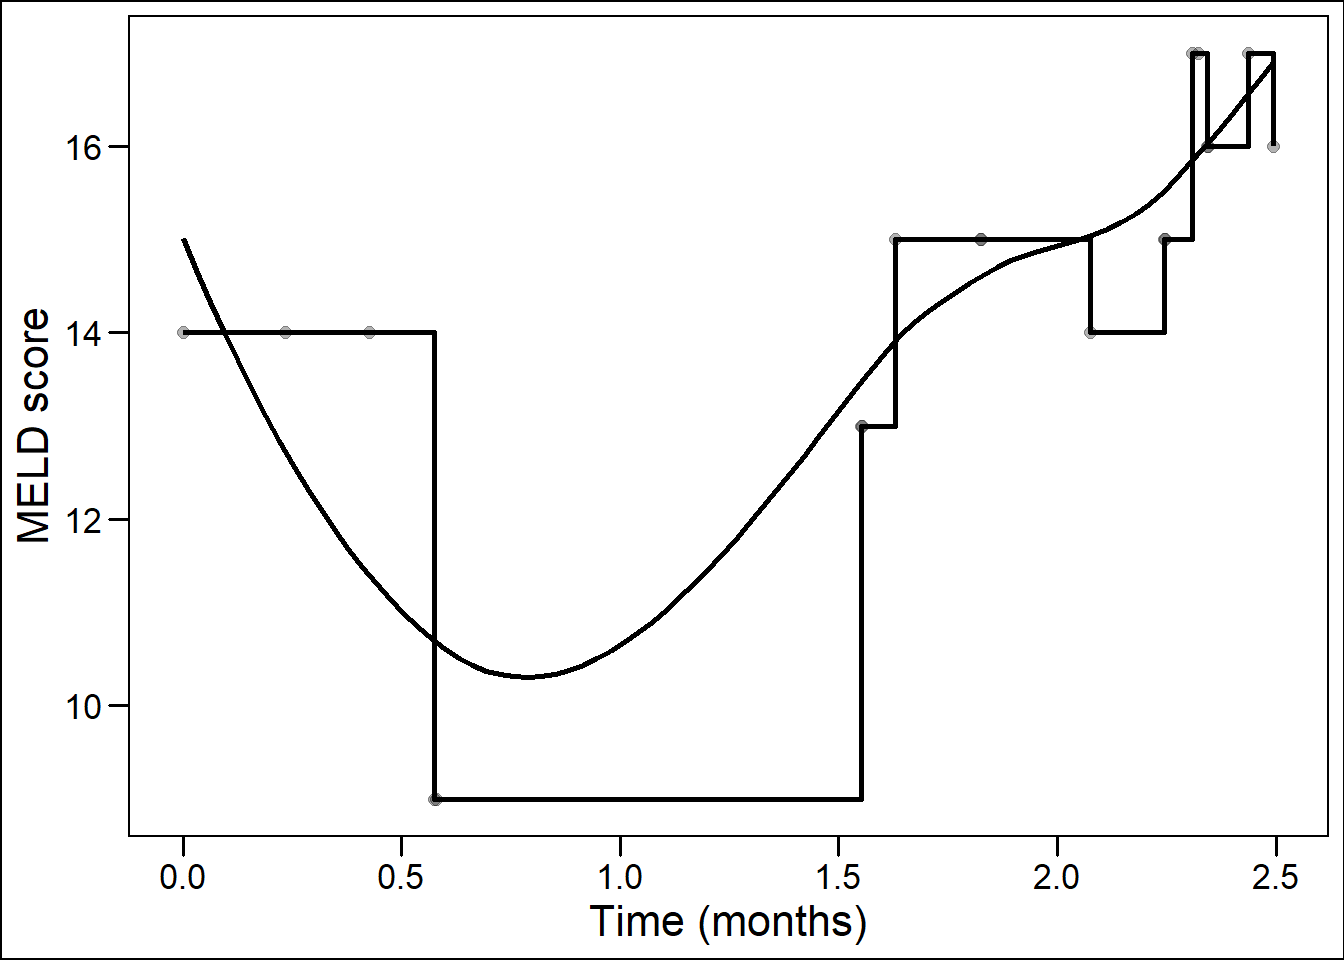
\includegraphics{thesis_files/figure-latex/disc-fig1-1.pdf}
\caption{\label{fig:disc-fig1}Staircase versus smooth representation of disease over time.}
\end{figure}

However, it is clinically evident that the condition of a patient and the liver disease are not constant until a new moment of measurement. Instead, disease develops continuously, as a smooth and non-linear trajectory. We configured JMs to estimate disease as a smooth continuum over time with interpolation of trajectories between measurements. At and between measurements, not the last measured value was assumed, but the `true' underlying value. For the abovementioned example, the JM would estimate values for each moment in time between day 0 and 60. Crucially, the model considered that measurements from the same patient were more related than measurements between patients. TDC models ignore this correlation.

Another advantage of extrapolating the true underlying trajectory is that missing values are filled in. Missing values therefore have less effect on estimated survival. We therefore believe that JMs are better suited for real-life cohort data, where disease is continuously developing and where measurements are correlated and can be missing. The performance of JMs versus TDC models was previously assessed in small and theoretical simulation studies, where JMs showed significantly improved performance over TDC models.\textsuperscript{33--35} However, JMs were never applied to large cohorts of patients nor to the field of LT. In \textbf{Chapter \ref{chap-jm}}, \textbf{Chapter \ref{chap-aclfjm}} and supplement \textbf{Chapter \ref{chap-rolejm}}, we therefore investigated JMs as alternatives for survival prediction in LT candidates.

\hypertarget{joint-modeling-disease-and-survival-over-time}{%
\subsection*{Joint modeling disease and survival over time}\label{joint-modeling-disease-and-survival-over-time}}
\addcontentsline{toc}{subsection}{Joint modeling disease and survival over time}

In \textbf{Chapter \ref{chap-jm}}, we fitted JMs to waiting list data of the Eurotransplant and UNOS regions. The JMs modeled average and individual MELD scores and considered both the value of MELD(-Na) and its rate of change at each moment in time. For the first time, liver disease was considered as developing entity within each patient on the waiting list.

\hypertarget{underlying-meld-value}{%
\subsubsection*{Underlying MELD value}\label{underlying-meld-value}}
\addcontentsline{toc}{subsubsection}{Underlying MELD value}

The observed, that is measured, values of MELD(-Na) scores have been used in liver graft allocation for 20 years. The JM uses these observed measurements to estimate the `true' underlying disease trajectory. The model can therefore assume a different MELD(-Na) score than is observed for each patient. For example, for actively listed LT candidates in the Eurotransplant region between 2007-2018, the median measured value of MELD at the start of listing was 15 ( Table \ref{tab:jm-tab1} ). However, the JM assumed a baseline MELD value of 17.8, which is notably higher. In addition, for each patient, the JM considered the individual deviation from the average MELD(-Na) score at a given moment in time. This placed patients in context to the population average. The individual deviations from the average were also used as prognostic information in survival prediction. Naturally, the question arose whether this underlying disease severity should be used over actually measured disease.

\hypertarget{prediction-performance-based-on-underlying-trajectories}{%
\subsubsection*{Prediction performance based on underlying trajectories}\label{prediction-performance-based-on-underlying-trajectories}}
\addcontentsline{toc}{subsubsection}{Prediction performance based on underlying trajectories}

Interestingly, when predicting waiting list survival, the JM outperformed MELD both at baseline and during follow-up. This implied that 1) the JM-estimated underlying disease severity better corresponded with survival than observed MELD values and 2) using individual deviation from the population average added prognostic information. The estimated underlying disease trajectory is less sensitive to missingness or errors. JMs can however be severely biased if they are mis-specified, particularly in the specification of longitudinal trajectories.\textsuperscript{33} Therefore, we considered multiple configurations of spline-based and linear mixed effect models (longitudinal part of the JMs) and assessed their fit through Akaike information criterion (AIC) values. Most notably, the use of spline-based instead of linear-approximated patient trajectories greatly improved model fit.

Over time more waiting list data per patient typically becomes available. Therefore, after listing, the JM predictions became increasingly accurate within each patient as follow-up increased, which contrasts to MELD(-Na). Little attention is given in literature to the fact that MELD is a Cox model constructed and validated to first listing data.\textsuperscript{7,9,10} However, most patients on the waiting list are months away from first listing. When assessing JM and MELD performance over time, a decline in discrimination and accuracy was shown. The patients who survived longest on the waiting list despite their MELD scores likely had a better condition beyond what MELD measured, or vice versa. However, since only MELD was measured, over time it became more difficult to predict survival in the resulting population. Still, JM performance was significantly better than MELD performance for most follow-up times. Also, in our analysis, all patients started from the same moment in time (first listing). However, on the actual waiting list, patients are constantly added and removed. In other words, survival prediction for liver graft allocation is based on cross-sections, not a cohort. In real waiting list data, MELD's discrimination is therefore likely to be lower, as the sickest patients are transplanted quickly and ranking the remaining less ill patients is more difficult. The JM accuracy increases with more available measurements over time. Because of this, we would not expect a similar decrease in performance if the JM would be applied to the actual waiting list.

\hypertarget{joint-modeling-acute-on-chronic-liver-failure}{%
\subsection*{Joint modeling acute-on-chronic liver failure}\label{joint-modeling-acute-on-chronic-liver-failure}}
\addcontentsline{toc}{subsection}{Joint modeling acute-on-chronic liver failure}

\hypertarget{aclf-and-meld-na}{%
\subsubsection*{ACLF and MELD-Na}\label{aclf-and-meld-na}}
\addcontentsline{toc}{subsubsection}{ACLF and MELD-Na}

Liver disease is constantly changing. In clinical practice, the rate at which a patient changes directly influences medical urgency and possible intervention. This might be especially true for patients with acute-on-chronic liver failure (ACLF). ACLF is characterized by initially stable and chronic liver disease, which rapidly deteriorates after a predisposing event and leads to multi-organ failure and often death.\textsuperscript{36} Timely transplantation can save a subset of these patients,\textsuperscript{37} but MELD-Na underestimates ACLF mortality and therefore the need for transplantation.\textsuperscript{38,39}

In supplement \textbf{chapter \ref{chap-rolejm}}, we hypothesized that JMs would be suited for predicting ACLF survival.\textsuperscript{40} First, because each individual patient's condition can change rapidly. Therefore, it is relevant to predict survival based on both past and current data. It is also relevant to place the individual disease and survival in context to the population average. Second, by using both measured disease severity and its rate of change over time, the acceleration in ACLF severity is linked to future survival. Third, updating future predictions at each new measurement is relevant in patients with increasing disease severity.

In \textbf{Chapter \ref{chap-aclfjm}}, we approximated liver disease severity in ACLF patients based on repeated MELD-Na values, corrected for baseline ACLF grade and other predictors (sex, age, presence of cirrhosis, life-support dependency, and presence of bacterial peritonitis). However, predicting ACLF survival based on MELD-Na measurements was suboptimal. This is because ACLF involves inflammation and multi-organ failure,\textsuperscript{36} which are not captured by MELD-Na scores. Therefore, ACLF survival prediction could be improved further by modeling more organ system functions over time. Survival prediction based on simultaneous consideration of multiple organ systems is possible in multivariate JMs. It would make sense to separately consider the role of each organ system. Unfortunately, such data is not readily available for both the Eurotransplant and UNOS regions. Therefore, like others,\textsuperscript{37,38,41} we could only correct for ACLF grade at baseline. However, within the European Foundation for the study of Chronic Liver Failure (EF CLIF) consortium data, longitudinal CLIF ACLF scores measurements per patients could be available. Therefore, future application of JMs in this data might result in JMs that better represent changes in ACLF and let failure of each organ system correlate to mortality.

\hypertarget{underlying-meld-rate-of-change}{%
\subsubsection*{Underlying MELD rate of change}\label{underlying-meld-rate-of-change}}
\addcontentsline{toc}{subsubsection}{Underlying MELD rate of change}

Despite using MELD-Na as basis, we still hypothesized that improvement was possible, mainly because baseline ACLF severity and MELD-Na rate of change would be considered. For the rate of change, the term `slope' is often used, as the rate of change is the derivative of the function of MELD-Na values over time. The concept of MELD-Na's rate of change (or slope) over time is not new. Most notably, delta-MELD has been proposed previously.\textsuperscript{25} However, the slope generated by the JM differs notably from delta-MELD. Firstly, the JM slope is based on the assumed true underlying disease development (see above). Secondly, the JM slope is the derivative of the measured value at one specific moment in time. In contrast, delta-MELD is defined as the difference between the current MELD score and the lowest MELD score in the previous 30 days, divided by the number of days between the current and lowest scores.\textsuperscript{25} Thus, the obtained delta-MELD slopes are averaged over a varying number of days for different patients and time points. Also, using the lowest previously measured value overestimates the rate of change, unless the previous value actually is the lowest. This way, delta-MELD could indicate increasing disease severity even though a patient was in stable condition, see Figure \ref{fig:disc-fig2}. Basing treatment decisions on such estimates therefore seems inappropriate. In the example below, the JM slope would be approximately horizontal at 30 days and therefore the instantaneous slope at each moment is a better representation changing disease.

\begin{figure}
\centering
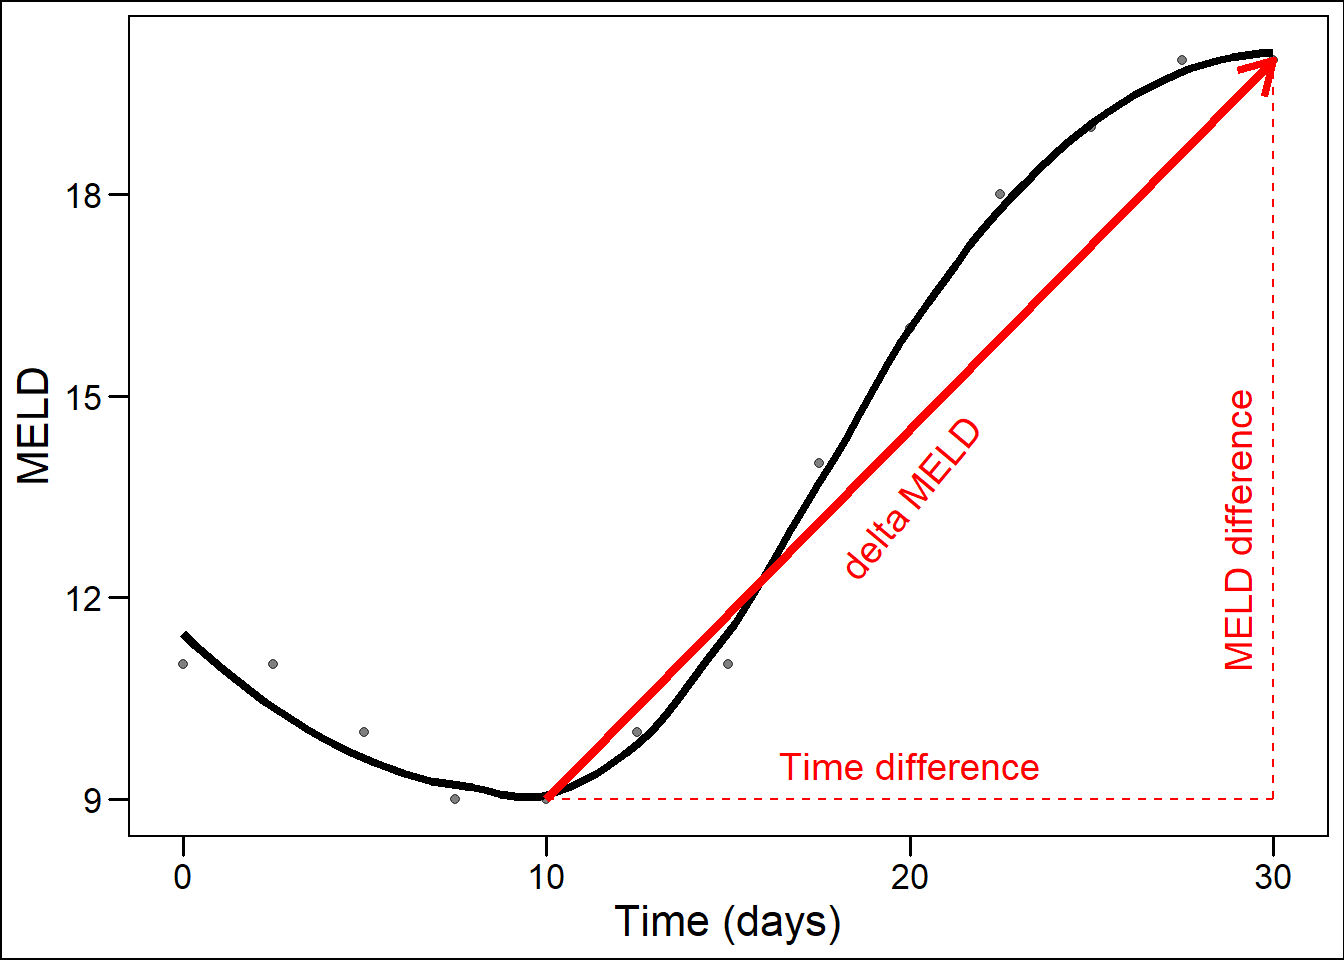
\includegraphics{thesis_files/figure-latex/disc-fig2-1.pdf}
\caption{\label{fig:disc-fig2}Illustration of delta-MELD slope overestimation of disease increase.}
\end{figure}

Lastly, the effect of delta-MELD on waiting list mortality depends on the number of previous MELD measurements.\textsuperscript{42} This causes bias for survival prediction on the LT waiting list, as the severity of disease determines the number of measurements. For example, a clinician could increase the frequency of measurement after a patient's disease worsens, or vice versa. Thus, measuring MELD and delta-MELD in sick patients corresponds with death, but an improvement would likely be less easily observed. Therefore, Delta-MELD depends on the number of measurements, which causes bias that will increase its apparent usefulness.\textsuperscript{26} Despite this bias, the concept of delta-MELD is used often.\textsuperscript{5,28,43--48} In our view, this stipulates the need to adequately incorporate MELD's rate of change in survival prediction. The JM is not biased by the number of measurements, as it estimates a continuous underlying trajectory. Still, with increasing measurements available, the trajectory of the patient will be more accurately reflected.

\hypertarget{personalized-predictions}{%
\subsubsection*{Personalized predictions}\label{personalized-predictions}}
\addcontentsline{toc}{subsubsection}{Personalized predictions}

Because JMs consider both the average and individual development of disease, survival predictions can be personalized. Consider that a Cox model uses coefficients, derived from a studied population, to predict outcome. These coefficients can be viewed as the average parameter-mortality relationships of a studied population. However, applying these coefficients on an individual level will give only an average prediction of survival. A patient could ask her physician: `` \emph{How long will I survive with my current disease?}'' Based on a MELD score, e.g.~20, the physician could give a prognosis estimate based on population averages counted from baseline. In other words, a correct answer would be: `` \emph{If there would be 100 patients with your MELD score 20, we estimate that on average 10\% will have died within three months after first waiting list registration.}'' After this clarification, questions and uncertainty remain for the patient and possibly also for the physician, because of several reasons.

First, the patient does not know how `average' she is, that is how well the average parameter-mortality relation will apply to her. This is why considering individual patient trajectories through joint-modeling is valuable. Second, the patient is most likely not at the moment of first registration but beyond that, at some later point in time, which is why it is better to use accumulating data over time and update predictions accordingly. Third, clinicians could also miss that MELD's predictions were only validated on baseline populations.\textsuperscript{7,9,10}

We believe that the personalized predictions can benefit both the patient and the clinician. The main reason being that the patient is recognized as unique entity and is not abstracted into population averages. The clinician can also be more confident that the predicted prognosis applies to the individual patient. Therefore, personalized JM predictions were made available at \url{https://predictionmodels.shinyapps.io/meld-jm/}.

\hypertarget{part-iii-survival-with-and-without-transplantation-1}{%
\subsection*{Part III: Survival with and without transplantation}\label{part-iii-survival-with-and-without-transplantation-1}}
\addcontentsline{toc}{subsection}{Part III: Survival with and without transplantation}

\hypertarget{benefit-from-liver-transplantation}{%
\subsection*{Benefit from liver transplantation}\label{benefit-from-liver-transplantation}}
\addcontentsline{toc}{subsection}{Benefit from liver transplantation}

The final part of this thesis studies a simple question: \emph{``does transplantation improve survival?''} In \textbf{Chapter \ref{chap-benefit}}, we investigated whether LT \emph{caused} survival improvement for patients on the waiting list. The difficulty is that such causal effects, that is the difference between transplanting and not transplanting, cannot be observed, as each patient is either transplanted or not. It would be considered unethical to conduct a randomized trial on LT survival benefit. Therefore, counterfactual waiting list survival of transplanted patients was estimated through inverse probability of censoring weighting (IPCW) analysis.\textsuperscript{49} Benefit scores were calculated as the difference between survival with and without LT.

We used sequential stratification and IPCW to predict counterfactual waiting list survival, which is the waiting list survival of a transplanted patient if LT would not have been done. We applied these techniques because patients on the waiting list are transplanted after baseline and the donor graft is allocated depending on the severity of disease. See Figure \ref{fig:disc-fig3} below, where four hypothetical patients on the waiting list are shown (three severely ill, one less ill). In this example, patient 2 is dependently censored at transplantation and therefore survival of remaining and comparable patients is given more weight. Each patient was listed at a different point in time (t0) and therefore spent a variable amount of time waiting at the cross-section. Survival is counted from the moment of cross-section and all patients receive equal weights (w=1). Due to high disease severity, patient 1 died before a liver graft became available. Patient 2 survived long enough and was transplanted. After transplantation of patient 2, patient 3 received more weight (w=2) to compensate for the missing survival time of patient 2 after censoring. Patient 4 (medium MELD) did not receive higher weight as its condition was not comparable to patient 2.

\begin{figure}
\centering
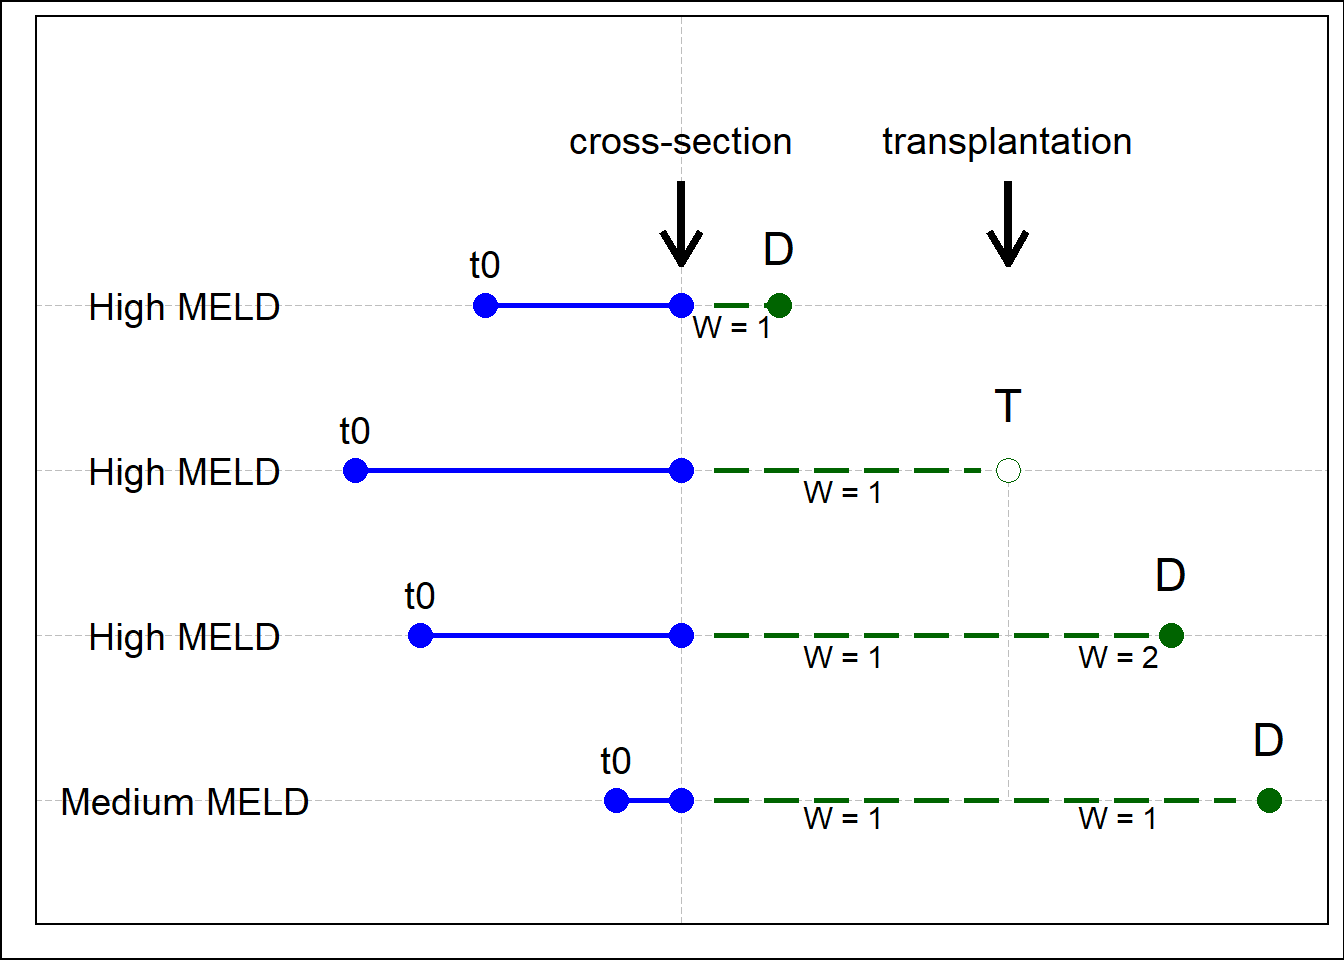
\includegraphics{thesis_files/figure-latex/disc-fig3-1.pdf}
\caption{\label{fig:disc-fig3}An illustration of IPCW. Note the change from w=1 to w=2 for patient 3. D: death, T: transplantation.}
\end{figure}

\hypertarget{validity}{%
\subsubsection*{Validity}\label{validity}}
\addcontentsline{toc}{subsubsection}{Validity}

In the literature, benefit is often defined as the difference between post-transplant survival and waiting list survival counted from baseline.\textsuperscript{50--54} The idea is to match patients with a similar disease state (e.g., MELD score) either at waiting list registration or transplantation. However, this definition of benefit assumes that two different patients at two different moments in time will yield survival curves that can be compared. We argue against these assumptions. Firstly, the fact that two patients have the same MELD score, perhaps with some more similarities like age and sex, does not make their state of disease comparable. We showed this to be true in \textbf{Part II}, where we showed that 1) previous disease development is different between two persons and 2) the rate of change in disease severity significantly influences future survival. This is perhaps best illustrated in Figure \ref{fig:jm-fig1}. Secondly, following from the previous arguments and the fact that liver disease typically progresses over time, survival predictions based on two different moments in time should not be compared to estimate benefit. Third argument is that the decision to transplant or not is made at the moment of liver graft offering, not baseline. Fourth, the fact that MELD and other predictors can be measured at baseline or at transplantation does not mean that it is right to use only these, which is the law of the instrument.\textsuperscript{55} Therefore, by comparing survival within patients based on previous disease and slope, we provided a more precise and valid definition of patient disease. Still, the validity of the time-dependent Cox benefit estimates could have been improved further by using JMs to better define disease severity.

\hypertarget{reliability}{%
\subsubsection*{Reliability}\label{reliability}}
\addcontentsline{toc}{subsubsection}{Reliability}

The reliability of benefit estimates was also improved. Firstly, because we estimated survival from a certain calendar moment in time (cross-section). This is important, as liver grafts are offered to cross-sections of patients, where each patient has previously waited a variable amount of time and survival is predicted from that moment on. Counting survival from baseline instead makes all patients start from the same moment in time. Secondly, we used weighting to 1) correct waiting list survival for dependent censoring bias and 2) estimate waiting list survival as if LT was not available as treatment. Careful consideration of which question is answered by which statistical method is important when estimating benefit.\textsuperscript{56} In clinical terms: an example is making a distinction between the survival before LT and survival without LT, which are very different (Figure \ref{fig:benefit-fig1a} ).

Careful consideration argues against using competing risks (CR) analyses to approximate waiting list survival without LT.\textsuperscript{50--52} CR analysis estimates survival before LT and should be used to evaluate waiting list outcomes: transplantation, death, or removal.\textsuperscript{56} It would be wrong to base allocation on CR-predicted future waiting list survival. To illustrate, consider a patient with MELD 40 (very ill) and a patient with MELD 20 (reasonably ill). A physician might predict correctly that the MELD 40 patient has a (much) higher chance of receiving a LT the next 90 days than the MELD 20 patient, as transplant chances increase with disease severity. In CR reasoning, we would then argue that the risk of death for the MELD 40 patient is lowered, as transplantation competes with death. However, it would be perverse to decrease allocation priority based on this reasoning, as the high chance of transplantation for the MELD 40 patient is a result of the high risk of death. Instead, priority should be based on the risk of death without LT,\textsuperscript{49,56} which we properly modeled using censorship with adjustment for dependent censoring.

By correctly modeling waiting list survival without LT in the last part of this thesis, we must acknowledge, due to progressive insight, that the reliability of the previous survival prediction models in \textbf{Part I} and \textbf{II} could have been improved further. We modeled survival in a censorship framework but did not adjust dependent censoring bias through IPCW. This should have been done, as the priority for LT depends on MELD and the Cox model assumes that censored patients have the same chance of dying as patients who remain on the waiting list, which is not the case for transplanted patients. Since transplantation chances increase with MELD, the sickest patients typically spend the least time on the waiting list, because they are transplanted (and censored) more frequently and faster. Through IPCW, after a (high MELD) patient is transplanted, more weight is given to the remaining and comparable (high MELD) patients, who can survive some more time on the waiting list. Censoring without weights, which MELD(-Na) does, therefore leads to an increasing underestimation of mortality for patients with increasing disease severity, as death is more frequently prevented through transplantation (and after censoring outcomes and survival times are unknown). In other words, by using the unweighted MELD(-Na), current liver allocation is biased where it matters most, as it underestimates mortality in the sickest patients.

\hypertarget{logical-continuation}{%
\subsubsection*{Logical continuation}\label{logical-continuation}}
\addcontentsline{toc}{subsubsection}{Logical continuation}

Although the clinical relevance of causal models is evident, a problem is that their prediction performance cannot be assessed (yet).\textsuperscript{57} Consider for example calibration, where predicted and observed risks are compared. This comparison cannot be done, as counterfactual waiting list survival is not observed. We are however confident about the obtained estimates. Firstly, because simulation studies showed that the used methods are valid.\textsuperscript{49,58} Secondly, the future waiting list survival estimates of transplanted patients are a logical continuation of observed and corrected waiting list survival. An illustrative analogous example from mathematics is analytic continuation, where the domain of a function is extended in the only way possible that is preserving certain requirements. Consider Figure \ref{fig:disc-fig4}A below, where the lines in the right half of the plot represent a certain function (Riemann Zeta function, source: \url{https://www.3blue1brown.com/lessons/zeta}). Only the right half is shown, as only this side can be defined by the function. The left half of the plot in Figure \ref{fig:disc-fig4}B shows the analytically continued right half, which is continued from the right based on requirements such as line angles. However, the left half cannot be defined by the function that plots the right half, even though its continuation is logical and can be visualized. This is analogous to estimating without LT survival (left half) based on observed waiting list survival (right half), which is a logical continuation based on available data, but by definition cannot be observed nor validated.

\begin{figure}

{\centering \subfloat[Right half can be defined\label{fig:disc-fig4-1}]{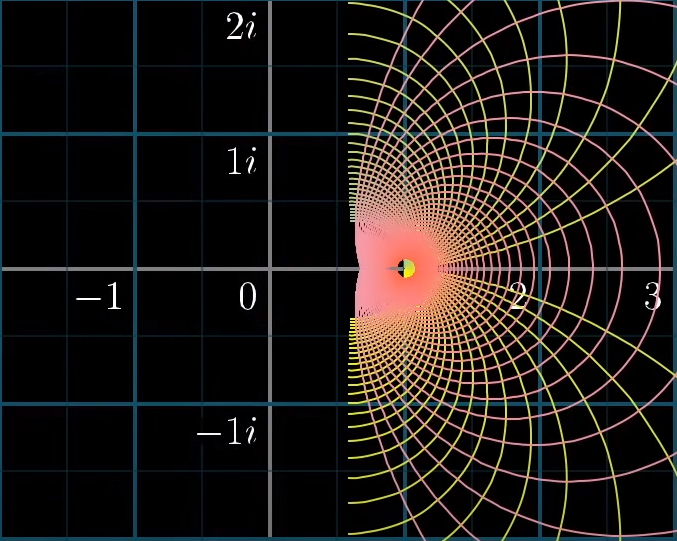
\includegraphics[width=0.5\linewidth]{figures/discussion/riemann right} }\subfloat[Left half cannot be defined, but it can be continued.\label{fig:disc-fig4-2}]{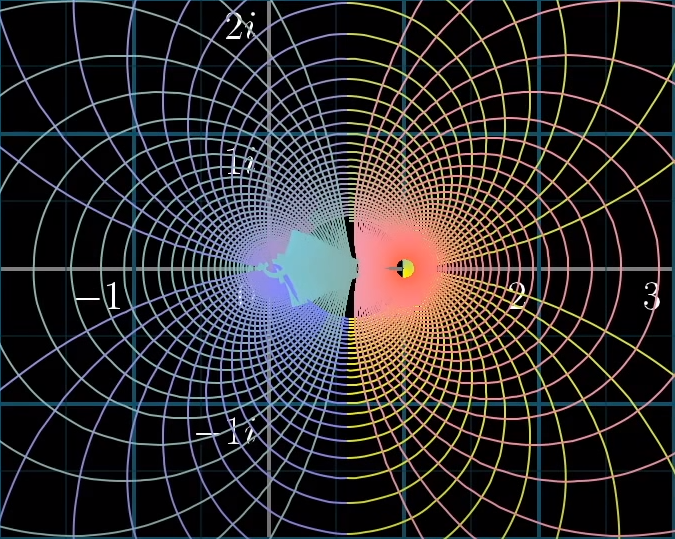
\includegraphics[width=0.5\linewidth]{figures/discussion/riemann left and right} }

}

\caption{Analytic continuation of the Riemann zeta function.}\label{fig:disc-fig4}
\end{figure}

Although causal models currently cannot be validated, benefit allocation policy has been based on these methods, most notably the MELD-Na implementation for patients with MELD\textgreater11 and UK benefit-based allocation.\textsuperscript{6,30,59} We believe that the predicted survival without LT as possible treatment best serves as guide for transplantation assignment in future patients.\textsuperscript{56,57,60}

Further improvements of causal liver allocation models are possible. We performed a retrospective study of benefit. However, for prospective use in allocation, IPCW could be replaced by IPTW, that is inverse probability \emph{treatment} weighting. IPTW differs from IPCW in that both survival with and without LT are estimated as future hypothetical risks, whereas in the IPCW analysis of \textbf{Chapter \ref{chap-benefit}} the with LT survival was retrospectively observed. IPTW further approximates clinical decision making based on expected outcomes with and without transplantation, as in reality both outcomes are hypothetical at the moment of liver graft offering. This requires clinicians to be comfortable with basing treatment decisions on hypothetical risks from models that cannot be validated (yet). However, this is what experienced clinicians do intuitively when evaluating an offered donor liver graft for a LT candidate. Indeed, the statistical machinery required to approximate clinical decision making is complex. This highlights the capabilities and intuition required from an experienced physician who is faced with the decision to transplant or not.

\hypertarget{two-principles}{%
\subsubsection*{Two principles}\label{two-principles}}
\addcontentsline{toc}{subsubsection}{Two principles}

We compared LT survival benefit of patients with and without HCC. This comparison is relevant because different allocation principles are applied to patients with and without HCC. The group of HCC patients is intended to be exemplary for other exception patients. With increasing HCC incidence,\textsuperscript{61} already inequal LT access might be worsened further.\textsuperscript{12} For non-HCC patients, LT listing is based on expected waiting list survival, or the principle of urgency (sickest first). HCC patients are listed based on Milan criteria, which represent acceptable post-transplant survival.\textsuperscript{62} Considering post-transplant survival is the principle of utility, which ignores HCC waiting list survival and alternative pre-LT HCC treatment options.\textsuperscript{63} Moreover, instead of patient characteristics, artificial exception points are used to express HCC waiting list priority, which further worsened the already inequal LT access between non-HCC and HCC patients.\textsuperscript{50,64,65} Lastly, HCC patients within Milan criteria and within one region are prioritized on waiting time, which is inherently flawed, as waiting longest does not equal to highest waiting list mortality.\textsuperscript{66,67} To resolve these issues, we proposed the use of survival benefit as single equalizing metric. Previous simulation showed that benefit-based allocation resulted in more life-years gained from the same number of available liver grafts.\textsuperscript{30}

However, if physicians and policy makers do not endorse benefit as metric, at least (non-)HCC waiting list survival should be estimated by a single pre-transplant survival model, which could be similar to our proposed weighted waiting list model. The use of actual patient characteristics to estimate both waiting list and post-transplant survival removes the need for the inherently flawed exception points. With the availability of HCC waiting list survival prediction models, there is no need for arbitrary and artificial inadequacy through exception points, as these are solely needed to compensate MELD(-Na)'s inability to predict waiting list survival in patients with preserved liver function. Policy and research should focus on collecting data and establishing models that adequately predict survival. This would remove the ongoing time-consuming arbitrary changes required for the exception point system. Survival prediction and liver graft allocation should be based on actual patient characteristics, not arbitrary points.

\newpage
\pagecolor{black}
\color{white}

\hypertarget{future-perspectives}{%
\chapter{Future perspectives}\label{future-perspectives}}

\newpage
\nopagecolor
\color{black}

\hypertarget{simulation}{%
\subsection*{Simulation}\label{simulation}}
\addcontentsline{toc}{subsection}{Simulation}

Throughout this thesis, several methods were applied to estimate new model impact on the LT waiting list. We used reclassification tables, new-to-old score differences, or estimated changes in waiting list priority. These methods were used because reviewers and policymakers requested evidence of possible model impact on current waiting list outcomes. Although understandable, it is difficult and likely impossible to reliably estimate the impact of a new model on the allocation system. The best way to evaluate the effects of a new model is to implement it. The next best option is evaluation through simulation. For the Eurotransplant region, a simulation program is currently missing. An important future direction of research could therefore be the construction of what could be called the Simulation of the Eurotransplant Liver Allocation System (SELAS). SELAS would improve both Eurotransplant allocation research and policy. It would also help Eurotransplant regain its leading role in organ allocation and development. Realization of SELAS seems feasible given the existing collaboration between Eurotransplant International Foundation and the Technical University Eindhoven, as the latter has considerable experience with simulation models. The longstanding cooperation between Eurotransplant and the Leiden University Medical Center would then ensure integration of allocation, statistical methodology, and clinical knowledge.

In the U.S.A., a liver simulation program is available, that is the Liver Simulated Allocation Model (LSAM). LSAM lets users change existing allocation rules and simulate the effects in historical US data. Indeed, US allocation research is often complemented by simulation evidence. Still, simulated results should be interpreted with care. Evaluation of LSAM showed that although trends were adequately estimated, exact numbers of waiting list deaths and transplants were over- and underestimated, respectively.\textsuperscript{68} Also, simulation performance was significantly worse for pediatric patients,\textsuperscript{69} which indicates that simulations might be unreliable for yet undefined subgroups.

Even simulation programs have limitations. Therefore, researchers should rely on their methodology and clinical experience. Consider for example the refit coefficients in \textbf{Chapter \ref{chap-refit}}. We presented significant improvements in fit, discrimination, and accuracy. Although these metrics are important evidence, improvement was most intuitively shown through visual representation of new and old coefficients Figure \ref{fig:refit-fig3}. These clearly showed that reMELD(-Na) better represents the Eurotransplant population and therefore will likely better predict risk in future LT candidates. Simulation of evidence therefore has a role in the path of implementation, but sound methods and reasoning should be considered most important.

\hypertarget{new-model-implementation}{%
\subsection*{New model implementation}\label{new-model-implementation}}
\addcontentsline{toc}{subsection}{New model implementation}

Possibilities are investigated to alleviate the shortage of available donor organs, such as more liberal donor criteria, living donation, machine perfusion, organoids, and xenotransplantation. Whatever improvements might be made, survival prediction will remain paramount to decide which patient should be treated. For example, with machine perfusion techniques, a larger number of liver grafts will likely become available and will be preserved longer outside the donor. This could imply more widespread allocation of organs to find the best match with the recipient. Also, with more time available, more complex calculations could be done to estimate outcomes of possible donor-recipient combinations. These calculations could be based on causal inference models, JMs, or ideally a combination of both.

For now, the shortage of donor organs persists. As mentioned, currently the principle of urgency is used for liver allocation, by prioritizing the sickest patients first. Eurotransplant has maintained this basis since 2006. In this thesis, we showed that significant improvements in survival prediction are possible. Understandably, reasons beyond clinical relevance and statistical significance determine model implementation. Because of (inter)national interests within Eurotransplant, changes in allocation are not easily implemented. Still, in our view, refit MELD (reMELD) would be relatively easy to implement, as no changes in the data structure of Eurotransplant would be required. We therefore urge Eurotransplant policy makers to consider that the refit models were a significantly better fit to the current Eurotransplant population, that ranking patients from most to least ill (discrimination) was significantly improved, and that refit model mortality risk estimates were more accurate. Implementation of (refit) MELD-Na would also not be very difficult, since sodium is a readily available laboratory measurement, that is almost always assessed in combination with creatinine. Again, the significant prediction improvements should form sufficient rationale for further allocation improvements.

Other additions to MELD could also be considered, such as serum albumin, von Willebrand factor and C-reactive protein.\textsuperscript{18,20,70} A problem is that these variables are not collected within Eurotransplant. Several aspects of MELD, that are not evidence based, can however be improved without changing existing data registries.\textsuperscript{19} Arguably one of the most important and counter-intuitive aspects is MELD's upper bound of 40, which means that patients with MELD\textgreater40 receive a score of 40. Therefore, allocation stops considering disease severity in the sickest patients. Already in the first validation study of MELD, MELD's relation to 90-day risk of death was plotted and showed an increasing waiting list mortality above MELD 40.\textsuperscript{7} Recent evaluation confirmed this finding, without increased post-transplant mortality for recipients with MELD\textgreater40.\textsuperscript{71} It therefore makes clinical sense to remove the upper border of MELD in order to improve allocation for the sickest patients. Other suggestions to improve MELD were mentioned previously in this thesis, like removing arbitrary lower and upper bounds and using survival probabilities as primary metric.

The implementation of JMs for allocation would require more effort. Eurotransplant would need to ensure that longitudinal data of each listed patient is available every time a liver graft is offered. However, if using one measurement per patient is possible, it should also be possible to use multiple, as these longitudinal data are stored by Eurotransplant. The computation of JM survival predictions would require notably more time than calculating MELD, as simulations are done for each patient. However, we believe that the advantages of correctly specified JMs are convincing. Also, although the JMs were trained in large patient cohorts, their practical application for the Eurotransplant waiting list would mean calculating survival for several hundred patients, which is done within minutes. Considering previous and current data for each patient on the waiting list would be a major improvement.

\hypertarget{from-urgency-to-benefit}{%
\subsection*{From urgency to benefit}\label{from-urgency-to-benefit}}
\addcontentsline{toc}{subsection}{From urgency to benefit}

Deciding how to allocate scarce medical interventions is relevant, as the recent COVID pandemic has shown for vaccines and ICU beds. The COVID pandemic also showed that with increasing resource scarcity, a shift in allocation principle could be warranted, that is from a `first come first served' to a benefit-based approach.\textsuperscript{72}

In the field of LT, organ demand persistently exceeds supply, which argues against sickest-first allocation.\textsuperscript{67} This is because prioritizing the sickest ignores currently less ill patients that might gain more from treatment or who could be worse off in the future as disease progresses. Therefore, sickest-first allocation can only be just if the scarcity is temporary, which is not the case. This does evoke questions on how to handle high-urgency patients, as these patients are the pinnacle of urgency-based allocation and receive priority over other patients that have higher waiting list mortality.\textsuperscript{31,49,73} Another extreme of urgency are multi-organ transplants. These possibly save only one life, whereas each of the organs could have saved a patient. Saving more lives is arguably more just. Finally, re-transplantations would require similar reconsideration of urgency and benefit,\textsuperscript{73} as the highest priority is given to patients who might gain little and, perhaps more importantly, the liver is then denied to another recipient. Although benefit will not resolve all allocation issues, it is an inherently more just and therefore a better principle than urgency alone.\textsuperscript{67}

We devised methods that predict survival benefit from LT. This opens the possibility for the change from urgency- to benefit-based allocation. It is however important to recognize that US data were used for the calculation of benefit. These US data encompass more LT candidate variables, that allow better estimation of future waiting list survival. Currently, Eurotransplant registers fewer LT candidate variables. It is easy to see that this will cause delay in allocation development, especially compared to other regions. This is arguably already the case, as No major revision of MELD allocation has been done by Eurotransplant since 2006. During this period, survival prediction models in US liver graft allocation were investigated and significantly improved. In our view, Eurotransplant should strive for a data registry structured much like UNOS, which allows researchers easy access to anonymized data. This in turn generates evidence upon which policy can be based. In our view, Eurotransplant should also provide a central platform where professionals and patients can gain insight in allocation policy and evidence. Transparency created through interactive statistics and accessible prediction models would greatly improve Eurotransplant's scientific basis and would perhaps place more trust in the organization. Most importantly, patients deserve to know their estimated prognosis of waiting for or accepting an organ. To this end, in this thesis, we provided several prediction models in interactive online applications. The aim was to increase insight for both clinicians and patients.

Another possible solution for the advancement of liver allocation, despite the missing data across Eurotransplant, could be detailed national allocation based on more detailed hospital data. This allocation could be either benefit- or urgency-based, as long as one model is used to calculate future waiting list survival, preferably corrected for dependent censoring. Most organs are allocated nationally, that is 83.4\% of MELD-allocated liver grafts in Belgium, Germany, and The Netherlands ( \emph{data not published} ), which also ignores possibly sicker recipients abroad. Therefore, it seems feasible to abandon the sickest-first principle and to implement benefit-based allocation on a national level. This way, each country would be responsible for the method and accuracy of its survival prediction and subsequent allocation. International organ exchange would then be based on Eurotransplant standards.

\hypertarget{conclusion-5}{%
\section*{Conclusion}\label{conclusion-5}}
\addcontentsline{toc}{section}{Conclusion}

In conclusion, this thesis investigated survival prediction models in the setting of LT, where organ scarcity and allocation necessitates continuous development of such methods. Statistically significant and clinically relevant advancements were demonstrated that could improve liver allocation through better survival prediction for patients on the waiting list.

\newpage
\linespread{1}
\small

\chaptermark{References}

\hypertarget{references-6}{%
\section*{References}\label{references-6}}
\addcontentsline{toc}{section}{References}

\begin{enumerate}
\def\labelenumi{\arabic{enumi}.}
\tightlist
\item
  Alukal JJ, John S, Thuluvath PJ. Hyponatremia in Cirrhosis: An Update. Am J Gastroenterol. 2020;115(11):1775-1785. \url{doi:10.14309/ajg.0000000000000786}
\item
  Londoño MC, Guevara M, Rimola A, et al.~Hyponatremia Impairs Early Posttransplantation Outcome in Patients With Cirrhosis Undergoing Liver Transplantation. Gastroenterology. 2006;130(4):1135-1143. \url{doi:10.1053/j.gastro.2006.02.017}
\item
  Dawwas MF, Lewsey JD, Neuberger JM, Gimson AE. The Impact of Serum Sodium Concentration on Mortality After Liver Transplantation: A Cohort Multicenter Study. Liver Transplant. 2007;13(5):767-768. \url{doi:10.1002/lt}
\item
  Leise MD, Yun BC, Larson JJ, et al.~Effect of the Pretransplant Serum Sodium Concentration on Outcomes Following Liver Transplantation. Liver Transplant. 2014;14(20):687-697. \url{doi:10.1002/lt}
\item
  Nagai S, Chau LC, Schilke RE, et al.~Effects of Allocating Livers for Transplantation Based on Model for End-Stage Liver Disease-Sodium Scores on Patient Outcomes. Gastroenterology. 2018;155(October):1451-1482. \url{doi:10.1053/j.gastro.2018.07.025}
\item
  Sharma P, Schaubel DE, Goodrich NP, Merion RM. Serum Sodium and Survival Benefit of Liver Transplantation. Liver Transplant. 2015;21:308-313. \url{doi:10.1002/lt}.
\item
  Singal AK, Ong S, Satapathy SK, Kamath PS, Wiesner RH. Simultaneous liver kidney transplantation. Transpl Int. 2019;32(4):343-352. \url{doi:10.1111/tri.13388}
\item
  Malinchoc M, Kamath PS, Gordon FD, Peine CJ, Rank J, Ter Borg PCJ. A model to predict poor survival in patients undergoing transjugular intrahepatic portosystemic shunts. Hepatology. 2000;31(4):864-871. \url{doi:10.1053/he.2000.5852}
\item
  Kamath PS, Wiesner RH, Malinchoc M, et al.~A model to predict survival in patients with end-stage liver disease. Hepatology. 2001;33(2):464-470. \url{doi:10.1053/jhep.2001.22172}
\item
  Wiesner R, Edwards E, Freeman R, et al.~Model for end-stage liver disease (MELD) and allocation of donor livers. Gastroenterology. 2003;124(1):91-96. \url{doi:10.1053/gast.2003.50016}
\item
  Sharma P, Schaubel DE, Guidinger MK, Goodrich NP, Ojo AO, Merion RM. Impact of MELD-based allocation on end-stage renal disease after liver transplantation. Am J Transplant. 2011;11(11):2372-2378. \url{doi:10.1111/j.1600-6143.2011.03703.x}
\item
  Kwong AJ, Kim WR, Lake JR, et al.~OPTN/SRTR 2019 Annual Data Report: Liver. Am J Transplant. 2021;21(S2):208-315. \url{doi:10.1111/ajt.16494}
\item
  Gonwa TA, Jennings L, Mai ML, Stark PC, Levey AS, Klintmalm GB. Estimation of glomerular filtration rates before and after orthotopic liver transplantation: Evaluation of current equations. Liver Transplant. 2004;10(2):301-309. \url{doi:10.1002/lt.20017}
\item
  Sherman DS, Fish DN, Teitelbaum I. Assessing renal function in cirrhotic patients: Problems and pitfalls. Am J Kidney Dis. 2003;41(2):269-278. \url{doi:10.1053/ajkd.2003.50035}
\item
  Godfrey EL, Malik TH, Lai JC, et al.~The decreasing predictive power of MELD in an era of changing etiology of liver disease. Am J Transplant. 2019;19(12):3299-3307. \url{doi:10.1111/ajt.15559}
\item
  Cholongitas E, Marelli L, Kerry A, et al.~Female liver transplant recipients with the same GFR as male recipients have lower MELD scores - A systematic bias. Am J Transplant. 2007;7(3):685-692. \url{doi:10.1111/j.1600-6143.2007.01666.x}
\item
  Allen AM, Heimbach JK, Larson JJ, et al.~Reduced Access to Liver Transplantation in Women: Role of Height, MELD Exception Scores, and Renal Function Underestimation. Transplantation. 2018;102(10):1710-1716. \url{doi:10.1097/TP.0000000000002196}
\item
  Asrani SK, Jennings LW, Kim WR, et al.~MELD-GRAIL-Na: Glomerular Filtration Rate and Mortality on Liver-Transplant Waiting List. Hepatology. 2020;71(5):1766-1774. \url{doi:10.1002/hep.30932}
\item
  Merion RM, Sharma P, Mathur AK, Schaubel DE. Evidence-based development of liver allocation: A review. Transpl Int. 2011;24(10):965-972. \url{doi:10.1111/j.1432-2277.2011.01274.x}
\item
  Kim WR, Mannalithara A, Heimbach JK, et al.~MELD 3.0: The Model for End-stage Liver Disease Updated for the Modern Era. Gastroenterology. Published online 2021. \url{doi:10.1053/j.gastro.2021.08.050}
\item
  Goudsmit BFJ, Putter H, van Hoek B. The Model for End-stage Liver Disease 3.0: an update without proven accuracy. Gastroenterology. Published online 2021. \url{doi:10.1053/j.gastro.2021.09.047}
\item
  Goudsmit BFJ, Putter H, Tushuizen ME, et al.~Validation of the Model for End‐stage Liver Disease sodium (MELD‐Na) score in the Eurotransplant region. Am J Transplant. Published online 2020. \url{doi:10.1111/ajt.16142}
\item
  Jenkins DA, Sperrin M, Martin GP, Peek N. Dynamic models to predict health outcomes: current status and methodological challenges. Diagnostic Progn Res. 2018;2(1):1-9. \url{doi:10.1186/s41512-018-0045-2}
\item
  D'Amico G, Maruzzelli L, Airoldi A, et al.~Performance of the model for end-stage liver disease score for mortality prediction and the potential role of etiology. J Hepatol. Published online 2021. \url{doi:10.1016/j.jhep.2021.07.018}
\item
  Merion RM, Wolfe RA, Dykstra DM, Leichtman AB, Gillespie B, Held PJ. Longitudinal assessment of mortality risk among candidates for liver transplantation. Liver Transplant. 2003;9(1):12-18. \url{doi:10.1053/jlts.2003.50009}
\item
  Bambha K, Kim WR, Kremers WK, et al.~Predicting survival among patients listed for liver transplantation: An assessment of serial MELD measurements. Am J Transplant. 2004;4(11):1798-1804. \url{doi:10.1111/j.1600-6143.2004.00550.x}
\item
  Sharma P, Schaubel DE, Sima CS, Merion RM, Lok ASF. Re-weighting the Model for End-Stage Liver Disease Score Components. Gastroenterology. 2008;135(5):1575-1581. \url{doi:10.1053/j.gastro.2008.08.004}
\item
  Györi GP, Silberhumer GR, Rahmel A, et al.~Impact of dynamic changes in MELD score on survival after liver transplantation -- a Eurotransplant registry analysis. Liver Int. 2016;36(7):1011-1017. \url{doi:10.1111/liv.13075}
\item
  Luo X, Leanza J, Massie AB, et al.~MELD as a metric for survival benefit of liver transplantation. Am J Transplant. 2018;18(5):1231-1237. \url{doi:10.1111/ajt.14660}
\item
  Schaubel DE, Guidinger MK, Biggins SW, et al.~Survival benefit-based deceased-donor liver allocation. Am J Transplant. 2009;9(4 PART 2):970-981. \url{doi:10.1111/j.1600-6143.2009.02571.x}
\item
  Sharma P, Schaubel DE, Gong Q, Guidinger M, Merion RM. End-stage liver disease candidates at the highest model for end-stage liver disease scores have higher wait-list mortality than status-1A candidates. Hepatology. 2012;55(1):192-198. \url{doi:10.1002/hep.24632}
\item
  Therneau T, Crowson C, Atkinson E. Using Time Dependent Covariates and Time Dependent Coefficients in the Cox Model. 2019;33(3):1-8. \url{doi:10.1093/jpepsy/jsn055}
\item
  Arisido MW, Antolini L, Bernasconi DP, Valsecchi MG, Rebora P. Joint model robustness compared with the time-varying covariate Cox model to evaluate the association between a longitudinal marker and a time-to-event endpoint. BMC Med Res Methodol. 2019;19(1):1-13. \url{doi:10.1186/s12874-019-0873-y}
\item
  Papageorgiou G, Mokhles MM, Takkenberg JJM, Rizopoulos D. Individualized dynamic prediction of survival with the presence of intermediate events. Stat Med. 2019;38(30):5623-5640. \url{doi:10.1002/sim.8387}
\item
  Campbell KR, Juarez-Colunga E, Grunwald GK, Cooper J, Davis S, Gralla J. Comparison of a time-varying covariate model and a joint model of time-to-event outcomes in the presence of measurement error and interval censoring: Application to kidney transplantation. BMC Med Res Methodol. 2019;19(1):1-12. \url{doi:10.1186/s12874-019-0773-1}
\item
  Arroyo V, Moreau R, Jalan R. Acute-on-Chronic Liver Failure. N Engl J Med. 2020;(382):2137-2145. \url{doi:10.1056/NEJMra1914900}
\item
  Thuluvath PJ, Thuluvath AJ, Hanish S, Savva Y. Liver transplantation in patients with multiple organ failures: Feasibility and outcomes. J Hepatol. 2018;69(5):1047-1056. \url{doi:10.1016/j.jhep.2018.07.007}
\item
  Sundaram V, Jalan R, Wu T, et al.~Factors Associated with Survival of Patients With Severe Acute-On-Chronic Liver Failure Before and After Liver Transplantation. Gastroenterology. 2019;156(5):1381-1391.e3. \url{doi:10.1053/j.gastro.2018.12.007}
\item
  Hernaez R, Liu Y, Kramer JR, Rana A, El-serag HB, Kanwal F. Model for end-stage liver disease-sodium underestimates 90-day mortality risk in patients with acute-on-chronic liver failuare. J Hepatol. Published online 2020. \url{doi:10.1016/j.jhep.2020.06.005}
\item
  Goudsmit BFJ, Tushuizen ME, Putter H, Braat AE, van Hoek B. The role of the model for end-stage liver disease-sodium score and joint models for 90-day mortality prediction in patients with acute-on-chronic liver failure. J Hepatol. 2021;74(2):475-476. \url{doi:10.1016/j.jhep.2020.08.032}
\item
  Sundaram V, Kogachi S, Wong RJ, et al.~Effect of the clinical course of acute-on-chronic liver failure prior to liver transplantation on post-transplant survival. J Hepatol. 2020;72(3):481-488. \url{doi:10.1016/j.jhep.2019.10.013}
\item
  Bambha K, Kim WR, Kremers WK, et al.~Predicting survival among patients listed for liver transplantation: An assessment of serial MELD measurements. Am J Transplant. 2004;4(11):1798-1804. \url{doi:10.1111/j.1600-6143.2004.00550.x}
\item
  Northup PG, Berg CL. Preoperative delta-MELD score does not independently predict mortality after liver transplantation. Am J Transplant. 2004;4(10):1643-1649. \url{doi:10.1111/j.1600-6143.2004.00593.x}
\item
  Huo TI, Wu JC, Lin HC, et al.~Evaluation of the increase in model for end-stage liver disease (delta MELD) score over time as a prognostic predictor in patients with advanced cirrhosis: Risk factor analysis and comparison with initial MELD and Child-Turcotte-Pugh score. J Hepatol. 2005;42(6):826-832. \url{doi:10.1016/j.jhep.2005.01.019}
\item
  Cholankeril G, Li AA, Dennis BB, et al.~Pre-Operative Delta-MELD is an Independent Predictor of Higher Mortality following Liver Transplantation. Sci Rep.~2019;9(1):8312. \url{doi:10.1038/s41598-019-44814-y}
\item
  Györi GP, Silberhumer GR, Zehetmayer S, et al.~Dynamic changes in MELD score not only predict survival on the waiting list but also overall survival after liver transplantation. Transpl Int. 2012;25(9):935-940. \url{doi:10.1111/j.1432-2277.2012.01519.x}
\item
  Schlegel A, Linecker M, Kron P, et al.~Risk Assessment in High- and Low-MELD Liver Transplantation. Am J Transplant. 2017;17(4):1050-1063. \url{doi:10.1111/ajt.14065}
\item
  Brock GN, Washburn K, Marvin MR. Use of rapid Model for End-Stage Liver Disease (MELD) increases for liver transplant registrant prioritization after MELD-Na and Share 35, an evaluation using data from the United Network for Organ Sharing. PLoS One. 2019;14(10):1-17. \url{doi:10.1371/journal.pone.0223053}
\item
  Gong Q, Schaubel DE. Partly conditional estimation of the effect of a time-dependent factor in the presence of dependent censoring. Biometrics. 2013;69(2):338-347. \url{doi:10.1111/biom.12023}
\item
  Berry K, Ioannou GN. Comparison of Liver Transplant-Related Survival Benefit in Patients with Versus Without Hepatocellular Carcinoma in the United States. Gastroenterology. 2015;149(3):669-680. \url{doi:10.1053/j.gastro.2015.05.025}
\item
  Toso C, Dupuis-Lozeron E, Majno P, et al.~A model for dropout assessment of candidates with or without hepatocellular carcinoma on a common liver transplant waiting list. Hepatology. 2012;56(1):149-156. \url{doi:10.1002/hep.25603}
\item
  Vitale A, Volk ML, De Feo TM, et al.~A method for establishing allocation equity among patients with and without hepatocellular carcinoma on a common liver transplant waiting list. J Hepatol. 2014;60(2):290-297. \url{doi:10.1016/j.jhep.2013.10.010}
\item
  Lai Q, Vitale A, Iesari S, et al.~Intention-to-treat survival benefit of liver transplantation in patients with hepatocellular cancer. Hepatology. 2017;66(6):1910-1919. \url{doi:10.1002/hep.29342}
\item
  Vitale A, Huo T La, Cucchetti A, et al.~Survival Benefit of Liver Transplantation Versus Resection for Hepatocellular Carcinoma: Impact of MELD Score. Ann Surg Oncol. 2015;22(6):1901-1907. \url{doi:10.1245/s10434-014-4099-2}
\item
  Kaplan A. The Conduct of Inquiry: Methodology for Behavioral Science. Chandler; Chandler; 1964.
\item
  van Geloven N, Swanson SA, Ramspek CL, et al.~Prediction meets causal inference: the role of treatment in clinical prediction models. Eur J Epidemiol. 2020;35(7):619-630. \url{doi:10.1007/s10654-020-00636-1}
\item
  Sperrin M, Diaz-Ordaz K, Pajouheshnia R. Invited Commentary: Treatment Drop-in---Making the Case for Causal Prediction. Am J Epidemiol. 2021;190(10):2015-2018. \url{doi:10.1093/aje/kwab030}
\item
  Gong Q, Schaubel DE. Estimating the average treatment effect on survival based on observational data and using partly conditional modeling. Biometrics. 2017;73(1):134-144. \url{doi:10.1111/biom.12542}
\item
  National Health Service Blood and Transplantat. Policy for Deceased Donor Liver Distribution and Allocation. Published online 2018:1-18. \url{http://www.odt.nhs.uk/transplantation/tools-policies-and-guidance/policies-and-guidance/}
\item
  Pajouheshnia R, Peelen LM, Moons KGM, Reitsma JB, Groenwold RHH. Accounting for treatment use when validating a prognostic model: A simulation study. BMC Med Res Methodol. 2017;17(1):1-12. \url{doi:10.1186/s12874-017-0375-8}
\item
  Fitzmaurice C, Akinyemiju T, Abera S, et al.~The burden of primary liver cancer and underlying etiologies from 1990 to 2015 at the global, regional, and national level results from the global burden of disease study 2015. JAMA Oncol. 2017;3(12):1683-1691. \url{doi:10.1001/jamaoncol.2017.3055}
\item
  Mazzaferro V, REGALIA E, DOCI R, et al.~Liver transplantation for the treatment of small hepatocellular carcinomas in patients with cirrhosis. N Engl J Med. 1996;334(11):693-699.
\item
  Cillo U, Vitale A, Polacco M, Fasolo E. Liver transplantation for hepatocellular carcinoma through the lens of transplant benefit. Hepatology. 2017;65(5):1741-1748. \url{doi:10.1002/hep.28998}
\item
  Northup PG, Intagliata NM, Shah NL, Pelletier SJ, Berg CL, Argo CK. Excess mortality on the liver transplant waiting list: Unintended policy consequences and model for End-Stage Liver Disease (MELD) inflation. Hepatology. 2015;61(1):285-291. \url{doi:10.1002/hep.27283}
\item
  Washburn K, Edwards E, Harper A, Freeman RB. Hepatocellular Carcinoma Patients Are Advantaged in the Current Liver Transplant Allocation System. Am J Transplant. 2010;10(7):1652-1657. \url{doi:10.1111/j.1600-6143.2010.03127.x}
\item
  Freeman RB, Edwards EB. Liver transplant waiting time does not correlate with waiting list mortality: Implications for liver allocation policy. Liver Transplant. 2000;6(5):543-552. \url{doi:10.1053/jlts.2000.9744}
\item
  Persad G, Wertheimer A, Emanuel EJ. Principles for allocation of scarce medical interventions. Lancet. 2009;373(9661):423-431. \url{doi:10.1016/S0140-6736(09)60137-9}
\item
  Goel A, Kim WR, Pyke J, et al.~Liver Simulated Allocation Modeling: Were the Predictions Accurate for Share 35? Transplantation. 2018;102(5):769-774. \url{doi:10.1097/TP.0000000000002079}
\item
  Wood NL, Mogul DB, Perito ER, et al.~Liver simulated allocation model does not effectively predict organ offer decisions for pediatric liver transplant candidates. Am J Transplant. 2021;21(9):3157-3162. \url{doi:10.1111/ajt.16621}
\item
  Starlinger P, Ahn JC, Mullan A, et al.~The Addition of C-Reactive Protein and von Willebrand Factor to Model for End-Stage Liver Disease-Sodium Improves Prediction of Waitlist Mortality. Hepatology. 2021;74(3):1533-1545. \url{doi:10.1002/hep.31838}
\item
  Nadim MK, DiNorcia J, Ji L, et al.~Inequity in organ allocation for patients awaiting liver transplantation: Rationale for uncapping the model for end-stage liver disease. J Hepatol. 2017;67(3):517-525. \url{doi:10.1016/j.jhep.2017.04.022}
\item
  FMS. Draaiboek Triage Op Basis van Niet-Medische Overwegingen Voor IC-Opname Ten Tijde van Fase 3 in de COVID-19 Pandemie Criteria Voor Fase 3 Stap C Aansluitend Op Het NVIC Draaiboek Pandemie Versie 2.0-November 2020.; 2020.
\end{enumerate}

\newpage
\linespread{1.213}
\normalsize
\thispagestyle{plain}

\mbox{}

\addtocontents{toc}{\setcounter{tocdepth}{1}}

\pagecolor{black}
\color{white}

\hypertarget{appendix}{%
\chapter{Appendix}\label{appendix}}

\newpage
\nopagecolor
\color{black}

\hypertarget{chap-meld3}{%
\section{Supplement Chapter: The Model for End-stage Liver Disease 3.0: an update without proven accuracy}\label{chap-meld3}}

\chaptermark{MELD 3.0}

\vspace*{\fill}

\noindent  Goudsmit BFJ, Putter H, van Hoek B. The Model for End-stage Liver Disease 3.0: an update without proven accuracy. \emph{Gastroenterology}, 2021; doi: 10.1053/j.gastro.2021.09.047.

\begin{center}\rule{0.5\linewidth}{0.5pt}\end{center}

\newpage

\hypertarget{letter}{%
\subsection*{Letter}\label{letter}}
\addcontentsline{toc}{subsection}{Letter}

With great interest we read the study by Kim et al.\textsuperscript{1} In this work, the authors showed that MELD-Na performance is improved by including serum albumin levels, LT candidate sex, a creatinine cap set to 3 mg/dL, and significant interactions. Most notably, the MELD 3.0 concordance statistic (c-index) was 0.869, versus a MELD-Na c-index of 0.862. However, we have some concerns regarding this study.

First, the authors report only discrimination (c-index) as model performance indicator. Indeed, high discrimination is important when ranking patients for LT, as it ensures that the model prioritizes the sickest patients. However, when basing treatment decisions on estimated mortality risks, it is vital to assess and report how accurate risks are estimated, i.e., model calibration. This is because a badly calibrated model can still have a high c-index, but treatment decisions should not be based on such a model.\textsuperscript{2} Model calibration is typically reported with calibration plots, that give insight in possible over- or underestimation of risk. Previous work showed that MELD-Na overestimated risks for the sickest patients.\textsuperscript{3,4} More importantly, recent study found that MELD predicted risks inaccurately.\textsuperscript{5} Therefore, the authors cannot conclude that ``MELD 3.0 affords more accurate mortality prediction,'' as calibration was not reported. It would be interesting to assess and report MELD 3.0 calibration, especially for male versus female LT candidate sex.

Second, the authors report net 8.8\% reclassification of deceased patients from a lower MELD-Na stratum to a higher MELD 3.0 stratum, for women this number was 14.9\%. The idea is that higher MELD 3.0 scores thus better reflect mortality risks. The first important concern with proving MELD 3.0 prediction improvement through reclassification methods is that a poorly calibrated model can show improved prediction performance, even when this is not possible.\textsuperscript{6} These false effects can be found both in actual cohorts and simulated data. In part, this is due to the fact that the actual waiting list population cannot be separated into the suggested MELD strata (6-9, 10-19, etc.). Instead, when evaluating added biomarkers, measures like the Brier score, that simultaneously assess discrimination and calibration, should be used in independent validation data.\textsuperscript{6}
A second concern is that reclassification allows for `stage migration bias,'\textsuperscript{7} i.e., assigning patients to new strata improves strata-specific survival, even though survival of individual patients has not changed. The sickest patients from a lower MELD-Na stratum are moved to a higher MELD 3.0 stratum and survival is better in both strata. Therefore, stating that MELD 3.0 will lower deaths on the waiting list based on reclassification tables must be done cautiously, as this can inflate within-strata survival rates.

Third, the authors keep the lower borders of bilirubin, creatinine, and INR set to 1. These borders were chosen 20 years ago, to prevent negative logarithm transformation in the linear MELD formula. The more pressing clinical fact is that a substantial number of patients on the waiting list had creatinine (55\%) and bilirubin (24\%) values below 1 mg/dL at first registration.\textsuperscript{8} Including these lower measurements when predicting survival would be a better representation of the actual waiting list and would place the higher values in a more appropriate context, especially considering the lower creatinine values for women. Also, even though linear models are more easily understood and used, non-linear effects are clearly present (creatinine, sodium, and albumin). Therefore, flexible models could be considered to model more measurements and their non-linear effect on mortality.

In conclusion, MELD 3.0's accuracy must be proven before it can be considered as new allocation model, e.g., with calibration plots and Brier scores. Reclassification cannot be used alone to prove clinical improvement. We agree with the authors that efforts should be made to continuously improve MELD and liver graft allocation, but appropriate evidence must be presented.

\linespread{1}
\small

\hypertarget{references-7}{%
\subsection*{References}\label{references-7}}
\addcontentsline{toc}{subsection}{References}

\begin{enumerate}
\def\labelenumi{\arabic{enumi}.}
\tightlist
\item
  Kim WR, Mannalithara A, Heimbach JK, et al.~MELD 3.0: The Model for End-stage Liver Disease Updated for the Modern Era. Gastroenterology. Published online 2021. \url{doi:10.1053/j.gastro.2021.08.050}
\item
  Van Calster B, McLernon DJ, Van Smeden M, et al.~Calibration: The Achilles heel of predictive analytics. BMC Med. 2019;17(1):1-7. \url{doi:10.1186/s12916-019-1466-7}
\item
  Kim WR, Biggins SW, Kremers WK, et al.~Hyponatremia and Mortality among Patients on the Liver-Transplant Waiting List. N Engl J Med. 2008;359(10):1018-1026. \url{doi:10.1007/s11250-017-1262-3}
\item
  Goudsmit BFJ, Putter H, Tushuizen ME, et al.~Validation of the Model for End‐stage Liver Disease sodium (MELD‐Na) score in the Eurotransplant region. Am J Transplant. Published online 2020. \url{doi:10.1111/ajt.16142}
\item
  D'Amico G, Maruzzelli L, Airoldi A, et al.~Performance of the model for end-stage liver disease score for mortality prediction and the potential role of etiology. J Hepatol. Published online 2021. \url{doi:10.1016/j.jhep.2021.07.018}
\item
  Hilden J, Gerds TA. A note on the evaluation of novel biomarkers: Do not rely on integrated discrimination improvement and net reclassification index. Stat Med. 2014;33(19):3405-3414. \url{doi:10.1002/sim.5804}
\item
  Feinstein AR, Sosin DM, Wells CK. The New England Journal of Medicine Downloaded from nejm.org at BOSTON UNIVERSITY on September 19, 2013. For personal use only. No other uses without permission. From the NEJM Archive. Copyright © 2010 Massachusetts Medical Society. All rights reserved. N Engl J Med. 1985;312(12):1604-1608.
\item
  Goudsmit BFJ, Putter H, Tushuizen ME, et al.~Refitting the Model for End-Stage Liver Disease for the Eurotransplant Region. Hepatology. 2021;74(1):351-363. \url{doi:10.1002/hep.31677}
\end{enumerate}

\newpage
\linespread{1.213}
\normalsize

\hypertarget{chap-rolejm}{%
\section{Supplement Chapter: The role of the model for end-stage liver disease-sodium score and joint models for 90-day mortality prediction in patients with acute-on-chronic liver failure.}\label{chap-rolejm}}

\chaptermark{The role of JM}

\vspace*{\fill}

\noindent Goudsmit BFJ, Tushuizen ME, Putter H, Braat AE, van Hoek B. The role of the model for end-stage liver disease-sodium score and joint models for 90-day mortality prediction in patients with acute-on-chronic liver failure. \emph{Journal of Hepatology}. 2021;74(2):475-476. doi: 10.1016/j.jhep.2020.08.032.

\begin{center}\rule{0.5\linewidth}{0.5pt}\end{center}

\newpage

\hypertarget{letter-1}{%
\subsection*{Letter}\label{letter-1}}
\addcontentsline{toc}{subsection}{Letter}

With great interest we read the article by Hernaez et al.\textsuperscript{1} The authors showed that predicted survival by the Model for End-stage Liver Disease sodium (MELD-Na) score underestimated the observed survival in acute-on-chronic liver failure (ACLF) patients. As a result, ACLF patients might be underserved in the MELD-Na-based allocation of donor livers.
We agree with the authors that the MELD-Na score is not optimal for ACLF patients. However, we suggest several considerations for this paper.

First, the authors state that ``it is unclear whether MELD-Na captures clinical severity'' in ACLF patients. Considering the available literature, it is clear that the disease course of ACLF is not captured by MELD-Na, especially for ACLF-3 patients.\textsuperscript{2} In their large UNOS analysis, Sundaram et al.~already showed ACLF death and removal rate to be independent of MELD-Na score, as mortality rates were highest in MELD-Na \textless25 and ACLF-3 patients.

Second, the MELD-Na accuracy of mortality prediction in ACLF patients is questioned. The CLIF score, specifically developed for ACLF patients, achieved a 90-day mortality concordance statistic (c-index) of 0.76, whereas the MELD-Na had a c-index of 0.67.\textsuperscript{3} The c-index shows how accurate the model can discern between life and death, by pairwise patient comparisons in the given data. The discrimination of both scores is not optimal. Given that the MELD-Na was not developed for ACLF patients, but for chronically-ill patients at listing for liver transplantation (LT), its discrimination seems respectable. The current allocation system is based on MELD-Na because, for the majority of patients with chronic liver disease, MELD-Na offers excellent performance.\textsuperscript{4,5} Still, the authors showed that MELD-Na and thus transplant chances increased with higher ACLF grades, with median MELD scores of 24, 27 and 32 for ACLF grade 1-3 respectively. The authors do not focus on the c-index as the main model performance indicator but assess the calibration instead. The expected and observed mortality rates in ACLF patients were compared. One could question the assessment and main focus of calibration if the model captures few relevant factors in these patients. Even in cirrhotic patients, for whom MELD-Na was designed, the MELD-Na becomes less reliable with increasing disease severity.\textsuperscript{4,5}

Third, the authors showed that LT was not often considered/performed in ACLF patients. Many patient-specific and center-level factors influence the evaluation for LT. Still, ACLF showed a positive association with LT, which was higher than for non-ACLF patients. Patient exclusion from transplantation is most likely due to expected futile efforts. The fact that the allocation system is MELD-Na based, does not change that. As Nadim et al.~stated: ``while scoring systems for ACLF may help centers decide who to transplant, the scores do not affect organ allocation; it is still the MELD score that ultimately determines organ allocation in most countries, including the US.''\textsuperscript{6} Granting exception points or status 1 may be the best option for the small number of ACLF patients listed for LT.

Finally, Hernaez et al.~note that ``future research should also focus on developing and validating prognostic scores that incorporate dynamic changes in patients clinical course'' and that they ``did not capture longitudinal changes of ACLF scores over time.'' Traditional Cox models, like the MELD-Na, make assumptions that often do not hold in the data and use only one measurement in time for survival prediction. Thus, dynamic changes are not modeled and longitudinal data is ignored. For dynamic prognostic modeling of longitudinal data, joint models (JM) present an appropriate method of capturing changing disease severity.\textsuperscript{7} The JM adequately links longitudinal measurements to survival analysis by combining mixed-effect and Cox models. It considers all past measurements, changes in values and the rate of change at every point in time and uses this for patient-specific predictions that are updated based on every new available measurement. This is valuable for ACLF patients. In simulation studies, the JM outperformed Cox models with less biased results.\textsuperscript{8--10}

In conclusion, the MELD-Na underestimates survival in ACLF patients because it uses only some of the relevant prognostic factors for ACLF patient survival. Joint models should be considered to dynamically predict patient-specific survival based on repeated measurements.

\linespread{1}
\small

\hypertarget{references-8}{%
\subsection*{References}\label{references-8}}
\addcontentsline{toc}{subsection}{References}

\begin{enumerate}
\def\labelenumi{\arabic{enumi}.}
\tightlist
\item
  Hernaez R, Liu Y, Kramer JR, Rana A, El-serag HB, Kanwal F. Model for end-stage liver disease-sodium underestimates 90-day mortality risk in patients with acute-on-chronic liver failuare. J Hepatol. 2020. \url{doi:10.1016/j.jhep.2020.06.005}
\item
  Sundaram V, Jalan R, Wu T, et al.~Factors Associated with Survival of Patients With Severe Acute-On-Chronic Liver Failure Before and After Liver Transplantation. Gastroenterology. 2019;156(5):1381-1391.e3. \url{doi:10.1053/j.gastro.2018.12.007}
\item
  Jalan R, Saliba F, Pavesi M, et al.~Development and validation of a prognostic score to predict mortality in patients with acute-on-chronic liver failure. J Hepatol. 2014;61(5):1038-1047. \url{doi:10.1016/j.jhep.2014.06.012}
\item
  Kim WR, Biggins SW, Kremers WK, et al.~Hyponatremia and Mortality among Patients on the Liver-Transplant Waiting List. N Engl J Med. 2008;359(10):1018-1026. \url{doi:10.1007/s11250-017-1262-3}
\item
  Goudsmit BFJ, Putter H, Tushuizen ME, et al.~Validation of the Model for End‐stage Liver Disease sodium (MELD‐Na) score in the Eurotransplant region. Am J Transplant. 2020. \url{doi:10.1111/ajt.16142}
\item
  Nadim MK, DiNorcia J, Ji L, et al.~Inequity in organ allocation for patients awaiting liver transplantation: Rationale for uncapping the model for end-stage liver disease. J Hepatol. 2017;67(3):517-525. \url{doi:10.1016/j.jhep.2017.04.022}
\item
  Faucett CL, Thomas DC. Simultaneously modelling censored survival data and repeatedly measured covariates: a Gibbs sampling approach. Stat Med. 1996;15(August 1995):1663-1685.
\item
  Arisido MW, Antolini L, Bernasconi DP, Valsecchi MG, Rebora P. Joint model robustness compared with the time-varying covariate Cox model to evaluate the association between a longitudinal marker and a time-to-event endpoint. BMC Med Res Methodol. 2019;19(1):1-13. \url{doi:10.1186/s12874-019-0873-y}
\item
  Papageorgiou G, Mokhles MM, Takkenberg JJM, Rizopoulos D. Individualized dynamic prediction of survival with the presence of intermediate events. Stat Med. 2019;38(30):5623-5640. \url{doi:10.1002/sim.8387}
\item
  Campbell KR, Juarez-Colunga E, Grunwald GK, Cooper J, Davis S, Gralla J. Comparison of a time-varying covariate model and a joint model of time-to-event outcomes in the presence of measurement error and interval censoring: Application to kidney transplantation. BMC Med Res Methodol. 2019;19(1):1-12. \url{doi:10.1186/s12874-019-0773-1}
\end{enumerate}

\newpage
\linespread{1.213}
\normalsize
\thispagestyle{plain}

\mbox{}

\backmatter
\selectlanguage{dutch}
\pagecolor{black}
\color{white}

\hypertarget{chap-nlsum}{%
\chapter{Nederlandse samenvatting (Summary in Dutch)}\label{chap-nlsum}}

\chaptermark{Summary in Dutch}

\newpage
\nopagecolor
\color{black}

\hypertarget{verbetering-van-voorspellingsmodellen-voor-levertransplantatiekandidaten}{%
\section*{Verbetering van voorspellingsmodellen voor levertransplantatiekandidaten}\label{verbetering-van-voorspellingsmodellen-voor-levertransplantatiekandidaten}}
\addcontentsline{toc}{section}{Verbetering van voorspellingsmodellen voor levertransplantatiekandidaten}

\bigskip

Een levertransplantatie is levensreddend voor patiënten met een leverziekte. Omdat niet iedere patiënt (direct) kan worden geholpen, worden patiënten op een wachtlijst geplaatst. Op deze wachtlijst wordt de volgorde bepaald door de ernst van de ziekte: de ziekste patiënten gaan eerst. De ziekte-ernst wordt ingeschat door de toekomstige wachtlijstoverleving te berekenen. Hoe lager de toekomstige wachtlijstoverleving, hoe hoger de prioriteit. De methode van het inschatten van overleving is dus van levensbelang voor deze patiënten. Dit proefschrift onderzoekt nieuwe modellen voor het voorspellen van de overleving rond levertransplantatie.

\hypertarget{deel-i}{%
\subsection*{Deel I}\label{deel-i}}
\addcontentsline{toc}{subsection}{Deel I}

In \textbf{Hoofdstuk \ref{chap-meldna}} werd een verbetering onderzocht van het huidige model dat de wachtlijstvolgorde bepaalt: de `Model for End-stage Liver Disease' (MELD) score. Specifiek werd onderzocht of het uitbreiden van de MELD score met natrium (MELD-Na) een verbetering zou geven van de sterftevoorspelling op de wachtlijst. We vonden dat een laag natrium (hyponatriëmie) de kans op wachtlijststerfte verhoogt. Patiënten met een natrium van 125 mmol/L hebben een 2.9 (95\%CI 2.30-3.53; p\textless0.001) keer grotere kans op sterfte binnen 90 dagen dan patiënten met een normaal (140 mmol/L) natrium. Vergeleken met de MELD score was de MELD-Na score een significant betere voorspeller van overleving, met een een c-index van respectievelijk 0.832 en 0.847. Een c-index waarde dichter bij de 1.0 is beter en betekent dat een model beter patiënten kan rangschikken op de wachtlijst van meest naar minst ziek. Waarschijnlijk zal het gebruik van de MELD-Na score voor leverallocatie de wachtlijststerfte verlagen omdat de mate van hyponatriëmie wordt meegenomen en dus wachtlijststerfte preciezer wordt ingeschat.

Aangezien de huidige vorm van de MELD score 20 jaar geleden werd ontworpen in de Verenigde Staten, werd in \textbf{Hoofdstuk \ref{chap-refit}} onderzocht of het herwegen van de MELD score in de Eurotransplant regio een betere overlevingsvoorspelling zou geven. Het lijkt gek om een Amerikaans model te gebruiken om Europese patiënten te prioriteren. We onderzochten de relatie van de MELD parameters (serum kreatinine, bilirubine en de INR) en het natrium met de 90-daagse overlijdingskans op de wachtlijst. We vonden dat nieuwe afkapwaardes voor de MELD parameters en het natrium resulteerden in significant betere modellen: de refit MELD en refit MELD-Na. De nieuwe modellen waren preciezer in het rangschikken van patiënten op de wachtlijst. Vergeleken met de MELD, prioriteerde de refit MELD-Na score patiënten met een 1.6 keer hogere 90-daagse wachtlijststerfte. Op basis van de refit modellen zouden donorlevers dus beter verdeeld kunnen worden omdat de ziekste patiënten beter geïdentificeerd kunnen worden. Hierdoor zou sterfte op de wachtlijst kunnen worden voorkomen.

\hypertarget{deel-ii}{%
\subsection*{Deel II}\label{deel-ii}}
\addcontentsline{toc}{subsection}{Deel II}

In het tweede deel van dit proefschrift werden metingen over de tijd gebruikt om tegelijkertijd ziekte en overleving te modelleren. Het idee was om een betere benadering te geven van de manier waarop een arts de prognose van een patiënt inschat. Een arts zal altijd het ziekteverloop uit het verleden meenemen om de prognose in te schatten. Het is daarom onlogisch dat de huidige modellen die wachtlijstvolgorde bepalen alle voorgaande beschikbare metingen negeren, net als een arts die niet meer weet wat er gisteren is gebeurd. Met de techniek van joint models (JMs) namen we alle beschikbare data over de tijd mee in voorspellingen van overleving. Hierbij werd gekeken naar zowel de gemeten ziekte-ernst als de mate van verandering. Een analogie voor ziekte-ernst en verandering is hardlopen. Je kunt met een bepaalde snelheid rennen (bijvoorbeeld 3 m/s) en daarbij versnellen (bijvoorbeeld met 1 m/s\textsuperscript{2}) of vertragen. De verandering geeft dus mogelijk belangrijke informatie over ziekte.

\textbf{Hoofdstuk \ref{chap-jm}} toont de eerste toepassing van JMs in levertransplantatiekandidaten. De analyse van MELD(-Na) metingen over de tijd werd gecombineerd met overlevingsanalyse. Hierdoor kon het effect van ziekteverandering over de tijd op overleving worden bestudeerd. We vonden dat zowel de gemeten MELD(-Na) score als de mate van verandering over de tijd een belangrijke invloed hadden op wachtlijstoverleving. De JMs waren significant beter in het voorspellen van wachtlijststerfte dan de huidige modellen die wachtlijstvolgorde bepalen. De JMs zijn een belangrijke verbetering omdat alle beschikbare metingen over de tijd werden gebruikt, waarbij zowel de ziekte-ernst als de mate van verandering werden meegenomen, zodat persoonlijke voorspellingen konden worden gedaan. Ook werden de voorspellingsmodellen in een online applicatie geplaatst, waarmee gebruikers data van individuele patiënten kunnen uploaden om JM voorspellingen te krijgen voor wachtlijstoverleving.

In \textbf{Hoofdstuk \ref{chap-aclfjm}} onderzochten we hoe de JMs, die nieuwe voorspellingen maken voor elke nieuwe meting over de tijd, overleving voorspelden in patiënten met Acute-on-Chronic Liver Failure (ACLF). ACLF is een dodelijke ziekte die snel verandert over de tijd. Daarom is het belangrijk dat een voorspellingsmodel meeverandert, hetgeen een JM kan. We vonden dat een aanzienlijk deel van de patiënten op de leverwachtlijst een vorm van ACLF had. Het huidige model dat overleving voorspelt (MELD-Na score) had een slechte c-index (capaciteit tot rangschikken op de wachtlijst) met oplopende ziekte-ernst. Hierdoor wordt de huidige wachtlijstprioriteit minder nauwkeurig in ziekere patiënten. Dit is ongewenst. De JMs waren nauwkeuriger en bleven dat ook in de ziekste patiënten. Met de JMs konden nauwkeurigere voorspellingen worden gegeven, voor zowel de populatie als het individu.

\hypertarget{deel-iii}{%
\subsection*{Deel III}\label{deel-iii}}
\addcontentsline{toc}{subsection}{Deel III}

In het laatste deel en \textbf{Hoofdstuk \ref{chap-benefit}} onderzochten we hoeveel levenswinst patiënten kregen door levertransplantatie. Het verschil in overleving met en zonder levertransplantatie werd berekend en vergeleken tussen patiënten met en zonder hepatocellulair carcinoom (HCC). We vonden dat patiënten met HCC een hogere wachtlijststerfte hadden en meestal bij lagere MELD(-Na) scores werden getransplanteerd dan niet-HCC patiënten. Doordat HCC patiënten bij lagere MELD(-Na) werden getransplanteerd, haalden ze minder levenswinst uit levertransplantatie dat niet-HCC patiënten, die vooral bij hogere MELD(-Na) scores werden getransplanteerd. Leverfunctie was de belangrijkste voorspeller van overlevingswinst en daarom kregen patiënten zonder HCC gemiddeld meer levensjaren van transplantatie. Gezien de schaarste van donor levers zou men dus kunnen overwegen om HCC patiënten zoveel als mogelijk zonder levertransplantatie te behandelen.

In conclusie werden er in dit proefschrift modellen onderzocht die overleving voorspellen in levertransplantatie. De statistisch significante en klinisch relevante verbeteringen kunnen worden gebruikt om de huidige leverallocatie te verbeteren.

\newpage
\thispagestyle{plain}

\mbox{}

\pagecolor{black}
\color{white}

\hypertarget{dankwoord}{%
\chapter*{Dankwoord}\label{dankwoord}}
\addcontentsline{toc}{chapter}{Dankwoord}

\chaptermark{Dankwoord}
\selectlanguage{dutch}

\newpage
\nopagecolor
\color{black}
\righthyphenmin=62
\lefthyphenmin=62
\hyphenchar\font=-1

Tot slot een woord van dank. De afgelopen jaren heb ik me mogen verdiepen in het onderzoek naar voorspellingsmodellen in levertransplantatie. Dit is mogelijk geweest door een groot aantal mensen, maar ik wil met name de volgende personen bedanken:

Doctor Braat, beste Dries, door jou is dit alles begonnen. Je hebt me enthousiast gemaakt voor de complexe wereld van het transplantatie-onderzoek en je hebt me geholpen aan mijn eerste baan. Je geduldige begeleiding, visie, koppigheid en humor zijn onmisbaar geweest voor de totstandkoming van dit proefschrift.

Professor van Hoek, beste Bart, vanaf het begin was het voor mij duidelijk dat je een betrokken arts en begeleider bent. Je oprechte interesse en enthousiasme voor mijn onderzoek zijn een grote steun geweest.

Professor Putter, beste Hein, je bent een tovenaar. Ik ben begonnen met R doordat ik de magie wilde leren die ik je wekelijks zag programmeren. Dit heeft mijn onderzoek ongetwijfeld verrijkt en verdiept. Door jouw wekelijkse sturing is dit alles mogelijk geworden.

Doctor Tushuizen, beste Maarten, je geloofde in de potentie van mijn ideeën en was altijd bereid om snel en nauwkeurig mee te denken en mijn manuscripten te lezen. Alleen PhD'ers kunnen volledig waarderen hoe waardevol dat is.

Geachte leden van de leescommissie en de oppositie. Dank voor jullie instemmen met en het verdiepen in mijn proefschrift. Het is een eer de gelijktijdige aandacht te krijgen van zo veel scherpe geesten.

Beste collega PhD'ers, dank voor de (on)zinnige praat, de mooie reizen en avonden die we samen hebben gehad. Met name dank aan Jaap en Fenna voor alle extra begeleiding.

The author thanks the Eurotransplant Liver and Intestine Advisory Committee (ELIAC) members for their critical appraisal and approval of several study protocols.

De medische staf van Eurotransplant, dank voor alle lessen die jullie me geleerd hebben.

De allocatiemedewerkers, Olga, en alle anderen bij Eurotransplant, dank voor alle mooie gesprekken en goede sfeer.

Mijn vrienden van de trip, vanaf het begin zat het goed, het is mooi zo'n breed palet aan mensen te kennen binnen ons vakgebied.

Hamëz, je werklust, talent en humor zijn onmisbare motivatoren geweest.

Mijn goede vrienden van Nexus, jullie karakters zijn goud waard, dank voor alle mooie tijden die waren en die nog komen.

Daan, vriend van het eerste uur, dank voor al je steun tijdens deze PhD. Samen hetzelfde pad doorlopen doet me nog steeds iedere dag deugd.

Mijn huisgenoten de laatste jaren, Sjors en Leon, dank voor de afleiding en verdieping die jullie me gaven.

Mijn ouders. Jullie trots en geloof in mij vormen een ononderbroken steun.

Mijn zussen, we zijn allemaal andere paden ingeslagen en daardoor is mijn leven zoveel rijker geworden, dank voor jullie geduld en warmte.

Fleur, licht van mijn leven. Je viert elke dag en leert me te genieten. Samen met jou kijk ik uit naar alles wat nog komt.

\newpage
\thispagestyle{plain}

\mbox{}

\pagecolor{black}
\color{white}

\hypertarget{curriculum-vitae}{%
\chapter*{Curriculum vitae}\label{curriculum-vitae}}
\addcontentsline{toc}{chapter}{Curriculum vitae}

\chaptermark{Curriculum vitae}
\newpage
\nopagecolor
\color{black}

Ben Goudsmit was born in Geleen on January 2\textsuperscript{nd}, 1993. He grew up in Maastricht, where he graduated from gymnasium. From 2012 on, he studied medicine in Leiden.

During his studies, he gained an interest in research. In 2018, he graduated from medical school and started a combined function of PhD student at the Leiden University Medical Center and medical staff member at Eurotransplant International Foundation.

Ben currently lives and works in Den Haag.

\newpage
\thispagestyle{plain}

\mbox{}

\pagecolor{black}
\color{white}

\hypertarget{list-of-publications}{%
\chapter*{List of publications}\label{list-of-publications}}
\addcontentsline{toc}{chapter}{List of publications}

\chaptermark{List of publications}
\newpage
\nopagecolor
\color{black}
\linespread{1.1}

\begin{enumerate}
\def\labelenumi{\arabic{enumi}.}
\item
  Alons IME, Goudsmit BFJ, Jellema K, van Walderveen MAA, Wermer MJH, Algra A. Response to Letter to the Editor Regarding'' Yield of Computed Tomography (CT) Angiography in Patients with Acute Headache, Normal Neurological Examination, and Normal Non Contrast CT: A Meta-Analysis.''. J Stroke Cerebrovasc Dis. 2018;27(7):2044-2045.
\item
  Alons IME, Goudsmit BFJ, Jellema K, van Walderveen MAA, Wermer MJH, Algra A. Prediction of vascular abnormalities on CT angiography in patients with acute headache. Brain Behav. Published online 2018. \url{doi:10.1002/brb3.997}
\item
  Alons IME, Goudsmit BFJ, Jellema K, van Walderveen MAA, Wermer MJH, Algra A. Yield of Computed Tomography (CT) Angiography in Patients with Acute Headache, Normal Neurological Examination, and Normal Non Contrast CT: A Meta-Analysis. J Stroke Cerebrovasc Dis. Published online 2017. \url{doi:10.1016/j.jstrokecerebrovasdis.2017.11.016}
\item
  Goudsmit BFJ, Langeveld APM. Behandeling van een larynxfractuur met een combinatie van intraluminale stenting en externe fixatie. Ned Tijdschr voor Keel-neus-oorheelkd. 2018;24(2):54-59.
\item
  Goudsmit BFJ, Putter H, Tushuizen ME, et al.~Validation of the Model for End-stage Liver Disease sodium (MELD-Na) score in the Eurotransplant region. Am J Transplant. 2021;21(1):229-240.
\item
  Goudsmit BFJ, Putter H, Tushuizen ME, et al.~Invited response to'' MELD calibration''. Am J Transplant. Published online 2020.
\item
  Goudsmit BFJ, Putter H, Tushuizen ME, et al.~Refitting the Model for End-Stage Liver Disease for the Eurotransplant Region. Hepatology. 2021;74(1):351-363. \url{doi:10.1002/hep.31677}
\item
  Goudsmit BFJ, Tushuizen ME, Putter H, Braat AE, van Hoek B. The role of the model for end-stage liver disease-sodium score and joint models for 90-day mortality prediction in patients with acute-on-chronic liver failure. J Hepatol. 2021;74(2):475-476.
\item
  Goudsmit BFJ, Braat AE, Tushuizen ME, et al.~Joint modeling of liver transplant candidates outperforms the model for end-stage liver disease: The effect of disease development over time on patient outcome. Am J Transplant. 2021;21(11):3583-3592.
\item
  Goudsmit BFJ, Putter H, van Hoek B. The Model for End-stage Liver Disease 3.0: an update without proven accuracy. Gastroenterology. Published online 2021.
\item
  Goudsmit BFJ, Braat AE, Tushuizen ME, et al.~Development and validation of a dynamic survival prediction model for patients with acute-on-chronic liver failure. JHEP Reports. 2021;3(6):100369.
\item
  Collaborative C, Collaborative G. Timing of surgery following SARS-CoV-2 infection: an international prospective cohort study. Anaesthesia. 2021;76(6):748-758. \url{doi:10.1111/anae.15458}
\item
  CHOLECOVID Collaborative. An international multi-centre appraisal of the management and outcomes of acute CHOLEcystitis during the COVID-19 pandemic: The CHOLECOVID Study. Br J Surg. 2021;108(7). \url{doi:10.11164/jjsps.5.2_381_2}
\item
  Mes SD, Hendriksma M, Heijnen BJ, et al.~Long-term voice outcomes of laryngeal framework surgery for unilateral vocal fold paralysis. Eur Arch Oto-Rhino-Laryngology. Published online 2021:1-9.
\end{enumerate}

\backmatter

\end{document}
